\documentclass[11pt]{article}
\usepackage[margin=1in]{geometry}
\usepackage{booktabs,graphicx,longtable,tabularx,array,caption,subcaption,amsmath,hyperref,enumitem,xcolor,pdflscape}
\usepackage[T1]{fontenc}
\usepackage{lmodern}
\captionsetup{font=small,labelfont=bf}
\setlist{nosep,leftmargin=*}
\newcolumntype{L}{>{\raggedright\arraybackslash}X}
\graphicspath{{figures/}}
\emergencystretch=1.5em
\hypersetup{colorlinks=true,linkcolor=blue!60!black,citecolor=blue!60!black,urlcolor=blue!60!black}
\title{Summary Report, v4: Nine-Component Composite, Three Sampled Designs, Honest Selection}
\author{}
\date{2026}
\begin{document}
\maketitle

\section{Setup}

\subsection{Shared setup (identical across versions)}
\begin{itemize}
\item \textbf{Suite.} 31 datasets: 11 entity matching (EM), 6 schema matching (SM), 11 table question answering and understanding (TQA), 3 financial documents (FIN). Official test or dev splits only; 150 items per dataset by seeded stratified sampling, 100 flagged for answering (OfficeQA Pro V2: 90; Alaska schema: 93); 3,083 answered items per model. Entity-matching pools are 50/50 match / non-match (Papadakis--Christen keeps its real 1.8\,\% ratio); schema matching is one question per source column with a candidate list; BIRD is graded on the executed result of the gold SQL.
\item \textbf{Answers.} Ten models (Claude Opus 5, Claude Sonnet 5, GPT-5.5, GPT-5.4-mini, Gemini 3.8 Flash, Grok 4, DeepSeek-chat, DeepSeek-R1, gpt-oss-120b, Llama 3.3 70B); one prompt per item ending in \texttt{FINAL ANSWER: <answer>}; temperature 0 where accepted (Claude 5 and GPT-5.5 ran at provider defaults, recorded per row); output budget 700 tokens with mechanical re-asks at 2,500 and 8,000 for replies cut off before a final line; every answer cached with tokens, cost and finish reason. The same cache feeds every version, so leaderboards are directly comparable.
\item \textbf{Scoring primitives.} Extraction of the final line, Unicode / case / punctuation normalisation, number parsing with sign, percent and scale words, alias lists per gold (best alias wins), list golds, a hedge flag. Native metric per dataset: numeric tolerance (1\,\%) for numeric golds, exact match for text and boolean, ROUGE-L for free-form.
\item \textbf{Coverage rule.} A model is in the study only if it covered $\ge 90\,\%$ of the suite; a dataset counts only items every model answered and only with $\ge 20$ such items.
\item \textbf{Leaderboard machinery.} Bradley--Terry strengths from item-level pairwise wins (MLE, ridge 0.01, SE from the observed information) as the headline pooling; Borda, Kemeny (with cost), Copeland, mean-$z$, reciprocal-rank fusion and family-balanced $z$ as checks; 1,000 item bootstraps of the Borda and Bradley--Terry ranks; Friedman with Iman--Davenport, Nemenyi CD, Holm-corrected pairwise Wilcoxon across datasets; paired permutation and Wilcoxon per item within datasets (Holm); Kendall's $W$ among datasets; majority-class baselines for boolean sets; post-stratified official-split estimates with a weighted bootstrap and positive-class F1 at the official match ratio; floor / ceiling / self-stability diagnostics per dataset.
\item \textbf{Sampled designs.} Uniform-lattice, Dirichlet-snapped and Latin-hypercube samples on the weight simplex at step 0.05 (20 seeds each) with centred $L_2$ discrepancy and nearest-neighbour distances, compared with the exhaustive optimum where one exists.
\item \textbf{Reporting.} Each version's \texttt{run\_all.sh} regenerates its \texttt{REPORT.md} from the cached answers; every number in this document is read from those output files.
\end{itemize}

\subsection{What v4 searches}
\begin{itemize}
\item \textbf{Per-answer rule.} A weighted sum of nine lexical components per answer: exact match, numeric tolerance (1\,\%), numeric decay $e^{-2.5\cdot\text{rel.\ err}}$, token precision, token recall, token F1, edit similarity, ROUGE-L, Jaccard. The v1 rubric is the point (F1 0.35, decay 0.35, precision 0.15, recall 0.15) embedded in nine dimensions.
\item \textbf{Candidates.} The step-0.05 lattice on the nine-weight simplex has 3,108,105 points, too many to enumerate, so three sampled designs of 100 points each (Dirichlet-snapped, Latin hypercube on the simplex, uniform lattice) plus five baselines (exact match only, F1 only, numeric tolerance only, uniform, v1 rubric): 305 candidates. Design comparison over 20 seeds with coverage diagnostics; regret is relative to the best over all seeds and designs since no exhaustive optimum exists.
\item \textbf{Objective.} The same as v2: $J$ = mean Kendall $\tau$ between each dataset's model ranking under the candidate and the Borda pool of the 31 rankings (also under Kemeny, Copeland and Bradley--Terry pooling; $\tau$ to native metrics beside). $J$ measures consistency between datasets, not correctness.
\item \textbf{Correctness.} 31,380 synthetic anchors of known utility (same generator as v2 and v5); Spearman $\rho$, AUC correct vs wrong, mean score of wrong answers, hedge gap; $(J,\rho)$ Pareto front and knee.
\item \textbf{Honesty and transfer.} Nested item bootstrap ($B = 1{,}000$: select in-bag, score out-of-bag; optimism gap; plateau), leave-one-dataset-out and leave-one-family-out, per-family optima, one-step sensitivity (neighbours one lattice step away within the candidate set).
\item \textbf{Leaderboards.} Exact match, v1 rubric (headline for comparability with v2), the five best by $J$, the best by $\rho$ and the Pareto knee, each pooled by Bradley--Terry with the full significance battery.
\end{itemize}

\section{Results}
\begin{table}[htbp]\centering\small\caption{v4 audit summary.}\label{tab:v4_summary}
\begin{tabularx}{\textwidth}{>{\bfseries}p{0.30\textwidth} L}\toprule
Candidates & 305 (3 designs $\times$ 100 + 5 baselines) on a lattice of 3,108,105 points; $J$ range 0.400--0.442 \\
Best & numeric tolerance 1.00 (num\_\allowbreak{}tol\_\allowbreak{}only), $J = 0.442$, $\tau$ native 0.97; exact match alone $J = 0.439$ (rank 2); v1 rubric $J = 0.404$ (rank 295 of 305) \\
Best per design & Dirichlet 0.439, LHS 0.437, uniform lattice 0.442; regret over seeds $\le$ 0.014 \\
Nested selection ($B$ = 1,000) & in-bag $J$ of selected 0.387, out-of-bag 0.337 (optimism gap 0.050); v1 rubric out-of-bag 0.339 \\
Selected vs v1 rubric, out of bag & $-0.002$, 95\,\% CI $[-0.033, +0.024]$; 204 distinct candidates selected \\
Plateau & 305 of 305 not significantly below the best; practical plateau (within 0.02): 303; v1 rubric inside: yes \\
Transfer (LODO) & mean held-out $\tau$: re-fitted weights +0.41, full best +0.41, v1 rubric +0.37 \\
Anchors & v1 rubric $\rho$ 0.878; best-$J$ 0.796; best-$\rho$ 0.884; knee 0.884; exact match nan; Spearman($J$, $\rho$) across candidates -0.19 \\
Sensitivity & one step moves $J$ by at most 0.008 around the v1 rubric and 0.021 around the best \\
Leaderboard (v1 rubric, BT) & first Gemini 3.8 Flash, then Claude Opus 5, GPT-5.5; last Llama 3.3 70B; Friedman $p$ = 1.0e-12; $W$ = 0.26 \\
Leaderboard (best $J$ = numeric tolerance, BT) & first Claude Opus 5; identical ranking to exact match ($\tau$ = 1.00) \\
\bottomrule\end{tabularx}\end{table}

\subsection{A single typed metric matches the nine-component composite}
The best candidate is numeric tolerance alone ($J = 0.442$), with exact match alone second (0.439); every mixed candidate is below both (Figures~\ref{fig:fig_landscape}, \ref{fig:fig_j_by_design}, \ref{fig:fig_top_weights}). The v1 rubric sits at rank 295 of 305, but the whole candidate range is 0.042 wide. The three designs find the same region (Table~\ref{tab:designs_summary}); the uniform lattice has the best coverage and the highest best-$J$.
\begin{figure}[htbp]\centering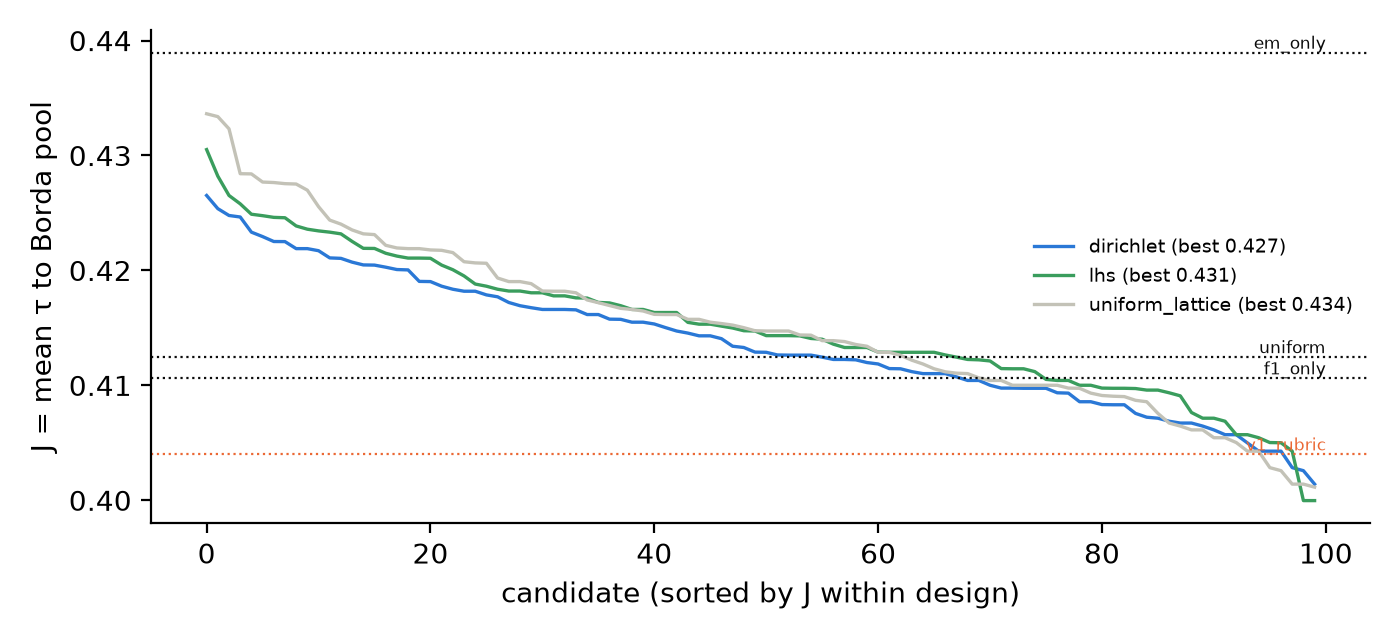
\includegraphics[width=0.85\textwidth]{fig_landscape.png}\caption{All 305 candidates sorted by $J$, with the baselines marked.}\label{fig:fig_landscape}\end{figure}
\begin{figure}[htbp]\centering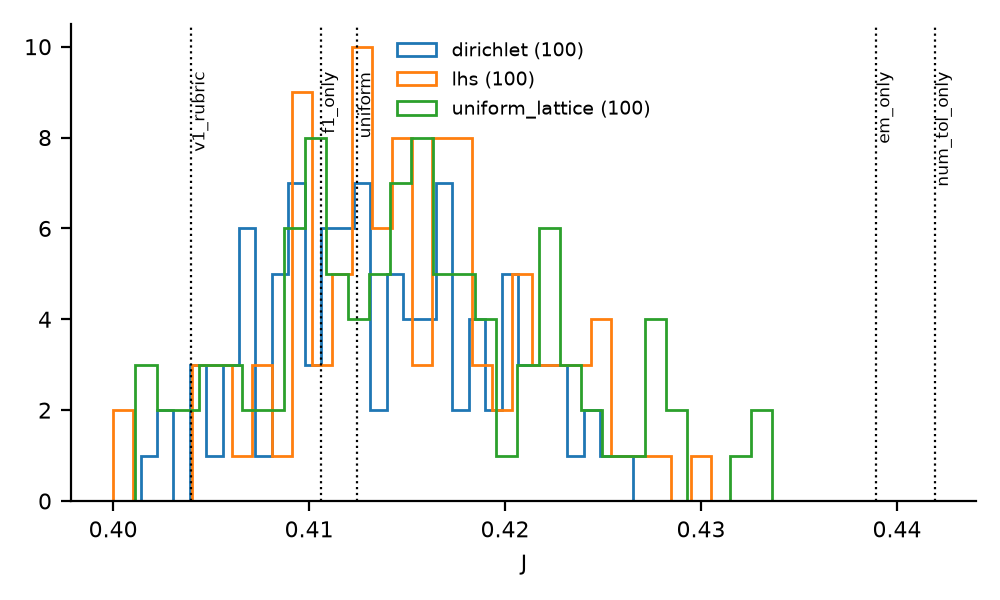
\includegraphics[width=0.6\textwidth]{fig_j_by_design.png}\caption{Distribution of $J$ over the 100 candidates of each design, with the five baselines marked.}\label{fig:fig_j_by_design}\end{figure}
\begin{figure}[htbp]\centering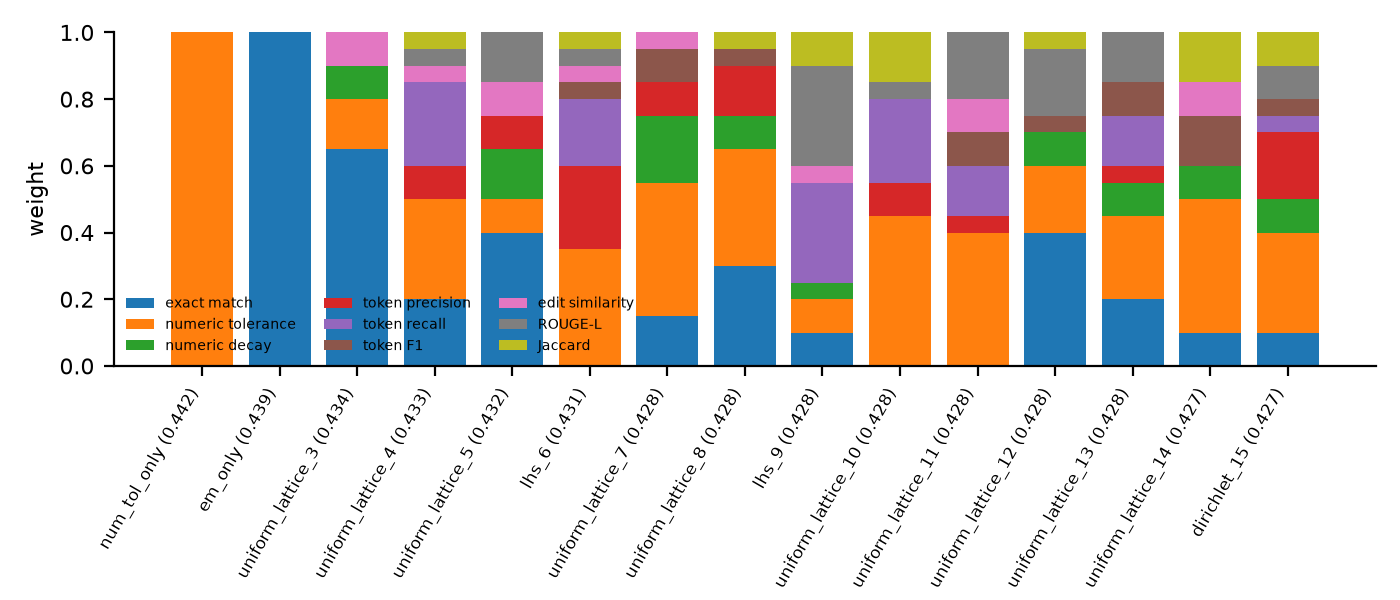
\includegraphics[width=0.85\textwidth]{fig_top_weights.png}\caption{Component weights of the fifteen best candidates.}\label{fig:fig_top_weights}\end{figure}
\begin{landscape}
\begin{table}[htbp]
\centering\tiny
\caption{Sampled designs: summary over 20 seeds.}
\label{tab:designs_summary}
\setlength{\tabcolsep}{3pt}
\resizebox{\linewidth}{!}{%
\begin{tabular}{lrrrrrrrrrr}
\toprule
design & best\_\allowbreak{}J\_\allowbreak{}mean & best\_\allowbreak{}J\_\allowbreak{}sd & best\_\allowbreak{}J\_\allowbreak{}max & mean\_\allowbreak{}J & regret\_\allowbreak{}mean & regret\_\allowbreak{}max & min\_\allowbreak{}pairwise\_\allowbreak{}L1 & mean\_\allowbreak{}nearest\_\allowbreak{}L1 & discrepancy & zero\_\allowbreak{}share \\
\midrule
dirichlet\_\allowbreak{}lattice & 0.4320 & 0.0030 & 0.4391 & 0.4153 & 0.0100 & 0.0138 & 0.1950 & 0.4027 & 2.6738 & 0.8820 \\
lhs\_\allowbreak{}simplex & 0.4313 & 0.0022 & 0.4373 & 0.4151 & 0.0107 & 0.0141 & 0.2150 & 0.4096 & 2.6718 & 0.8780 \\
uniform\_\allowbreak{}lattice & 0.4343 & 0.0033 & 0.4420 & 0.4155 & 0.0077 & 0.0129 & 0.2350 & 0.4650 & 2.5904 & 0.9705 \\
\bottomrule
\end{tabular}
}
\end{table}
\end{landscape}

\begin{figure}[htbp]\centering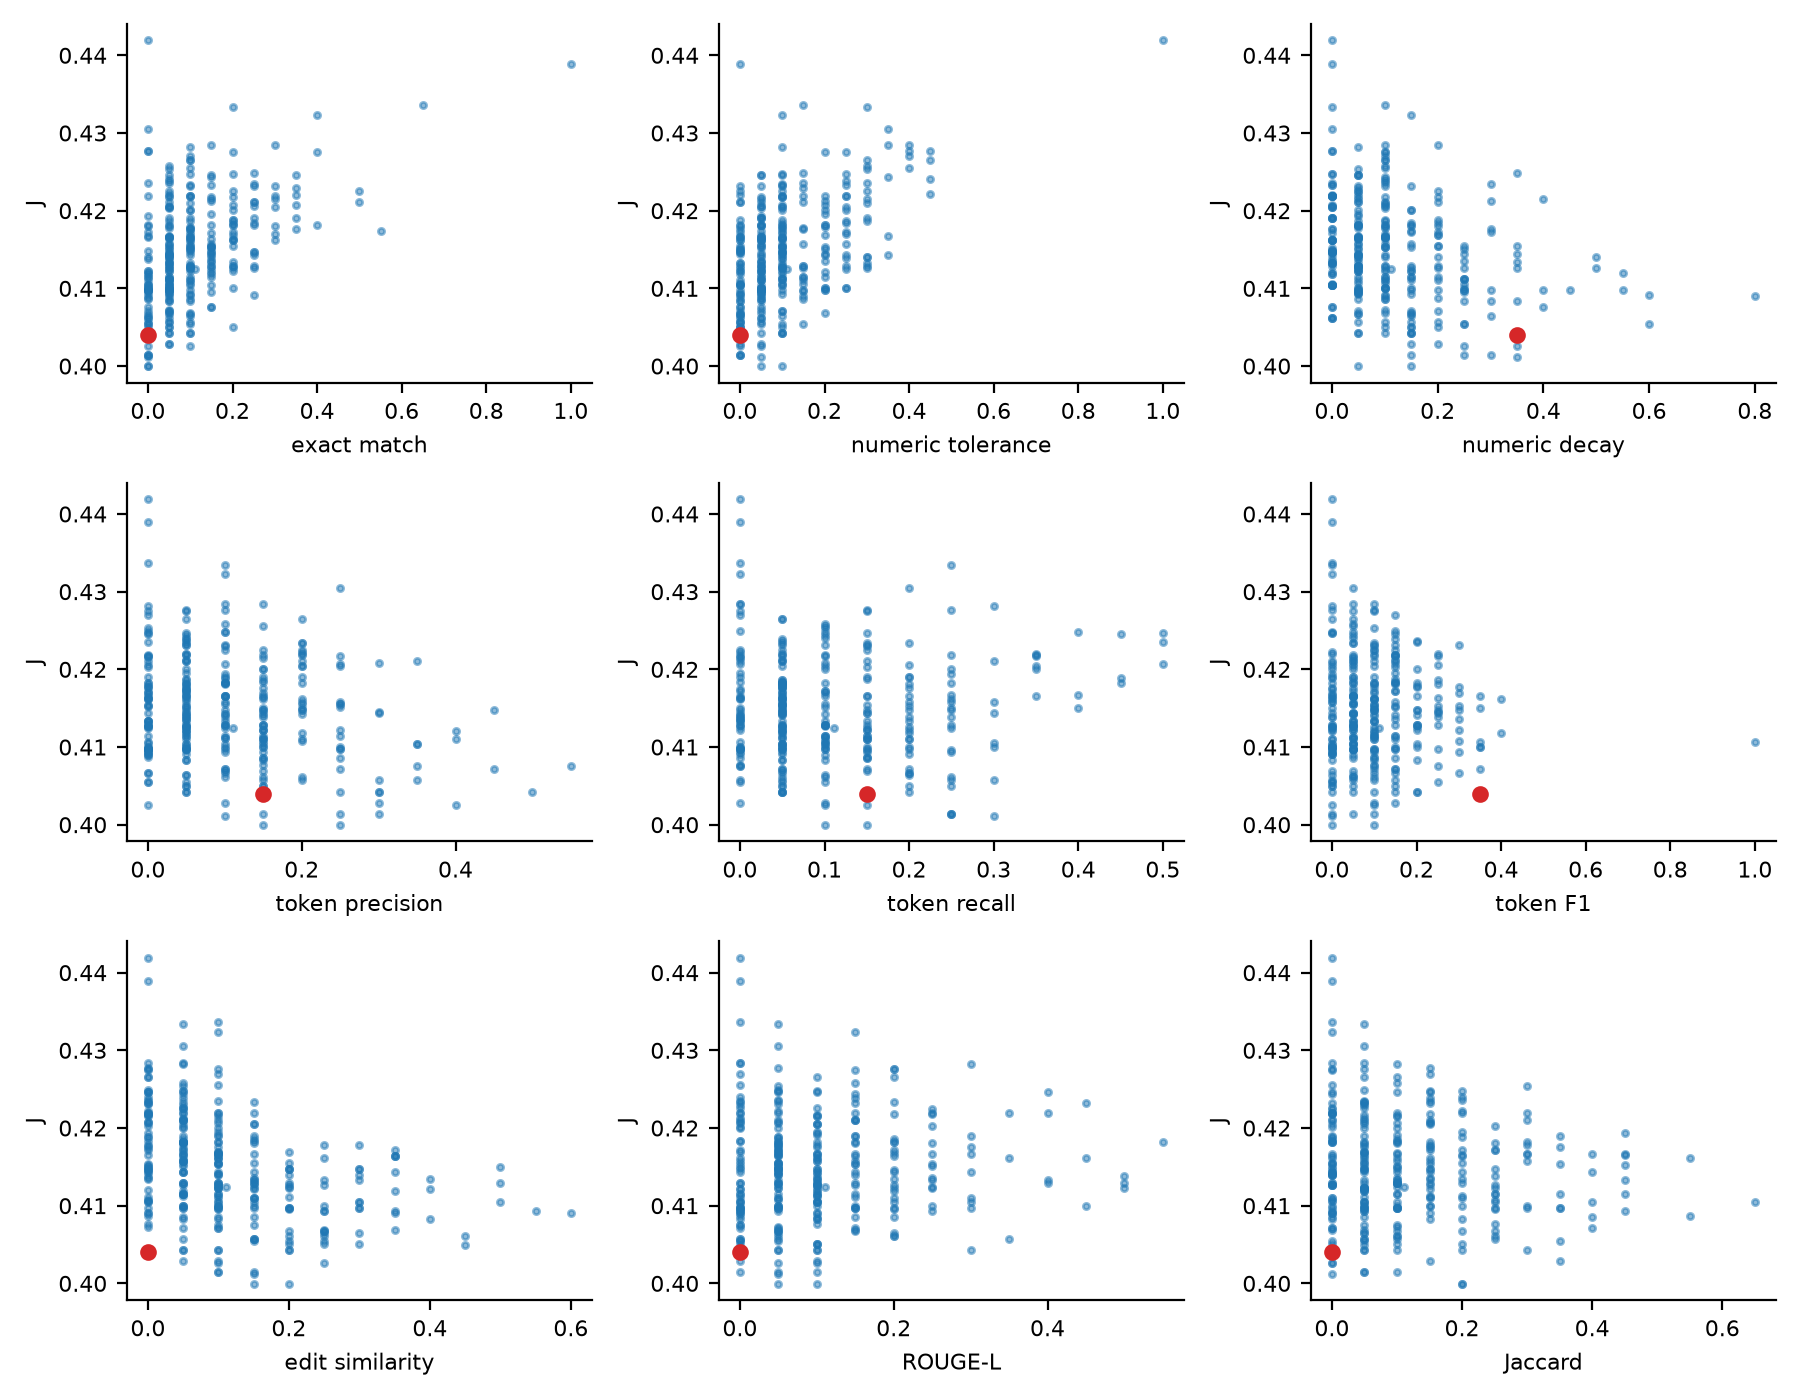
\includegraphics[width=0.85\textwidth]{fig_marginals.png}\caption{$J$ against each component weight over all candidates; red = v1 rubric.}\label{fig:fig_marginals}\end{figure}


\subsection{Honest selection}
As in v2, the in-bag winner loses 0.050 out of bag and ends -0.002 from the v1 rubric with an interval that includes zero; 204 different candidates are selected across resamples and the plateau covers 305 of 305 (Figures~\ref{fig:fig_nested}, \ref{fig:fig_oob_difference}, \ref{fig:fig_selected_weights}).
\begin{figure}[htbp]\centering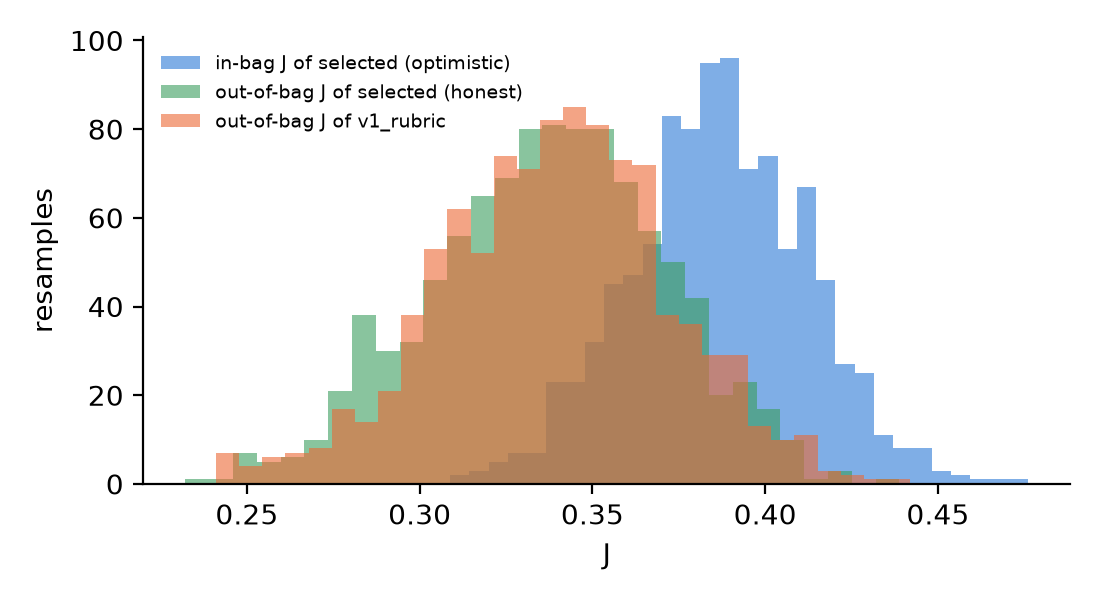
\includegraphics[width=0.6\textwidth]{fig_nested.png}\caption{In-bag vs out-of-bag $J$ of the selected candidate against the v1 rubric.}\label{fig:fig_nested}\end{figure}
\begin{figure}[htbp]\centering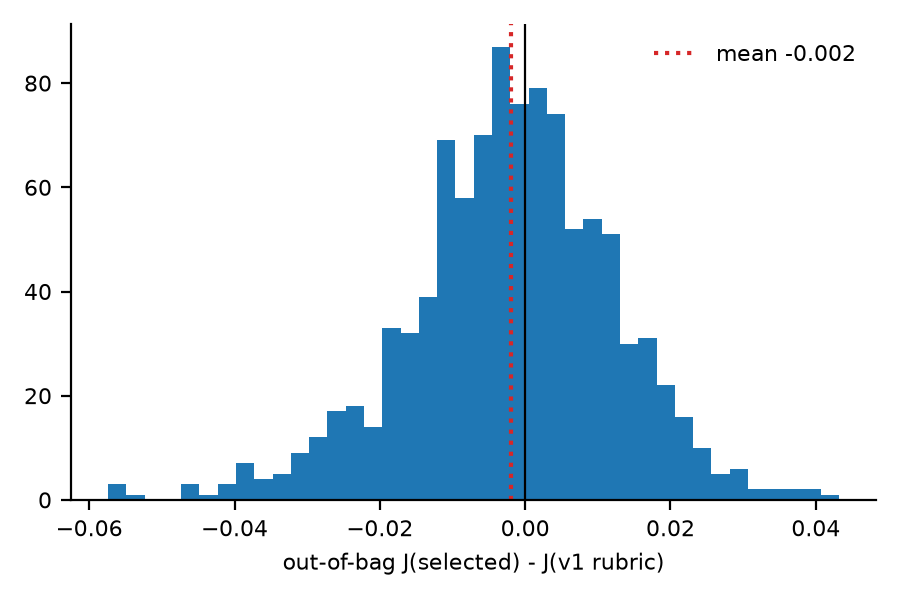
\includegraphics[width=0.5\textwidth]{fig_oob_difference.png}\caption{Paired out-of-bag difference between the selected candidate and the v1 rubric over 1,000 resamples.}\label{fig:fig_oob_difference}\end{figure}
\begin{figure}[htbp]\centering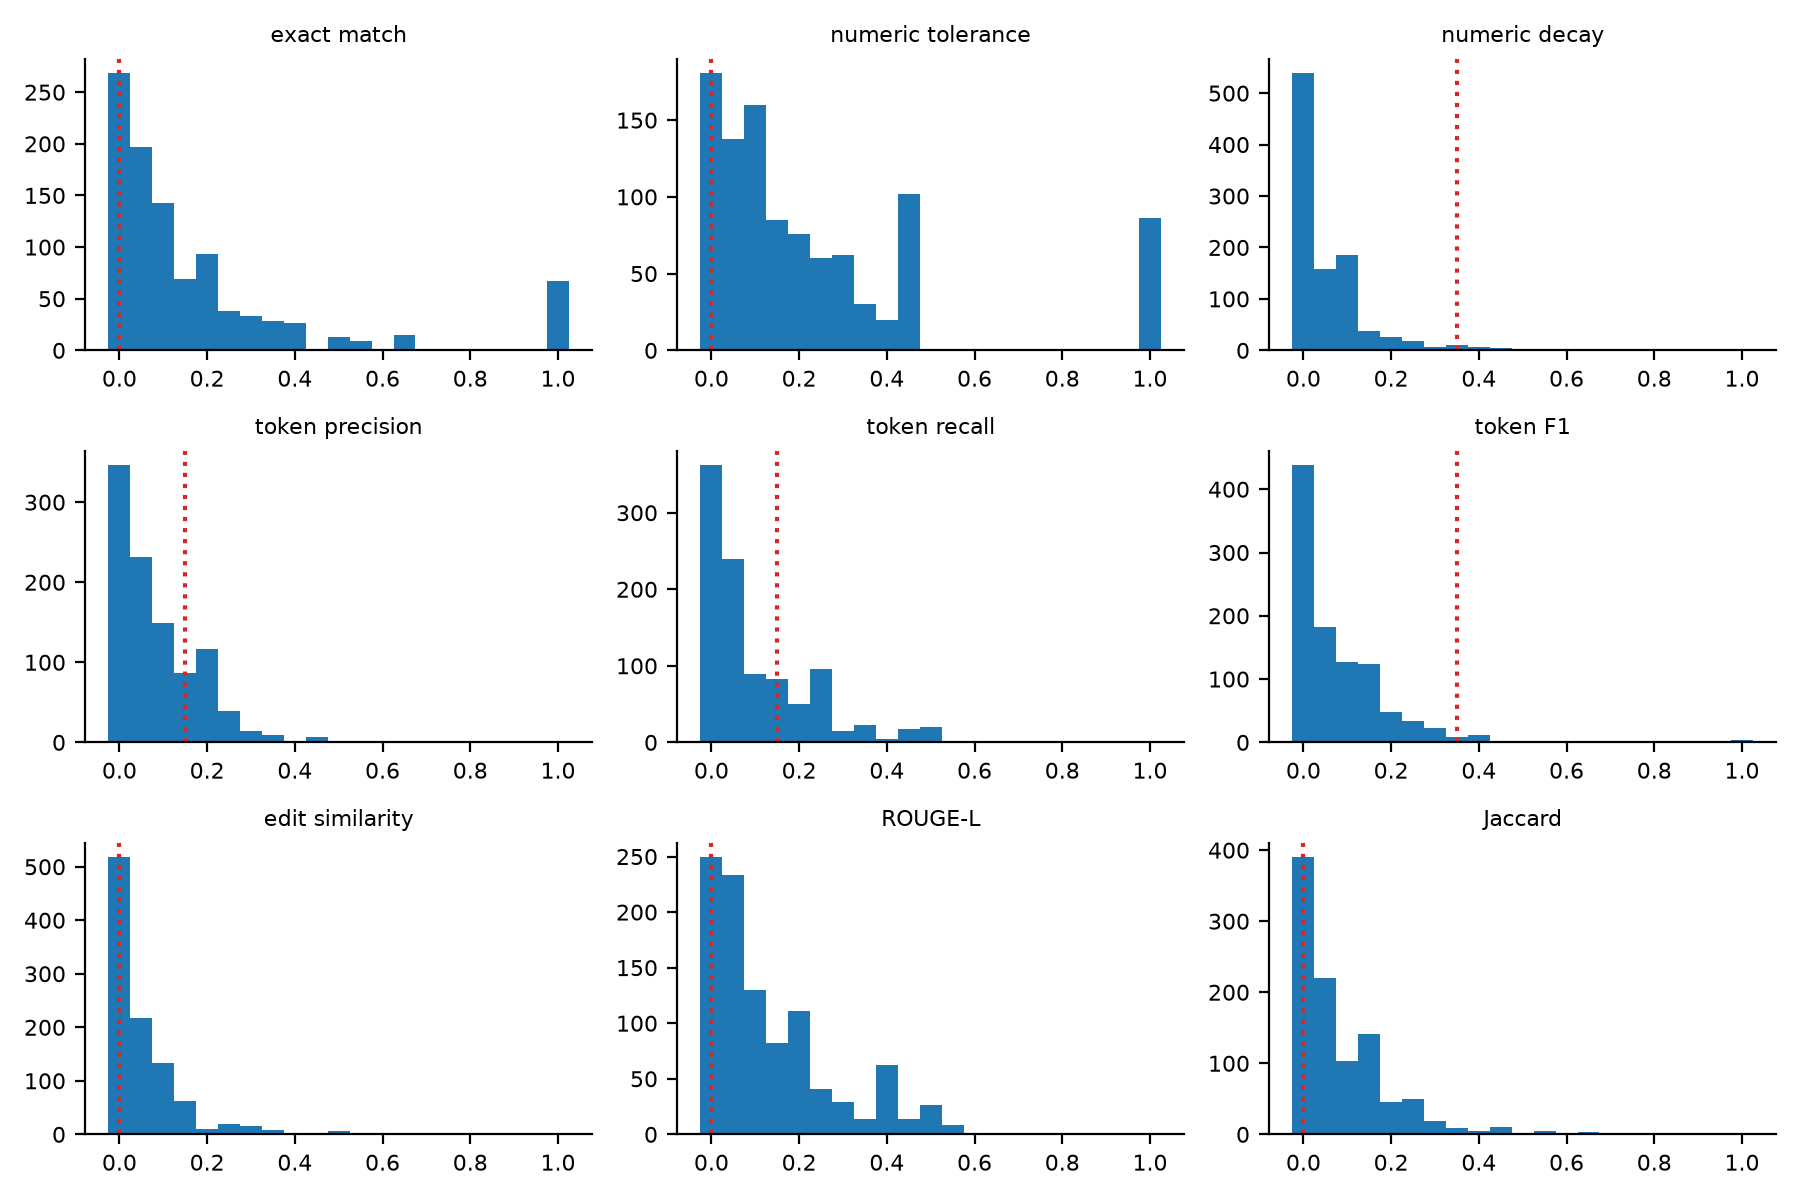
\includegraphics[width=0.85\textwidth]{fig_selected_weights.png}\caption{Weights selected as in-bag best across 1,000 bootstrap resamples; dotted = v1 rubric.}\label{fig:fig_selected_weights}\end{figure}


\subsection{Transfer}
Re-fitted weights predict a held-out dataset no better than the v1 rubric (Figure~\ref{fig:fig_lodo_tau}); the per-family optima are numeric tolerance for EM and SM but recall- and precision-heavy mixes for TQA and FIN (Figure~\ref{fig:fig_family_weights}, Table~\ref{tab:per_family}).
\begin{figure}[htbp]\centering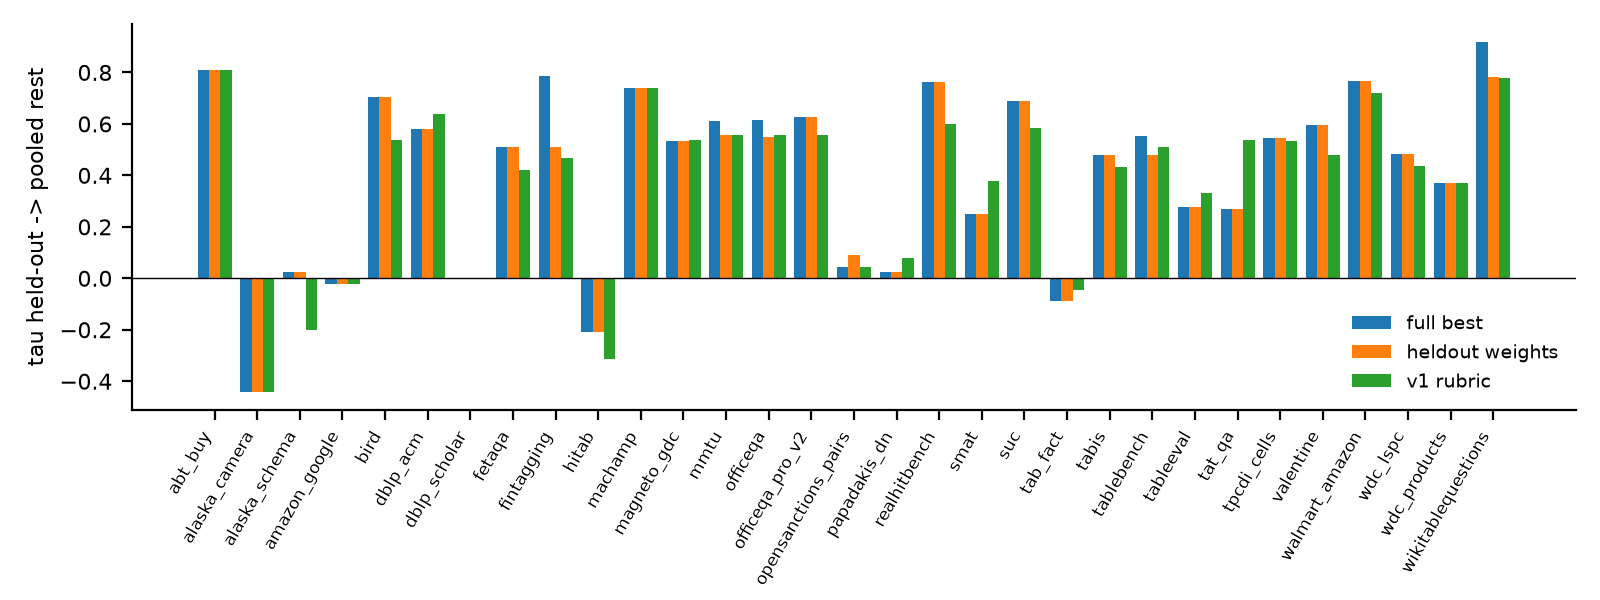
\includegraphics[width=0.85\textwidth]{fig_lodo_tau.png}\caption{Leave-one-dataset-out: agreement of the held-out dataset with the pooled rest under re-fitted weights, the full best and the v1 rubric.}\label{fig:fig_lodo_tau}\end{figure}
\begin{figure}[htbp]\centering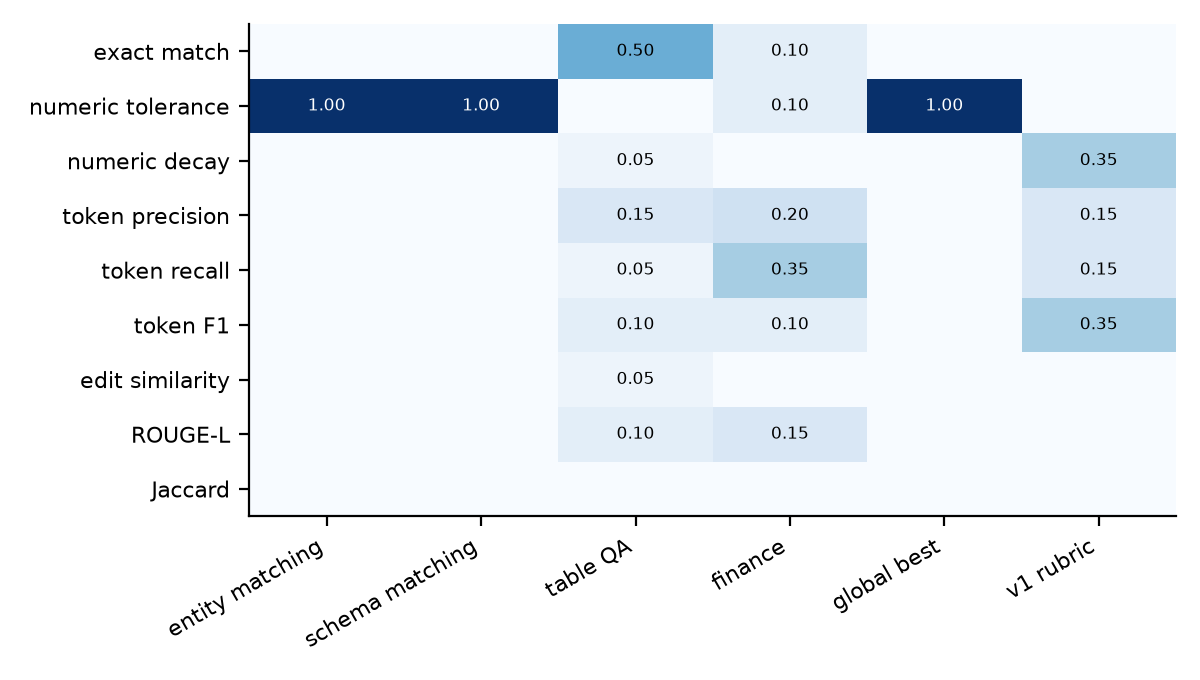
\includegraphics[width=0.7\textwidth]{fig_family_weights.png}\caption{Per-family optimum, global optimum and the v1 rubric over the nine components.}\label{fig:fig_family_weights}\end{figure}
\begin{table}[htbp]
\centering\scriptsize
\caption{Per-family optimum.}
\label{tab:per_family}
\setlength{\tabcolsep}{3pt}
\begin{tabular}{lp{0.739\linewidth}rp{0.075\linewidth}}
\toprule
family & best weights & J own best & J global best \\
\midrule
EM & numeric tolerance 1.00 & 0.361 & 0.361 \\
SM & numeric tolerance 1.00 & 0.580 & 0.580 \\
TQA & exact match 0.50, numeric decay 0.05, token precision 0.15, token recall 0.05, token F1 0.10, edit similarity 0.05, ROUGE-L 0.10 & 0.513 & 0.512 \\
FIN & exact match 0.10, numeric tolerance 0.10, token precision 0.20, token recall 0.35, token F1 0.10, ROUGE-L 0.15 & 0.834 & 0.619 \\
\bottomrule
\end{tabular}
\end{table}



\subsection{Correctness}
Numeric tolerance alone is the best by $J$ but the worst labelled rule on the anchors ($\rho$ = 0.796 vs 0.878 for the v1 rubric): it gives no partial credit to near misses, which the anchors reward (Figure~\ref{fig:fig_anchor_operators}). The Pareto knee (em 0.40, num\_\allowbreak{}tol 0.10, num\_\allowbreak{}decay 0.15, tok\_\allowbreak{}prec 0.10, edit\_\allowbreak{}sim 0.10, rouge\_\allowbreak{}l 0.15) keeps $J$ = 0.432 and $\rho$ = 0.884. Across candidates $J$ and $\rho$ correlate -0.19: agreement and correctness pull apart here as in v2.
\begin{landscape}
\begin{table}[htbp]
\centering\tiny
\caption{Anchor correctness for the labelled candidates.}
\label{tab:anchors_rules}
\setlength{\tabcolsep}{3pt}
\resizebox{\linewidth}{!}{%
\begin{tabular}{lrrrrrrrrrrrrrrr}
\toprule
label & w\_\allowbreak{}em & w\_\allowbreak{}num\_\allowbreak{}tol & w\_\allowbreak{}num\_\allowbreak{}decay & w\_\allowbreak{}tok\_\allowbreak{}prec & w\_\allowbreak{}tok\_\allowbreak{}rec & w\_\allowbreak{}tok\_\allowbreak{}f1 & w\_\allowbreak{}edit\_\allowbreak{}sim & w\_\allowbreak{}rouge\_\allowbreak{}l & w\_\allowbreak{}jaccard & J & rho & rho\_\allowbreak{}ds & auc & wrong\_\allowbreak{}mean & hedge\_\allowbreak{}gap \\
\midrule
num\_\allowbreak{}tol\_\allowbreak{}only & 0.000 & 1.000 & 0.000 & 0.000 & 0.000 & 0.000 & 0.000 & 0.000 & 0.000 & 0.442 & 0.796 & 0.808 & 0.989 & 0.022 & -0.595 \\
em\_\allowbreak{}only & 1.000 & 0.000 & 0.000 & 0.000 & 0.000 & 0.000 & 0.000 & 0.000 & 0.000 & 0.439 & 0.828 & 0.830 & 0.989 & 0.011 & -0.807 \\
uniform & 0.111 & 0.111 & 0.111 & 0.111 & 0.111 & 0.111 & 0.111 & 0.111 & 0.111 & 0.412 & 0.878 & 0.861 & 0.994 & 0.046 & -0.555 \\
f1\_\allowbreak{}only & 0.000 & 0.000 & 0.000 & 0.000 & 0.000 & 1.000 & 0.000 & 0.000 & 0.000 & 0.411 & 0.856 & 0.846 & 0.989 & 0.030 & -0.496 \\
v1\_\allowbreak{}rubric & 0.000 & 0.000 & 0.350 & 0.150 & 0.150 & 0.350 & 0.000 & 0.000 & 0.000 & 0.404 & 0.878 & 0.868 & 0.994 & 0.034 & -0.506 \\
\bottomrule
\end{tabular}
}
\end{table}
\end{landscape}

\begin{figure}[htbp]\centering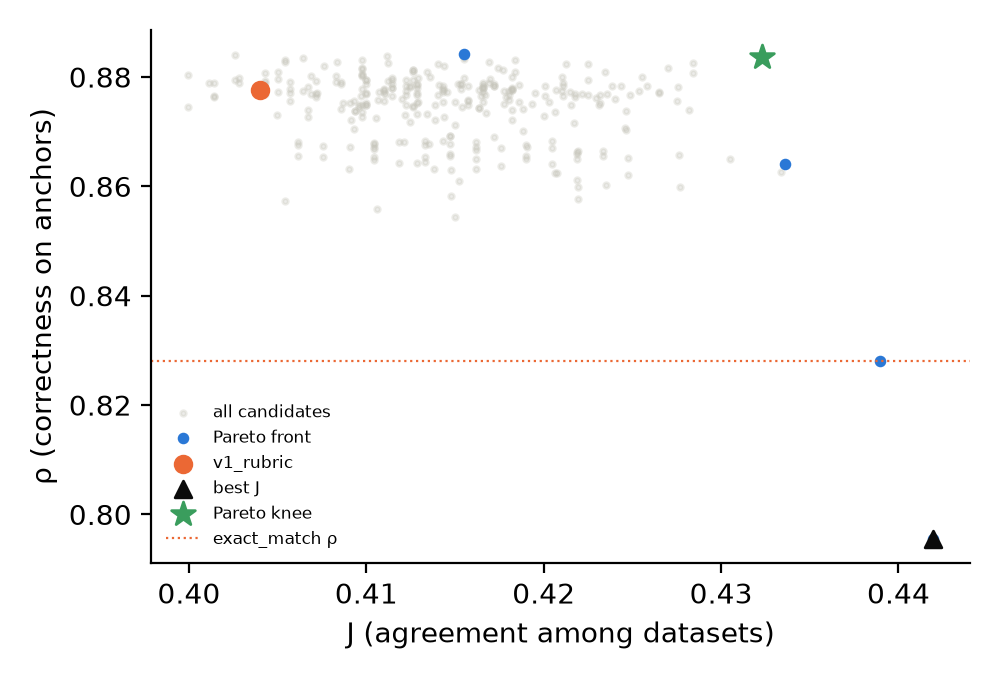
\includegraphics[width=0.7\textwidth]{fig_pareto.png}\caption{Agreement $J$ against anchor correctness $\rho$ for every candidate.}\label{fig:fig_pareto}\end{figure}
\begin{figure}[htbp]\centering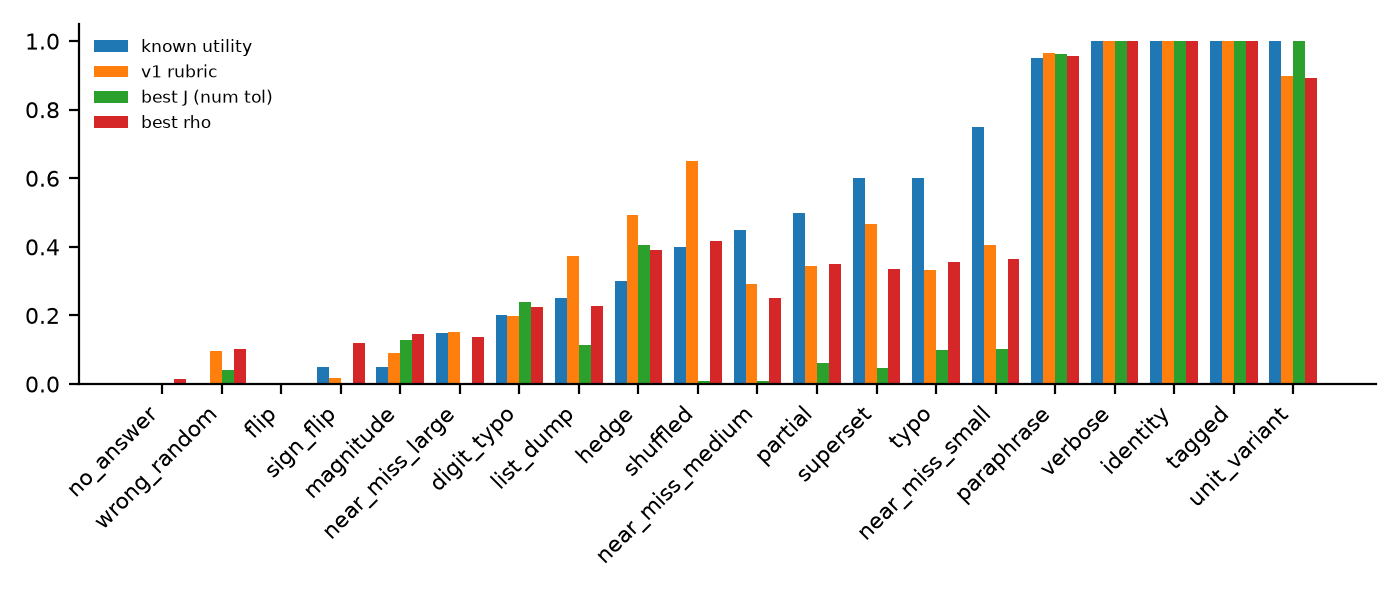
\includegraphics[width=0.85\textwidth]{fig_anchor_operators.png}\caption{Anchors: known utility of each operator against the mean score it receives under the v1 rubric, the best-$J$ and the best-$\rho$ candidates.}\label{fig:fig_anchor_operators}\end{figure}


\subsection{Leaderboard}
Under the v1 rubric the ranking is the one v2 reports (same answers, same rule): Gemini 3.8 Flash first by Bradley--Terry, GPT-5.5 first by Borda, Llama 3.3 70B last. Under the best-$J$ rule (numeric tolerance) and under exact match Claude Opus 5 is first. Rule choice moves the top three and nothing else.
\begin{table}[htbp]
\centering\tiny
\caption{Leaderboard under the headline rule (v1 rubric).}
\label{tab:leaderboard_headline}
\setlength{\tabcolsep}{3pt}
\begin{tabular}{lp{0.256\linewidth}p{0.176\linewidth}rrrp{0.176\linewidth}r}
\toprule
rank & model & BT strength & SE & Borda rank & Borda 95\% & P(first) BT & mean score \\
\midrule
1 & Gemini 3.8 Flash & 0.121 & 0.016 & 3 & [1, 3] & 0.990 & 0.812 \\
2 & Claude Opus 5 & 0.095 & 0.000 & 2 & [1, 3] & 0.010 & 0.811 \\
3 & GPT-5.5 & 0.052 & 0.016 & 1 & [1, 3] & 0.000 & 0.808 \\
4 & Claude Sonnet 5 & 0.029 & 0.016 & 4 & [4, 6] & 0.000 & 0.795 \\
5 & Grok 4 & 0.027 & 0.016 & 5 & [4, 6] & 0.000 & 0.797 \\
6 & GPT-5.4-mini & -0.010 & 0.016 & 8 & [5, 8] & 0.000 & 0.790 \\
7 & DeepSeek-chat & -0.018 & 0.016 & 7 & [5, 8] & 0.000 & 0.784 \\
8 & DeepSeek-R1 & -0.025 & 0.016 & 6 & [5, 8] & 0.000 & 0.788 \\
9 & gpt-oss-120b & -0.100 & 0.016 & 9 & [9, 10] & 0.000 & 0.767 \\
10 & Llama 3.3 70B & -0.170 & 0.016 & 10 & [9, 10] & 0.000 & 0.738 \\
\bottomrule
\end{tabular}
\end{table}

\begin{landscape}
\begin{table}[htbp]
\centering\tiny
\caption{Bradley--Terry rank (Borda rank in brackets) under each reported rule, Friedman $p$ and Kendall's $W$ among datasets.}
\label{tab:ranks_by_rule}
\setlength{\tabcolsep}{3pt}
\resizebox{\linewidth}{!}{%
\begin{tabular}{lrrrrrrrrrrrr}
\toprule
rule & Gemini 3.8 Flash & Claude Opus 5 & GPT-5.5 & Claude Sonnet 5 & Grok 4 & GPT-5.4-mini & DeepSeek-chat & DeepSeek-R1 & gpt-oss-120b & Llama 3.3 70B & Friedman p & W \\
\midrule
exact match & 3 (3) & 1 (1) & 2 (2) & 5 (4) & 4 (5) & 6 (8) & 8 (7) & 7 (6) & 9 (9) & 10 (10) & 5.3e-14 & 0.28 \\
v1 rubric & 1 (3) & 2 (2) & 3 (1) & 4 (4) & 5 (5) & 6 (8) & 7 (7) & 8 (6) & 9 (9) & 10 (10) & 1.0e-12 & 0.26 \\
top1 & 3 (3) & 1 (1) & 2 (2) & 5 (4) & 4 (5) & 6 (7) & 8 (8) & 7 (6) & 9 (9) & 10 (10) & 7.2e-14 & 0.28 \\
top2 & 3 (3) & 1 (1) & 2 (2) & 5 (4) & 4 (5) & 6 (8) & 8 (7) & 7 (6) & 9 (9) & 10 (10) & 5.3e-14 & 0.28 \\
top3 & 1 (3) & 2 (1) & 3 (2) & 4 (4) & 5 (5) & 6 (7) & 7 (8) & 8 (6) & 9 (9) & 10 (10) & 9.2e-14 & 0.28 \\
top4 & 1 (3) & 2 (1) & 3 (2) & 5 (4) & 4 (5) & 7 (8) & 6 (7) & 8 (6) & 9 (9) & 10 (10) & 8.5e-14 & 0.28 \\
top5 & 1 (3) & 2 (1) & 3 (1) & 4 (4) & 5 (5) & 6 (7) & 7 (8) & 8 (6) & 9 (9) & 10 (10) & 1.1e-13 & 0.28 \\
best-rho & 1 (3) & 2 (2) & 3 (1) & 4 (4) & 5 (5) & 6 (7) & 7 (8) & 8 (6) & 9 (9) & 10 (10) & 3.6e-13 & 0.27 \\
knee & 1 (3) & 2 (1) & 3 (1) & 4 (4) & 5 (5) & 6 (7) & 7 (8) & 8 (6) & 9 (9) & 10 (10) & 1.1e-13 & 0.28 \\
\bottomrule
\end{tabular}
}
\end{table}
\end{landscape}

\begin{figure}[htbp]\centering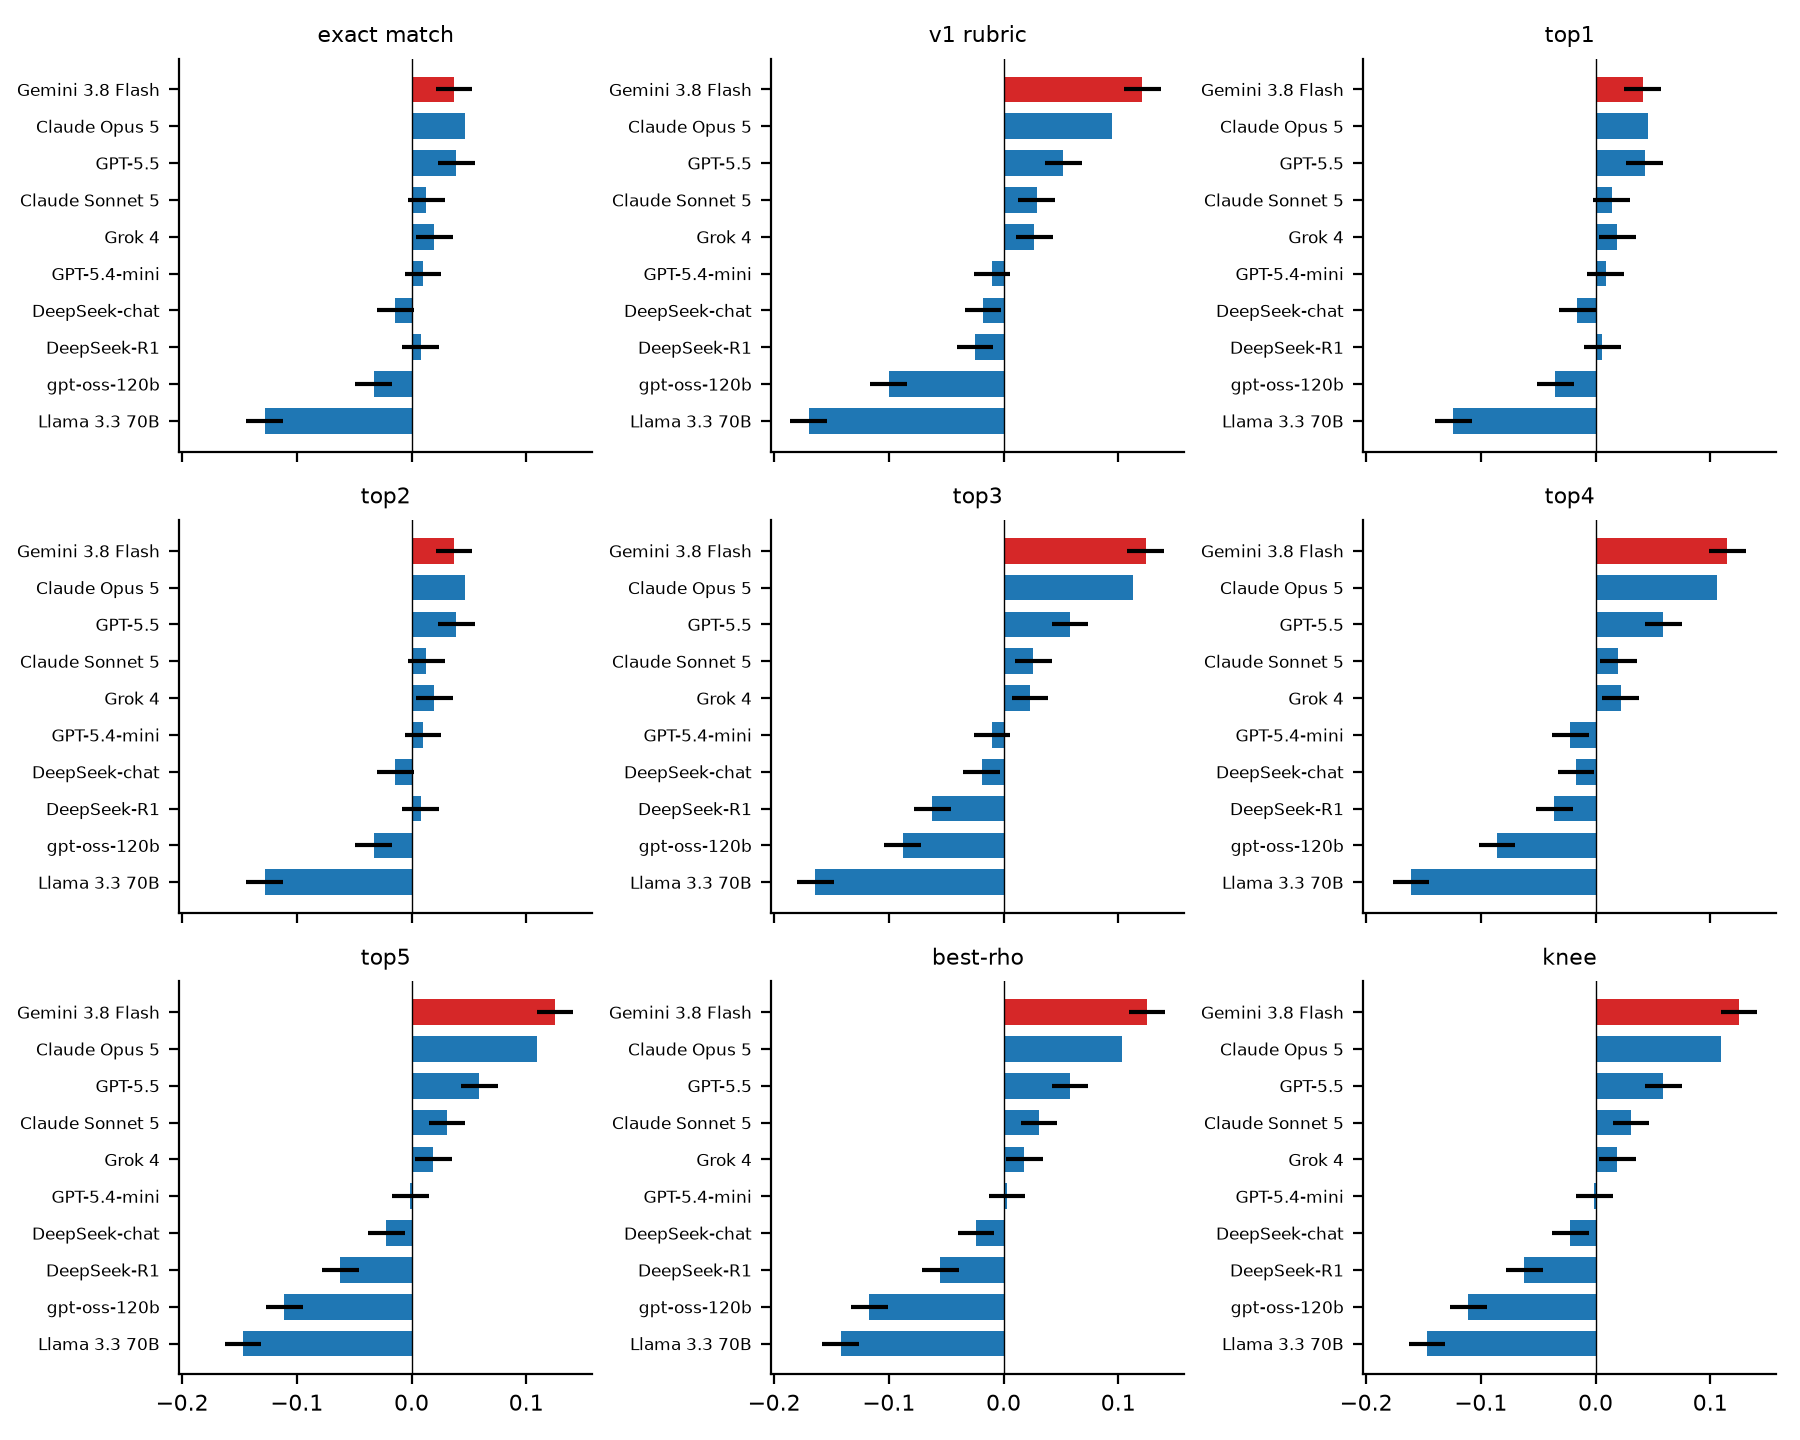
\includegraphics[width=0.85\textwidth]{fig_bt_all_rules.png}\caption{Bradley--Terry strengths ($\pm$ SE vs reference) under every reported rule; models fixed in the headline order.}\label{fig:fig_bt_all_rules}\end{figure}
\begin{figure}[htbp]\centering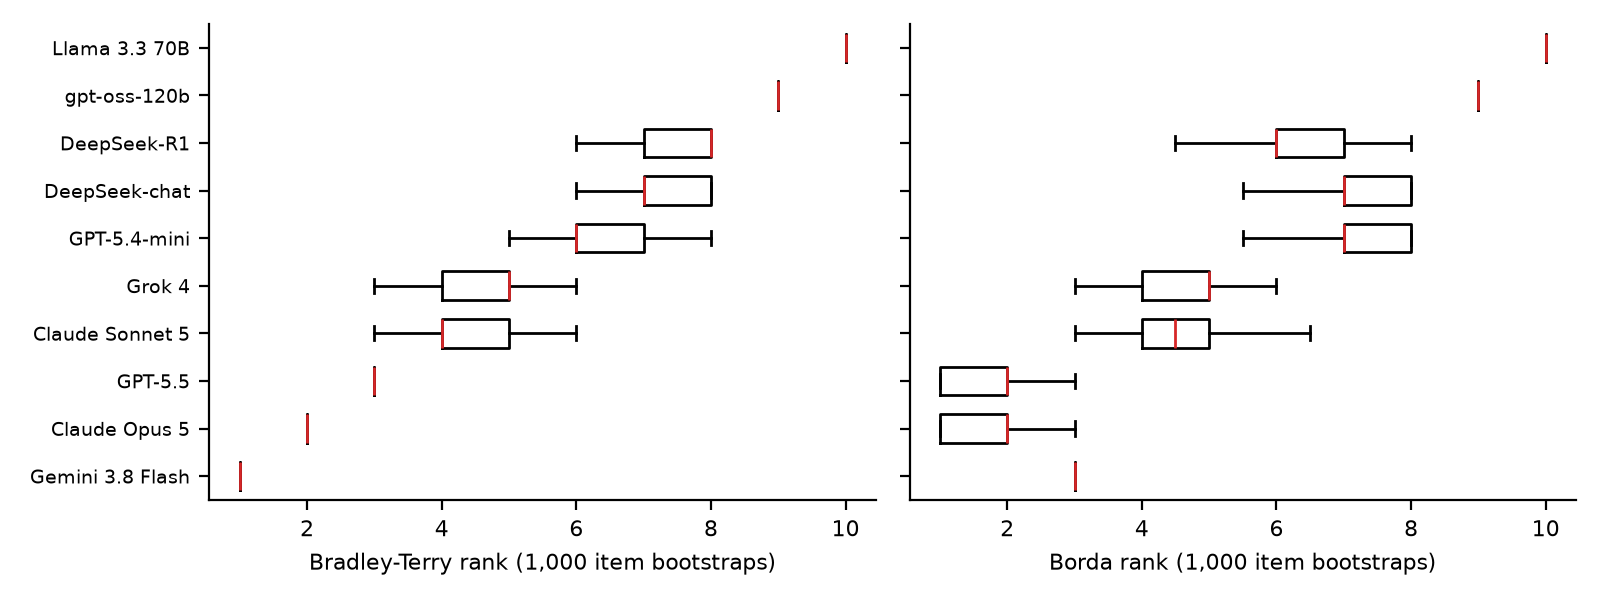
\includegraphics[width=0.85\textwidth]{fig_rank_bootstrap.png}\caption{Bootstrap distribution of each model's rank under the headline rule (v1 rubric).}\label{fig:fig_rank_bootstrap}\end{figure}


\subsection{Comparability and diagnostics}
\begin{table}[htbp]
\centering\tiny
\caption{Official-split estimates under the headline rule averaged over the ten models.}
\label{tab:official_split_by_dataset}
\setlength{\tabcolsep}{3pt}
\begin{tabular}{p{0.121\linewidth}rp{0.108\linewidth}p{0.076\linewidth}p{0.140\linewidth}p{0.121\linewidth}p{0.095\linewidth}p{0.146\linewidth}}
\toprule
dataset & suite\_\allowbreak{}mean & official\_\allowbreak{}estimate & suite\_\allowbreak{}f1\_\allowbreak{}pos & official\_\allowbreak{}precision\_\allowbreak{}pos & official\_\allowbreak{}recall\_\allowbreak{}pos & official\_\allowbreak{}f1\_\allowbreak{}pos & official\_\allowbreak{}positive\_\allowbreak{}share \\
\midrule
abt\_\allowbreak{}buy & 0.970 & 0.986 & 0.968 & 0.926 & 0.949 & 0.936 & 0.108 \\
alaska\_\allowbreak{}camera & 0.958 & 0.958 & 0.955 & 1.000 & 0.921 & 0.955 & 0.500 \\
alaska\_\allowbreak{}schema & 0.928 & 0.928 & -- & -- & -- & -- & -- \\
amazon\_\allowbreak{}google & 0.936 & 0.932 & 0.929 & 0.611 & 0.942 & 0.739 & 0.102 \\
bird & 0.187 & 0.213 & -- & -- & -- & -- & -- \\
dblp\_\allowbreak{}acm & 0.986 & 0.991 & 0.985 & 0.979 & 0.978 & 0.976 & 0.180 \\
dblp\_\allowbreak{}scholar & 0.949 & 0.966 & 0.948 & 0.900 & 0.924 & 0.910 & 0.186 \\
fetaqa & 0.382 & 0.382 & -- & -- & -- & -- & -- \\
fintagging & 0.880 & 0.876 & -- & -- & -- & -- & -- \\
hitab & 0.770 & 0.773 & -- & -- & -- & -- & -- \\
machamp & 0.887 & 0.890 & 0.892 & 0.644 & 0.853 & 0.733 & 0.175 \\
magneto\_\allowbreak{}gdc & 0.934 & 0.938 & -- & -- & -- & -- & -- \\
mmtu & 0.867 & 0.829 & -- & -- & -- & -- & -- \\
officeqa & 0.129 & 0.129 & -- & -- & -- & -- & -- \\
officeqa\_\allowbreak{}pro\_\allowbreak{}v2 & 0.139 & 0.139 & -- & -- & -- & -- & -- \\
opensanctions\_\allowbreak{}pairs & 0.821 & 0.727 & 0.773 & 0.993 & 0.649 & 0.777 & 0.769 \\
papadakis\_\allowbreak{}dn & 0.941 & 0.988 & 0.833 & 0.550 & 0.963 & 0.683 & 0.018 \\
realhitbench & 0.673 & 0.673 & -- & -- & -- & -- & -- \\
smat & 0.918 & 0.916 & -- & -- & -- & -- & -- \\
suc & 0.914 & 0.912 & -- & -- & -- & -- & -- \\
tab\_\allowbreak{}fact & 0.798 & 0.789 & 0.758 & 0.896 & 0.674 & 0.764 & 0.500 \\
tabis & 0.915 & 0.918 & -- & -- & -- & -- & -- \\
tablebench & 0.818 & 0.816 & -- & -- & -- & -- & -- \\
tableeval & 0.749 & 0.754 & -- & -- & -- & -- & -- \\
tat\_\allowbreak{}qa & 0.803 & 0.758 & -- & -- & -- & -- & -- \\
tpcdi\_\allowbreak{}cells & 0.456 & 0.461 & -- & -- & -- & -- & -- \\
valentine & 0.984 & 0.979 & -- & -- & -- & -- & -- \\
walmart\_\allowbreak{}amazon & 0.958 & 0.975 & 0.947 & 0.832 & 0.927 & 0.875 & 0.094 \\
wdc\_\allowbreak{}lspc & 0.982 & 0.983 & 0.983 & 0.965 & 0.979 & 0.971 & 0.264 \\
wdc\_\allowbreak{}products & 0.978 & 0.985 & 0.979 & 0.980 & 0.968 & 0.974 & 0.280 \\
wikitablequestions & 0.846 & 0.844 & -- & -- & -- & -- & -- \\
\bottomrule
\end{tabular}
\end{table}

\begin{figure}[htbp]\centering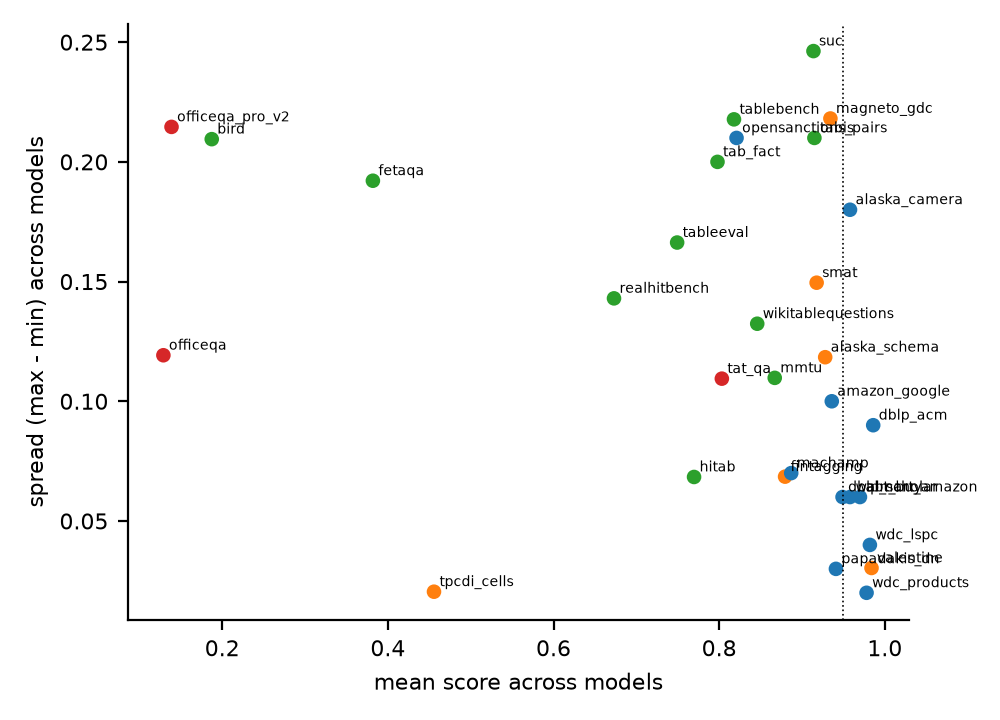
\includegraphics[width=0.6\textwidth]{fig_diagnostics_scatter.png}\caption{Dataset diagnostics: mean score against spread across models; dotted line marks the ceiling flag.}\label{fig:fig_diagnostics_scatter}\end{figure}


\clearpage
\appendix
\section{All figures}
Every figure that can be drawn from the saved outputs; source data in \texttt{data/}.
\begin{figure}[htbp]\centering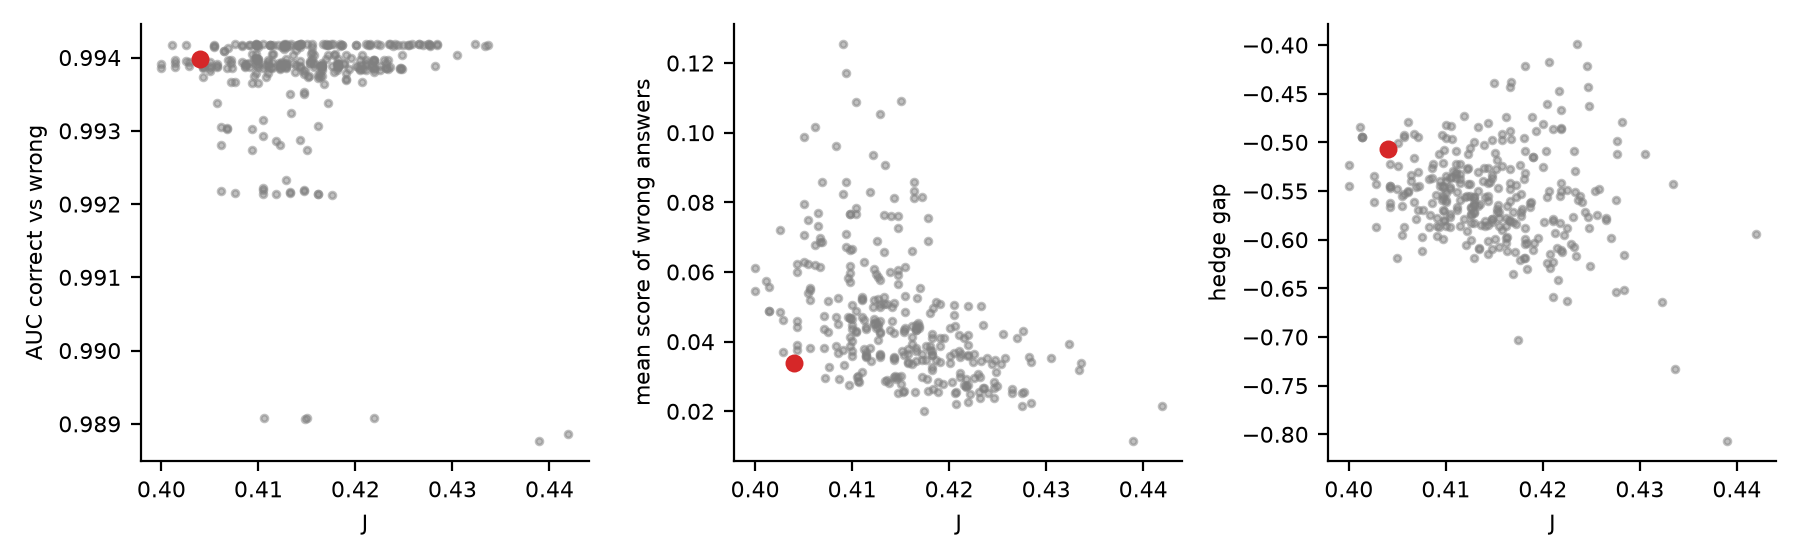
\includegraphics[width=0.9\textwidth]{fig_anchor_metrics_vs_j.png}\caption{Three further anchor diagnostics against $J$ for every candidate (red = v1 rubric).}\label{figall:fig_anchor_metrics_vs_j}\end{figure}
\begin{figure}[htbp]\centering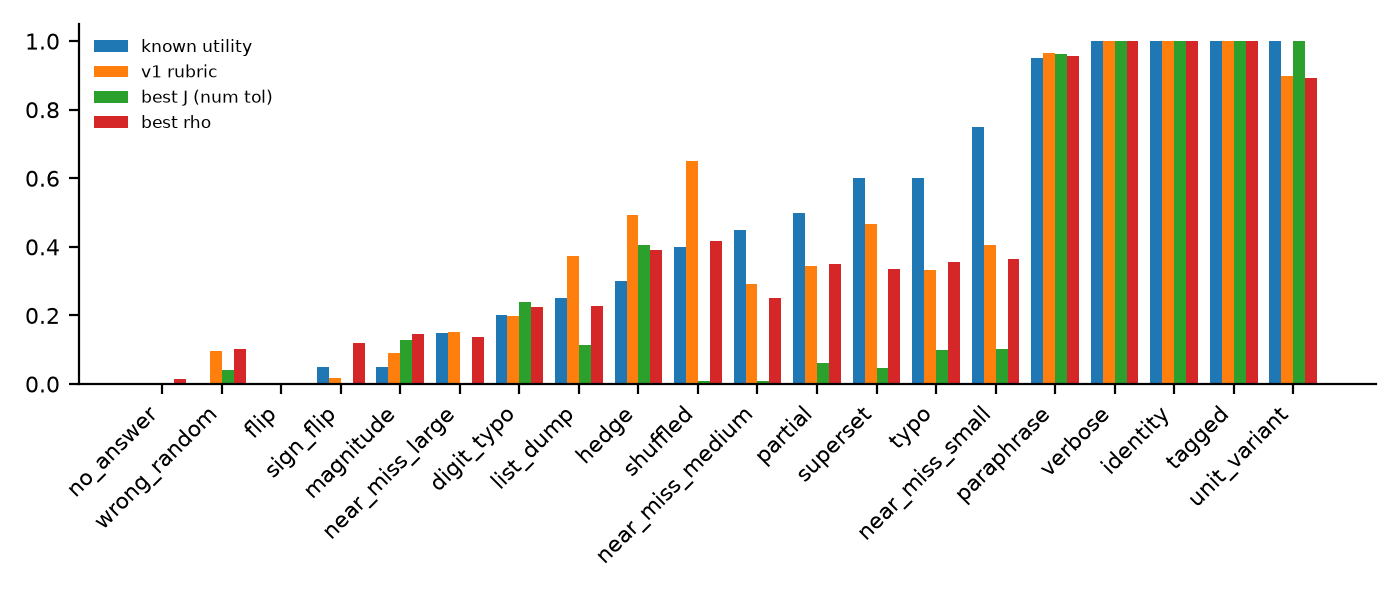
\includegraphics[width=0.9\textwidth]{fig_anchor_operators.png}\caption{Anchors: known utility of each operator against the mean score it receives under the v1 rubric, the best-$J$ and the best-$\rho$ candidates.}\label{figall:fig_anchor_operators}\end{figure}
\begin{figure}[htbp]\centering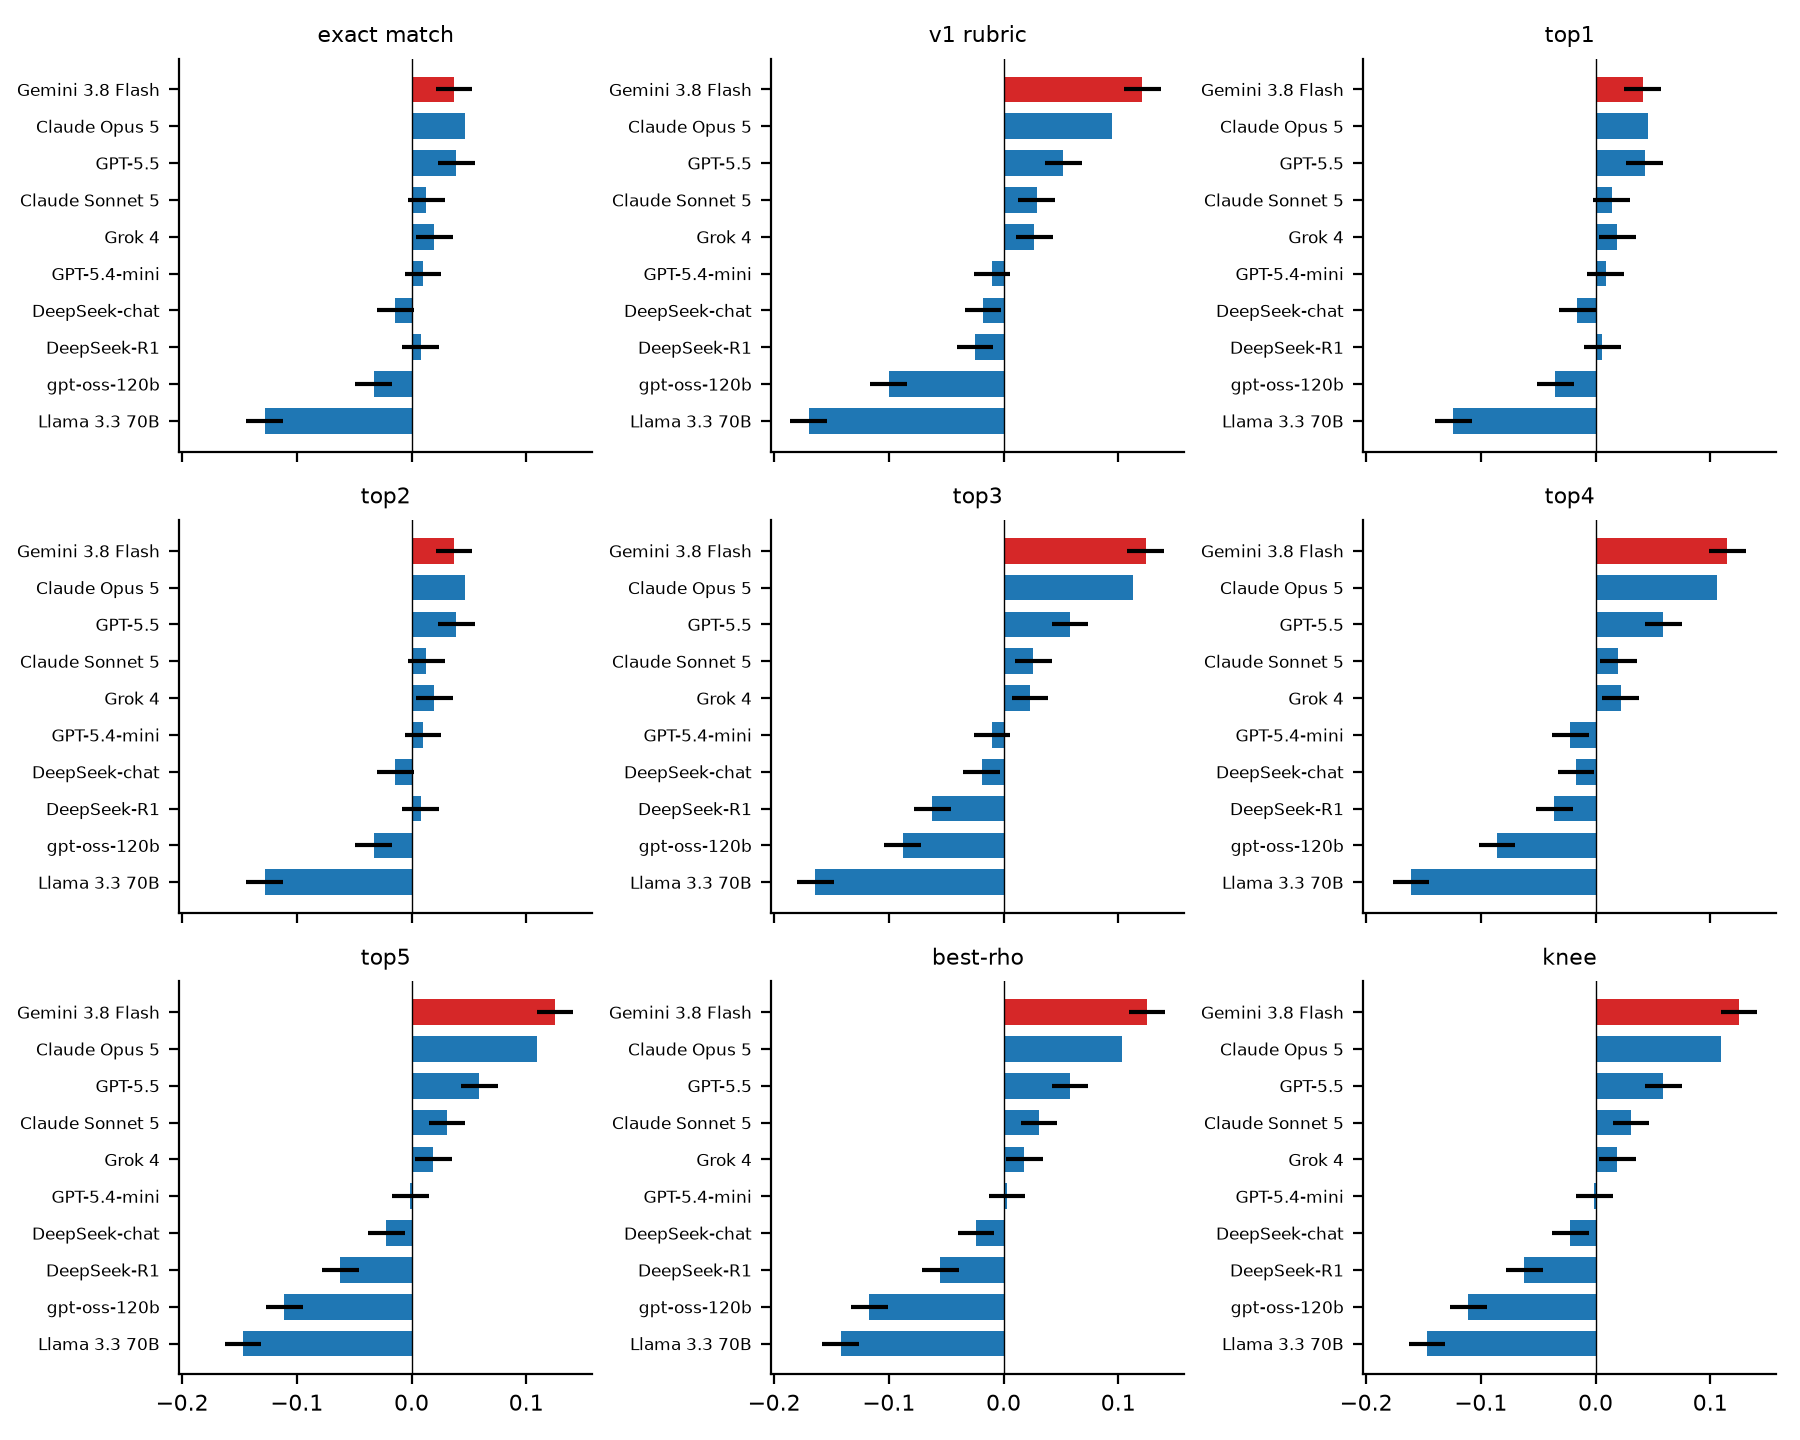
\includegraphics[width=0.9\textwidth]{fig_bt_all_rules.png}\caption{Bradley--Terry strengths ($\pm$ SE vs reference) under every reported rule; models fixed in the headline order.}\label{figall:fig_bt_all_rules}\end{figure}
\begin{figure}[htbp]\centering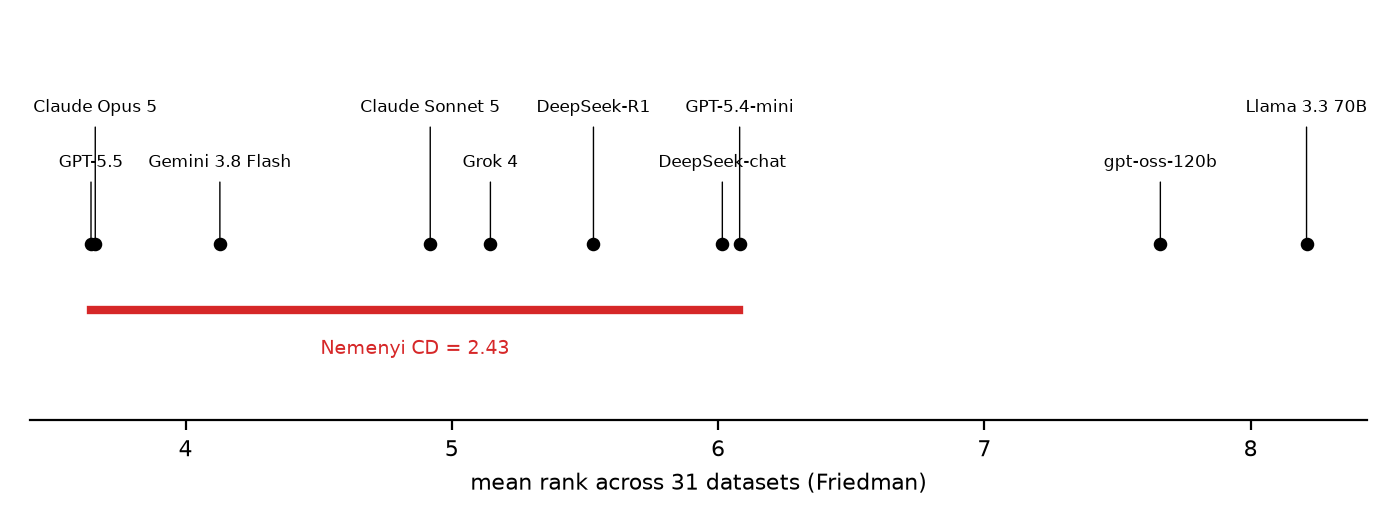
\includegraphics[width=0.9\textwidth]{fig_cd_diagram.png}\caption{Critical-difference view of the Friedman test under the headline rule: mean rank per model and the Nemenyi critical difference at $\alpha=.05$.}\label{figall:fig_cd_diagram}\end{figure}
\begin{figure}[htbp]\centering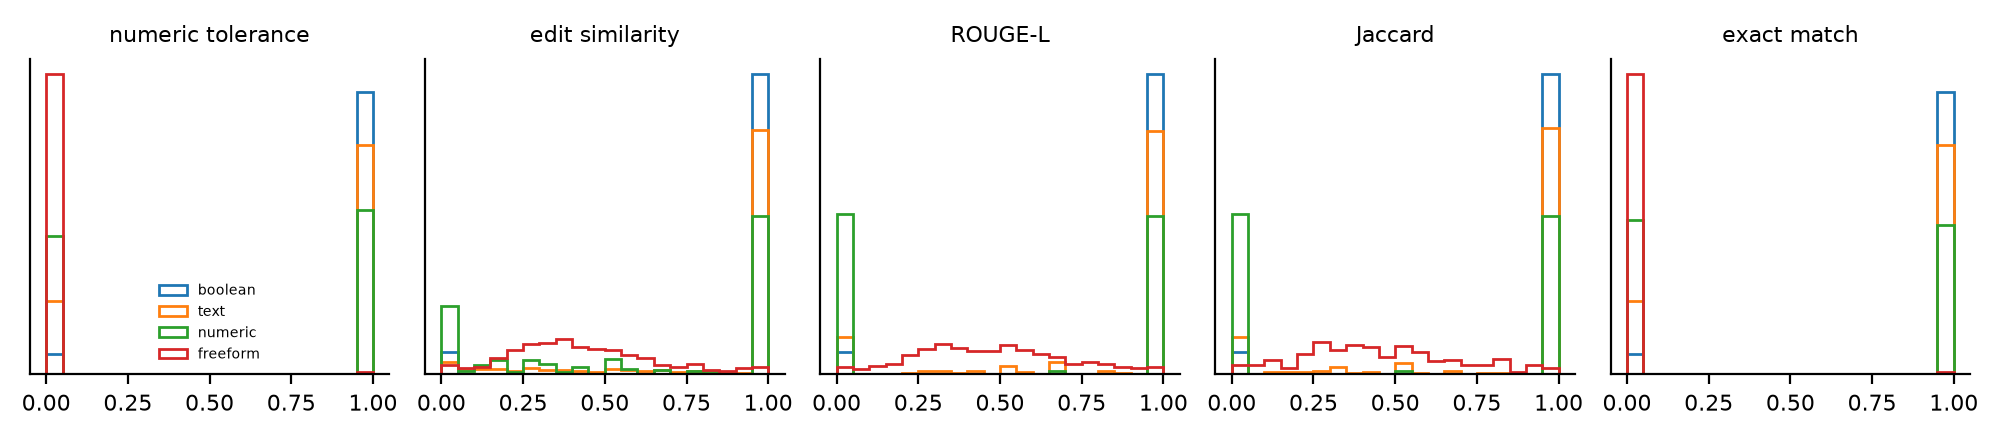
\includegraphics[width=0.9\textwidth]{fig_component_distributions.png}\caption{Distributions of the five components not in v1, by answer type.}\label{figall:fig_component_distributions}\end{figure}
\begin{figure}[htbp]\centering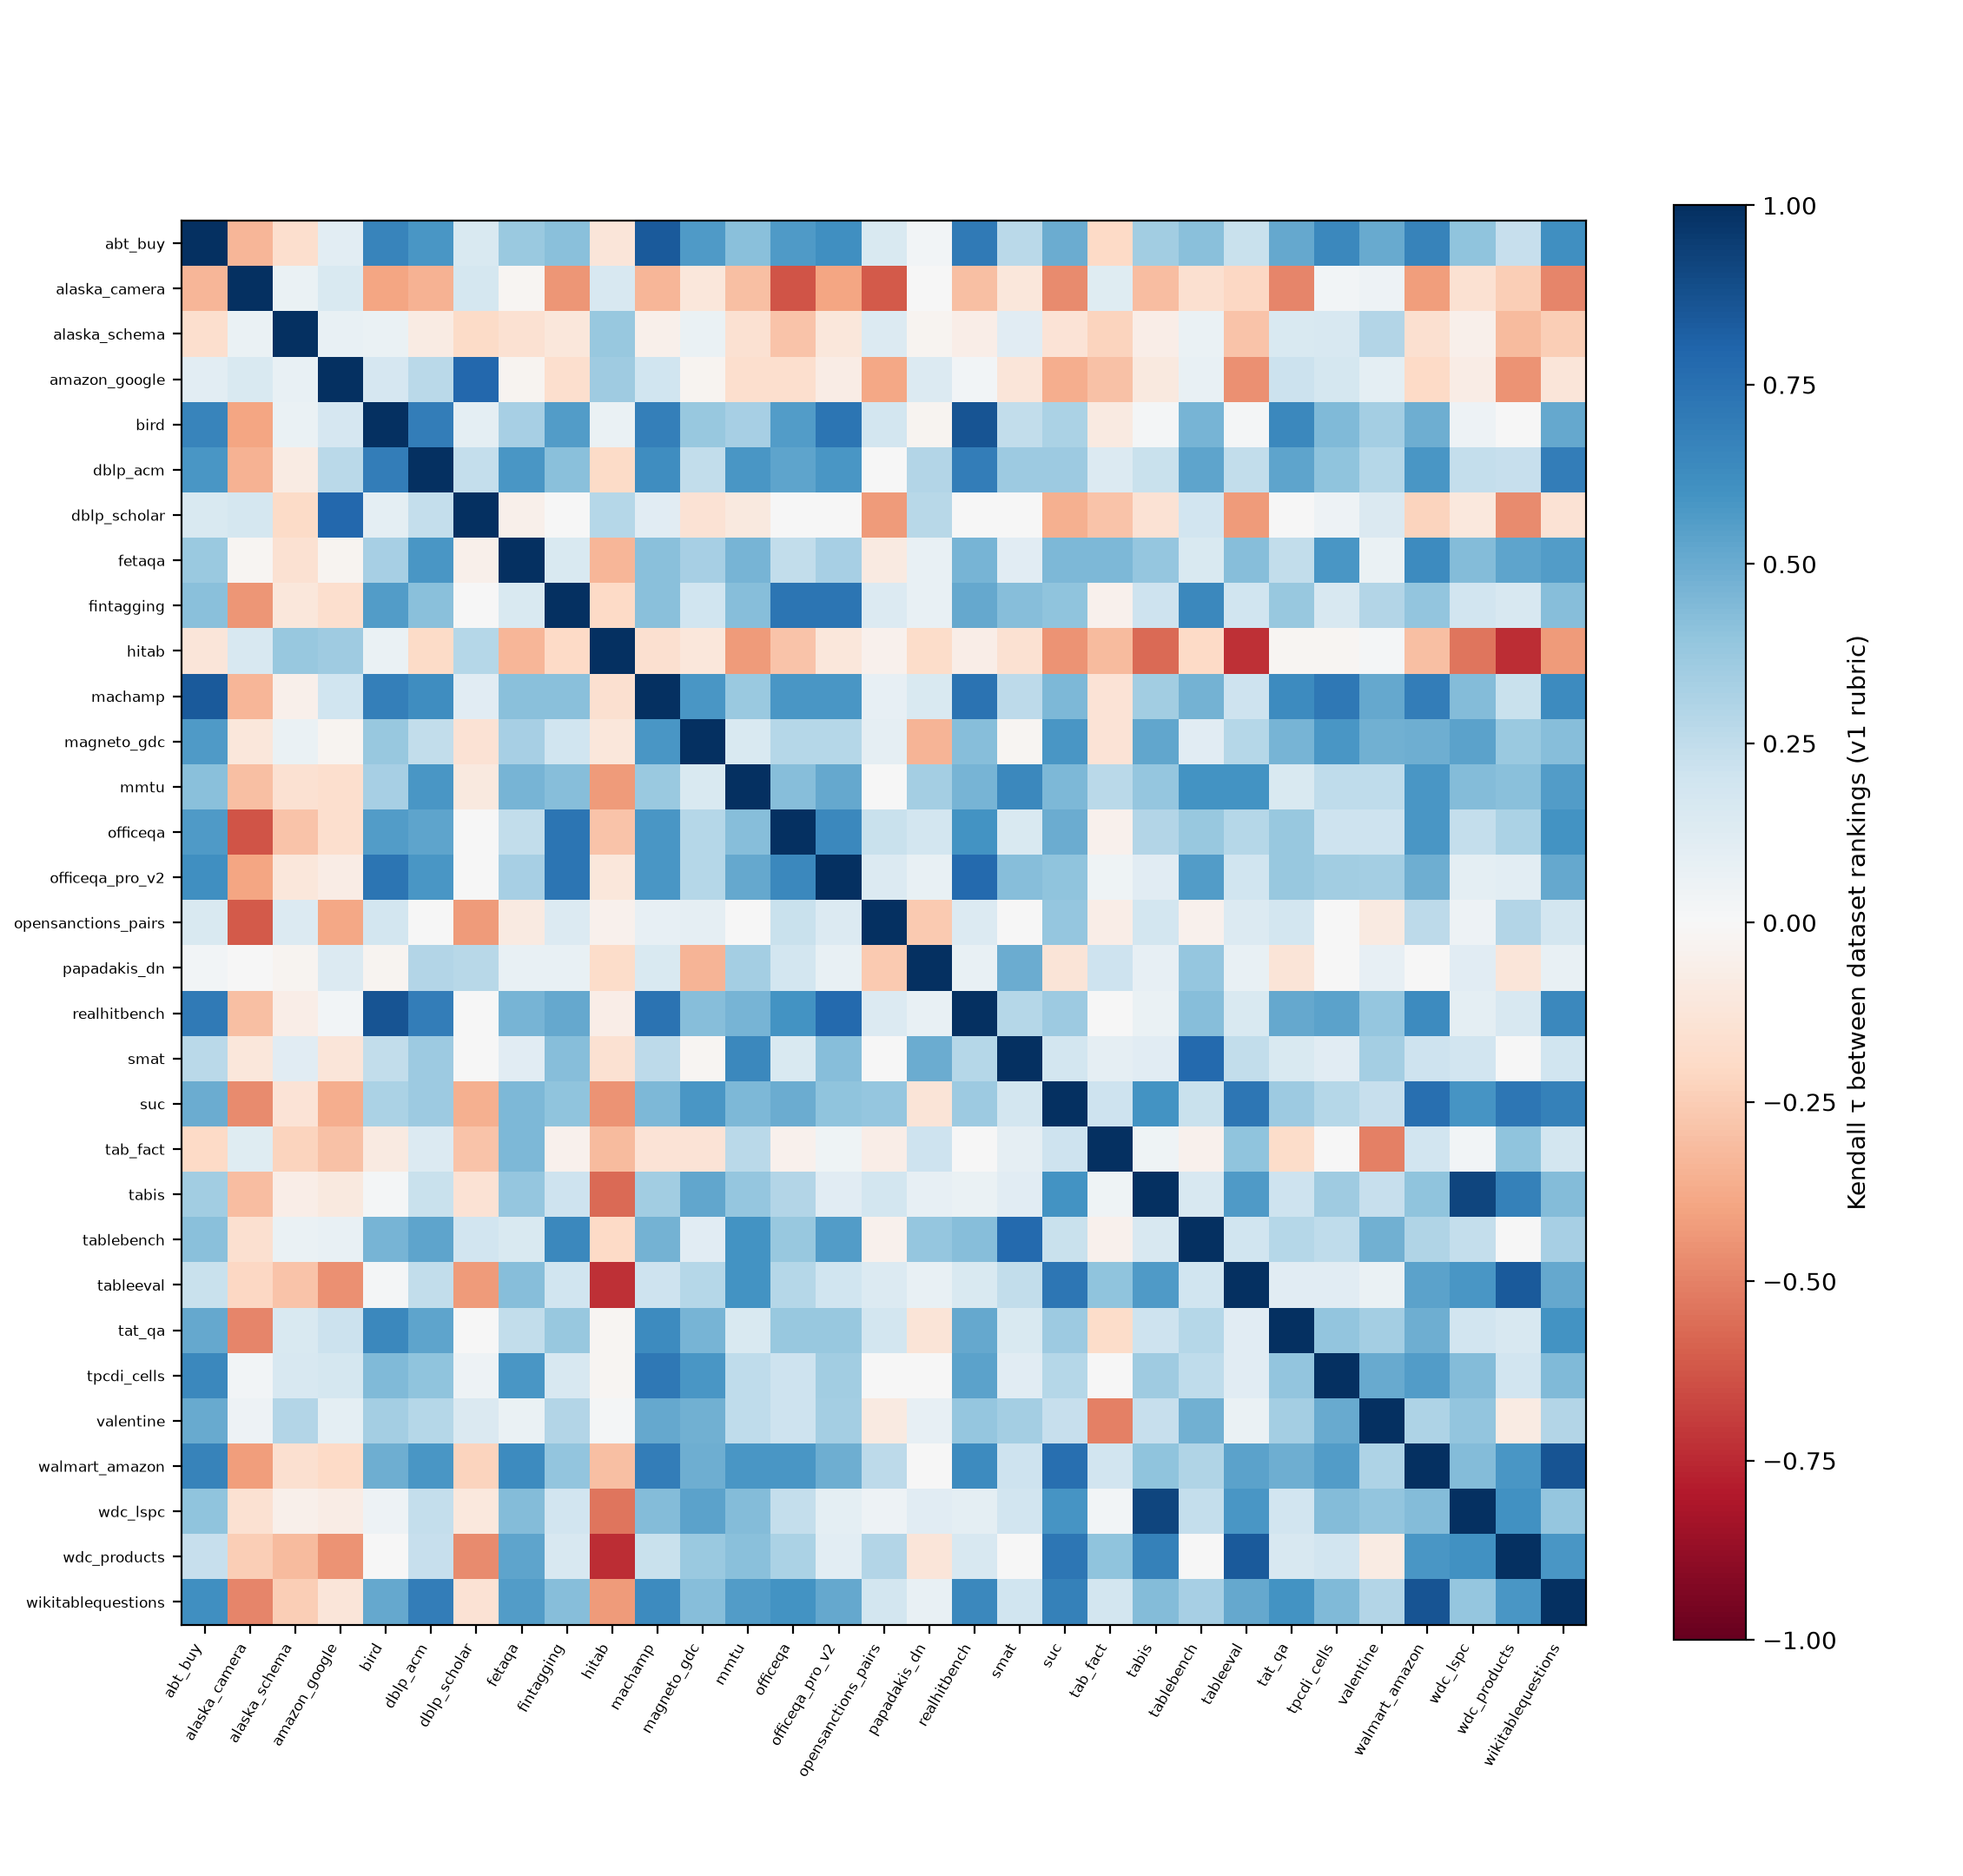
\includegraphics[width=0.9\textwidth]{fig_dataset_tau.png}\caption{Kendall $\tau$ between the model rankings of each pair of datasets under the headline rule.}\label{figall:fig_dataset_tau}\end{figure}
\begin{figure}[htbp]\centering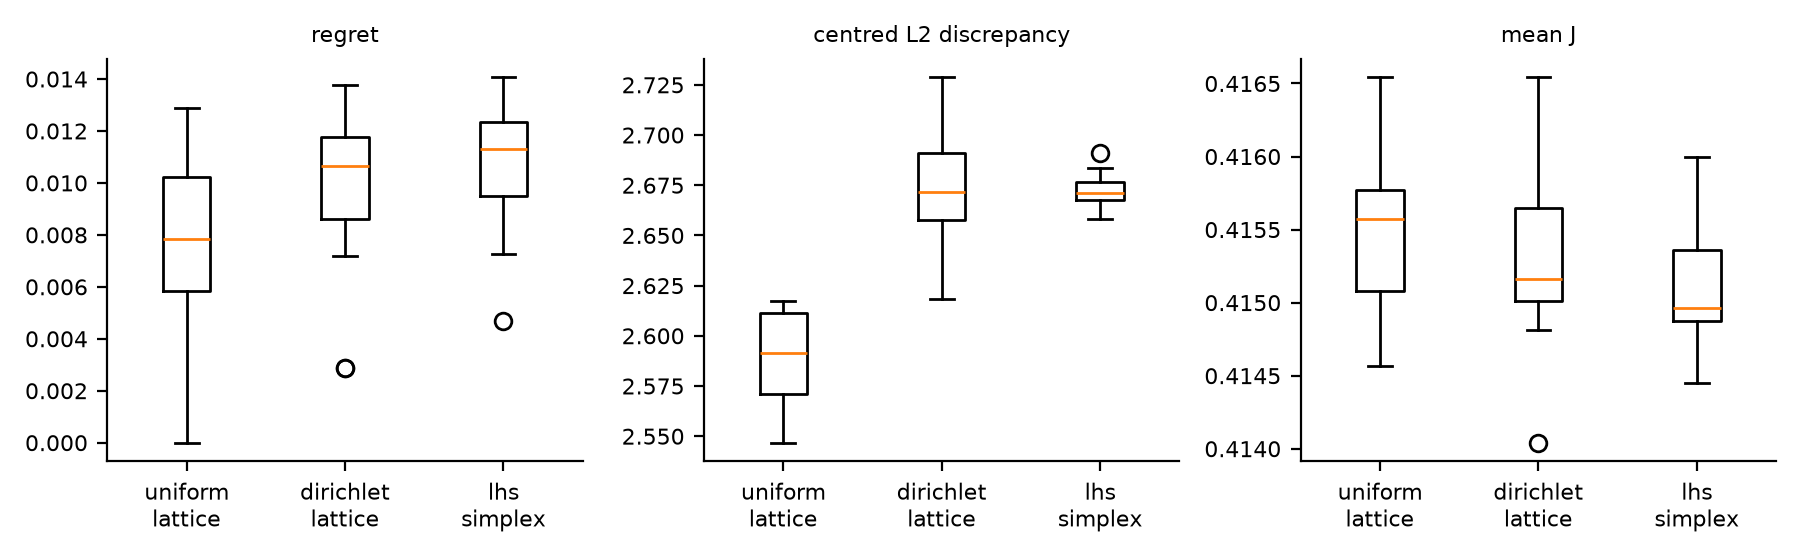
\includegraphics[width=0.9\textwidth]{fig_design_metrics.png}\caption{Sampled designs over 20 seeds: regret against the best over all seeds and designs, centred $L_2$ discrepancy and mean $J$ of the design.}\label{figall:fig_design_metrics}\end{figure}
\begin{figure}[htbp]\centering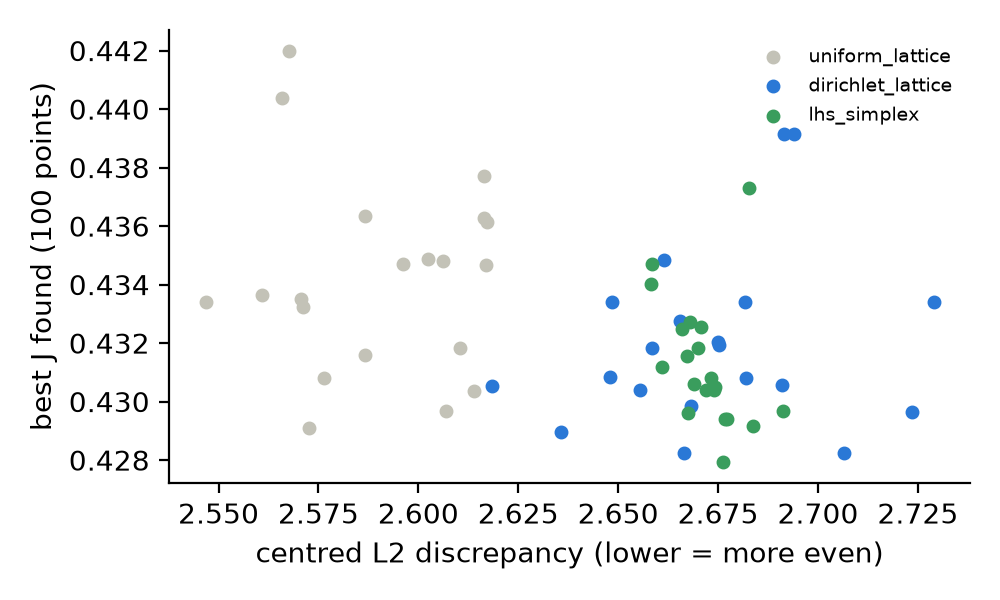
\includegraphics[width=0.9\textwidth]{fig_designs.png}\caption{Sampled designs: best $J$ found per seed.}\label{figall:fig_designs}\end{figure}
\begin{figure}[htbp]\centering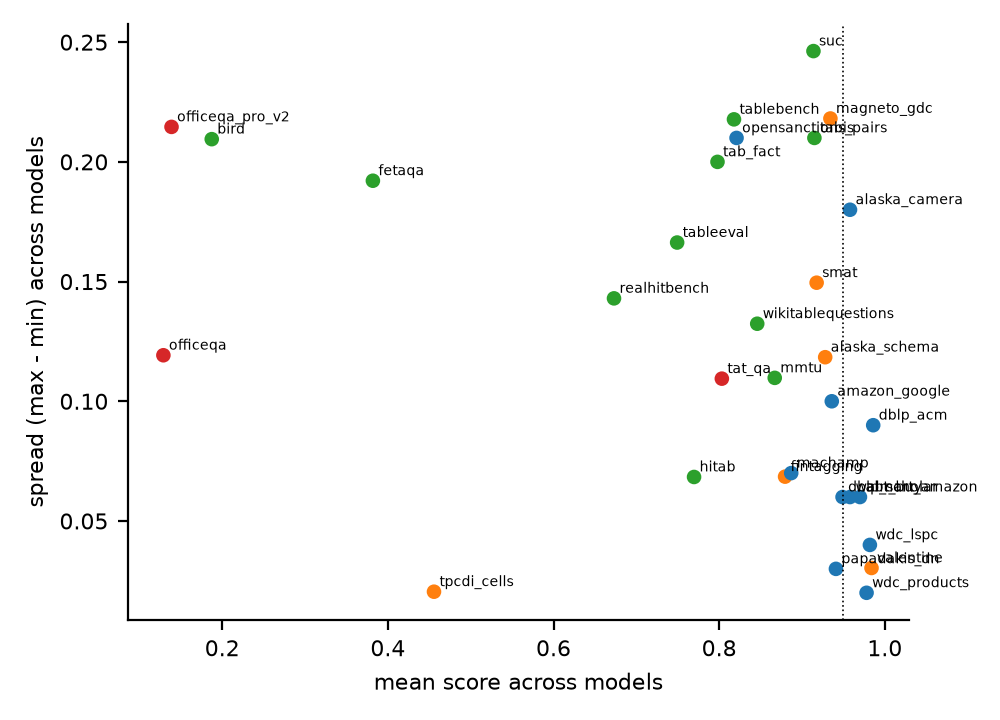
\includegraphics[width=0.9\textwidth]{fig_diagnostics_scatter.png}\caption{Dataset diagnostics: mean score against spread across models; dotted line marks the ceiling flag.}\label{figall:fig_diagnostics_scatter}\end{figure}
\begin{figure}[htbp]\centering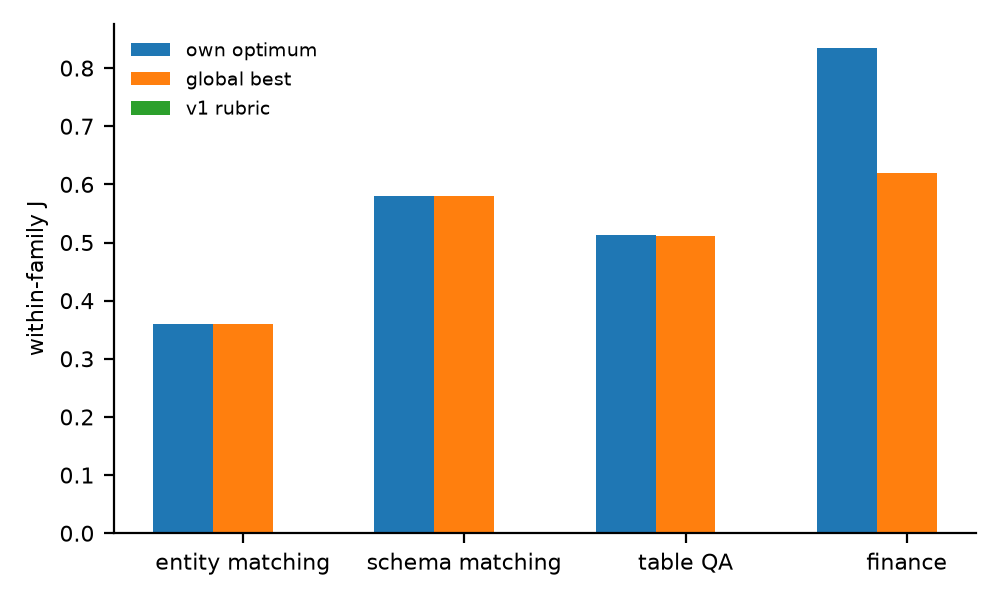
\includegraphics[width=0.9\textwidth]{fig_family_j.png}\caption{Within-family $J$ under each family's own optimum, the global best and the v1 rubric.}\label{figall:fig_family_j}\end{figure}
\begin{figure}[htbp]\centering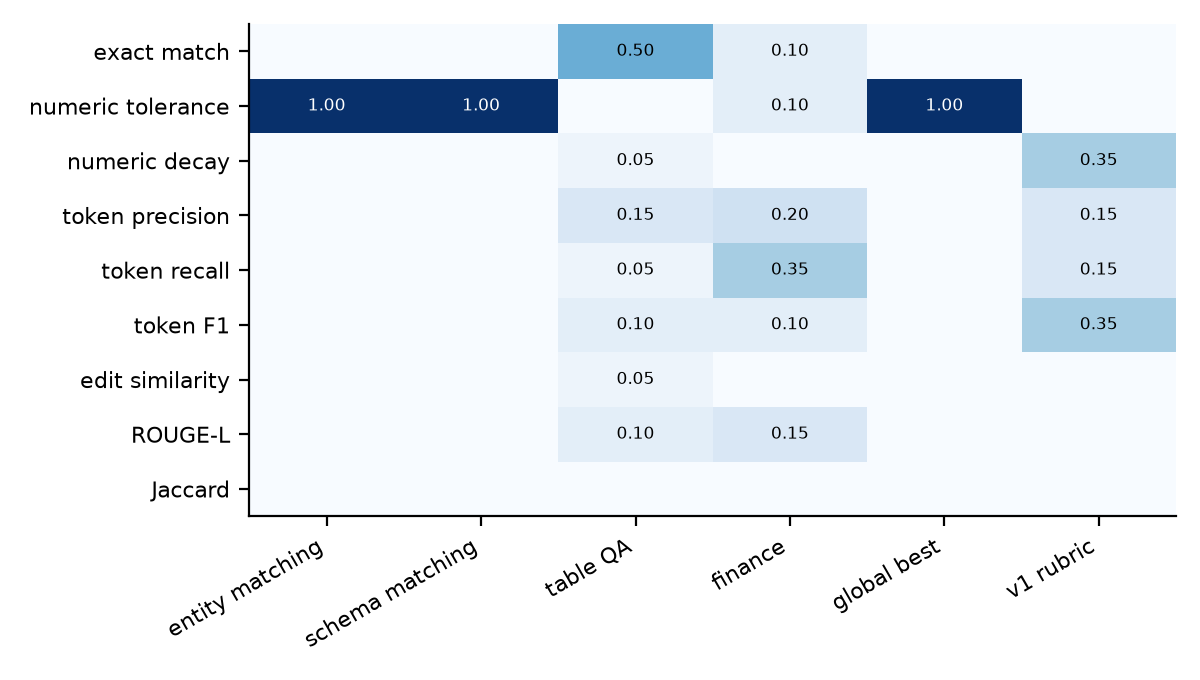
\includegraphics[width=0.9\textwidth]{fig_family_weights.png}\caption{Per-family optimum, global optimum and the v1 rubric over the nine components.}\label{figall:fig_family_weights}\end{figure}
\begin{figure}[htbp]\centering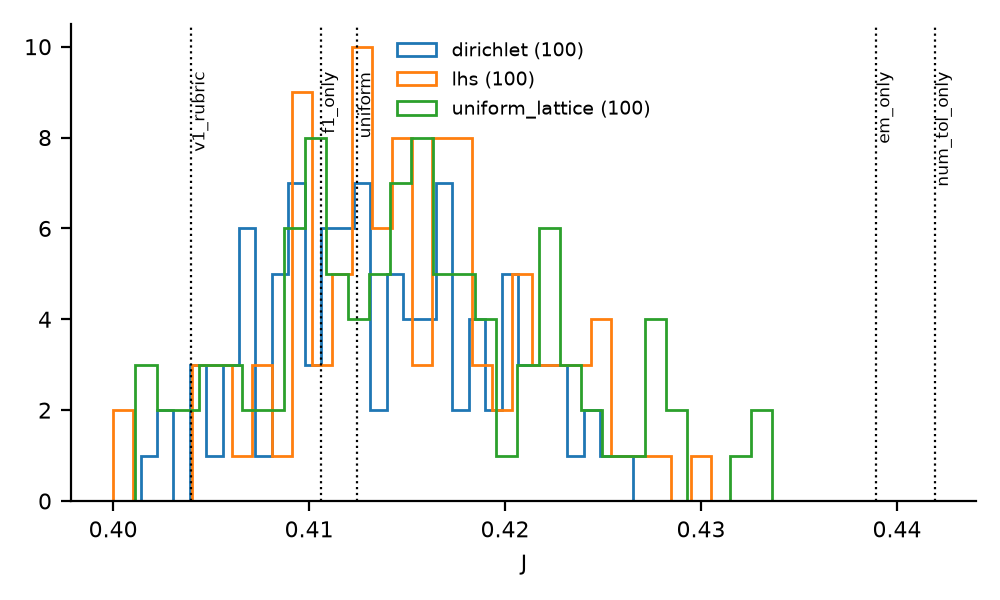
\includegraphics[width=0.9\textwidth]{fig_j_by_design.png}\caption{Distribution of $J$ over the 100 candidates of each design, with the five baselines marked.}\label{figall:fig_j_by_design}\end{figure}
\begin{figure}[htbp]\centering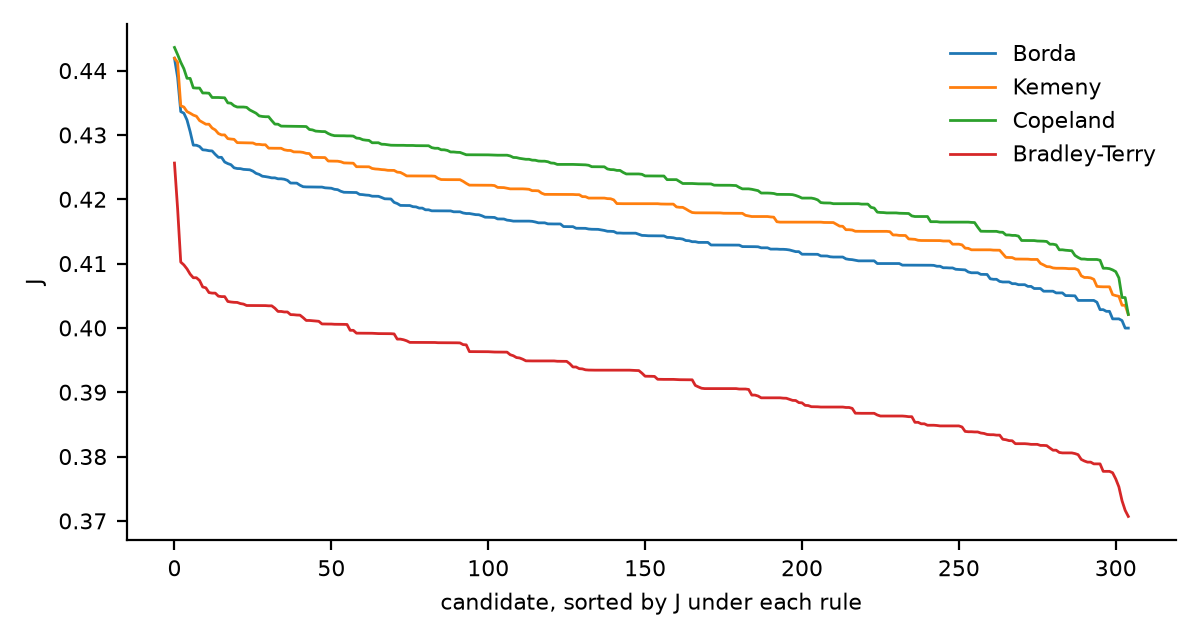
\includegraphics[width=0.9\textwidth]{fig_j_pooling_rules.png}\caption{Objective over all candidates under four pooling rules.}\label{figall:fig_j_pooling_rules}\end{figure}
\begin{figure}[htbp]\centering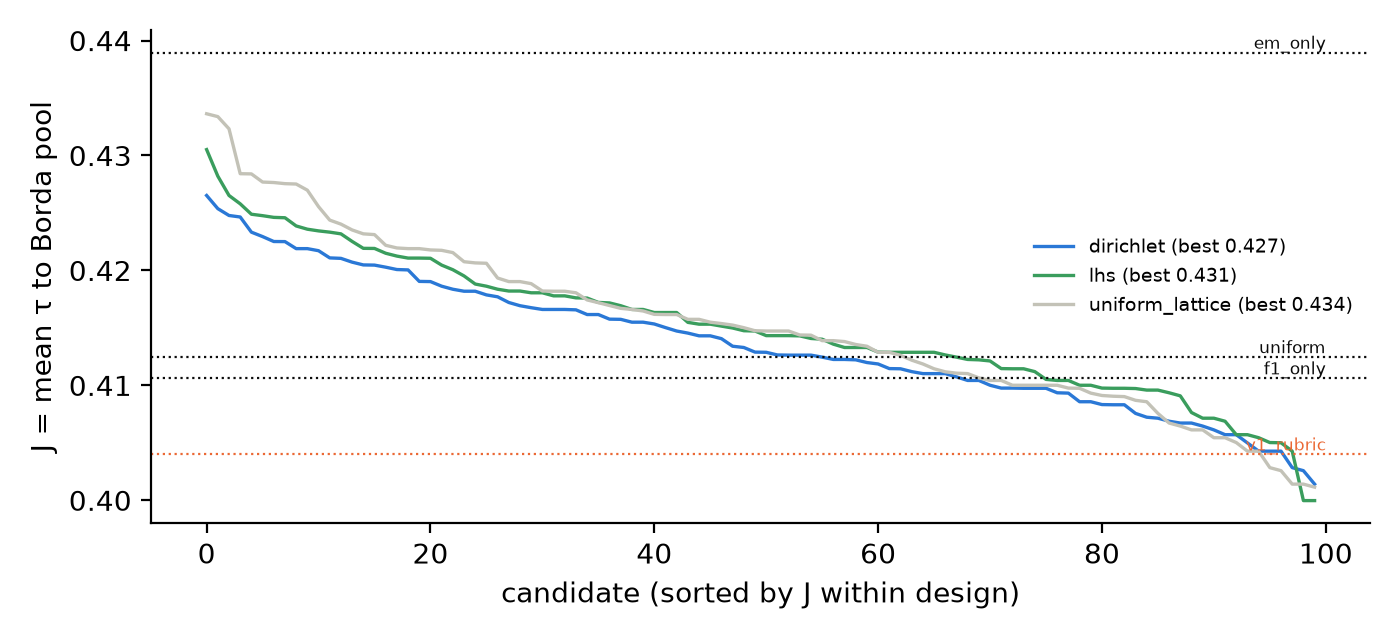
\includegraphics[width=0.9\textwidth]{fig_landscape.png}\caption{All 305 candidates sorted by $J$, with the baselines marked.}\label{figall:fig_landscape}\end{figure}
\begin{figure}[htbp]\centering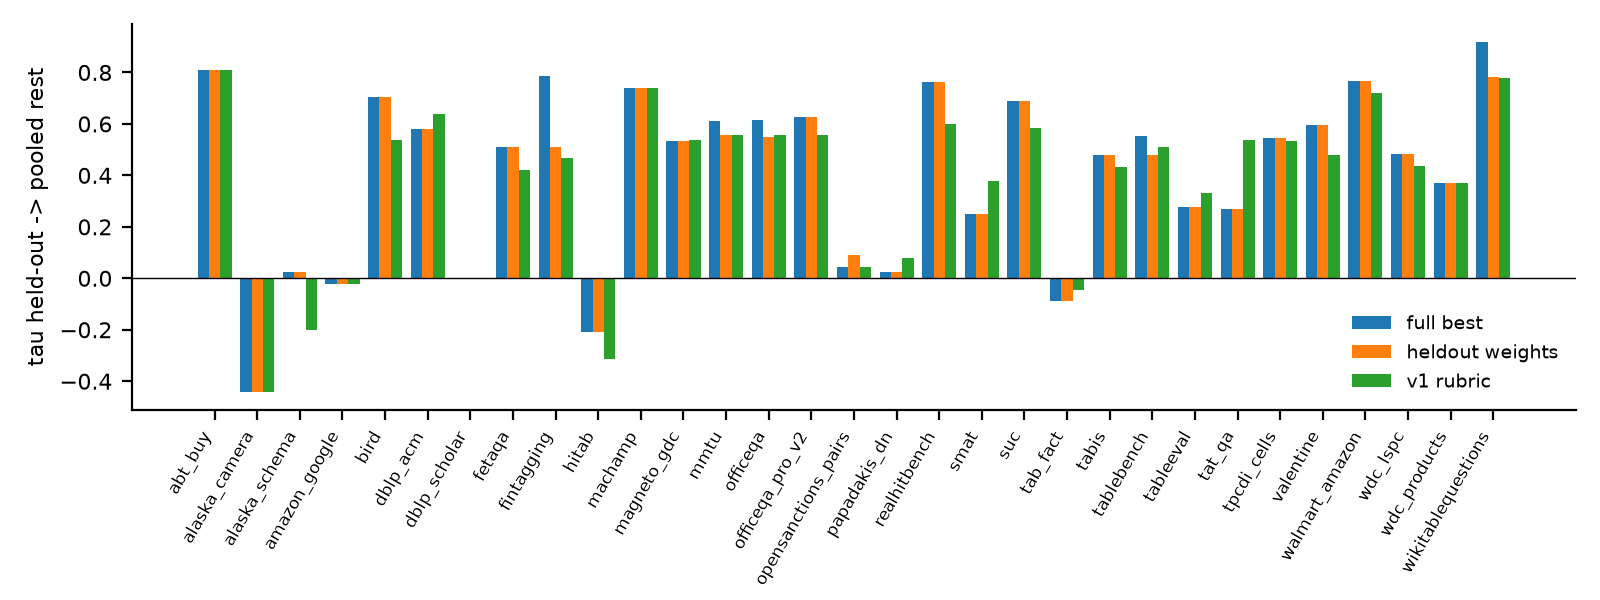
\includegraphics[width=0.9\textwidth]{fig_lodo_tau.png}\caption{Leave-one-dataset-out: agreement of the held-out dataset with the pooled rest under re-fitted weights, the full best and the v1 rubric.}\label{figall:fig_lodo_tau}\end{figure}
\begin{figure}[htbp]\centering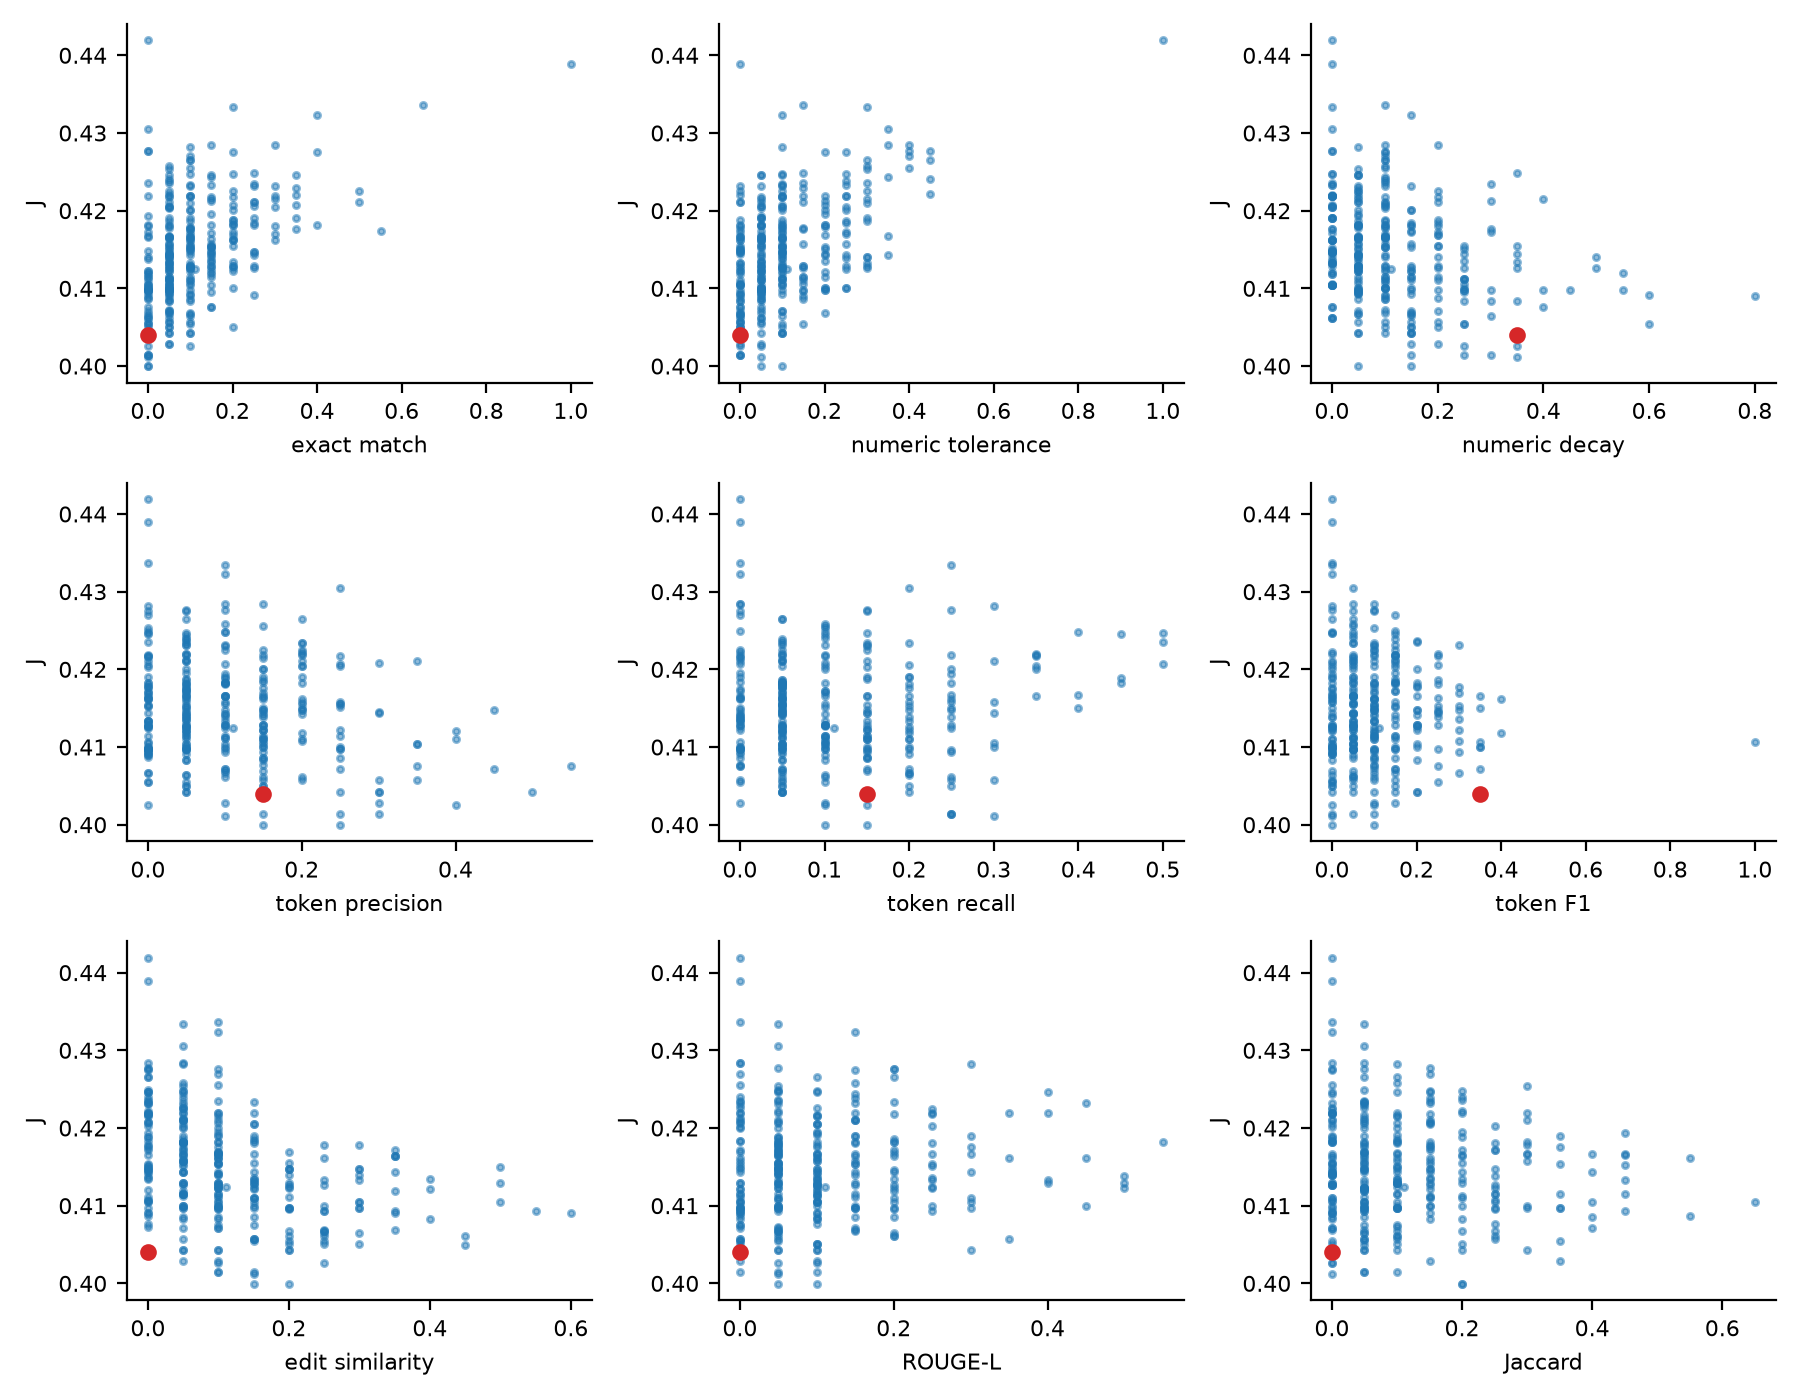
\includegraphics[width=0.9\textwidth]{fig_marginals.png}\caption{$J$ against each component weight over all candidates; red = v1 rubric.}\label{figall:fig_marginals}\end{figure}
\begin{figure}[htbp]\centering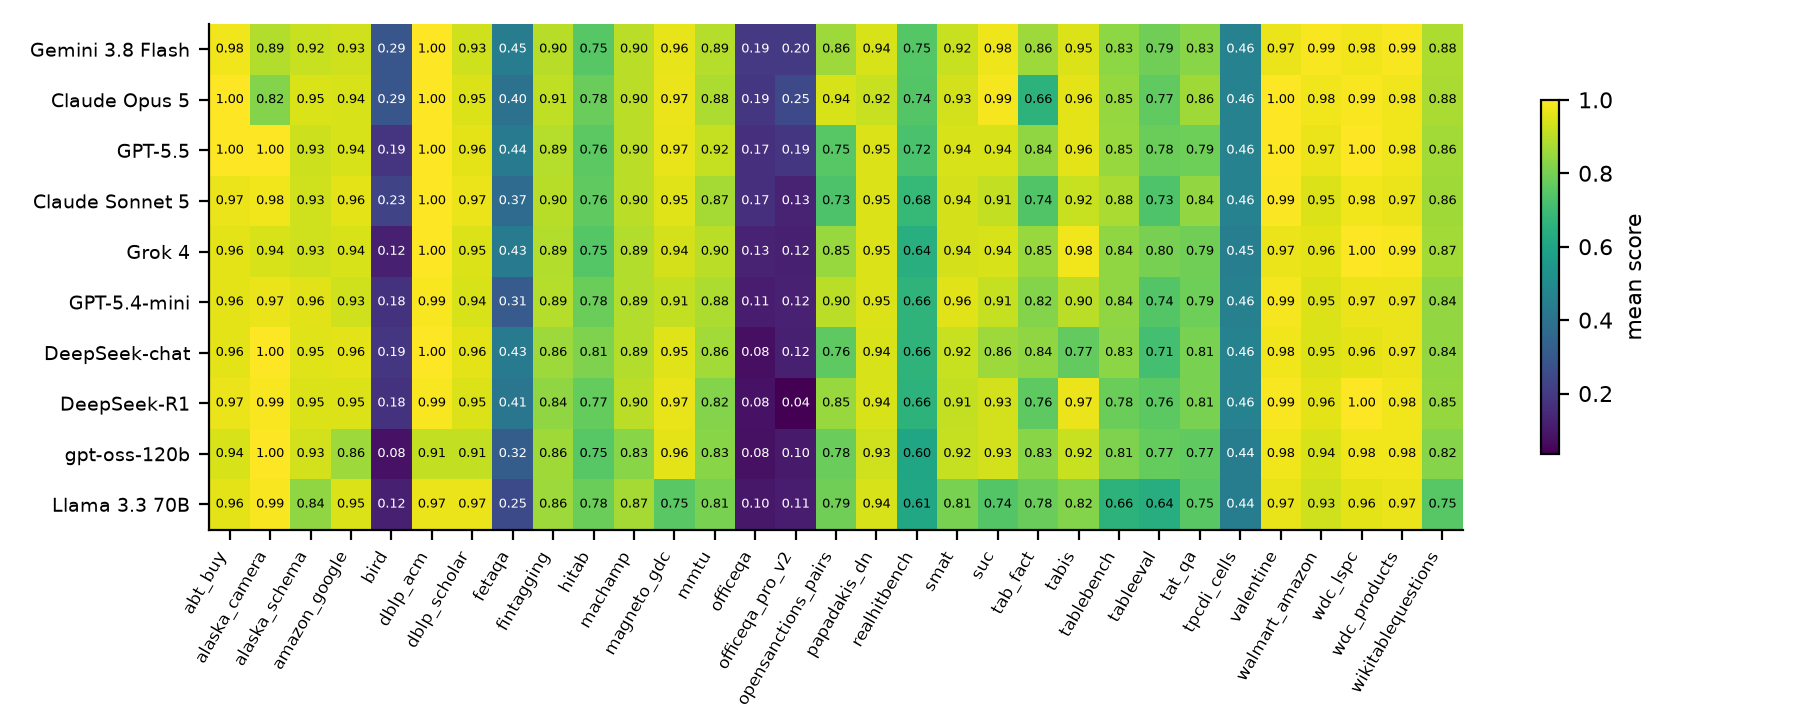
\includegraphics[width=0.9\textwidth]{fig_model_dataset_heatmap.png}\caption{Mean score per model and dataset under the headline rule.}\label{figall:fig_model_dataset_heatmap}\end{figure}
\begin{figure}[htbp]\centering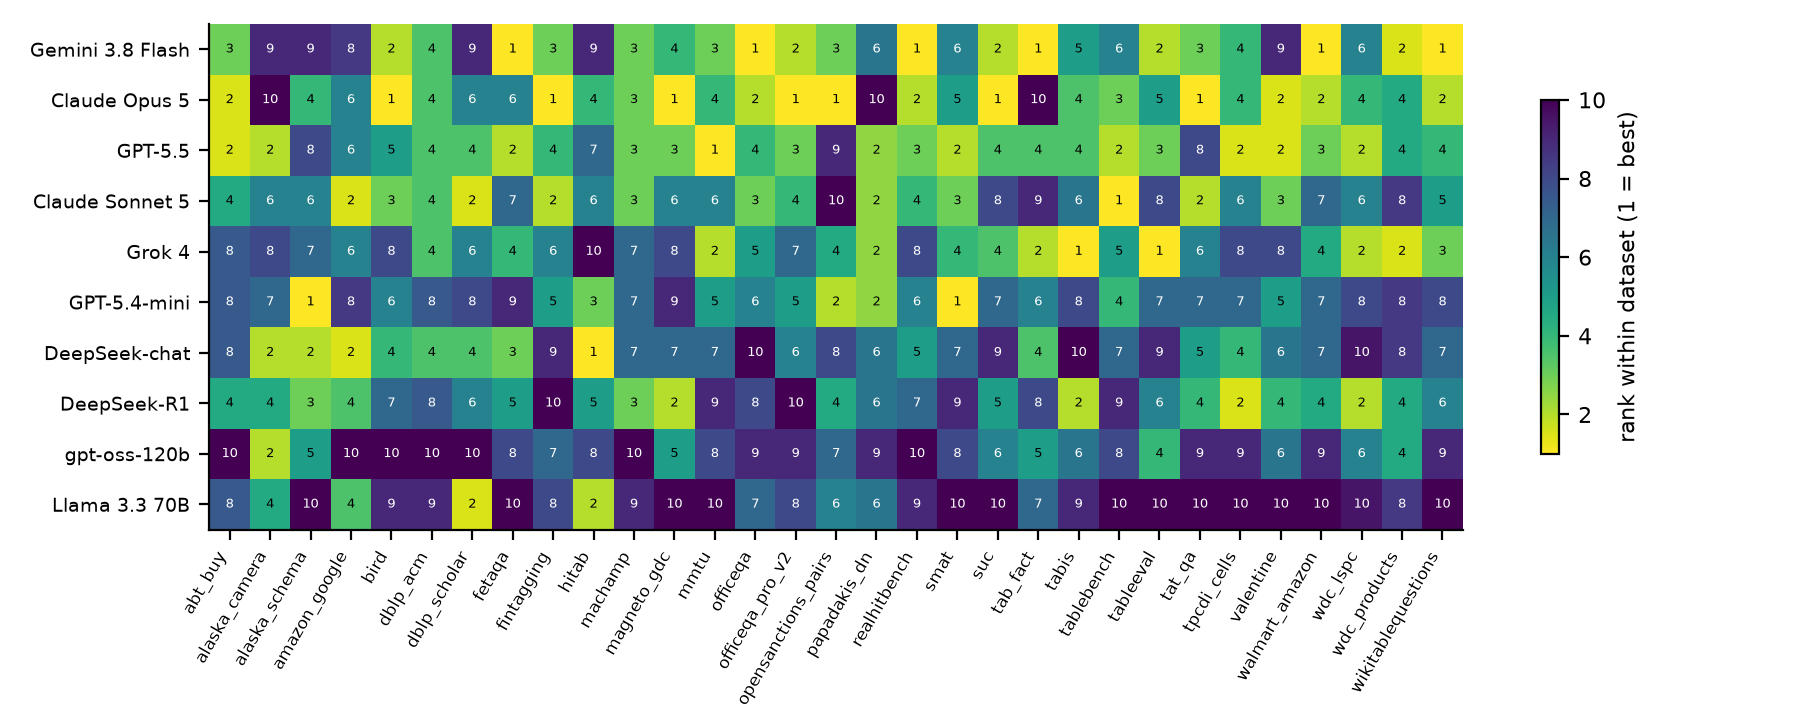
\includegraphics[width=0.9\textwidth]{fig_model_dataset_ranks.png}\caption{Rank per model and dataset under the headline rule.}\label{figall:fig_model_dataset_ranks}\end{figure}
\begin{figure}[htbp]\centering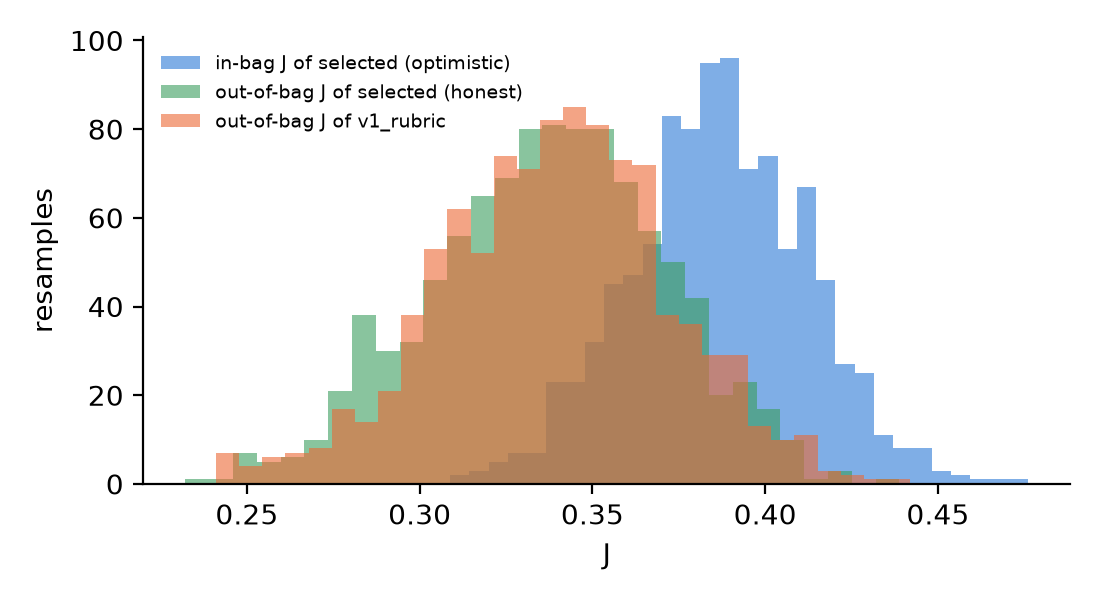
\includegraphics[width=0.9\textwidth]{fig_nested.png}\caption{In-bag vs out-of-bag $J$ of the selected candidate against the v1 rubric.}\label{figall:fig_nested}\end{figure}
\begin{figure}[htbp]\centering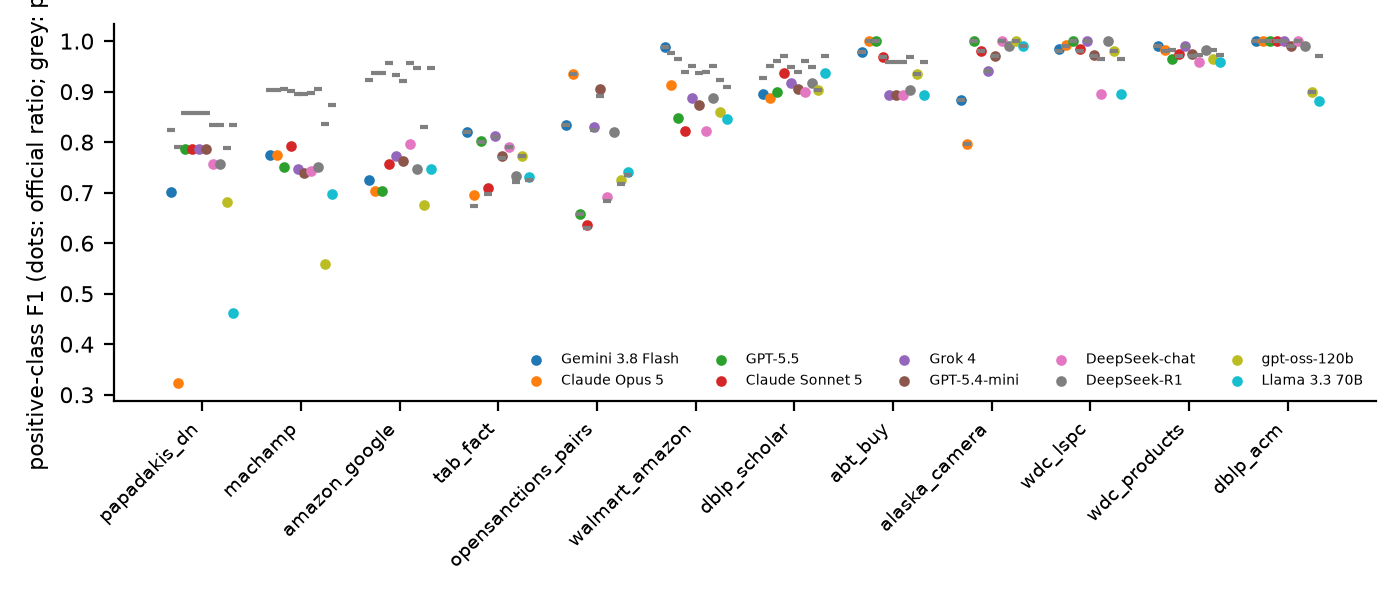
\includegraphics[width=0.9\textwidth]{fig_official_f1_models.png}\caption{Positive-class F1 on the balanced pool (grey) and at the official match ratio (coloured) per model and matching dataset.}\label{figall:fig_official_f1_models}\end{figure}
\begin{figure}[htbp]\centering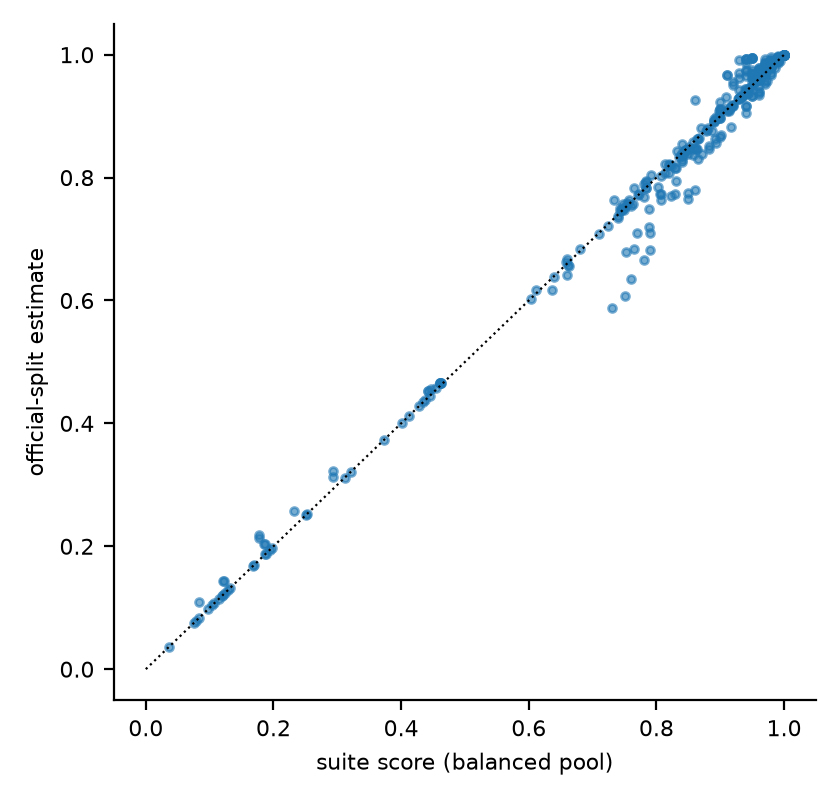
\includegraphics[width=0.9\textwidth]{fig_official_scatter.png}\caption{Suite score against post-stratified official-split estimate for every (dataset, model) pair under the headline rule.}\label{figall:fig_official_scatter}\end{figure}
\begin{figure}[htbp]\centering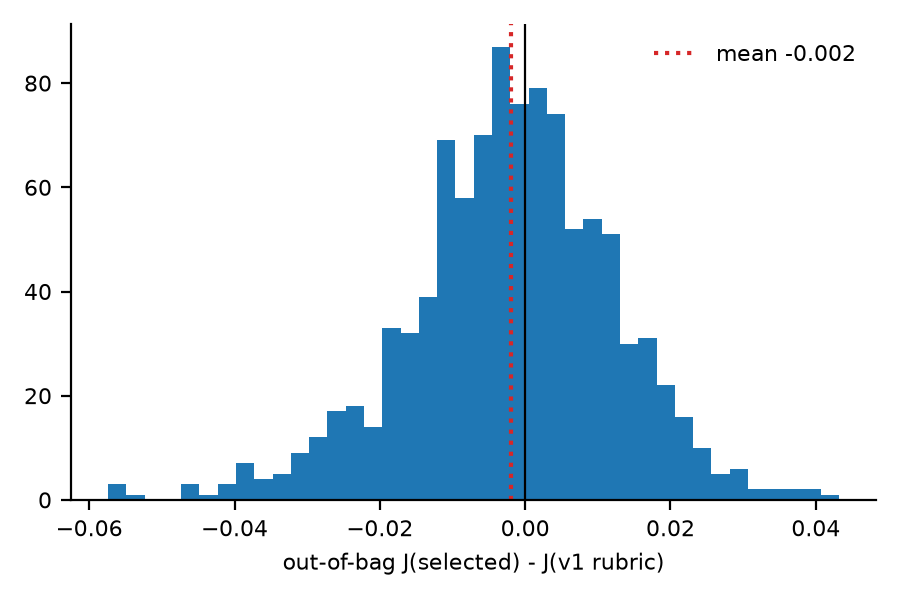
\includegraphics[width=0.9\textwidth]{fig_oob_difference.png}\caption{Paired out-of-bag difference between the selected candidate and the v1 rubric over 1,000 resamples.}\label{figall:fig_oob_difference}\end{figure}
\begin{figure}[htbp]\centering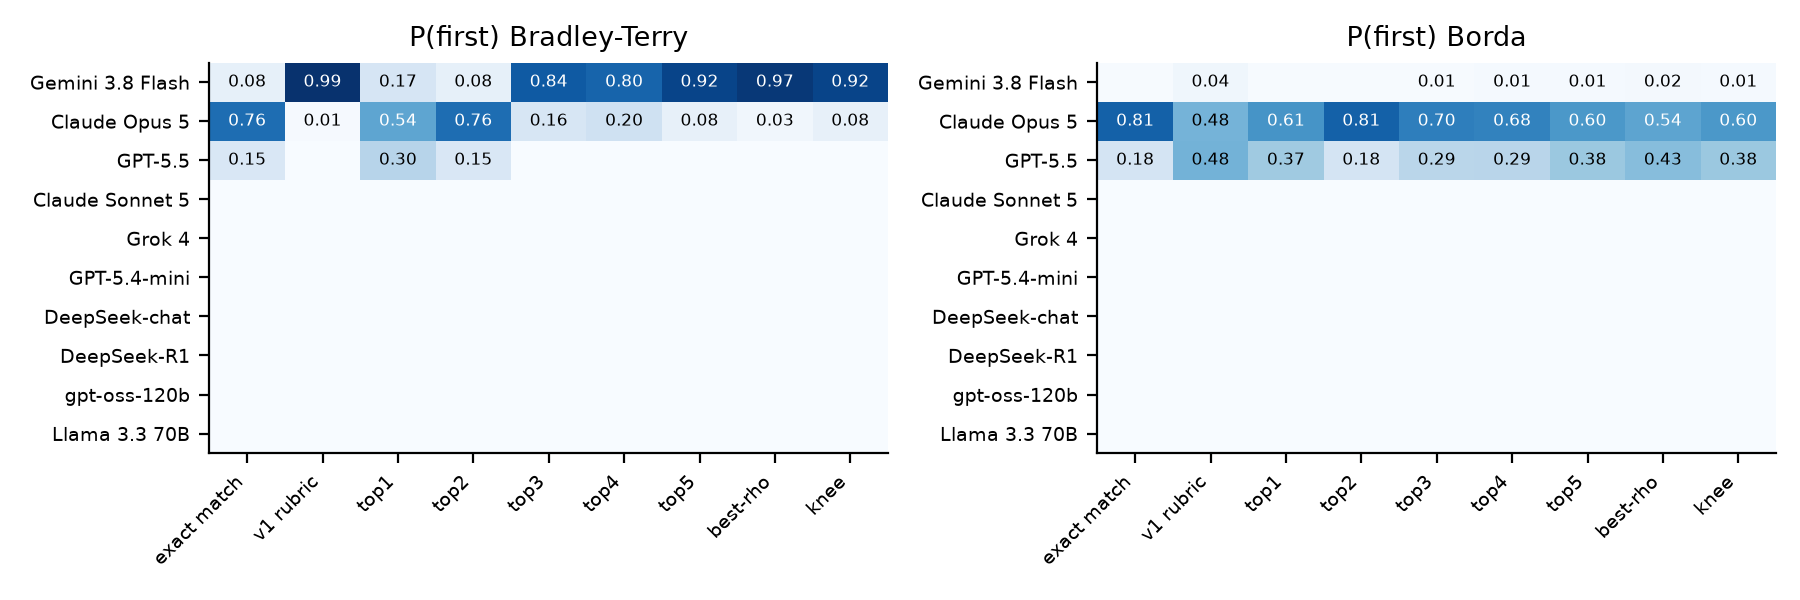
\includegraphics[width=0.9\textwidth]{fig_p_first.png}\caption{Bootstrap probability of first place under every rule, by pooling method.}\label{figall:fig_p_first}\end{figure}
\begin{figure}[htbp]\centering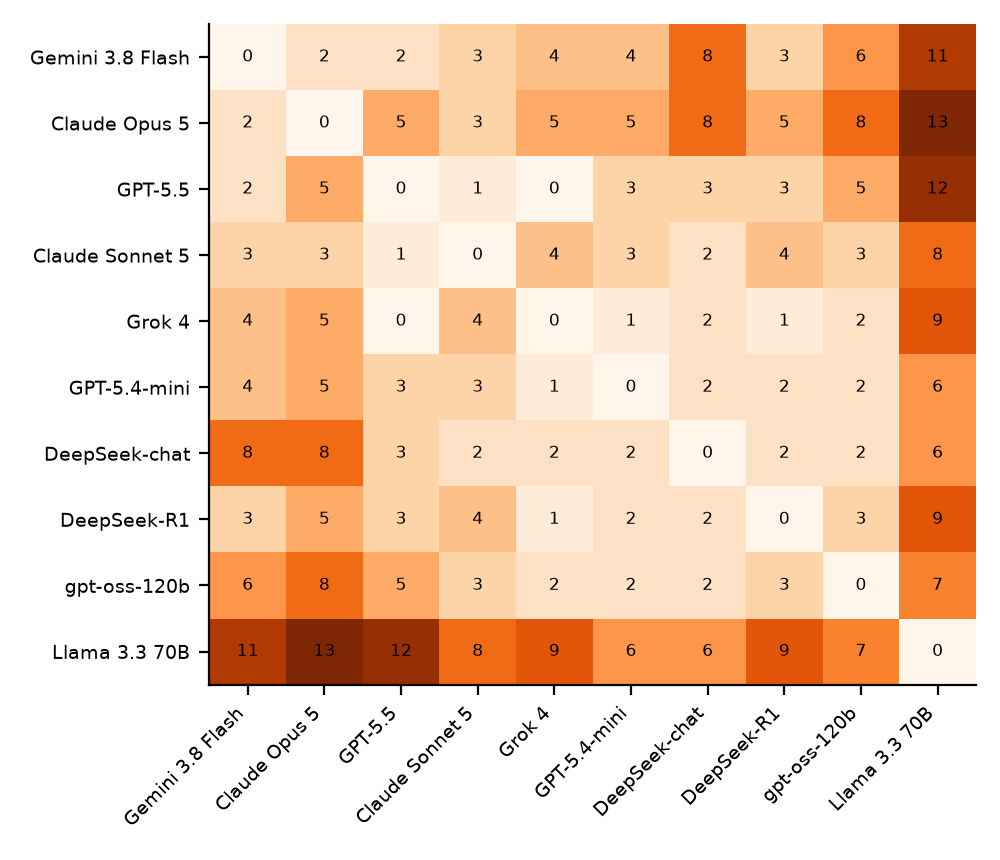
\includegraphics[width=0.9\textwidth]{fig_pairwise_significance.png}\caption{Number of datasets (of 31) in which the per-item paired test separates each pair of models under the headline rule (Holm within dataset).}\label{figall:fig_pairwise_significance}\end{figure}
\begin{figure}[htbp]\centering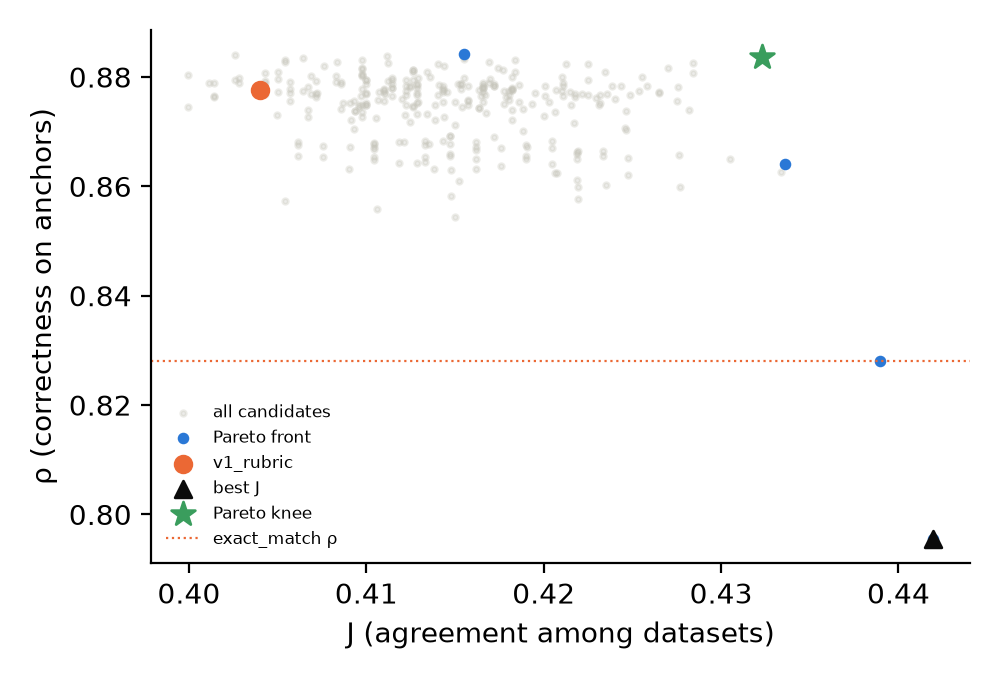
\includegraphics[width=0.9\textwidth]{fig_pareto.png}\caption{Agreement $J$ against anchor correctness $\rho$ for every candidate.}\label{figall:fig_pareto}\end{figure}
\begin{figure}[htbp]\centering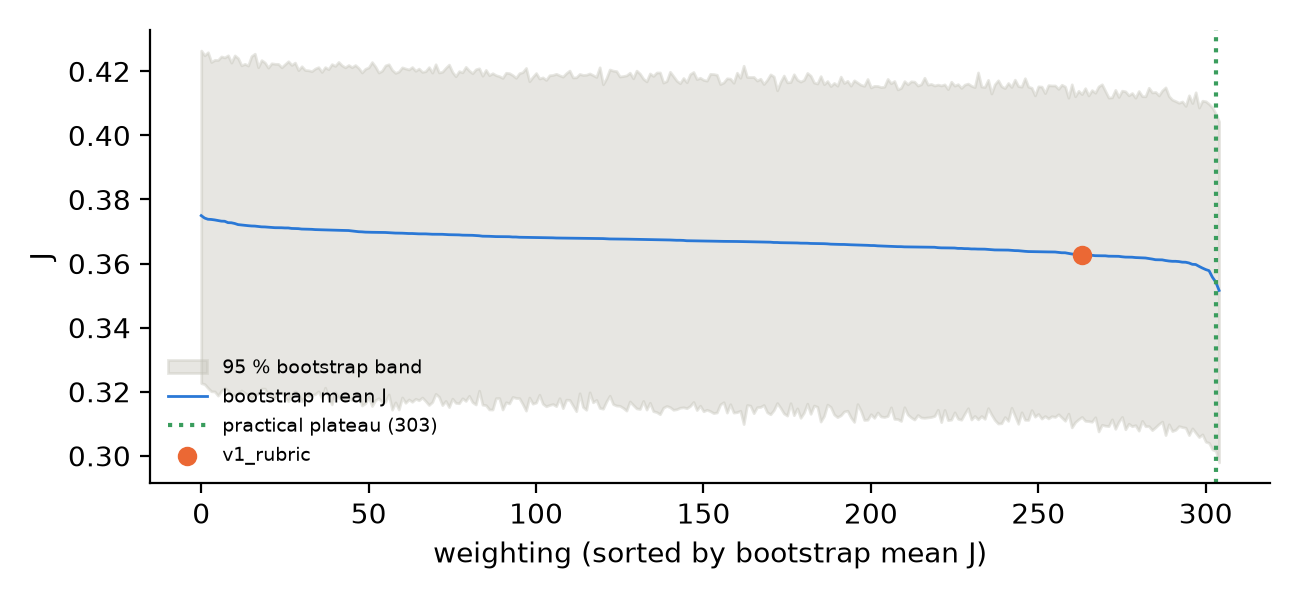
\includegraphics[width=0.9\textwidth]{fig_plateau.png}\caption{Bootstrap band over sorted candidates and the plateau boundary.}\label{figall:fig_plateau}\end{figure}
\begin{figure}[htbp]\centering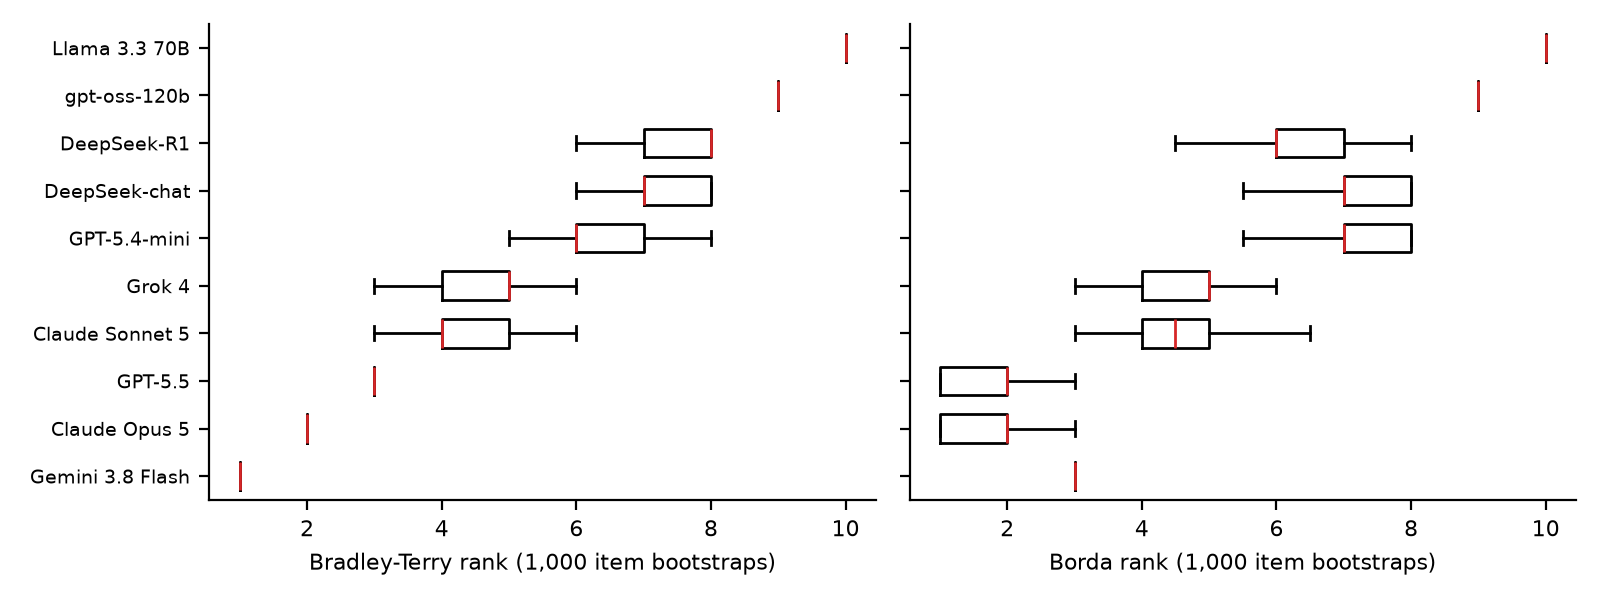
\includegraphics[width=0.9\textwidth]{fig_rank_bootstrap.png}\caption{Bootstrap distribution of each model's rank under the headline rule (v1 rubric).}\label{figall:fig_rank_bootstrap}\end{figure}
\begin{figure}[htbp]\centering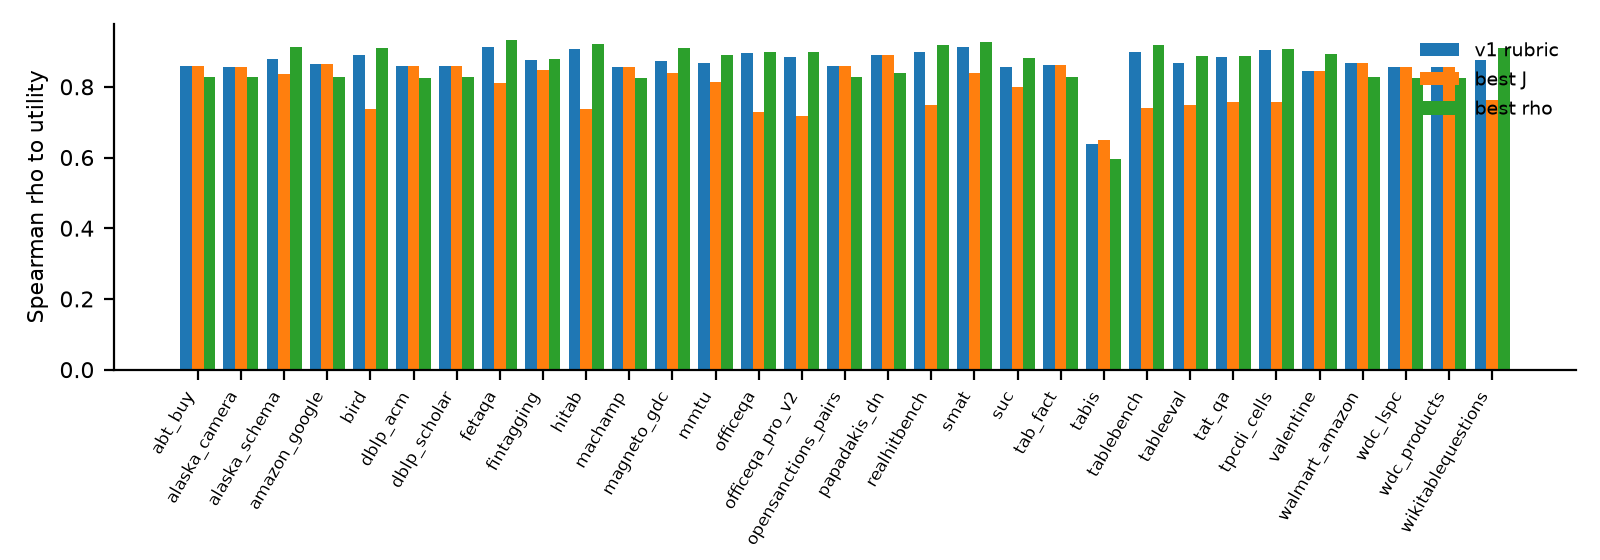
\includegraphics[width=0.9\textwidth]{fig_rho_per_dataset.png}\caption{Anchor correctness per dataset under the v1 rubric, the best-$J$ and the best-$\rho$ candidates.}\label{figall:fig_rho_per_dataset}\end{figure}
\begin{figure}[htbp]\centering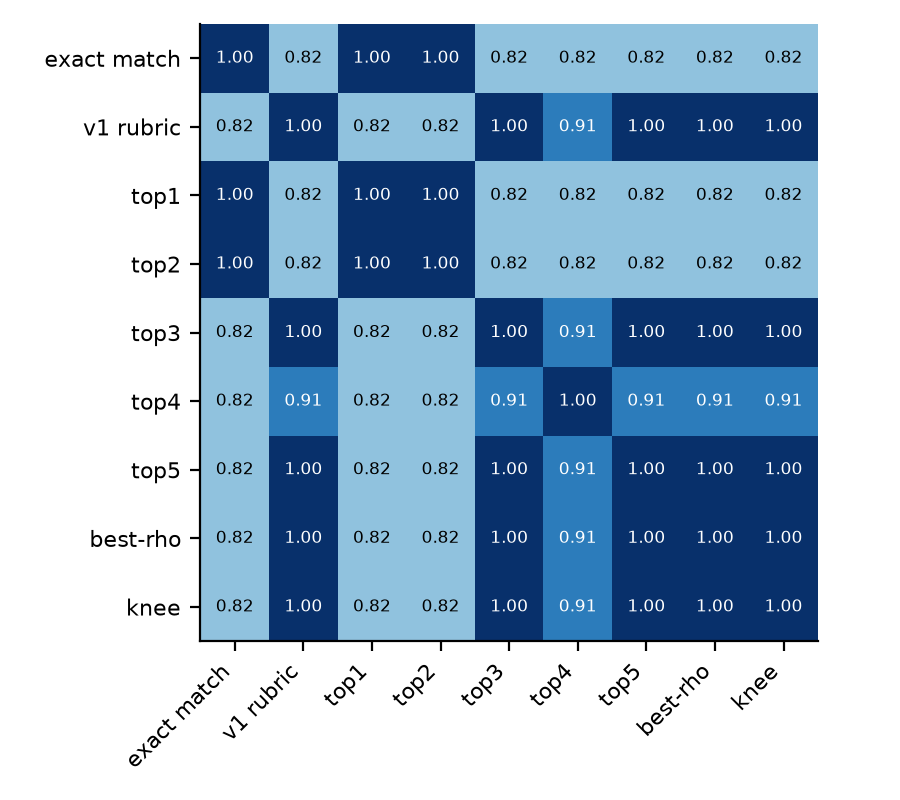
\includegraphics[width=0.9\textwidth]{fig_rule_agreement.png}\caption{Kendall $\tau$ between the Bradley--Terry rankings of each pair of rules.}\label{figall:fig_rule_agreement}\end{figure}
\begin{figure}[htbp]\centering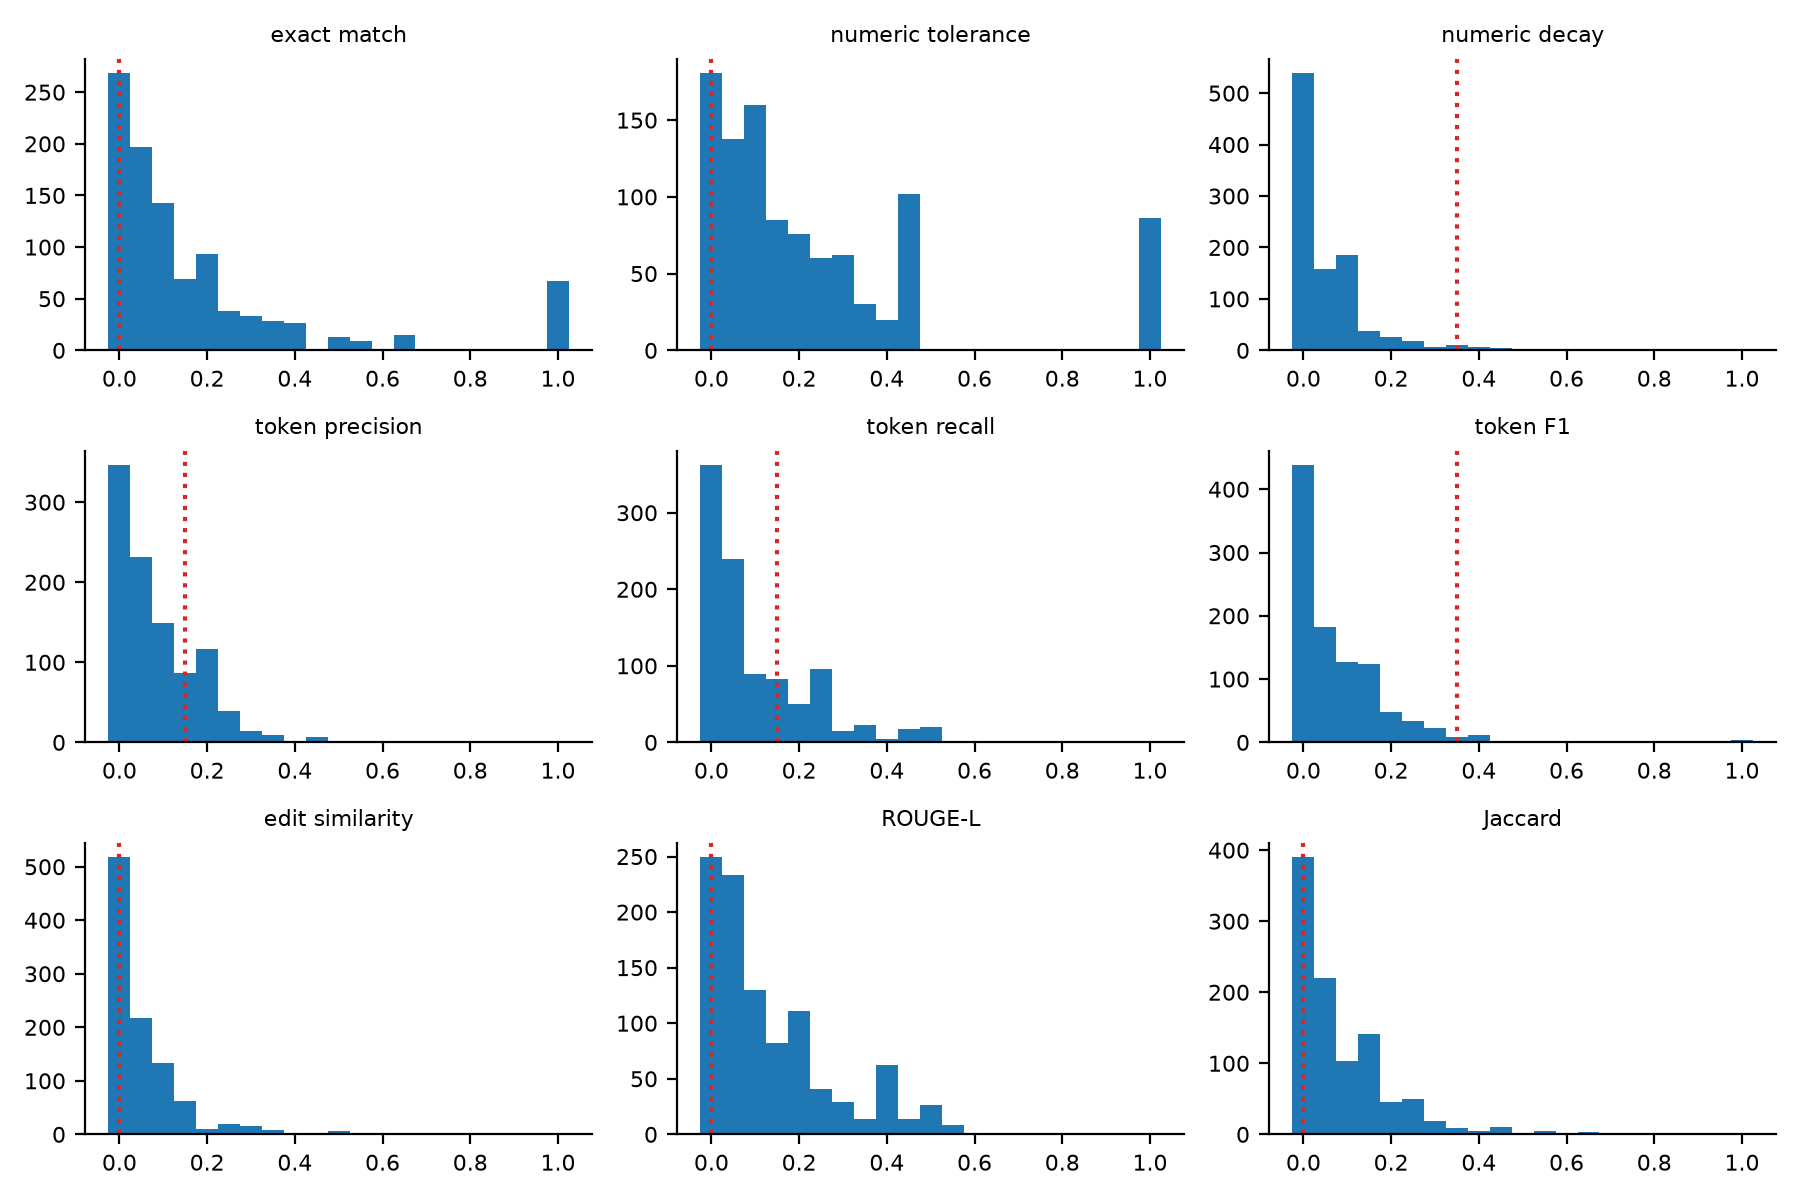
\includegraphics[width=0.9\textwidth]{fig_selected_weights.png}\caption{Weights selected as in-bag best across 1,000 bootstrap resamples; dotted = v1 rubric.}\label{figall:fig_selected_weights}\end{figure}
\begin{figure}[htbp]\centering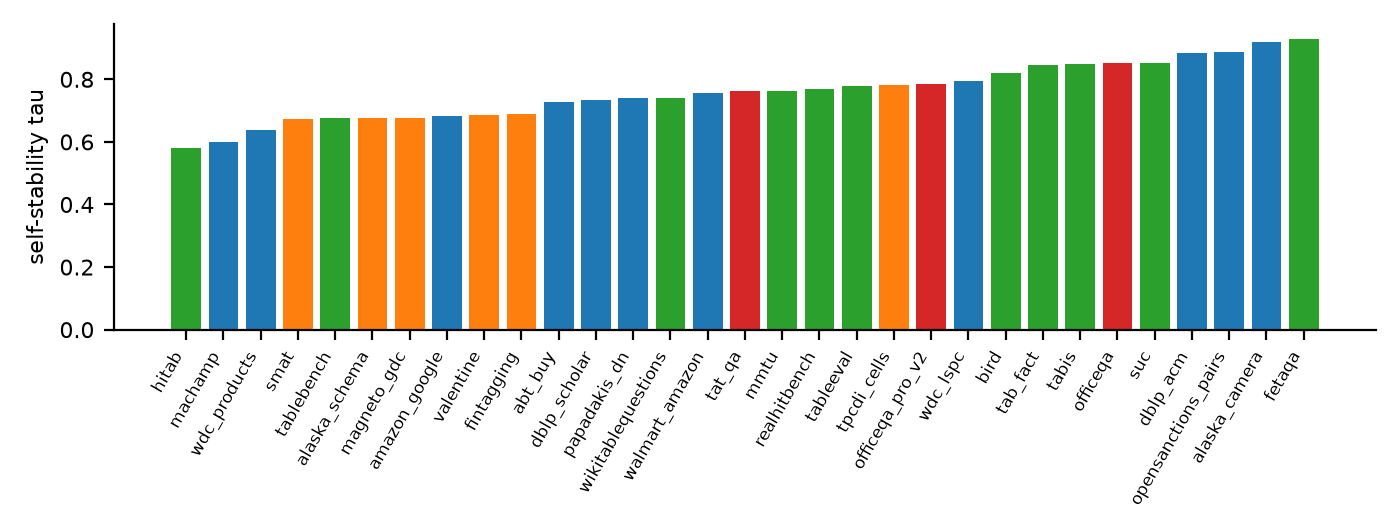
\includegraphics[width=0.9\textwidth]{fig_self_stability.png}\caption{Self-stability of each dataset's model ranking (Kendall $\tau$ between bootstrap halves).}\label{figall:fig_self_stability}\end{figure}
\begin{figure}[htbp]\centering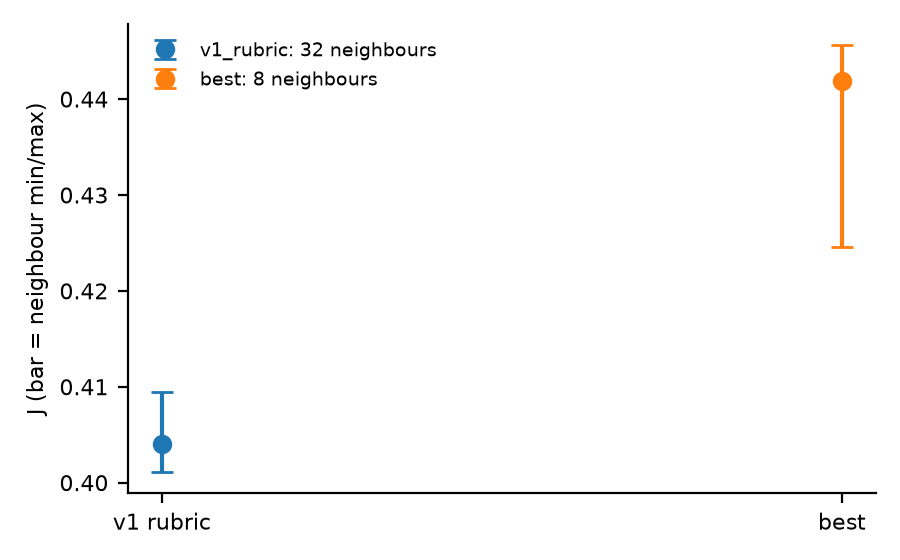
\includegraphics[width=0.9\textwidth]{fig_sensitivity.png}\caption{One-step sensitivity around the v1 rubric and the best candidate.}\label{figall:fig_sensitivity}\end{figure}
\begin{figure}[htbp]\centering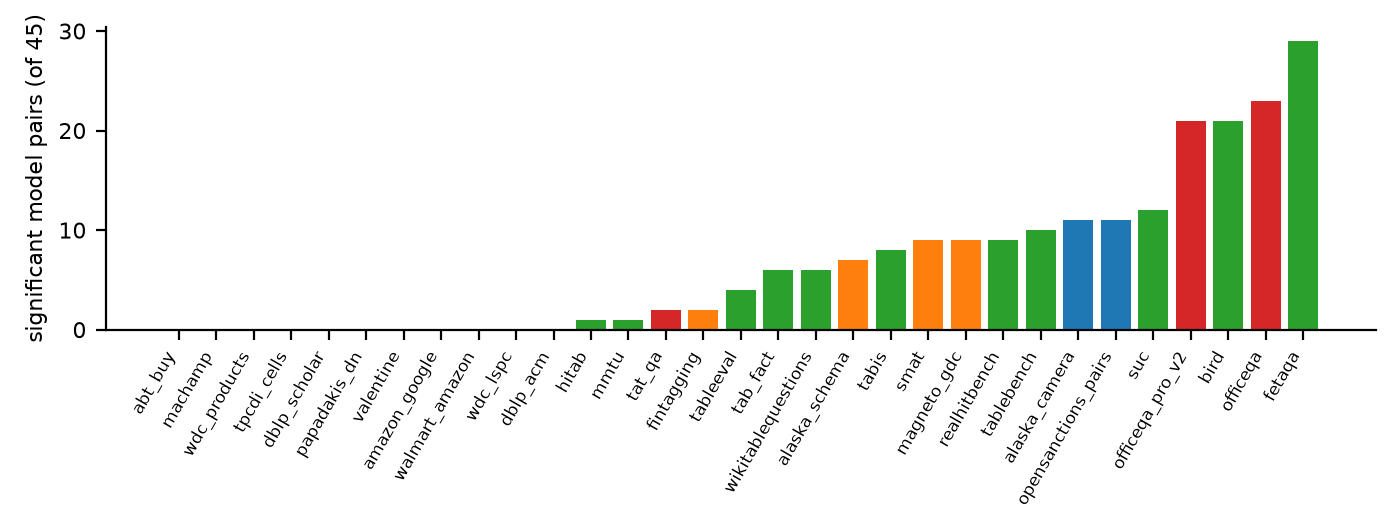
\includegraphics[width=0.9\textwidth]{fig_significant_pairs_per_dataset.png}\caption{How many of the 45 model pairs each dataset separates at the item level under the headline rule (colour = family).}\label{figall:fig_significant_pairs_per_dataset}\end{figure}
\begin{figure}[htbp]\centering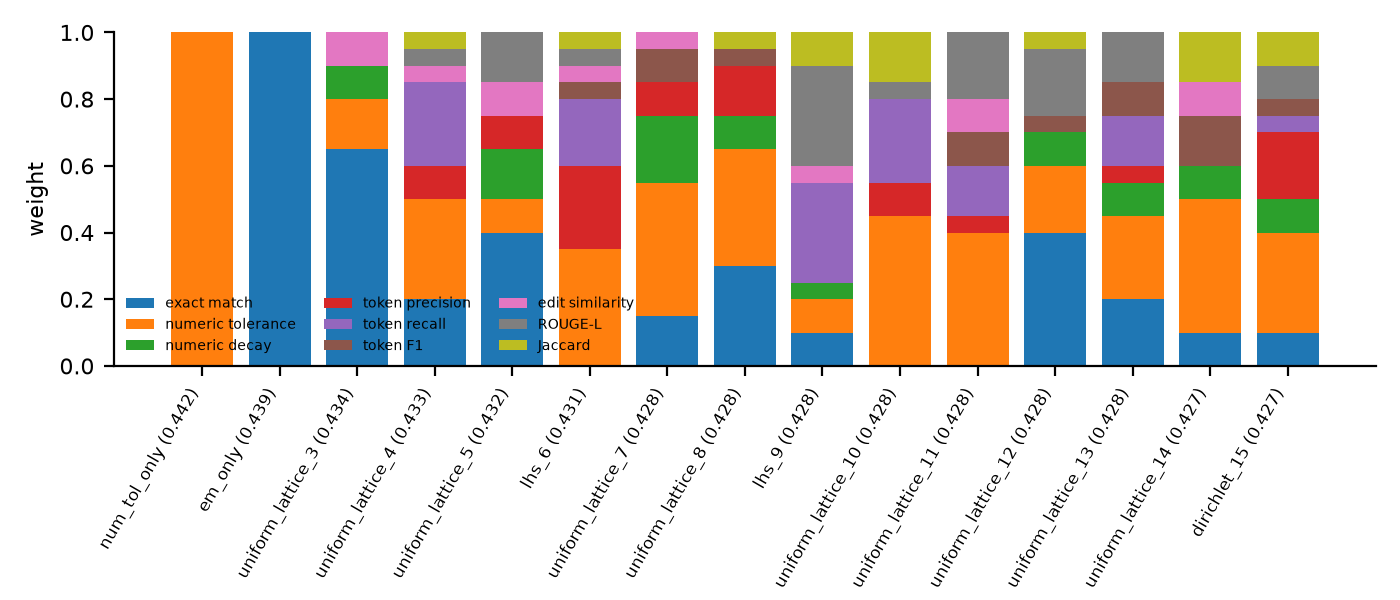
\includegraphics[width=0.9\textwidth]{fig_top_weights.png}\caption{Component weights of the fifteen best candidates.}\label{figall:fig_top_weights}\end{figure}
\clearpage
\section{All tables}
Every saved table, one file each under \texttt{tables/}; include any in the main text with \texttt{\textbackslash input}.
\begin{table}[htbp]
\centering\tiny
\caption{Anchor operators: utility and mean score under three rules.}
\label{tab:anchor_operators}
\setlength{\tabcolsep}{3pt}
\begin{tabular}{p{0.572\linewidth}rrrrrr}
\toprule
op & utility & v1 & bestJ & bestrho & em & n \\
\midrule
no\_\allowbreak{}answer & 0.000 & 0.001 & 0.000 & 0.014 & 0.000 & 3083 \\
wrong\_\allowbreak{}random & 0.000 & 0.097 & 0.042 & 0.101 & 0.041 & 1845 \\
flip & 0.000 & 0.000 & 0.000 & 0.000 & 0.000 & 1238 \\
sign\_\allowbreak{}flip & 0.050 & 0.018 & 0.003 & 0.119 & 0.003 & 632 \\
magnitude & 0.050 & 0.091 & 0.128 & 0.146 & 0.013 & 632 \\
near\_\allowbreak{}miss\_\allowbreak{}large & 0.150 & 0.150 & 0.000 & 0.137 & 0.000 & 632 \\
digit\_\allowbreak{}typo & 0.200 & 0.199 & 0.241 & 0.224 & 0.000 & 632 \\
list\_\allowbreak{}dump & 0.250 & 0.373 & 0.113 & 0.226 & 0.013 & 1845 \\
hedge & 0.300 & 0.493 & 0.405 & 0.392 & 0.192 & 2974 \\
shuffled & 0.400 & 0.652 & 0.009 & 0.418 & 0.009 & 109 \\
near\_\allowbreak{}miss\_\allowbreak{}medium & 0.450 & 0.293 & 0.008 & 0.252 & 0.008 & 632 \\
partial & 0.500 & 0.345 & 0.061 & 0.350 & 0.061 & 1213 \\
superset & 0.600 & 0.467 & 0.045 & 0.335 & 0.045 & 1213 \\
typo & 0.600 & 0.334 & 0.101 & 0.355 & 0.101 & 1104 \\
near\_\allowbreak{}miss\_\allowbreak{}small & 0.750 & 0.405 & 0.101 & 0.366 & 0.097 & 632 \\
paraphrase & 0.950 & 0.965 & 0.964 & 0.958 & 0.930 & 3083 \\
verbose & 1.000 & 1.000 & 0.999 & 1.000 & 0.999 & 3083 \\
identity & 1.000 & 1.000 & 0.999 & 1.000 & 0.999 & 3083 \\
tagged & 1.000 & 1.000 & 0.999 & 1.000 & 0.999 & 3083 \\
unit\_\allowbreak{}variant & 1.000 & 0.898 & 1.000 & 0.891 & 0.837 & 632 \\
\bottomrule
\end{tabular}
\end{table}

\clearpage
\begin{landscape}
\begin{table}[htbp]
\centering\tiny
\caption{Anchor correctness for the labelled candidates.}
\label{tab:anchors_rules}
\setlength{\tabcolsep}{3pt}
\resizebox{\linewidth}{!}{%
\begin{tabular}{lrrrrrrrrrrrrrrr}
\toprule
label & w\_\allowbreak{}em & w\_\allowbreak{}num\_\allowbreak{}tol & w\_\allowbreak{}num\_\allowbreak{}decay & w\_\allowbreak{}tok\_\allowbreak{}prec & w\_\allowbreak{}tok\_\allowbreak{}rec & w\_\allowbreak{}tok\_\allowbreak{}f1 & w\_\allowbreak{}edit\_\allowbreak{}sim & w\_\allowbreak{}rouge\_\allowbreak{}l & w\_\allowbreak{}jaccard & J & rho & rho\_\allowbreak{}ds & auc & wrong\_\allowbreak{}mean & hedge\_\allowbreak{}gap \\
\midrule
num\_\allowbreak{}tol\_\allowbreak{}only & 0.000 & 1.000 & 0.000 & 0.000 & 0.000 & 0.000 & 0.000 & 0.000 & 0.000 & 0.442 & 0.796 & 0.808 & 0.989 & 0.022 & -0.595 \\
em\_\allowbreak{}only & 1.000 & 0.000 & 0.000 & 0.000 & 0.000 & 0.000 & 0.000 & 0.000 & 0.000 & 0.439 & 0.828 & 0.830 & 0.989 & 0.011 & -0.807 \\
uniform & 0.111 & 0.111 & 0.111 & 0.111 & 0.111 & 0.111 & 0.111 & 0.111 & 0.111 & 0.412 & 0.878 & 0.861 & 0.994 & 0.046 & -0.555 \\
f1\_\allowbreak{}only & 0.000 & 0.000 & 0.000 & 0.000 & 0.000 & 1.000 & 0.000 & 0.000 & 0.000 & 0.411 & 0.856 & 0.846 & 0.989 & 0.030 & -0.496 \\
v1\_\allowbreak{}rubric & 0.000 & 0.000 & 0.350 & 0.150 & 0.150 & 0.350 & 0.000 & 0.000 & 0.000 & 0.404 & 0.878 & 0.868 & 0.994 & 0.034 & -0.506 \\
\bottomrule
\end{tabular}
}
\end{table}
\end{landscape}

\clearpage
\begin{landscape}
\begin{table}[htbp]
\centering\tiny
\caption{The five fixed baselines on the candidate set.}
\label{tab:baselines}
\setlength{\tabcolsep}{3pt}
\resizebox{\linewidth}{!}{%
\begin{tabular}{lrrrrrrrrrrrrrrr}
\toprule
rank & label & w\_\allowbreak{}em & w\_\allowbreak{}num\_\allowbreak{}tol & w\_\allowbreak{}num\_\allowbreak{}decay & w\_\allowbreak{}tok\_\allowbreak{}prec & w\_\allowbreak{}tok\_\allowbreak{}rec & w\_\allowbreak{}tok\_\allowbreak{}f1 & w\_\allowbreak{}edit\_\allowbreak{}sim & w\_\allowbreak{}rouge\_\allowbreak{}l & w\_\allowbreak{}jaccard & J & J\_\allowbreak{}kemeny & J\_\allowbreak{}copeland & J\_\allowbreak{}bt & tau\_\allowbreak{}native \\
\midrule
1 & num\_\allowbreak{}tol\_\allowbreak{}only & 0.000 & 1.000 & 0.000 & 0.000 & 0.000 & 0.000 & 0.000 & 0.000 & 0.000 & 0.442 & 0.442 & 0.444 & 0.426 & 0.974 \\
2 & em\_\allowbreak{}only & 1.000 & 0.000 & 0.000 & 0.000 & 0.000 & 0.000 & 0.000 & 0.000 & 0.000 & 0.439 & 0.441 & 0.441 & 0.419 & 0.922 \\
189 & uniform & 0.111 & 0.111 & 0.111 & 0.111 & 0.111 & 0.111 & 0.111 & 0.111 & 0.111 & 0.412 & 0.418 & 0.427 & 0.395 & 0.916 \\
217 & f1\_\allowbreak{}only & 0.000 & 0.000 & 0.000 & 0.000 & 0.000 & 1.000 & 0.000 & 0.000 & 0.000 & 0.411 & 0.418 & 0.422 & 0.375 & 0.893 \\
295 & v1\_\allowbreak{}rubric & 0.000 & 0.000 & 0.350 & 0.150 & 0.150 & 0.350 & 0.000 & 0.000 & 0.000 & 0.404 & 0.408 & 0.409 & 0.390 & 0.912 \\
\bottomrule
\end{tabular}
}
\end{table}
\end{landscape}

\clearpage
\begin{landscape}
\begin{table}[htbp]
\centering\tiny
\caption{Sampled designs: summary over 20 seeds.}
\label{tab:designs_summary}
\setlength{\tabcolsep}{3pt}
\resizebox{\linewidth}{!}{%
\begin{tabular}{lrrrrrrrrrr}
\toprule
design & best\_\allowbreak{}J\_\allowbreak{}mean & best\_\allowbreak{}J\_\allowbreak{}sd & best\_\allowbreak{}J\_\allowbreak{}max & mean\_\allowbreak{}J & regret\_\allowbreak{}mean & regret\_\allowbreak{}max & min\_\allowbreak{}pairwise\_\allowbreak{}L1 & mean\_\allowbreak{}nearest\_\allowbreak{}L1 & discrepancy & zero\_\allowbreak{}share \\
\midrule
dirichlet\_\allowbreak{}lattice & 0.4320 & 0.0030 & 0.4391 & 0.4153 & 0.0100 & 0.0138 & 0.1950 & 0.4027 & 2.6738 & 0.8820 \\
lhs\_\allowbreak{}simplex & 0.4313 & 0.0022 & 0.4373 & 0.4151 & 0.0107 & 0.0141 & 0.2150 & 0.4096 & 2.6718 & 0.8780 \\
uniform\_\allowbreak{}lattice & 0.4343 & 0.0033 & 0.4420 & 0.4155 & 0.0077 & 0.0129 & 0.2350 & 0.4650 & 2.5904 & 0.9705 \\
\bottomrule
\end{tabular}
}
\end{table}
\end{landscape}

\clearpage
\begin{landscape}
\tiny
\setlength{\tabcolsep}{3pt}
\begin{longtable}{p{0.147\linewidth}p{0.073\linewidth}p{0.073\linewidth}p{0.073\linewidth}p{0.073\linewidth}p{0.073\linewidth}p{0.073\linewidth}p{0.073\linewidth}p{0.073\linewidth}p{0.073\linewidth}p{0.073\linewidth}}
\caption{Dataset diagnostics under the headline rule.}\label{tab:diagnostics}\\
\toprule
dataset & family & mean\_\allowbreak{}score & spread\_\allowbreak{}across\_\allowbreak{}models & floor & ceiling & share\_\allowbreak{}constant\_\allowbreak{}bootstrap\_\allowbreak{}rankings & ranking\_\allowbreak{}self\_\allowbreak{}stability\_\allowbreak{}tau & tau\_\allowbreak{}to\_\allowbreak{}others\_\allowbreak{}mean & n\_\allowbreak{}items & exclude\_\allowbreak{}from\_\allowbreak{}objective \\
\midrule
abt\_\allowbreak{}buy & EM & 0.970 & 0.060 & no & no & 0.000 & 0.726 & 0.356 & 100 & no \\
alaska\_\allowbreak{}camera & EM & 0.958 & 0.180 & no & no & 0.000 & 0.919 & -0.218 & 100 & no \\
alaska\_\allowbreak{}schema & SM & 0.928 & 0.118 & no & no & 0.000 & 0.675 & -0.044 & 93 & no \\
amazon\_\allowbreak{}google & EM & 0.936 & 0.100 & no & no & 0.000 & 0.684 & -0.012 & 100 & no \\
bird & TQA & 0.187 & 0.209 & no & no & 0.000 & 0.820 & 0.313 & 100 & no \\
dblp\_\allowbreak{}acm & EM & 0.986 & 0.090 & no & no & 0.000 & 0.884 & 0.350 & 100 & no \\
dblp\_\allowbreak{}scholar & EM & 0.949 & 0.060 & no & no & 0.000 & 0.733 & -0.019 & 100 & no \\
fetaqa & TQA & 0.382 & 0.192 & no & no & 0.000 & 0.930 & 0.271 & 100 & no \\
fintagging & SM & 0.880 & 0.069 & no & no & 0.000 & 0.689 & 0.256 & 100 & no \\
hitab & TQA & 0.770 & 0.068 & no & no & 0.000 & 0.581 & -0.181 & 100 & no \\
machamp & EM & 0.887 & 0.070 & no & no & 0.000 & 0.600 & 0.377 & 100 & no \\
magneto\_\allowbreak{}gdc & SM & 0.934 & 0.218 & no & no & 0.000 & 0.677 & 0.252 & 100 & no \\
mmtu & TQA & 0.867 & 0.110 & no & no & 0.000 & 0.763 & 0.298 & 100 & no \\
officeqa & FIN & 0.129 & 0.119 & no & no & 0.000 & 0.853 & 0.276 & 100 & no \\
officeqa\_\allowbreak{}pro\_\allowbreak{}v2 & FIN & 0.139 & 0.215 & no & no & 0.000 & 0.785 & 0.311 & 90 & no \\
opensanctions\_\allowbreak{}pairs & EM & 0.821 & 0.210 & no & no & 0.000 & 0.888 & 0.030 & 100 & no \\
papadakis\_\allowbreak{}dn & EM & 0.941 & 0.030 & no & no & 0.002 & 0.739 & 0.067 & 100 & no \\
realhitbench & TQA & 0.673 & 0.143 & no & no & 0.000 & 0.769 & 0.344 & 100 & no \\
smat & SM & 0.918 & 0.150 & no & no & 0.000 & 0.674 & 0.200 & 100 & no \\
suc & TQA & 0.914 & 0.246 & no & no & 0.000 & 0.853 & 0.293 & 100 & no \\
tab\_\allowbreak{}fact & TQA & 0.798 & 0.200 & no & no & 0.000 & 0.845 & 0.007 & 100 & no \\
tabis & TQA & 0.915 & 0.210 & no & no & 0.000 & 0.849 & 0.224 & 100 & no \\
tablebench & TQA & 0.818 & 0.218 & no & no & 0.000 & 0.675 & 0.276 & 100 & no \\
tableeval & TQA & 0.749 & 0.166 & no & no & 0.000 & 0.778 & 0.195 & 100 & no \\
tat\_\allowbreak{}qa & FIN & 0.803 & 0.109 & no & no & 0.000 & 0.762 & 0.262 & 100 & no \\
tpcdi\_\allowbreak{}cells & SM & 0.456 & 0.020 & no & no & 0.000 & 0.782 & 0.298 & 100 & no \\
valentine & SM & 0.984 & 0.030 & no & yes & 0.000 & 0.685 & 0.229 & 100 & yes \\
walmart\_\allowbreak{}amazon & EM & 0.958 & 0.060 & no & no & 0.000 & 0.755 & 0.360 & 100 & no \\
wdc\_\allowbreak{}lspc & EM & 0.982 & 0.040 & no & yes & 0.004 & 0.796 & 0.246 & 100 & yes \\
wdc\_\allowbreak{}products & EM & 0.978 & 0.020 & no & yes & 0.006 & 0.637 & 0.178 & 100 & yes \\
wikitablequestions & TQA & 0.846 & 0.132 & no & no & 0.000 & 0.739 & 0.350 & 100 & no \\
\bottomrule
\end{longtable}
\normalsize
\end{landscape}

\clearpage
\begin{table}[htbp]
\centering\scriptsize
\caption{Mean v1-rubric score per model within each family.}
\label{tab:family_scores}
\setlength{\tabcolsep}{3pt}
\begin{tabular}{p{0.278\linewidth}p{0.261\linewidth}rp{0.261\linewidth}r}
\toprule
model & entity matching & finance & schema matching & table QA \\
\midrule
Gemini 3.8 Flash & 0.945 & 0.414 & 0.854 & 0.765 \\
Claude Opus 5 & 0.947 & 0.439 & 0.869 & 0.745 \\
GPT-5.5 & 0.950 & 0.388 & 0.864 & 0.751 \\
Claude Sonnet 5 & 0.942 & 0.391 & 0.862 & 0.724 \\
Grok 4 & 0.948 & 0.354 & 0.851 & 0.738 \\
GPT-5.4-mini & 0.947 & 0.347 & 0.859 & 0.716 \\
DeepSeek-chat & 0.941 & 0.342 & 0.852 & 0.711 \\
DeepSeek-R1 & 0.953 & 0.318 & 0.853 & 0.717 \\
gpt-oss-120b & 0.915 & 0.323 & 0.848 & 0.698 \\
Llama 3.3 70B & 0.936 & 0.328 & 0.777 & 0.633 \\
\bottomrule
\end{tabular}
\end{table}

\clearpage
\begin{landscape}
\tiny
\setlength{\tabcolsep}{3pt}
\begin{longtable}{p{0.098\linewidth}p{0.049\linewidth}p{0.049\linewidth}p{0.049\linewidth}p{0.049\linewidth}p{0.049\linewidth}p{0.049\linewidth}p{0.049\linewidth}p{0.049\linewidth}p{0.049\linewidth}p{0.049\linewidth}p{0.049\linewidth}p{0.049\linewidth}p{0.049\linewidth}p{0.049\linewidth}p{0.049\linewidth}}
\caption{The 25 best candidates with the objective under the other pooling rules.}\label{tab:grid_top25}\\
\toprule
rank & label & w\_\allowbreak{}em & w\_\allowbreak{}num\_\allowbreak{}tol & w\_\allowbreak{}num\_\allowbreak{}decay & w\_\allowbreak{}tok\_\allowbreak{}prec & w\_\allowbreak{}tok\_\allowbreak{}rec & w\_\allowbreak{}tok\_\allowbreak{}f1 & w\_\allowbreak{}edit\_\allowbreak{}sim & w\_\allowbreak{}rouge\_\allowbreak{}l & w\_\allowbreak{}jaccard & J & J\_\allowbreak{}kemeny & J\_\allowbreak{}copeland & J\_\allowbreak{}bt & tau\_\allowbreak{}native \\
\midrule
1 & num\_\allowbreak{}tol\_\allowbreak{}only & 0.000 & 1.000 & 0.000 & 0.000 & 0.000 & 0.000 & 0.000 & 0.000 & 0.000 & 0.442 & 0.442 & 0.444 & 0.426 & 0.974 \\
2 & em\_\allowbreak{}only & 1.000 & 0.000 & 0.000 & 0.000 & 0.000 & 0.000 & 0.000 & 0.000 & 0.000 & 0.439 & 0.441 & 0.441 & 0.419 & 0.922 \\
3 & uniform\_\allowbreak{}lattice\_\allowbreak{}3 & 0.650 & 0.150 & 0.100 & 0.000 & 0.000 & 0.000 & 0.100 & 0.000 & 0.000 & 0.434 & 0.434 & 0.434 & 0.398 & 0.907 \\
4 & uniform\_\allowbreak{}lattice\_\allowbreak{}4 & 0.200 & 0.300 & 0.000 & 0.100 & 0.250 & 0.000 & 0.050 & 0.050 & 0.050 & 0.433 & 0.433 & 0.433 & 0.387 & 0.933 \\
5 & uniform\_\allowbreak{}lattice\_\allowbreak{}5 & 0.400 & 0.100 & 0.150 & 0.100 & 0.000 & 0.000 & 0.100 & 0.150 & 0.000 & 0.432 & 0.431 & 0.440 & 0.408 & 0.916 \\
6 & lhs\_\allowbreak{}6 & 0.000 & 0.350 & 0.000 & 0.250 & 0.200 & 0.050 & 0.050 & 0.050 & 0.050 & 0.431 & 0.435 & 0.435 & 0.401 & 0.927 \\
7 & uniform\_\allowbreak{}lattice\_\allowbreak{}7 & 0.150 & 0.400 & 0.200 & 0.100 & 0.000 & 0.100 & 0.050 & 0.000 & 0.000 & 0.428 & 0.429 & 0.431 & 0.405 & 0.932 \\
8 & uniform\_\allowbreak{}lattice\_\allowbreak{}8 & 0.300 & 0.350 & 0.100 & 0.150 & 0.000 & 0.050 & 0.000 & 0.000 & 0.050 & 0.428 & 0.432 & 0.431 & 0.399 & 0.930 \\
9 & lhs\_\allowbreak{}9 & 0.100 & 0.100 & 0.050 & 0.000 & 0.300 & 0.000 & 0.050 & 0.300 & 0.100 & 0.428 & 0.431 & 0.431 & 0.398 & 0.907 \\
10 & uniform\_\allowbreak{}lattice\_\allowbreak{}10 & 0.000 & 0.450 & 0.000 & 0.100 & 0.250 & 0.000 & 0.000 & 0.050 & 0.150 & 0.428 & 0.428 & 0.428 & 0.404 & 0.932 \\
11 & uniform\_\allowbreak{}lattice\_\allowbreak{}11 & 0.000 & 0.400 & 0.000 & 0.050 & 0.150 & 0.100 & 0.100 & 0.200 & 0.000 & 0.428 & 0.432 & 0.432 & 0.392 & 0.933 \\
12 & uniform\_\allowbreak{}lattice\_\allowbreak{}12 & 0.400 & 0.200 & 0.100 & 0.000 & 0.000 & 0.050 & 0.000 & 0.200 & 0.050 & 0.428 & 0.433 & 0.442 & 0.410 & 0.930 \\
13 & uniform\_\allowbreak{}lattice\_\allowbreak{}13 & 0.200 & 0.250 & 0.100 & 0.050 & 0.150 & 0.100 & 0.000 & 0.150 & 0.000 & 0.428 & 0.429 & 0.427 & 0.401 & 0.935 \\
14 & uniform\_\allowbreak{}lattice\_\allowbreak{}14 & 0.100 & 0.400 & 0.100 & 0.000 & 0.000 & 0.150 & 0.100 & 0.000 & 0.150 & 0.427 & 0.428 & 0.434 & 0.409 & 0.938 \\
15 & dirichlet\_\allowbreak{}15 & 0.100 & 0.300 & 0.100 & 0.200 & 0.050 & 0.050 & 0.000 & 0.100 & 0.100 & 0.427 & 0.434 & 0.434 & 0.405 & 0.932 \\
16 & lhs\_\allowbreak{}16 & 0.100 & 0.450 & 0.100 & 0.050 & 0.050 & 0.000 & 0.000 & 0.200 & 0.050 & 0.427 & 0.433 & 0.432 & 0.408 & 0.944 \\
17 & lhs\_\allowbreak{}17 & 0.050 & 0.300 & 0.100 & 0.100 & 0.100 & 0.050 & 0.050 & 0.150 & 0.100 & 0.426 & 0.432 & 0.432 & 0.403 & 0.930 \\
18 & uniform\_\allowbreak{}lattice\_\allowbreak{}18 & 0.100 & 0.400 & 0.100 & 0.150 & 0.100 & 0.050 & 0.100 & 0.000 & 0.000 & 0.426 & 0.426 & 0.427 & 0.405 & 0.935 \\
19 & dirichlet\_\allowbreak{}19 & 0.050 & 0.300 & 0.050 & 0.000 & 0.100 & 0.100 & 0.050 & 0.050 & 0.300 & 0.425 & 0.428 & 0.428 & 0.393 & 0.929 \\
20 & lhs\_\allowbreak{}20 & 0.250 & 0.150 & 0.350 & 0.000 & 0.000 & 0.150 & 0.000 & 0.050 & 0.050 & 0.425 & 0.427 & 0.427 & 0.410 & 0.926 \\
21 & dirichlet\_\allowbreak{}21 & 0.200 & 0.250 & 0.000 & 0.100 & 0.100 & 0.000 & 0.050 & 0.100 & 0.200 & 0.425 & 0.432 & 0.437 & 0.391 & 0.929 \\
22 & lhs\_\allowbreak{}22 & 0.100 & 0.100 & 0.000 & 0.100 & 0.400 & 0.050 & 0.050 & 0.050 & 0.150 & 0.425 & 0.426 & 0.426 & 0.384 & 0.912 \\
23 & dirichlet\_\allowbreak{}23 & 0.350 & 0.050 & 0.050 & 0.000 & 0.150 & 0.000 & 0.000 & 0.400 & 0.000 & 0.425 & 0.430 & 0.437 & 0.401 & 0.920 \\
24 & lhs\_\allowbreak{}24 & 0.150 & 0.050 & 0.050 & 0.050 & 0.500 & 0.000 & 0.000 & 0.050 & 0.150 & 0.425 & 0.425 & 0.425 & 0.404 & 0.909 \\
25 & lhs\_\allowbreak{}25 & 0.050 & 0.100 & 0.050 & 0.000 & 0.450 & 0.150 & 0.000 & 0.100 & 0.100 & 0.425 & 0.425 & 0.429 & 0.404 & 0.908 \\
\bottomrule
\end{longtable}
\normalsize
\end{landscape}

\clearpage
\begin{landscape}
\begin{table}[htbp]
\centering\tiny
\caption{Full leaderboard under rule best-rho; weights: em 0.20, num\_\allowbreak{}decay 0.25, tok\_\allowbreak{}prec 0.25, tok\_\allowbreak{}rec 0.05, tok\_\allowbreak{}f1 0.05, edit\_\allowbreak{}sim 0.15, rouge\_\allowbreak{}l 0.05.}
\label{tab:leaderboard_best_anchor}
\setlength{\tabcolsep}{3pt}
\resizebox{\linewidth}{!}{%
\begin{tabular}{lrrrrrrrrrrrrrrrr}
\toprule
model & bt\_\allowbreak{}strength & bt\_\allowbreak{}se\_\allowbreak{}vs\_\allowbreak{}ref & rank\_\allowbreak{}bt & bt\_\allowbreak{}rank\_\allowbreak{}lo95 & bt\_\allowbreak{}rank\_\allowbreak{}hi95 & p\_\allowbreak{}first\_\allowbreak{}bt & rank\_\allowbreak{}borda & borda\_\allowbreak{}rank\_\allowbreak{}lo95 & borda\_\allowbreak{}rank\_\allowbreak{}hi95 & p\_\allowbreak{}first\_\allowbreak{}borda & rank\_\allowbreak{}kemeny & rank\_\allowbreak{}copeland & rank\_\allowbreak{}mean\_\allowbreak{}z & rank\_\allowbreak{}rrf & rank\_\allowbreak{}family\_\allowbreak{}balanced\_\allowbreak{}z & mean\_\allowbreak{}score \\
\midrule
Gemini 3.8 Flash & 0.125 & 0.016 & 1.000 & 1.000 & 2.000 & 0.968 & 3.000 & 2.000 & 3.012 & 0.017 & 3.000 & 3.000 & 3.000 & 3.000 & 2.000 & 0.806 \\
Claude Opus 5 & 0.103 & 0.000 & 2.000 & 1.000 & 2.000 & 0.032 & 2.000 & 1.000 & 3.000 & 0.541 & 1.000 & 1.000 & 1.000 & 2.000 & 1.000 & 0.806 \\
GPT-5.5 & 0.058 & 0.016 & 3.000 & 3.000 & 3.000 & 0.000 & 1.000 & 1.000 & 3.000 & 0.433 & 2.000 & 2.000 & 2.000 & 1.000 & 3.000 & 0.803 \\
Claude Sonnet 5 & 0.031 & 0.016 & 4.000 & 4.000 & 5.000 & 0.000 & 4.000 & 4.000 & 6.025 & 0.000 & 4.000 & 4.000 & 4.000 & 4.000 & 4.000 & 0.790 \\
Grok 4 & 0.018 & 0.016 & 5.000 & 4.000 & 6.000 & 0.000 & 5.000 & 4.000 & 6.000 & 0.000 & 5.000 & 5.000 & 5.000 & 5.000 & 5.000 & 0.792 \\
GPT-5.4-mini & 0.003 & 0.016 & 6.000 & 5.000 & 7.000 & 0.000 & 7.000 & 5.000 & 8.000 & 0.000 & 6.000 & 7.000 & 6.000 & 7.000 & 6.000 & 0.787 \\
DeepSeek-chat & -0.024 & 0.016 & 7.000 & 6.000 & 7.000 & 0.000 & 8.000 & 5.000 & 8.000 & 0.000 & 7.000 & 7.000 & 8.000 & 8.000 & 7.000 & 0.778 \\
DeepSeek-R1 & -0.055 & 0.016 & 8.000 & 8.000 & 8.000 & 0.000 & 6.000 & 4.500 & 8.000 & 0.000 & 8.000 & 7.000 & 7.000 & 6.000 & 8.000 & 0.781 \\
gpt-oss-120b & -0.117 & 0.016 & 9.000 & 9.000 & 10.000 & 0.000 & 9.000 & 9.000 & 10.000 & 0.000 & 9.000 & 9.000 & 9.000 & 9.000 & 9.000 & 0.762 \\
Llama 3.3 70B & -0.142 & 0.016 & 10.000 & 9.000 & 10.000 & 0.000 & 10.000 & 9.000 & 10.000 & 0.000 & 10.000 & 10.000 & 10.000 & 10.000 & 10.000 & 0.733 \\
\bottomrule
\end{tabular}
}
\end{table}
\end{landscape}

\clearpage
\begin{landscape}
\begin{table}[htbp]
\centering\tiny
\caption{Full leaderboard under rule exact match; weights: em 1.00.}
\label{tab:leaderboard_em_only}
\setlength{\tabcolsep}{3pt}
\resizebox{\linewidth}{!}{%
\begin{tabular}{lrrrrrrrrrrrrrrrr}
\toprule
model & bt\_\allowbreak{}strength & bt\_\allowbreak{}se\_\allowbreak{}vs\_\allowbreak{}ref & rank\_\allowbreak{}bt & bt\_\allowbreak{}rank\_\allowbreak{}lo95 & bt\_\allowbreak{}rank\_\allowbreak{}hi95 & p\_\allowbreak{}first\_\allowbreak{}bt & rank\_\allowbreak{}borda & borda\_\allowbreak{}rank\_\allowbreak{}lo95 & borda\_\allowbreak{}rank\_\allowbreak{}hi95 & p\_\allowbreak{}first\_\allowbreak{}borda & rank\_\allowbreak{}kemeny & rank\_\allowbreak{}copeland & rank\_\allowbreak{}mean\_\allowbreak{}z & rank\_\allowbreak{}rrf & rank\_\allowbreak{}family\_\allowbreak{}balanced\_\allowbreak{}z & mean\_\allowbreak{}score \\
\midrule
Claude Opus 5 & 0.047 & 0.000 & 1.000 & 1.000 & 3.000 & 0.764 & 1.000 & 1.000 & 2.000 & 0.812 & 1.000 & 1.000 & 1.000 & 1.000 & 1.000 & 0.768 \\
GPT-5.5 & 0.039 & 0.016 & 2.000 & 1.000 & 3.000 & 0.152 & 2.000 & 1.000 & 3.000 & 0.177 & 2.000 & 2.000 & 2.000 & 2.000 & 2.000 & 0.764 \\
Gemini 3.8 Flash & 0.037 & 0.016 & 3.000 & 1.000 & 3.000 & 0.084 & 3.000 & 2.000 & 5.000 & 0.004 & 3.000 & 3.000 & 3.000 & 3.000 & 3.000 & 0.763 \\
Grok 4 & 0.020 & 0.016 & 4.000 & 4.000 & 6.000 & 0.000 & 5.000 & 3.000 & 6.012 & 0.000 & 5.000 & 5.000 & 5.000 & 5.000 & 5.000 & 0.754 \\
Claude Sonnet 5 & 0.013 & 0.016 & 5.000 & 4.000 & 7.000 & 0.000 & 4.000 & 3.000 & 6.000 & 0.000 & 4.000 & 4.000 & 4.000 & 4.000 & 4.000 & 0.751 \\
GPT-5.4-mini & 0.010 & 0.016 & 6.000 & 4.000 & 7.000 & 0.000 & 8.000 & 6.000 & 8.000 & 0.000 & 7.000 & 7.000 & 7.000 & 8.000 & 8.000 & 0.749 \\
DeepSeek-R1 & 0.008 & 0.016 & 7.000 & 5.000 & 7.000 & 0.000 & 6.000 & 4.000 & 8.000 & 0.000 & 6.000 & 6.000 & 6.000 & 6.000 & 6.000 & 0.748 \\
DeepSeek-chat & -0.014 & 0.016 & 8.000 & 8.000 & 9.000 & 0.000 & 7.000 & 6.000 & 8.000 & 0.000 & 8.000 & 8.000 & 8.000 & 7.000 & 7.000 & 0.737 \\
gpt-oss-120b & -0.033 & 0.016 & 9.000 & 8.000 & 9.000 & 0.000 & 9.000 & 9.000 & 9.000 & 0.000 & 9.000 & 9.000 & 9.000 & 9.000 & 9.000 & 0.728 \\
Llama 3.3 70B & -0.128 & 0.016 & 10.000 & 10.000 & 10.000 & 0.000 & 10.000 & 10.000 & 10.000 & 0.000 & 10.000 & 10.000 & 10.000 & 10.000 & 10.000 & 0.680 \\
\bottomrule
\end{tabular}
}
\end{table}
\end{landscape}

\clearpage
\begin{table}[htbp]
\centering\tiny
\caption{Leaderboard under the headline rule (v1 rubric).}
\label{tab:leaderboard_headline}
\setlength{\tabcolsep}{3pt}
\begin{tabular}{lp{0.256\linewidth}p{0.176\linewidth}rrrp{0.176\linewidth}r}
\toprule
rank & model & BT strength & SE & Borda rank & Borda 95\% & P(first) BT & mean score \\
\midrule
1 & Gemini 3.8 Flash & 0.121 & 0.016 & 3 & [1, 3] & 0.990 & 0.812 \\
2 & Claude Opus 5 & 0.095 & 0.000 & 2 & [1, 3] & 0.010 & 0.811 \\
3 & GPT-5.5 & 0.052 & 0.016 & 1 & [1, 3] & 0.000 & 0.808 \\
4 & Claude Sonnet 5 & 0.029 & 0.016 & 4 & [4, 6] & 0.000 & 0.795 \\
5 & Grok 4 & 0.027 & 0.016 & 5 & [4, 6] & 0.000 & 0.797 \\
6 & GPT-5.4-mini & -0.010 & 0.016 & 8 & [5, 8] & 0.000 & 0.790 \\
7 & DeepSeek-chat & -0.018 & 0.016 & 7 & [5, 8] & 0.000 & 0.784 \\
8 & DeepSeek-R1 & -0.025 & 0.016 & 6 & [5, 8] & 0.000 & 0.788 \\
9 & gpt-oss-120b & -0.100 & 0.016 & 9 & [9, 10] & 0.000 & 0.767 \\
10 & Llama 3.3 70B & -0.170 & 0.016 & 10 & [9, 10] & 0.000 & 0.738 \\
\bottomrule
\end{tabular}
\end{table}

\clearpage
\begin{landscape}
\begin{table}[htbp]
\centering\tiny
\caption{Full leaderboard under rule knee; weights: em 0.40, num\_\allowbreak{}tol 0.10, num\_\allowbreak{}decay 0.15, tok\_\allowbreak{}prec 0.10, edit\_\allowbreak{}sim 0.10, rouge\_\allowbreak{}l 0.15.}
\label{tab:leaderboard_pareto_knee}
\setlength{\tabcolsep}{3pt}
\resizebox{\linewidth}{!}{%
\begin{tabular}{lrrrrrrrrrrrrrrrr}
\toprule
model & bt\_\allowbreak{}strength & bt\_\allowbreak{}se\_\allowbreak{}vs\_\allowbreak{}ref & rank\_\allowbreak{}bt & bt\_\allowbreak{}rank\_\allowbreak{}lo95 & bt\_\allowbreak{}rank\_\allowbreak{}hi95 & p\_\allowbreak{}first\_\allowbreak{}bt & rank\_\allowbreak{}borda & borda\_\allowbreak{}rank\_\allowbreak{}lo95 & borda\_\allowbreak{}rank\_\allowbreak{}hi95 & p\_\allowbreak{}first\_\allowbreak{}borda & rank\_\allowbreak{}kemeny & rank\_\allowbreak{}copeland & rank\_\allowbreak{}mean\_\allowbreak{}z & rank\_\allowbreak{}rrf & rank\_\allowbreak{}family\_\allowbreak{}balanced\_\allowbreak{}z & mean\_\allowbreak{}score \\
\midrule
Gemini 3.8 Flash & 0.125 & 0.016 & 1.000 & 1.000 & 2.000 & 0.920 & 3.000 & 2.000 & 4.000 & 0.014 & 3.000 & 3.000 & 3.000 & 3.000 & 3.000 & 0.790 \\
Claude Opus 5 & 0.109 & 0.000 & 2.000 & 1.000 & 2.000 & 0.080 & 1.500 & 1.000 & 3.000 & 0.597 & 1.000 & 1.000 & 1.000 & 1.000 & 1.000 & 0.792 \\
GPT-5.5 & 0.059 & 0.016 & 3.000 & 3.000 & 3.000 & 0.000 & 1.500 & 1.000 & 3.000 & 0.381 & 2.000 & 2.000 & 2.000 & 2.000 & 2.000 & 0.788 \\
Claude Sonnet 5 & 0.031 & 0.016 & 4.000 & 4.000 & 5.000 & 0.000 & 4.000 & 4.000 & 6.500 & 0.000 & 4.000 & 4.000 & 4.000 & 4.000 & 4.000 & 0.776 \\
Grok 4 & 0.019 & 0.016 & 5.000 & 4.000 & 6.000 & 0.000 & 5.000 & 4.000 & 6.000 & 0.000 & 5.000 & 5.000 & 5.000 & 5.000 & 5.000 & 0.778 \\
GPT-5.4-mini & -0.001 & 0.016 & 6.000 & 5.000 & 7.000 & 0.000 & 7.000 & 5.000 & 8.000 & 0.000 & 6.000 & 7.000 & 7.000 & 7.000 & 6.000 & 0.773 \\
DeepSeek-chat & -0.022 & 0.016 & 7.000 & 6.000 & 7.000 & 0.000 & 8.000 & 5.000 & 8.000 & 0.000 & 7.000 & 7.000 & 8.000 & 8.000 & 8.000 & 0.763 \\
DeepSeek-R1 & -0.062 & 0.016 & 8.000 & 8.000 & 8.000 & 0.000 & 6.000 & 4.975 & 8.000 & 0.000 & 8.000 & 7.000 & 6.000 & 6.000 & 7.000 & 0.768 \\
gpt-oss-120b & -0.111 & 0.016 & 9.000 & 9.000 & 9.000 & 0.000 & 9.000 & 9.000 & 10.000 & 0.000 & 9.000 & 9.000 & 9.000 & 9.000 & 9.000 & 0.750 \\
Llama 3.3 70B & -0.147 & 0.016 & 10.000 & 10.000 & 10.000 & 0.000 & 10.000 & 9.000 & 10.000 & 0.000 & 10.000 & 10.000 & 10.000 & 10.000 & 10.000 & 0.713 \\
\bottomrule
\end{tabular}
}
\end{table}
\end{landscape}

\clearpage
\begin{landscape}
\begin{table}[htbp]
\centering\tiny
\caption{Full leaderboard under rule top1; weights: num\_\allowbreak{}tol 1.00.}
\label{tab:leaderboard_top1}
\setlength{\tabcolsep}{3pt}
\resizebox{\linewidth}{!}{%
\begin{tabular}{lrrrrrrrrrrrrrrrr}
\toprule
model & bt\_\allowbreak{}strength & bt\_\allowbreak{}se\_\allowbreak{}vs\_\allowbreak{}ref & rank\_\allowbreak{}bt & bt\_\allowbreak{}rank\_\allowbreak{}lo95 & bt\_\allowbreak{}rank\_\allowbreak{}hi95 & p\_\allowbreak{}first\_\allowbreak{}bt & rank\_\allowbreak{}borda & borda\_\allowbreak{}rank\_\allowbreak{}lo95 & borda\_\allowbreak{}rank\_\allowbreak{}hi95 & p\_\allowbreak{}first\_\allowbreak{}borda & rank\_\allowbreak{}kemeny & rank\_\allowbreak{}copeland & rank\_\allowbreak{}mean\_\allowbreak{}z & rank\_\allowbreak{}rrf & rank\_\allowbreak{}family\_\allowbreak{}balanced\_\allowbreak{}z & mean\_\allowbreak{}score \\
\midrule
Claude Opus 5 & 0.046 & 0.000 & 1.000 & 1.000 & 3.000 & 0.538 & 1.000 & 1.000 & 2.000 & 0.613 & 1.000 & 1.000 & 1.000 & 1.000 & 1.000 & 0.778 \\
GPT-5.5 & 0.043 & 0.016 & 2.000 & 1.000 & 3.000 & 0.296 & 2.000 & 1.000 & 3.000 & 0.369 & 2.000 & 2.000 & 2.000 & 2.000 & 2.000 & 0.776 \\
Gemini 3.8 Flash & 0.041 & 0.016 & 3.000 & 1.000 & 3.000 & 0.165 & 3.000 & 2.000 & 4.012 & 0.004 & 3.000 & 3.000 & 3.000 & 3.000 & 3.000 & 0.775 \\
Grok 4 & 0.019 & 0.016 & 4.000 & 4.000 & 6.000 & 0.000 & 5.000 & 3.000 & 6.000 & 0.000 & 5.000 & 4.500 & 5.000 & 5.000 & 5.000 & 0.764 \\
Claude Sonnet 5 & 0.014 & 0.016 & 5.000 & 4.000 & 7.000 & 0.000 & 4.000 & 3.000 & 6.000 & 0.000 & 4.000 & 4.500 & 4.000 & 4.000 & 4.000 & 0.762 \\
GPT-5.4-mini & 0.009 & 0.016 & 6.000 & 4.000 & 7.000 & 0.000 & 7.000 & 6.000 & 8.000 & 0.000 & 7.000 & 7.000 & 7.000 & 7.000 & 7.000 & 0.759 \\
DeepSeek-R1 & 0.006 & 0.016 & 7.000 & 5.000 & 7.000 & 0.000 & 6.000 & 4.000 & 7.000 & 0.000 & 6.000 & 6.000 & 6.000 & 6.000 & 6.000 & 0.758 \\
DeepSeek-chat & -0.016 & 0.016 & 8.000 & 8.000 & 9.000 & 0.000 & 8.000 & 6.000 & 8.000 & 0.000 & 8.000 & 8.000 & 8.000 & 8.000 & 8.000 & 0.747 \\
gpt-oss-120b & -0.035 & 0.016 & 9.000 & 8.000 & 9.000 & 0.000 & 9.000 & 9.000 & 9.000 & 0.000 & 9.000 & 9.000 & 9.000 & 9.000 & 9.000 & 0.737 \\
Llama 3.3 70B & -0.124 & 0.016 & 10.000 & 10.000 & 10.000 & 0.000 & 10.000 & 10.000 & 10.000 & 0.000 & 10.000 & 10.000 & 10.000 & 10.000 & 10.000 & 0.693 \\
\bottomrule
\end{tabular}
}
\end{table}
\end{landscape}

\clearpage
\begin{landscape}
\begin{table}[htbp]
\centering\tiny
\caption{Full leaderboard under rule top2; weights: em 1.00.}
\label{tab:leaderboard_top2}
\setlength{\tabcolsep}{3pt}
\resizebox{\linewidth}{!}{%
\begin{tabular}{lrrrrrrrrrrrrrrrr}
\toprule
model & bt\_\allowbreak{}strength & bt\_\allowbreak{}se\_\allowbreak{}vs\_\allowbreak{}ref & rank\_\allowbreak{}bt & bt\_\allowbreak{}rank\_\allowbreak{}lo95 & bt\_\allowbreak{}rank\_\allowbreak{}hi95 & p\_\allowbreak{}first\_\allowbreak{}bt & rank\_\allowbreak{}borda & borda\_\allowbreak{}rank\_\allowbreak{}lo95 & borda\_\allowbreak{}rank\_\allowbreak{}hi95 & p\_\allowbreak{}first\_\allowbreak{}borda & rank\_\allowbreak{}kemeny & rank\_\allowbreak{}copeland & rank\_\allowbreak{}mean\_\allowbreak{}z & rank\_\allowbreak{}rrf & rank\_\allowbreak{}family\_\allowbreak{}balanced\_\allowbreak{}z & mean\_\allowbreak{}score \\
\midrule
Claude Opus 5 & 0.047 & 0.000 & 1.000 & 1.000 & 3.000 & 0.764 & 1.000 & 1.000 & 2.000 & 0.812 & 1.000 & 1.000 & 1.000 & 1.000 & 1.000 & 0.768 \\
GPT-5.5 & 0.039 & 0.016 & 2.000 & 1.000 & 3.000 & 0.152 & 2.000 & 1.000 & 3.000 & 0.177 & 2.000 & 2.000 & 2.000 & 2.000 & 2.000 & 0.764 \\
Gemini 3.8 Flash & 0.037 & 0.016 & 3.000 & 1.000 & 3.000 & 0.084 & 3.000 & 2.000 & 5.000 & 0.004 & 3.000 & 3.000 & 3.000 & 3.000 & 3.000 & 0.763 \\
Grok 4 & 0.020 & 0.016 & 4.000 & 4.000 & 6.000 & 0.000 & 5.000 & 3.000 & 6.012 & 0.000 & 5.000 & 5.000 & 5.000 & 5.000 & 5.000 & 0.754 \\
Claude Sonnet 5 & 0.013 & 0.016 & 5.000 & 4.000 & 7.000 & 0.000 & 4.000 & 3.000 & 6.000 & 0.000 & 4.000 & 4.000 & 4.000 & 4.000 & 4.000 & 0.751 \\
GPT-5.4-mini & 0.010 & 0.016 & 6.000 & 4.000 & 7.000 & 0.000 & 8.000 & 6.000 & 8.000 & 0.000 & 7.000 & 7.000 & 7.000 & 8.000 & 8.000 & 0.749 \\
DeepSeek-R1 & 0.008 & 0.016 & 7.000 & 5.000 & 7.000 & 0.000 & 6.000 & 4.000 & 8.000 & 0.000 & 6.000 & 6.000 & 6.000 & 6.000 & 6.000 & 0.748 \\
DeepSeek-chat & -0.014 & 0.016 & 8.000 & 8.000 & 9.000 & 0.000 & 7.000 & 6.000 & 8.000 & 0.000 & 8.000 & 8.000 & 8.000 & 7.000 & 7.000 & 0.737 \\
gpt-oss-120b & -0.033 & 0.016 & 9.000 & 8.000 & 9.000 & 0.000 & 9.000 & 9.000 & 9.000 & 0.000 & 9.000 & 9.000 & 9.000 & 9.000 & 9.000 & 0.728 \\
Llama 3.3 70B & -0.128 & 0.016 & 10.000 & 10.000 & 10.000 & 0.000 & 10.000 & 10.000 & 10.000 & 0.000 & 10.000 & 10.000 & 10.000 & 10.000 & 10.000 & 0.680 \\
\bottomrule
\end{tabular}
}
\end{table}
\end{landscape}

\clearpage
\begin{landscape}
\begin{table}[htbp]
\centering\tiny
\caption{Full leaderboard under rule top3; weights: em 0.65, num\_\allowbreak{}tol 0.15, num\_\allowbreak{}decay 0.10, edit\_\allowbreak{}sim 0.10.}
\label{tab:leaderboard_top3}
\setlength{\tabcolsep}{3pt}
\resizebox{\linewidth}{!}{%
\begin{tabular}{lrrrrrrrrrrrrrrrr}
\toprule
model & bt\_\allowbreak{}strength & bt\_\allowbreak{}se\_\allowbreak{}vs\_\allowbreak{}ref & rank\_\allowbreak{}bt & bt\_\allowbreak{}rank\_\allowbreak{}lo95 & bt\_\allowbreak{}rank\_\allowbreak{}hi95 & p\_\allowbreak{}first\_\allowbreak{}bt & rank\_\allowbreak{}borda & borda\_\allowbreak{}rank\_\allowbreak{}lo95 & borda\_\allowbreak{}rank\_\allowbreak{}hi95 & p\_\allowbreak{}first\_\allowbreak{}borda & rank\_\allowbreak{}kemeny & rank\_\allowbreak{}copeland & rank\_\allowbreak{}mean\_\allowbreak{}z & rank\_\allowbreak{}rrf & rank\_\allowbreak{}family\_\allowbreak{}balanced\_\allowbreak{}z & mean\_\allowbreak{}score \\
\midrule
Gemini 3.8 Flash & 0.124 & 0.016 & 1.000 & 1.000 & 2.000 & 0.837 & 3.000 & 2.000 & 4.000 & 0.006 & 3.000 & 3.000 & 3.000 & 3.000 & 3.000 & 0.777 \\
Claude Opus 5 & 0.113 & 0.000 & 2.000 & 1.000 & 2.000 & 0.163 & 1.000 & 1.000 & 2.000 & 0.696 & 1.000 & 1.000 & 1.000 & 1.000 & 1.000 & 0.780 \\
GPT-5.5 & 0.058 & 0.016 & 3.000 & 3.000 & 3.000 & 0.000 & 2.000 & 1.000 & 3.000 & 0.287 & 2.000 & 2.000 & 2.000 & 2.000 & 2.000 & 0.776 \\
Claude Sonnet 5 & 0.026 & 0.016 & 4.000 & 4.000 & 5.000 & 0.000 & 4.000 & 3.488 & 7.000 & 0.000 & 4.000 & 4.000 & 4.000 & 4.000 & 4.000 & 0.763 \\
Grok 4 & 0.023 & 0.016 & 5.000 & 4.000 & 5.000 & 0.000 & 5.000 & 3.000 & 6.000 & 0.000 & 5.000 & 5.000 & 5.000 & 5.000 & 5.000 & 0.766 \\
GPT-5.4-mini & -0.010 & 0.016 & 6.000 & 6.000 & 7.000 & 0.000 & 7.000 & 5.000 & 8.000 & 0.000 & 7.000 & 7.000 & 7.000 & 7.000 & 6.000 & 0.761 \\
DeepSeek-chat & -0.019 & 0.016 & 7.000 & 6.000 & 7.000 & 0.000 & 8.000 & 5.500 & 8.000 & 0.000 & 8.000 & 8.000 & 8.000 & 8.000 & 8.000 & 0.749 \\
DeepSeek-R1 & -0.062 & 0.016 & 8.000 & 8.000 & 9.000 & 0.000 & 6.000 & 4.000 & 8.000 & 0.000 & 6.000 & 6.000 & 6.000 & 6.000 & 7.000 & 0.757 \\
gpt-oss-120b & -0.088 & 0.016 & 9.000 & 8.000 & 9.000 & 0.000 & 9.000 & 9.000 & 9.512 & 0.000 & 9.000 & 9.000 & 9.000 & 9.000 & 9.000 & 0.738 \\
Llama 3.3 70B & -0.164 & 0.016 & 10.000 & 10.000 & 10.000 & 0.000 & 10.000 & 9.488 & 10.000 & 0.000 & 10.000 & 10.000 & 10.000 & 10.000 & 10.000 & 0.695 \\
\bottomrule
\end{tabular}
}
\end{table}
\end{landscape}

\clearpage
\begin{landscape}
\begin{table}[htbp]
\centering\tiny
\caption{Full leaderboard under rule top4; weights: em 0.20, num\_\allowbreak{}tol 0.30, tok\_\allowbreak{}prec 0.10, tok\_\allowbreak{}rec 0.25, edit\_\allowbreak{}sim 0.05, rouge\_\allowbreak{}l 0.05, jaccard 0.05.}
\label{tab:leaderboard_top4}
\setlength{\tabcolsep}{3pt}
\resizebox{\linewidth}{!}{%
\begin{tabular}{lrrrrrrrrrrrrrrrr}
\toprule
model & bt\_\allowbreak{}strength & bt\_\allowbreak{}se\_\allowbreak{}vs\_\allowbreak{}ref & rank\_\allowbreak{}bt & bt\_\allowbreak{}rank\_\allowbreak{}lo95 & bt\_\allowbreak{}rank\_\allowbreak{}hi95 & p\_\allowbreak{}first\_\allowbreak{}bt & rank\_\allowbreak{}borda & borda\_\allowbreak{}rank\_\allowbreak{}lo95 & borda\_\allowbreak{}rank\_\allowbreak{}hi95 & p\_\allowbreak{}first\_\allowbreak{}borda & rank\_\allowbreak{}kemeny & rank\_\allowbreak{}copeland & rank\_\allowbreak{}mean\_\allowbreak{}z & rank\_\allowbreak{}rrf & rank\_\allowbreak{}family\_\allowbreak{}balanced\_\allowbreak{}z & mean\_\allowbreak{}score \\
\midrule
Gemini 3.8 Flash & 0.115 & 0.016 & 1.000 & 1.000 & 2.000 & 0.797 & 3.000 & 2.000 & 4.000 & 0.015 & 3.000 & 3.000 & 3.000 & 3.000 & 3.000 & 0.793 \\
Claude Opus 5 & 0.106 & 0.000 & 2.000 & 1.000 & 2.000 & 0.203 & 1.000 & 1.000 & 3.000 & 0.681 & 1.000 & 1.000 & 1.000 & 1.000 & 1.000 & 0.794 \\
GPT-5.5 & 0.059 & 0.016 & 3.000 & 3.000 & 3.000 & 0.000 & 2.000 & 1.000 & 3.000 & 0.290 & 2.000 & 2.000 & 2.000 & 2.000 & 2.000 & 0.792 \\
Grok 4 & 0.022 & 0.016 & 4.000 & 4.000 & 5.000 & 0.000 & 5.000 & 4.000 & 6.000 & 0.000 & 5.000 & 5.000 & 5.000 & 5.000 & 5.000 & 0.782 \\
Claude Sonnet 5 & 0.020 & 0.016 & 5.000 & 4.000 & 5.000 & 0.000 & 4.000 & 4.000 & 6.000 & 0.000 & 4.000 & 4.000 & 4.000 & 4.000 & 4.000 & 0.778 \\
DeepSeek-chat & -0.017 & 0.016 & 6.000 & 6.000 & 8.000 & 0.000 & 7.000 & 5.000 & 8.000 & 0.000 & 7.000 & 7.000 & 8.000 & 7.000 & 7.000 & 0.768 \\
GPT-5.4-mini & -0.022 & 0.016 & 7.000 & 6.000 & 8.000 & 0.000 & 8.000 & 6.000 & 8.000 & 0.000 & 8.000 & 8.000 & 7.000 & 8.000 & 8.000 & 0.773 \\
DeepSeek-R1 & -0.036 & 0.016 & 8.000 & 6.975 & 8.000 & 0.000 & 6.000 & 4.000 & 8.000 & 0.000 & 6.000 & 6.000 & 6.000 & 6.000 & 6.000 & 0.776 \\
gpt-oss-120b & -0.086 & 0.016 & 9.000 & 9.000 & 9.000 & 0.000 & 9.000 & 9.000 & 9.000 & 0.000 & 9.000 & 9.000 & 9.000 & 9.000 & 9.000 & 0.755 \\
Llama 3.3 70B & -0.161 & 0.016 & 10.000 & 10.000 & 10.000 & 0.000 & 10.000 & 10.000 & 10.000 & 0.000 & 10.000 & 10.000 & 10.000 & 10.000 & 10.000 & 0.720 \\
\bottomrule
\end{tabular}
}
\end{table}
\end{landscape}

\clearpage
\begin{landscape}
\begin{table}[htbp]
\centering\tiny
\caption{Full leaderboard under rule top5; weights: em 0.40, num\_\allowbreak{}tol 0.10, num\_\allowbreak{}decay 0.15, tok\_\allowbreak{}prec 0.10, edit\_\allowbreak{}sim 0.10, rouge\_\allowbreak{}l 0.15.}
\label{tab:leaderboard_top5}
\setlength{\tabcolsep}{3pt}
\resizebox{\linewidth}{!}{%
\begin{tabular}{lrrrrrrrrrrrrrrrr}
\toprule
model & bt\_\allowbreak{}strength & bt\_\allowbreak{}se\_\allowbreak{}vs\_\allowbreak{}ref & rank\_\allowbreak{}bt & bt\_\allowbreak{}rank\_\allowbreak{}lo95 & bt\_\allowbreak{}rank\_\allowbreak{}hi95 & p\_\allowbreak{}first\_\allowbreak{}bt & rank\_\allowbreak{}borda & borda\_\allowbreak{}rank\_\allowbreak{}lo95 & borda\_\allowbreak{}rank\_\allowbreak{}hi95 & p\_\allowbreak{}first\_\allowbreak{}borda & rank\_\allowbreak{}kemeny & rank\_\allowbreak{}copeland & rank\_\allowbreak{}mean\_\allowbreak{}z & rank\_\allowbreak{}rrf & rank\_\allowbreak{}family\_\allowbreak{}balanced\_\allowbreak{}z & mean\_\allowbreak{}score \\
\midrule
Gemini 3.8 Flash & 0.125 & 0.016 & 1.000 & 1.000 & 2.000 & 0.920 & 3.000 & 2.000 & 4.000 & 0.014 & 3.000 & 3.000 & 3.000 & 3.000 & 3.000 & 0.790 \\
Claude Opus 5 & 0.109 & 0.000 & 2.000 & 1.000 & 2.000 & 0.080 & 1.500 & 1.000 & 3.000 & 0.597 & 1.000 & 1.000 & 1.000 & 1.000 & 1.000 & 0.792 \\
GPT-5.5 & 0.059 & 0.016 & 3.000 & 3.000 & 3.000 & 0.000 & 1.500 & 1.000 & 3.000 & 0.381 & 2.000 & 2.000 & 2.000 & 2.000 & 2.000 & 0.788 \\
Claude Sonnet 5 & 0.031 & 0.016 & 4.000 & 4.000 & 5.000 & 0.000 & 4.000 & 4.000 & 6.500 & 0.000 & 4.000 & 4.000 & 4.000 & 4.000 & 4.000 & 0.776 \\
Grok 4 & 0.019 & 0.016 & 5.000 & 4.000 & 6.000 & 0.000 & 5.000 & 4.000 & 6.000 & 0.000 & 5.000 & 5.000 & 5.000 & 5.000 & 5.000 & 0.778 \\
GPT-5.4-mini & -0.001 & 0.016 & 6.000 & 5.000 & 7.000 & 0.000 & 7.000 & 5.000 & 8.000 & 0.000 & 6.000 & 7.000 & 7.000 & 7.000 & 6.000 & 0.773 \\
DeepSeek-chat & -0.022 & 0.016 & 7.000 & 6.000 & 7.000 & 0.000 & 8.000 & 5.000 & 8.000 & 0.000 & 7.000 & 7.000 & 8.000 & 8.000 & 8.000 & 0.763 \\
DeepSeek-R1 & -0.062 & 0.016 & 8.000 & 8.000 & 8.000 & 0.000 & 6.000 & 4.975 & 8.000 & 0.000 & 8.000 & 7.000 & 6.000 & 6.000 & 7.000 & 0.768 \\
gpt-oss-120b & -0.111 & 0.016 & 9.000 & 9.000 & 9.000 & 0.000 & 9.000 & 9.000 & 10.000 & 0.000 & 9.000 & 9.000 & 9.000 & 9.000 & 9.000 & 0.750 \\
Llama 3.3 70B & -0.147 & 0.016 & 10.000 & 10.000 & 10.000 & 0.000 & 10.000 & 9.000 & 10.000 & 0.000 & 10.000 & 10.000 & 10.000 & 10.000 & 10.000 & 0.713 \\
\bottomrule
\end{tabular}
}
\end{table}
\end{landscape}

\clearpage
\begin{landscape}
\begin{table}[htbp]
\centering\tiny
\caption{Full leaderboard under rule v1 rubric; weights: num\_\allowbreak{}decay 0.35, tok\_\allowbreak{}prec 0.15, tok\_\allowbreak{}rec 0.15, tok\_\allowbreak{}f1 0.35.}
\label{tab:leaderboard_v1_rubric}
\setlength{\tabcolsep}{3pt}
\resizebox{\linewidth}{!}{%
\begin{tabular}{lrrrrrrrrrrrrrrrr}
\toprule
model & bt\_\allowbreak{}strength & bt\_\allowbreak{}se\_\allowbreak{}vs\_\allowbreak{}ref & rank\_\allowbreak{}bt & bt\_\allowbreak{}rank\_\allowbreak{}lo95 & bt\_\allowbreak{}rank\_\allowbreak{}hi95 & p\_\allowbreak{}first\_\allowbreak{}bt & rank\_\allowbreak{}borda & borda\_\allowbreak{}rank\_\allowbreak{}lo95 & borda\_\allowbreak{}rank\_\allowbreak{}hi95 & p\_\allowbreak{}first\_\allowbreak{}borda & rank\_\allowbreak{}kemeny & rank\_\allowbreak{}copeland & rank\_\allowbreak{}mean\_\allowbreak{}z & rank\_\allowbreak{}rrf & rank\_\allowbreak{}family\_\allowbreak{}balanced\_\allowbreak{}z & mean\_\allowbreak{}score \\
\midrule
Gemini 3.8 Flash & 0.121 & 0.016 & 1.000 & 1.000 & 1.000 & 0.992 & 3.000 & 1.000 & 3.000 & 0.036 & 3.000 & 3.000 & 3.000 & 3.000 & 3.000 & 0.812 \\
Claude Opus 5 & 0.095 & 0.000 & 2.000 & 2.000 & 2.000 & 0.008 & 2.000 & 1.000 & 3.000 & 0.476 & 1.000 & 1.000 & 2.000 & 1.000 & 1.000 & 0.811 \\
GPT-5.5 & 0.052 & 0.016 & 3.000 & 3.000 & 4.000 & 0.000 & 1.000 & 1.000 & 3.000 & 0.479 & 2.000 & 2.000 & 1.000 & 2.000 & 2.000 & 0.808 \\
Claude Sonnet 5 & 0.029 & 0.016 & 4.000 & 3.000 & 5.000 & 0.000 & 4.000 & 4.000 & 6.000 & 0.000 & 4.000 & 4.000 & 4.000 & 4.000 & 4.000 & 0.795 \\
Grok 4 & 0.027 & 0.016 & 5.000 & 4.000 & 5.000 & 0.000 & 5.000 & 4.000 & 6.000 & 0.000 & 5.000 & 5.000 & 5.000 & 5.000 & 5.000 & 0.797 \\
GPT-5.4-mini & -0.010 & 0.016 & 6.000 & 6.000 & 8.000 & 0.000 & 8.000 & 5.988 & 8.000 & 0.000 & 7.000 & 6.500 & 7.000 & 8.000 & 6.000 & 0.790 \\
DeepSeek-chat & -0.018 & 0.016 & 7.000 & 6.000 & 8.000 & 0.000 & 7.000 & 5.000 & 8.000 & 0.000 & 8.000 & 8.000 & 8.000 & 7.000 & 8.000 & 0.784 \\
DeepSeek-R1 & -0.025 & 0.016 & 8.000 & 6.000 & 8.000 & 0.000 & 6.000 & 5.000 & 8.000 & 0.000 & 6.000 & 6.500 & 6.000 & 6.000 & 7.000 & 0.788 \\
gpt-oss-120b & -0.100 & 0.016 & 9.000 & 9.000 & 9.000 & 0.000 & 9.000 & 9.000 & 10.000 & 0.000 & 9.000 & 9.000 & 9.000 & 9.000 & 9.000 & 0.767 \\
Llama 3.3 70B & -0.170 & 0.016 & 10.000 & 10.000 & 10.000 & 0.000 & 10.000 & 9.000 & 10.000 & 0.000 & 10.000 & 10.000 & 10.000 & 10.000 & 10.000 & 0.738 \\
\bottomrule
\end{tabular}
}
\end{table}
\end{landscape}

\clearpage
\begin{landscape}
\tiny
\setlength{\tabcolsep}{3pt}
\begin{longtable}{p{0.105\linewidth}p{0.053\linewidth}p{0.053\linewidth}p{0.053\linewidth}p{0.053\linewidth}p{0.053\linewidth}p{0.053\linewidth}p{0.053\linewidth}p{0.053\linewidth}p{0.053\linewidth}p{0.053\linewidth}p{0.053\linewidth}p{0.053\linewidth}p{0.053\linewidth}p{0.053\linewidth}}
\caption{Leave-one-dataset-out, every dataset.}\label{tab:lodo_full}\\
\toprule
kind & held\_\allowbreak{}out & weights\_\allowbreak{}from & w\_\allowbreak{}em & w\_\allowbreak{}num\_\allowbreak{}tol & w\_\allowbreak{}num\_\allowbreak{}decay & w\_\allowbreak{}tok\_\allowbreak{}prec & w\_\allowbreak{}tok\_\allowbreak{}rec & w\_\allowbreak{}tok\_\allowbreak{}f1 & w\_\allowbreak{}edit\_\allowbreak{}sim & w\_\allowbreak{}rouge\_\allowbreak{}l & w\_\allowbreak{}jaccard & J\_\allowbreak{}rest & tau\_\allowbreak{}heldout\_\allowbreak{}mean & n\_\allowbreak{}heldout \\
\midrule
dataset & abt\_\allowbreak{}buy & heldout\_\allowbreak{}weights & 0.000 & 1.000 & 0.000 & 0.000 & 0.000 & 0.000 & 0.000 & 0.000 & 0.000 & 0.430 & 0.809 & 1 \\
dataset & abt\_\allowbreak{}buy & full\_\allowbreak{}best & 0.000 & 1.000 & 0.000 & 0.000 & 0.000 & 0.000 & 0.000 & 0.000 & 0.000 & 0.430 & 0.809 & 1 \\
dataset & abt\_\allowbreak{}buy & v1\_\allowbreak{}rubric & 0.000 & 0.000 & 0.350 & 0.150 & 0.150 & 0.350 & 0.000 & 0.000 & 0.000 & 0.391 & 0.809 & 1 \\
dataset & alaska\_\allowbreak{}camera & heldout\_\allowbreak{}weights & 0.000 & 1.000 & 0.000 & 0.000 & 0.000 & 0.000 & 0.000 & 0.000 & 0.000 & 0.471 & -0.442 & 1 \\
dataset & alaska\_\allowbreak{}camera & full\_\allowbreak{}best & 0.000 & 1.000 & 0.000 & 0.000 & 0.000 & 0.000 & 0.000 & 0.000 & 0.000 & 0.471 & -0.442 & 1 \\
dataset & alaska\_\allowbreak{}camera & v1\_\allowbreak{}rubric & 0.000 & 0.000 & 0.350 & 0.150 & 0.150 & 0.350 & 0.000 & 0.000 & 0.000 & 0.436 & -0.442 & 1 \\
dataset & alaska\_\allowbreak{}schema & heldout\_\allowbreak{}weights & 1.000 & 0.000 & 0.000 & 0.000 & 0.000 & 0.000 & 0.000 & 0.000 & 0.000 & 0.453 & 0.024 & 1 \\
dataset & alaska\_\allowbreak{}schema & full\_\allowbreak{}best & 0.000 & 1.000 & 0.000 & 0.000 & 0.000 & 0.000 & 0.000 & 0.000 & 0.000 & 0.450 & 0.024 & 1 \\
dataset & alaska\_\allowbreak{}schema & v1\_\allowbreak{}rubric & 0.000 & 0.000 & 0.350 & 0.150 & 0.150 & 0.350 & 0.000 & 0.000 & 0.000 & 0.424 & -0.200 & 1 \\
dataset & amazon\_\allowbreak{}google & heldout\_\allowbreak{}weights & 0.000 & 1.000 & 0.000 & 0.000 & 0.000 & 0.000 & 0.000 & 0.000 & 0.000 & 0.457 & -0.024 & 1 \\
dataset & amazon\_\allowbreak{}google & full\_\allowbreak{}best & 0.000 & 1.000 & 0.000 & 0.000 & 0.000 & 0.000 & 0.000 & 0.000 & 0.000 & 0.457 & -0.024 & 1 \\
dataset & amazon\_\allowbreak{}google & v1\_\allowbreak{}rubric & 0.000 & 0.000 & 0.350 & 0.150 & 0.150 & 0.350 & 0.000 & 0.000 & 0.000 & 0.419 & -0.024 & 1 \\
dataset & bird & heldout\_\allowbreak{}weights & 0.000 & 1.000 & 0.000 & 0.000 & 0.000 & 0.000 & 0.000 & 0.000 & 0.000 & 0.433 & 0.705 & 1 \\
dataset & bird & full\_\allowbreak{}best & 0.000 & 1.000 & 0.000 & 0.000 & 0.000 & 0.000 & 0.000 & 0.000 & 0.000 & 0.433 & 0.705 & 1 \\
dataset & bird & v1\_\allowbreak{}rubric & 0.000 & 0.000 & 0.350 & 0.150 & 0.150 & 0.350 & 0.000 & 0.000 & 0.000 & 0.405 & 0.539 & 1 \\
dataset & dblp\_\allowbreak{}acm & heldout\_\allowbreak{}weights & 0.000 & 1.000 & 0.000 & 0.000 & 0.000 & 0.000 & 0.000 & 0.000 & 0.000 & 0.433 & 0.581 & 1 \\
dataset & dblp\_\allowbreak{}acm & full\_\allowbreak{}best & 0.000 & 1.000 & 0.000 & 0.000 & 0.000 & 0.000 & 0.000 & 0.000 & 0.000 & 0.433 & 0.581 & 1 \\
dataset & dblp\_\allowbreak{}acm & v1\_\allowbreak{}rubric & 0.000 & 0.000 & 0.350 & 0.150 & 0.150 & 0.350 & 0.000 & 0.000 & 0.000 & 0.397 & 0.637 & 1 \\
dataset & dblp\_\allowbreak{}scholar & heldout\_\allowbreak{}weights & 0.000 & 1.000 & 0.000 & 0.000 & 0.000 & 0.000 & 0.000 & 0.000 & 0.000 & 0.457 & 0.000 & 1 \\
dataset & dblp\_\allowbreak{}scholar & full\_\allowbreak{}best & 0.000 & 1.000 & 0.000 & 0.000 & 0.000 & 0.000 & 0.000 & 0.000 & 0.000 & 0.457 & 0.000 & 1 \\
dataset & dblp\_\allowbreak{}scholar & v1\_\allowbreak{}rubric & 0.000 & 0.000 & 0.350 & 0.150 & 0.150 & 0.350 & 0.000 & 0.000 & 0.000 & 0.421 & 0.000 & 1 \\
dataset & fetaqa & heldout\_\allowbreak{}weights & 0.000 & 1.000 & 0.000 & 0.000 & 0.000 & 0.000 & 0.000 & 0.000 & 0.000 & 0.434 & 0.509 & 1 \\
dataset & fetaqa & full\_\allowbreak{}best & 0.000 & 1.000 & 0.000 & 0.000 & 0.000 & 0.000 & 0.000 & 0.000 & 0.000 & 0.434 & 0.509 & 1 \\
dataset & fetaqa & v1\_\allowbreak{}rubric & 0.000 & 0.000 & 0.350 & 0.150 & 0.150 & 0.350 & 0.000 & 0.000 & 0.000 & 0.407 & 0.422 & 1 \\
dataset & fintagging & heldout\_\allowbreak{}weights & 0.200 & 0.300 & 0.000 & 0.100 & 0.250 & 0.000 & 0.050 & 0.050 & 0.050 & 0.431 & 0.511 & 1 \\
dataset & fintagging & full\_\allowbreak{}best & 0.000 & 1.000 & 0.000 & 0.000 & 0.000 & 0.000 & 0.000 & 0.000 & 0.000 & 0.428 & 0.788 & 1 \\
dataset & fintagging & v1\_\allowbreak{}rubric & 0.000 & 0.000 & 0.350 & 0.150 & 0.150 & 0.350 & 0.000 & 0.000 & 0.000 & 0.402 & 0.467 & 1 \\
dataset & hitab & heldout\_\allowbreak{}weights & 0.000 & 1.000 & 0.000 & 0.000 & 0.000 & 0.000 & 0.000 & 0.000 & 0.000 & 0.458 & -0.210 & 1 \\
dataset & hitab & full\_\allowbreak{}best & 0.000 & 1.000 & 0.000 & 0.000 & 0.000 & 0.000 & 0.000 & 0.000 & 0.000 & 0.458 & -0.210 & 1 \\
dataset & hitab & v1\_\allowbreak{}rubric & 0.000 & 0.000 & 0.350 & 0.150 & 0.150 & 0.350 & 0.000 & 0.000 & 0.000 & 0.433 & -0.315 & 1 \\
dataset & machamp & heldout\_\allowbreak{}weights & 0.000 & 1.000 & 0.000 & 0.000 & 0.000 & 0.000 & 0.000 & 0.000 & 0.000 & 0.432 & 0.738 & 1 \\
dataset & machamp & full\_\allowbreak{}best & 0.000 & 1.000 & 0.000 & 0.000 & 0.000 & 0.000 & 0.000 & 0.000 & 0.000 & 0.432 & 0.738 & 1 \\
dataset & machamp & v1\_\allowbreak{}rubric & 0.000 & 0.000 & 0.350 & 0.150 & 0.150 & 0.350 & 0.000 & 0.000 & 0.000 & 0.393 & 0.738 & 1 \\
dataset & magneto\_\allowbreak{}gdc & heldout\_\allowbreak{}weights & 0.000 & 1.000 & 0.000 & 0.000 & 0.000 & 0.000 & 0.000 & 0.000 & 0.000 & 0.439 & 0.535 & 1 \\
dataset & magneto\_\allowbreak{}gdc & full\_\allowbreak{}best & 0.000 & 1.000 & 0.000 & 0.000 & 0.000 & 0.000 & 0.000 & 0.000 & 0.000 & 0.439 & 0.535 & 1 \\
dataset & magneto\_\allowbreak{}gdc & v1\_\allowbreak{}rubric & 0.000 & 0.000 & 0.350 & 0.150 & 0.150 & 0.350 & 0.000 & 0.000 & 0.000 & 0.405 & 0.539 & 1 \\
dataset & mmtu & heldout\_\allowbreak{}weights & 1.000 & 0.000 & 0.000 & 0.000 & 0.000 & 0.000 & 0.000 & 0.000 & 0.000 & 0.434 & 0.556 & 1 \\
dataset & mmtu & full\_\allowbreak{}best & 0.000 & 1.000 & 0.000 & 0.000 & 0.000 & 0.000 & 0.000 & 0.000 & 0.000 & 0.432 & 0.613 & 1 \\
dataset & mmtu & v1\_\allowbreak{}rubric & 0.000 & 0.000 & 0.350 & 0.150 & 0.150 & 0.350 & 0.000 & 0.000 & 0.000 & 0.401 & 0.556 & 1 \\
dataset & officeqa & heldout\_\allowbreak{}weights & 1.000 & 0.000 & 0.000 & 0.000 & 0.000 & 0.000 & 0.000 & 0.000 & 0.000 & 0.438 & 0.549 & 1 \\
dataset & officeqa & full\_\allowbreak{}best & 0.000 & 1.000 & 0.000 & 0.000 & 0.000 & 0.000 & 0.000 & 0.000 & 0.000 & 0.432 & 0.614 & 1 \\
dataset & officeqa & v1\_\allowbreak{}rubric & 0.000 & 0.000 & 0.350 & 0.150 & 0.150 & 0.350 & 0.000 & 0.000 & 0.000 & 0.399 & 0.556 & 1 \\
dataset & officeqa\_\allowbreak{}pro\_\allowbreak{}v2 & heldout\_\allowbreak{}weights & 0.000 & 1.000 & 0.000 & 0.000 & 0.000 & 0.000 & 0.000 & 0.000 & 0.000 & 0.436 & 0.629 & 1 \\
dataset & officeqa\_\allowbreak{}pro\_\allowbreak{}v2 & full\_\allowbreak{}best & 0.000 & 1.000 & 0.000 & 0.000 & 0.000 & 0.000 & 0.000 & 0.000 & 0.000 & 0.436 & 0.629 & 1 \\
dataset & officeqa\_\allowbreak{}pro\_\allowbreak{}v2 & v1\_\allowbreak{}rubric & 0.000 & 0.000 & 0.350 & 0.150 & 0.150 & 0.350 & 0.000 & 0.000 & 0.000 & 0.399 & 0.556 & 1 \\
dataset & opensanctions\_\allowbreak{}pairs & heldout\_\allowbreak{}weights & 1.000 & 0.000 & 0.000 & 0.000 & 0.000 & 0.000 & 0.000 & 0.000 & 0.000 & 0.451 & 0.090 & 1 \\
dataset & opensanctions\_\allowbreak{}pairs & full\_\allowbreak{}best & 0.000 & 1.000 & 0.000 & 0.000 & 0.000 & 0.000 & 0.000 & 0.000 & 0.000 & 0.446 & 0.045 & 1 \\
dataset & opensanctions\_\allowbreak{}pairs & v1\_\allowbreak{}rubric & 0.000 & 0.000 & 0.350 & 0.150 & 0.150 & 0.350 & 0.000 & 0.000 & 0.000 & 0.416 & 0.045 & 1 \\
dataset & papadakis\_\allowbreak{}dn & heldout\_\allowbreak{}weights & 1.000 & 0.000 & 0.000 & 0.000 & 0.000 & 0.000 & 0.000 & 0.000 & 0.000 & 0.452 & 0.026 & 1 \\
dataset & papadakis\_\allowbreak{}dn & full\_\allowbreak{}best & 0.000 & 1.000 & 0.000 & 0.000 & 0.000 & 0.000 & 0.000 & 0.000 & 0.000 & 0.449 & 0.026 & 1 \\
dataset & papadakis\_\allowbreak{}dn & v1\_\allowbreak{}rubric & 0.000 & 0.000 & 0.350 & 0.150 & 0.150 & 0.350 & 0.000 & 0.000 & 0.000 & 0.417 & 0.078 & 1 \\
dataset & realhitbench & heldout\_\allowbreak{}weights & 0.000 & 1.000 & 0.000 & 0.000 & 0.000 & 0.000 & 0.000 & 0.000 & 0.000 & 0.431 & 0.764 & 1 \\
dataset & realhitbench & full\_\allowbreak{}best & 0.000 & 1.000 & 0.000 & 0.000 & 0.000 & 0.000 & 0.000 & 0.000 & 0.000 & 0.431 & 0.764 & 1 \\
dataset & realhitbench & v1\_\allowbreak{}rubric & 0.000 & 0.000 & 0.350 & 0.150 & 0.150 & 0.350 & 0.000 & 0.000 & 0.000 & 0.397 & 0.600 & 1 \\
dataset & smat & heldout\_\allowbreak{}weights & 1.000 & 0.000 & 0.000 & 0.000 & 0.000 & 0.000 & 0.000 & 0.000 & 0.000 & 0.444 & 0.248 & 1 \\
dataset & smat & full\_\allowbreak{}best & 0.000 & 1.000 & 0.000 & 0.000 & 0.000 & 0.000 & 0.000 & 0.000 & 0.000 & 0.441 & 0.248 & 1 \\
dataset & smat & v1\_\allowbreak{}rubric & 0.000 & 0.000 & 0.350 & 0.150 & 0.150 & 0.350 & 0.000 & 0.000 & 0.000 & 0.407 & 0.378 & 1 \\
dataset & suc & heldout\_\allowbreak{}weights & 0.000 & 1.000 & 0.000 & 0.000 & 0.000 & 0.000 & 0.000 & 0.000 & 0.000 & 0.434 & 0.690 & 1 \\
dataset & suc & full\_\allowbreak{}best & 0.000 & 1.000 & 0.000 & 0.000 & 0.000 & 0.000 & 0.000 & 0.000 & 0.000 & 0.434 & 0.690 & 1 \\
dataset & suc & v1\_\allowbreak{}rubric & 0.000 & 0.000 & 0.350 & 0.150 & 0.150 & 0.350 & 0.000 & 0.000 & 0.000 & 0.398 & 0.584 & 1 \\
dataset & tab\_\allowbreak{}fact & heldout\_\allowbreak{}weights & 0.000 & 1.000 & 0.000 & 0.000 & 0.000 & 0.000 & 0.000 & 0.000 & 0.000 & 0.455 & -0.090 & 1 \\
dataset & tab\_\allowbreak{}fact & full\_\allowbreak{}best & 0.000 & 1.000 & 0.000 & 0.000 & 0.000 & 0.000 & 0.000 & 0.000 & 0.000 & 0.455 & -0.090 & 1 \\
dataset & tab\_\allowbreak{}fact & v1\_\allowbreak{}rubric & 0.000 & 0.000 & 0.350 & 0.150 & 0.150 & 0.350 & 0.000 & 0.000 & 0.000 & 0.423 & -0.045 & 1 \\
dataset & tabis & heldout\_\allowbreak{}weights & 0.000 & 1.000 & 0.000 & 0.000 & 0.000 & 0.000 & 0.000 & 0.000 & 0.000 & 0.441 & 0.477 & 1 \\
dataset & tabis & full\_\allowbreak{}best & 0.000 & 1.000 & 0.000 & 0.000 & 0.000 & 0.000 & 0.000 & 0.000 & 0.000 & 0.441 & 0.477 & 1 \\
dataset & tabis & v1\_\allowbreak{}rubric & 0.000 & 0.000 & 0.350 & 0.150 & 0.150 & 0.350 & 0.000 & 0.000 & 0.000 & 0.403 & 0.432 & 1 \\
dataset & tablebench & heldout\_\allowbreak{}weights & 1.000 & 0.000 & 0.000 & 0.000 & 0.000 & 0.000 & 0.000 & 0.000 & 0.000 & 0.437 & 0.477 & 1 \\
dataset & tablebench & full\_\allowbreak{}best & 0.000 & 1.000 & 0.000 & 0.000 & 0.000 & 0.000 & 0.000 & 0.000 & 0.000 & 0.436 & 0.552 & 1 \\
dataset & tablebench & v1\_\allowbreak{}rubric & 0.000 & 0.000 & 0.350 & 0.150 & 0.150 & 0.350 & 0.000 & 0.000 & 0.000 & 0.403 & 0.511 & 1 \\
dataset & tableeval & heldout\_\allowbreak{}weights & 0.000 & 1.000 & 0.000 & 0.000 & 0.000 & 0.000 & 0.000 & 0.000 & 0.000 & 0.447 & 0.276 & 1 \\
dataset & tableeval & full\_\allowbreak{}best & 0.000 & 1.000 & 0.000 & 0.000 & 0.000 & 0.000 & 0.000 & 0.000 & 0.000 & 0.447 & 0.276 & 1 \\
dataset & tableeval & v1\_\allowbreak{}rubric & 0.000 & 0.000 & 0.350 & 0.150 & 0.150 & 0.350 & 0.000 & 0.000 & 0.000 & 0.409 & 0.333 & 1 \\
dataset & tat\_\allowbreak{}qa & heldout\_\allowbreak{}weights & 0.000 & 1.000 & 0.000 & 0.000 & 0.000 & 0.000 & 0.000 & 0.000 & 0.000 & 0.439 & 0.270 & 1 \\
dataset & tat\_\allowbreak{}qa & full\_\allowbreak{}best & 0.000 & 1.000 & 0.000 & 0.000 & 0.000 & 0.000 & 0.000 & 0.000 & 0.000 & 0.439 & 0.270 & 1 \\
dataset & tat\_\allowbreak{}qa & v1\_\allowbreak{}rubric & 0.000 & 0.000 & 0.350 & 0.150 & 0.150 & 0.350 & 0.000 & 0.000 & 0.000 & 0.405 & 0.539 & 1 \\
dataset & tpcdi\_\allowbreak{}cells & heldout\_\allowbreak{}weights & 0.000 & 1.000 & 0.000 & 0.000 & 0.000 & 0.000 & 0.000 & 0.000 & 0.000 & 0.438 & 0.545 & 1 \\
dataset & tpcdi\_\allowbreak{}cells & full\_\allowbreak{}best & 0.000 & 1.000 & 0.000 & 0.000 & 0.000 & 0.000 & 0.000 & 0.000 & 0.000 & 0.438 & 0.545 & 1 \\
dataset & tpcdi\_\allowbreak{}cells & v1\_\allowbreak{}rubric & 0.000 & 0.000 & 0.350 & 0.150 & 0.150 & 0.350 & 0.000 & 0.000 & 0.000 & 0.403 & 0.535 & 1 \\
dataset & valentine & heldout\_\allowbreak{}weights & 0.000 & 1.000 & 0.000 & 0.000 & 0.000 & 0.000 & 0.000 & 0.000 & 0.000 & 0.437 & 0.597 & 1 \\
dataset & valentine & full\_\allowbreak{}best & 0.000 & 1.000 & 0.000 & 0.000 & 0.000 & 0.000 & 0.000 & 0.000 & 0.000 & 0.437 & 0.597 & 1 \\
dataset & valentine & v1\_\allowbreak{}rubric & 0.000 & 0.000 & 0.350 & 0.150 & 0.150 & 0.350 & 0.000 & 0.000 & 0.000 & 0.402 & 0.477 & 1 \\
dataset & walmart\_\allowbreak{}amazon & heldout\_\allowbreak{}weights & 0.000 & 1.000 & 0.000 & 0.000 & 0.000 & 0.000 & 0.000 & 0.000 & 0.000 & 0.431 & 0.768 & 1 \\
dataset & walmart\_\allowbreak{}amazon & full\_\allowbreak{}best & 0.000 & 1.000 & 0.000 & 0.000 & 0.000 & 0.000 & 0.000 & 0.000 & 0.000 & 0.431 & 0.768 & 1 \\
dataset & walmart\_\allowbreak{}amazon & v1\_\allowbreak{}rubric & 0.000 & 0.000 & 0.350 & 0.150 & 0.150 & 0.350 & 0.000 & 0.000 & 0.000 & 0.393 & 0.722 & 1 \\
dataset & wdc\_\allowbreak{}lspc & heldout\_\allowbreak{}weights & 0.000 & 1.000 & 0.000 & 0.000 & 0.000 & 0.000 & 0.000 & 0.000 & 0.000 & 0.441 & 0.484 & 1 \\
dataset & wdc\_\allowbreak{}lspc & full\_\allowbreak{}best & 0.000 & 1.000 & 0.000 & 0.000 & 0.000 & 0.000 & 0.000 & 0.000 & 0.000 & 0.441 & 0.484 & 1 \\
dataset & wdc\_\allowbreak{}lspc & v1\_\allowbreak{}rubric & 0.000 & 0.000 & 0.350 & 0.150 & 0.150 & 0.350 & 0.000 & 0.000 & 0.000 & 0.405 & 0.435 & 1 \\
dataset & wdc\_\allowbreak{}products & heldout\_\allowbreak{}weights & 0.000 & 1.000 & 0.000 & 0.000 & 0.000 & 0.000 & 0.000 & 0.000 & 0.000 & 0.444 & 0.369 & 1 \\
dataset & wdc\_\allowbreak{}products & full\_\allowbreak{}best & 0.000 & 1.000 & 0.000 & 0.000 & 0.000 & 0.000 & 0.000 & 0.000 & 0.000 & 0.444 & 0.369 & 1 \\
dataset & wdc\_\allowbreak{}products & v1\_\allowbreak{}rubric & 0.000 & 0.000 & 0.350 & 0.150 & 0.150 & 0.350 & 0.000 & 0.000 & 0.000 & 0.405 & 0.369 & 1 \\
dataset & wikitablequestions & heldout\_\allowbreak{}weights & 1.000 & 0.000 & 0.000 & 0.000 & 0.000 & 0.000 & 0.000 & 0.000 & 0.000 & 0.428 & 0.782 & 1 \\
dataset & wikitablequestions & full\_\allowbreak{}best & 0.000 & 1.000 & 0.000 & 0.000 & 0.000 & 0.000 & 0.000 & 0.000 & 0.000 & 0.426 & 0.920 & 1 \\
dataset & wikitablequestions & v1\_\allowbreak{}rubric & 0.000 & 0.000 & 0.350 & 0.150 & 0.150 & 0.350 & 0.000 & 0.000 & 0.000 & 0.392 & 0.778 & 1 \\
\bottomrule
\end{longtable}
\normalsize
\end{landscape}

\clearpage
\begin{landscape}
\tiny
\setlength{\tabcolsep}{3pt}
\begin{longtable}{p{0.105\linewidth}p{0.053\linewidth}p{0.053\linewidth}p{0.053\linewidth}p{0.053\linewidth}p{0.053\linewidth}p{0.053\linewidth}p{0.053\linewidth}p{0.053\linewidth}p{0.053\linewidth}p{0.053\linewidth}p{0.053\linewidth}p{0.053\linewidth}p{0.053\linewidth}p{0.053\linewidth}}
\caption{Leave-one-family-out.}\label{tab:lofo_full}\\
\toprule
kind & held\_\allowbreak{}out & weights\_\allowbreak{}from & w\_\allowbreak{}em & w\_\allowbreak{}num\_\allowbreak{}tol & w\_\allowbreak{}num\_\allowbreak{}decay & w\_\allowbreak{}tok\_\allowbreak{}prec & w\_\allowbreak{}tok\_\allowbreak{}rec & w\_\allowbreak{}tok\_\allowbreak{}f1 & w\_\allowbreak{}edit\_\allowbreak{}sim & w\_\allowbreak{}rouge\_\allowbreak{}l & w\_\allowbreak{}jaccard & J\_\allowbreak{}rest & tau\_\allowbreak{}heldout\_\allowbreak{}mean & n\_\allowbreak{}heldout \\
\midrule
family & EM & heldout\_\allowbreak{}weights & 0.000 & 1.000 & 0.000 & 0.000 & 0.000 & 0.000 & 0.000 & 0.000 & 0.000 & 0.505 & 0.328 & 11 \\
family & EM & full\_\allowbreak{}best & 0.000 & 1.000 & 0.000 & 0.000 & 0.000 & 0.000 & 0.000 & 0.000 & 0.000 & 0.505 & 0.328 & 11 \\
family & EM & v1\_\allowbreak{}rubric & 0.000 & 0.000 & 0.350 & 0.150 & 0.150 & 0.350 & 0.000 & 0.000 & 0.000 & 0.456 & 0.301 & 11 \\
family & SM & heldout\_\allowbreak{}weights & 0.200 & 0.300 & 0.000 & 0.100 & 0.250 & 0.000 & 0.050 & 0.050 & 0.050 & 0.430 & 0.358 & 6 \\
family & SM & full\_\allowbreak{}best & 0.000 & 1.000 & 0.000 & 0.000 & 0.000 & 0.000 & 0.000 & 0.000 & 0.000 & 0.427 & 0.425 & 6 \\
family & SM & v1\_\allowbreak{}rubric & 0.000 & 0.000 & 0.350 & 0.150 & 0.150 & 0.350 & 0.000 & 0.000 & 0.000 & 0.409 & 0.252 & 6 \\
family & TQA & heldout\_\allowbreak{}weights & 0.100 & 0.300 & 0.100 & 0.200 & 0.050 & 0.050 & 0.000 & 0.100 & 0.100 & 0.427 & 0.403 & 11 \\
family & TQA & full\_\allowbreak{}best & 0.000 & 1.000 & 0.000 & 0.000 & 0.000 & 0.000 & 0.000 & 0.000 & 0.000 & 0.416 & 0.448 & 11 \\
family & TQA & v1\_\allowbreak{}rubric & 0.000 & 0.000 & 0.350 & 0.150 & 0.150 & 0.350 & 0.000 & 0.000 & 0.000 & 0.403 & 0.379 & 11 \\
family & FIN & heldout\_\allowbreak{}weights & 0.000 & 1.000 & 0.000 & 0.000 & 0.000 & 0.000 & 0.000 & 0.000 & 0.000 & 0.429 & 0.458 & 3 \\
family & FIN & full\_\allowbreak{}best & 0.000 & 1.000 & 0.000 & 0.000 & 0.000 & 0.000 & 0.000 & 0.000 & 0.000 & 0.429 & 0.458 & 3 \\
family & FIN & v1\_\allowbreak{}rubric & 0.000 & 0.000 & 0.350 & 0.150 & 0.150 & 0.350 & 0.000 & 0.000 & 0.000 & 0.381 & 0.511 & 3 \\
\bottomrule
\end{longtable}
\normalsize
\end{landscape}

\clearpage
\scriptsize
\setlength{\tabcolsep}{3pt}
\begin{longtable}{p{0.122\linewidth}p{0.820\linewidth}}
\caption{Every quantity saved by the nested item bootstrap.}\label{tab:nested_selection}\\
\toprule
quantity & value \\
\midrule
B & 1000 \\
n\_\allowbreak{}candidates & 305 \\
reference & v1\_\allowbreak{}rubric \\
in\_\allowbreak{}bag\_\allowbreak{}J\_\allowbreak{}of\_\allowbreak{}selected\_\allowbreak{}mean & 0.387 \\
out\_\allowbreak{}of\_\allowbreak{}bag\_\allowbreak{}J\_\allowbreak{}of\_\allowbreak{}selected\_\allowbreak{}mean & 0.337 \\
optimism\_\allowbreak{}gap & 0.050 \\
out\_\allowbreak{}of\_\allowbreak{}bag\_\allowbreak{}J\_\allowbreak{}ref\_\allowbreak{}mean & 0.339 \\
out\_\allowbreak{}of\_\allowbreak{}bag\_\allowbreak{}J\_\allowbreak{}full\_\allowbreak{}best\_\allowbreak{}mean & 0.342 \\
selected\_\allowbreak{}vs\_\allowbreak{}ref\_\allowbreak{}out\_\allowbreak{}of\_\allowbreak{}bag & {"mean\_\allowbreak{}diff": -0.0019807294309139253, "ci95\_\allowbreak{}lo": -0.03339549601078033, "ci95\_\allowbreak{}hi": 0.023845080286264413, "p\_\allowbreak{}boot\_\allowbreak{}one\_\allowbreak{}sided": 0.544, "share\_\allowbreak{}a\_\allowbreak{}ahead": 0.456} \\
full\_\allowbreak{}best\_\allowbreak{}vs\_\allowbreak{}ref\_\allowbreak{}out\_\allowbreak{}of\_\allowbreak{}bag & {"mean\_\allowbreak{}diff": 0.0031523545384407044, "ci95\_\allowbreak{}lo": -0.031030044704675675, "ci95\_\allowbreak{}hi": 0.03641698732972145, "p\_\allowbreak{}boot\_\allowbreak{}one\_\allowbreak{}sided": 0.425, "share\_\allowbreak{}a\_\allowbreak{}ahead": 0.575} \\
full\_\allowbreak{}best\_\allowbreak{}vs\_\allowbreak{}ref\_\allowbreak{}in\_\allowbreak{}bag & {"mean\_\allowbreak{}diff": 0.006695200175046921, "ci95\_\allowbreak{}lo": -0.02151138260960579, "ci95\_\allowbreak{}hi": 0.03264723569154739, "p\_\allowbreak{}boot\_\allowbreak{}one\_\allowbreak{}sided": 0.31, "share\_\allowbreak{}a\_\allowbreak{}ahead": 0.69} \\
share\_\allowbreak{}resamples\_\allowbreak{}ref\_\allowbreak{}in\_\allowbreak{}top\_\allowbreak{}5pct & 0.012 \\
selected\_\allowbreak{}weights\_\allowbreak{}mean & {"em": 0.181, "num\_\allowbreak{}tol": 0.235, "num\_\allowbreak{}decay": 0.056, "tok\_\allowbreak{}prec": 0.084, "tok\_\allowbreak{}rec": 0.099, "tok\_\allowbreak{}f1": 0.076, "edit\_\allowbreak{}sim": 0.054, "rouge\_\allowbreak{}l": 0.131, "jaccard": 0.083} \\
selected\_\allowbreak{}weights\_\allowbreak{}sd & {"em": 0.258, "num\_\allowbreak{}tol": 0.273, "num\_\allowbreak{}decay": 0.092, "tok\_\allowbreak{}prec": 0.091, "tok\_\allowbreak{}rec": 0.122, "tok\_\allowbreak{}f1": 0.103, "edit\_\allowbreak{}sim": 0.086, "rouge\_\allowbreak{}l": 0.139, "jaccard": 0.104} \\
n\_\allowbreak{}distinct\_\allowbreak{}selected & 204 \\
plateau\_\allowbreak{}size & 305 \\
plateau\_\allowbreak{}share & 1.000 \\
ref\_\allowbreak{}in\_\allowbreak{}plateau & yes \\
ref\_\allowbreak{}p\_\allowbreak{}vs\_\allowbreak{}best & 0.310 \\
practical\_\allowbreak{}plateau\_\allowbreak{}size & 303 \\
practical\_\allowbreak{}margin & 0.020 \\
ref\_\allowbreak{}in\_\allowbreak{}practical\_\allowbreak{}plateau & yes \\
practical\_\allowbreak{}plateau\_\allowbreak{}weight\_\allowbreak{}ranges & {"em": [0.0, 1.0], "num\_\allowbreak{}tol": [0.0, 1.0], "num\_\allowbreak{}decay": [0.0, 0.6], "tok\_\allowbreak{}prec": [0.0, 0.55], "tok\_\allowbreak{}rec": [0.0, 0.5], "tok\_\allowbreak{}f1": [0.0, 1.0], "edit\_\allowbreak{}sim": [0.0, 0.6], "rouge\_\allowbreak{}l": [0.0, 0.55], "jaccard": [0.0, 0.65]} \\
\bottomrule
\end{longtable}
\normalsize

\clearpage
\begin{landscape}
\tiny
\setlength{\tabcolsep}{3pt}
\begin{longtable}{p{0.134\linewidth}p{0.067\linewidth}p{0.067\linewidth}p{0.067\linewidth}p{0.067\linewidth}p{0.067\linewidth}p{0.067\linewidth}p{0.067\linewidth}p{0.067\linewidth}p{0.067\linewidth}p{0.067\linewidth}p{0.067\linewidth}}
\caption{Official-split estimates under the headline rule for every dataset and model.}\label{tab:official_split}\\
\toprule
dataset & model & suite\_\allowbreak{}mean & official\_\allowbreak{}estimate & official\_\allowbreak{}lo95 & official\_\allowbreak{}hi95 & effective\_\allowbreak{}n & suite\_\allowbreak{}f1\_\allowbreak{}pos & official\_\allowbreak{}f1\_\allowbreak{}pos & official\_\allowbreak{}f1\_\allowbreak{}lo95 & official\_\allowbreak{}f1\_\allowbreak{}hi95 & official\_\allowbreak{}positive\_\allowbreak{}share \\
\midrule
abt\_\allowbreak{}buy & Claude Opus 5 & 1.000 & 1.000 & 1.000 & 1.000 & 63.075 & 1.000 & 1.000 & 1.000 & 1.000 & 0.108 \\
abt\_\allowbreak{}buy & Claude Sonnet 5 & 0.970 & 0.993 & 0.985 & 1.000 & 63.075 & 0.968 & 0.968 & 0.925 & 1.000 & 0.108 \\
abt\_\allowbreak{}buy & DeepSeek-chat & 0.960 & 0.976 & 0.933 & 0.998 & 63.075 & 0.958 & 0.893 & 0.735 & 0.990 & 0.108 \\
abt\_\allowbreak{}buy & DeepSeek-R1 & 0.970 & 0.978 & 0.931 & 1.000 & 63.075 & 0.969 & 0.904 & 0.755 & 1.000 & 0.108 \\
abt\_\allowbreak{}buy & Gemini 3.8 Flash & 0.980 & 0.996 & 0.988 & 1.000 & 63.075 & 0.979 & 0.979 & 0.944 & 1.000 & 0.108 \\
abt\_\allowbreak{}buy & GPT-5.4-mini & 0.960 & 0.976 & 0.937 & 0.998 & 63.075 & 0.958 & 0.893 & 0.750 & 0.990 & 0.108 \\
abt\_\allowbreak{}buy & GPT-5.5 & 1.000 & 1.000 & 1.000 & 1.000 & 63.075 & 1.000 & 1.000 & 1.000 & 1.000 & 0.108 \\
abt\_\allowbreak{}buy & gpt-oss-120b & 0.940 & 0.987 & 0.974 & 0.996 & 63.075 & 0.935 & 0.935 & 0.879 & 0.981 & 0.108 \\
abt\_\allowbreak{}buy & Grok 4 & 0.960 & 0.976 & 0.934 & 0.998 & 63.075 & 0.958 & 0.893 & 0.745 & 0.990 & 0.108 \\
abt\_\allowbreak{}buy & Llama 3.3 70B & 0.960 & 0.976 & 0.937 & 0.998 & 63.075 & 0.958 & 0.893 & 0.735 & 0.992 & 0.108 \\
alaska\_\allowbreak{}camera & Claude Opus 5 & 0.820 & 0.820 & 0.740 & 0.890 & 100.000 & 0.795 & 0.795 & 0.687 & 0.881 & 0.500 \\
alaska\_\allowbreak{}camera & Claude Sonnet 5 & 0.980 & 0.980 & 0.950 & 1.000 & 100.000 & 0.981 & 0.981 & 0.951 & 1.000 & 0.500 \\
alaska\_\allowbreak{}camera & DeepSeek-chat & 1.000 & 1.000 & 1.000 & 1.000 & 100.000 & 1.000 & 1.000 & 1.000 & 1.000 & 0.500 \\
alaska\_\allowbreak{}camera & DeepSeek-R1 & 0.990 & 0.990 & 0.970 & 1.000 & 100.000 & 0.990 & 0.990 & 0.969 & 1.000 & 0.500 \\
alaska\_\allowbreak{}camera & Gemini 3.8 Flash & 0.890 & 0.890 & 0.830 & 0.950 & 100.000 & 0.884 & 0.884 & 0.805 & 0.943 & 0.500 \\
alaska\_\allowbreak{}camera & GPT-5.4-mini & 0.970 & 0.970 & 0.930 & 1.000 & 100.000 & 0.971 & 0.971 & 0.929 & 1.000 & 0.500 \\
alaska\_\allowbreak{}camera & GPT-5.5 & 1.000 & 1.000 & 1.000 & 1.000 & 100.000 & 1.000 & 1.000 & 1.000 & 1.000 & 0.500 \\
alaska\_\allowbreak{}camera & gpt-oss-120b & 1.000 & 1.000 & 1.000 & 1.000 & 100.000 & 1.000 & 1.000 & 1.000 & 1.000 & 0.500 \\
alaska\_\allowbreak{}camera & Grok 4 & 0.940 & 0.940 & 0.890 & 0.980 & 100.000 & 0.940 & 0.940 & 0.886 & 0.982 & 0.500 \\
alaska\_\allowbreak{}camera & Llama 3.3 70B & 0.990 & 0.990 & 0.970 & 1.000 & 100.000 & 0.990 & 0.990 & 0.967 & 1.000 & 0.500 \\
alaska\_\allowbreak{}schema & Claude Opus 5 & 0.945 & 0.945 & 0.900 & 0.981 & 93.000 & -- & -- & -- & -- & -- \\
alaska\_\allowbreak{}schema & Claude Sonnet 5 & 0.929 & 0.929 & 0.878 & 0.973 & 93.000 & -- & -- & -- & -- & -- \\
alaska\_\allowbreak{}schema & DeepSeek-chat & 0.951 & 0.951 & 0.908 & 0.986 & 93.000 & -- & -- & -- & -- & -- \\
alaska\_\allowbreak{}schema & DeepSeek-R1 & 0.948 & 0.948 & 0.907 & 0.982 & 93.000 & -- & -- & -- & -- & -- \\
alaska\_\allowbreak{}schema & Gemini 3.8 Flash & 0.918 & 0.918 & 0.866 & 0.965 & 93.000 & -- & -- & -- & -- & -- \\
alaska\_\allowbreak{}schema & GPT-5.4-mini & 0.958 & 0.958 & 0.916 & 0.988 & 93.000 & -- & -- & -- & -- & -- \\
alaska\_\allowbreak{}schema & GPT-5.5 & 0.928 & 0.928 & 0.882 & 0.968 & 93.000 & -- & -- & -- & -- & -- \\
alaska\_\allowbreak{}schema & gpt-oss-120b & 0.934 & 0.934 & 0.888 & 0.976 & 93.000 & -- & -- & -- & -- & -- \\
alaska\_\allowbreak{}schema & Grok 4 & 0.929 & 0.929 & 0.876 & 0.970 & 93.000 & -- & -- & -- & -- & -- \\
alaska\_\allowbreak{}schema & Llama 3.3 70B & 0.840 & 0.840 & 0.787 & 0.891 & 93.000 & -- & -- & -- & -- & -- \\
amazon\_\allowbreak{}google & Claude Opus 5 & 0.940 & 0.916 & 0.841 & 0.981 & 67.152 & 0.936 & 0.704 & 0.526 & 0.907 & 0.102 \\
amazon\_\allowbreak{}google & Claude Sonnet 5 & 0.960 & 0.935 & 0.865 & 0.985 & 67.152 & 0.957 & 0.758 & 0.587 & 0.933 & 0.102 \\
amazon\_\allowbreak{}google & DeepSeek-chat & 0.960 & 0.949 & 0.886 & 0.998 & 67.152 & 0.957 & 0.796 & 0.628 & 0.992 & 0.102 \\
amazon\_\allowbreak{}google & DeepSeek-R1 & 0.950 & 0.932 & 0.867 & 0.985 & 67.152 & 0.946 & 0.747 & 0.583 & 0.930 & 0.102 \\
amazon\_\allowbreak{}google & Gemini 3.8 Flash & 0.930 & 0.928 & 0.863 & 0.979 & 67.152 & 0.923 & 0.725 & 0.561 & 0.926 & 0.102 \\
amazon\_\allowbreak{}google & GPT-5.4-mini & 0.930 & 0.942 & 0.876 & 0.990 & 67.152 & 0.921 & 0.762 & 0.590 & 0.962 & 0.102 \\
amazon\_\allowbreak{}google & GPT-5.5 & 0.940 & 0.916 & 0.840 & 0.981 & 67.152 & 0.936 & 0.704 & 0.529 & 0.917 & 0.102 \\
amazon\_\allowbreak{}google & gpt-oss-120b & 0.860 & 0.926 & 0.865 & 0.975 & 67.152 & 0.829 & 0.676 & 0.502 & 0.855 & 0.102 \\
amazon\_\allowbreak{}google & Grok 4 & 0.940 & 0.944 & 0.886 & 0.994 & 67.152 & 0.933 & 0.773 & 0.606 & 0.968 & 0.102 \\
amazon\_\allowbreak{}google & Llama 3.3 70B & 0.950 & 0.932 & 0.867 & 0.985 & 67.152 & 0.946 & 0.747 & 0.583 & 0.932 & 0.102 \\
bird & Claude Opus 5 & 0.293 & 0.323 & 0.234 & 0.415 & 74.082 & -- & -- & -- & -- & -- \\
bird & Claude Sonnet 5 & 0.232 & 0.258 & 0.176 & 0.347 & 74.082 & -- & -- & -- & -- & -- \\
bird & DeepSeek-chat & 0.187 & 0.203 & 0.129 & 0.285 & 74.082 & -- & -- & -- & -- & -- \\
bird & DeepSeek-R1 & 0.178 & 0.214 & 0.136 & 0.297 & 74.082 & -- & -- & -- & -- & -- \\
bird & Gemini 3.8 Flash & 0.293 & 0.313 & 0.224 & 0.408 & 74.082 & -- & -- & -- & -- & -- \\
bird & GPT-5.4-mini & 0.178 & 0.218 & 0.134 & 0.310 & 74.082 & -- & -- & -- & -- & -- \\
bird & GPT-5.5 & 0.185 & 0.204 & 0.122 & 0.291 & 74.082 & -- & -- & -- & -- & -- \\
bird & gpt-oss-120b & 0.084 & 0.109 & 0.047 & 0.186 & 74.082 & -- & -- & -- & -- & -- \\
bird & Grok 4 & 0.122 & 0.144 & 0.077 & 0.223 & 74.082 & -- & -- & -- & -- & -- \\
bird & Llama 3.3 70B & 0.122 & 0.144 & 0.081 & 0.217 & 74.082 & -- & -- & -- & -- & -- \\
dblp\_\allowbreak{}acm & Claude Opus 5 & 1.000 & 1.000 & 1.000 & 1.000 & 72.166 & 1.000 & 1.000 & 1.000 & 1.000 & 0.180 \\
dblp\_\allowbreak{}acm & Claude Sonnet 5 & 1.000 & 1.000 & 1.000 & 1.000 & 72.166 & 1.000 & 1.000 & 1.000 & 1.000 & 0.180 \\
dblp\_\allowbreak{}acm & DeepSeek-chat & 1.000 & 1.000 & 1.000 & 1.000 & 72.166 & 1.000 & 1.000 & 1.000 & 1.000 & 0.180 \\
dblp\_\allowbreak{}acm & DeepSeek-R1 & 0.990 & 0.996 & 0.988 & 1.000 & 72.166 & 0.990 & 0.990 & 0.966 & 1.000 & 0.180 \\
dblp\_\allowbreak{}acm & Gemini 3.8 Flash & 1.000 & 1.000 & 1.000 & 1.000 & 72.166 & 1.000 & 1.000 & 1.000 & 1.000 & 0.180 \\
dblp\_\allowbreak{}acm & GPT-5.4-mini & 0.990 & 0.996 & 0.987 & 1.000 & 72.166 & 0.990 & 0.990 & 0.964 & 1.000 & 0.180 \\
dblp\_\allowbreak{}acm & GPT-5.5 & 1.000 & 1.000 & 1.000 & 1.000 & 72.166 & 1.000 & 1.000 & 1.000 & 1.000 & 0.180 \\
dblp\_\allowbreak{}acm & gpt-oss-120b & 0.910 & 0.967 & 0.943 & 0.987 & 72.166 & 0.899 & 0.899 & 0.819 & 0.958 & 0.180 \\
dblp\_\allowbreak{}acm & Grok 4 & 1.000 & 1.000 & 1.000 & 1.000 & 72.166 & 1.000 & 1.000 & 1.000 & 1.000 & 0.180 \\
dblp\_\allowbreak{}acm & Llama 3.3 70B & 0.970 & 0.952 & 0.893 & 1.000 & 72.166 & 0.970 & 0.882 & 0.752 & 1.000 & 0.180 \\
dblp\_\allowbreak{}scholar & Claude Opus 5 & 0.950 & 0.956 & 0.906 & 0.993 & 70.463 & 0.950 & 0.888 & 0.777 & 0.983 & 0.186 \\
dblp\_\allowbreak{}scholar & Claude Sonnet 5 & 0.970 & 0.976 & 0.941 & 1.000 & 70.463 & 0.970 & 0.937 & 0.836 & 1.000 & 0.186 \\
dblp\_\allowbreak{}scholar & DeepSeek-chat & 0.960 & 0.959 & 0.911 & 0.996 & 70.463 & 0.961 & 0.898 & 0.793 & 0.991 & 0.186 \\
dblp\_\allowbreak{}scholar & DeepSeek-R1 & 0.950 & 0.969 & 0.930 & 0.993 & 70.463 & 0.949 & 0.917 & 0.811 & 0.990 & 0.186 \\
dblp\_\allowbreak{}scholar & Gemini 3.8 Flash & 0.930 & 0.961 & 0.920 & 0.990 & 70.463 & 0.928 & 0.895 & 0.795 & 0.972 & 0.186 \\
dblp\_\allowbreak{}scholar & GPT-5.4-mini & 0.940 & 0.965 & 0.922 & 0.992 & 70.463 & 0.939 & 0.906 & 0.788 & 0.980 & 0.186 \\
dblp\_\allowbreak{}scholar & GPT-5.5 & 0.960 & 0.959 & 0.907 & 0.996 & 70.463 & 0.961 & 0.898 & 0.778 & 0.991 & 0.186 \\
dblp\_\allowbreak{}scholar & gpt-oss-120b & 0.910 & 0.967 & 0.943 & 0.987 & 70.463 & 0.903 & 0.903 & 0.838 & 0.962 & 0.186 \\
dblp\_\allowbreak{}scholar & Grok 4 & 0.950 & 0.969 & 0.930 & 0.996 & 70.463 & 0.949 & 0.917 & 0.822 & 0.990 & 0.186 \\
dblp\_\allowbreak{}scholar & Llama 3.3 70B & 0.970 & 0.976 & 0.938 & 1.000 & 70.463 & 0.970 & 0.937 & 0.851 & 1.000 & 0.186 \\
fetaqa & Claude Opus 5 & 0.401 & 0.401 & 0.373 & 0.429 & 100.000 & -- & -- & -- & -- & -- \\
fetaqa & Claude Sonnet 5 & 0.373 & 0.373 & 0.345 & 0.400 & 100.000 & -- & -- & -- & -- & -- \\
fetaqa & DeepSeek-chat & 0.434 & 0.434 & 0.407 & 0.462 & 100.000 & -- & -- & -- & -- & -- \\
fetaqa & DeepSeek-R1 & 0.413 & 0.413 & 0.383 & 0.443 & 100.000 & -- & -- & -- & -- & -- \\
fetaqa & Gemini 3.8 Flash & 0.445 & 0.445 & 0.421 & 0.469 & 100.000 & -- & -- & -- & -- & -- \\
fetaqa & GPT-5.4-mini & 0.312 & 0.312 & 0.289 & 0.336 & 100.000 & -- & -- & -- & -- & -- \\
fetaqa & GPT-5.5 & 0.438 & 0.438 & 0.412 & 0.464 & 100.000 & -- & -- & -- & -- & -- \\
fetaqa & gpt-oss-120b & 0.322 & 0.322 & 0.304 & 0.342 & 100.000 & -- & -- & -- & -- & -- \\
fetaqa & Grok 4 & 0.428 & 0.428 & 0.403 & 0.453 & 100.000 & -- & -- & -- & -- & -- \\
fetaqa & Llama 3.3 70B & 0.253 & 0.253 & 0.225 & 0.279 & 100.000 & -- & -- & -- & -- & -- \\
fintagging & Claude Opus 5 & 0.909 & 0.932 & 0.879 & 0.976 & 51.769 & -- & -- & -- & -- & -- \\
fintagging & Claude Sonnet 5 & 0.898 & 0.897 & 0.838 & 0.952 & 51.769 & -- & -- & -- & -- & -- \\
fintagging & DeepSeek-chat & 0.858 & 0.847 & 0.779 & 0.917 & 51.769 & -- & -- & -- & -- & -- \\
fintagging & DeepSeek-R1 & 0.840 & 0.855 & 0.768 & 0.926 & 51.769 & -- & -- & -- & -- & -- \\
fintagging & Gemini 3.8 Flash & 0.897 & 0.908 & 0.848 & 0.958 & 51.769 & -- & -- & -- & -- & -- \\
fintagging & GPT-5.4-mini & 0.892 & 0.863 & 0.792 & 0.928 & 51.769 & -- & -- & -- & -- & -- \\
fintagging & GPT-5.5 & 0.893 & 0.899 & 0.830 & 0.957 & 51.769 & -- & -- & -- & -- & -- \\
fintagging & gpt-oss-120b & 0.863 & 0.847 & 0.780 & 0.913 & 51.769 & -- & -- & -- & -- & -- \\
fintagging & Grok 4 & 0.887 & 0.876 & 0.805 & 0.939 & 51.769 & -- & -- & -- & -- & -- \\
fintagging & Llama 3.3 70B & 0.858 & 0.836 & 0.770 & 0.902 & 51.769 & -- & -- & -- & -- & -- \\
hitab & Claude Opus 5 & 0.781 & 0.790 & 0.719 & 0.863 & 94.537 & -- & -- & -- & -- & -- \\
hitab & Claude Sonnet 5 & 0.763 & 0.758 & 0.678 & 0.839 & 94.537 & -- & -- & -- & -- & -- \\
hitab & DeepSeek-chat & 0.814 & 0.822 & 0.754 & 0.888 & 94.537 & -- & -- & -- & -- & -- \\
hitab & DeepSeek-R1 & 0.771 & 0.771 & 0.698 & 0.849 & 94.537 & -- & -- & -- & -- & -- \\
hitab & Gemini 3.8 Flash & 0.748 & 0.757 & 0.678 & 0.831 & 94.537 & -- & -- & -- & -- & -- \\
hitab & GPT-5.4-mini & 0.784 & 0.783 & 0.707 & 0.862 & 94.537 & -- & -- & -- & -- & -- \\
hitab & GPT-5.5 & 0.757 & 0.764 & 0.684 & 0.838 & 94.537 & -- & -- & -- & -- & -- \\
hitab & gpt-oss-120b & 0.750 & 0.752 & 0.674 & 0.834 & 94.537 & -- & -- & -- & -- & -- \\
hitab & Grok 4 & 0.746 & 0.749 & 0.662 & 0.828 & 94.537 & -- & -- & -- & -- & -- \\
hitab & Llama 3.3 70B & 0.784 & 0.783 & 0.706 & 0.853 & 94.537 & -- & -- & -- & -- & -- \\
machamp & Claude Opus 5 & 0.900 & 0.912 & 0.833 & 0.970 & 32.491 & 0.904 & 0.774 & 0.623 & 0.920 & 0.175 \\
machamp & Claude Sonnet 5 & 0.900 & 0.923 & 0.844 & 0.971 & 32.491 & 0.902 & 0.793 & 0.645 & 0.922 & 0.175 \\
machamp & DeepSeek-chat & 0.890 & 0.892 & 0.801 & 0.959 & 32.491 & 0.897 & 0.742 & 0.572 & 0.897 & 0.175 \\
machamp & DeepSeek-R1 & 0.900 & 0.897 & 0.807 & 0.959 & 32.491 & 0.906 & 0.751 & 0.593 & 0.897 & 0.175 \\
machamp & Gemini 3.8 Flash & 0.900 & 0.912 & 0.827 & 0.967 & 32.491 & 0.904 & 0.774 & 0.614 & 0.914 & 0.175 \\
machamp & GPT-5.4-mini & 0.890 & 0.893 & 0.805 & 0.956 & 32.491 & 0.895 & 0.739 & 0.574 & 0.897 & 0.175 \\
machamp & GPT-5.5 & 0.900 & 0.897 & 0.805 & 0.963 & 32.491 & 0.906 & 0.751 & 0.593 & 0.904 & 0.175 \\
machamp & gpt-oss-120b & 0.830 & 0.794 & 0.642 & 0.902 & 32.491 & 0.835 & 0.558 & 0.372 & 0.774 & 0.175 \\
machamp & Grok 4 & 0.890 & 0.896 & 0.812 & 0.960 & 32.491 & 0.895 & 0.747 & 0.594 & 0.887 & 0.175 \\
machamp & Llama 3.3 70B & 0.870 & 0.880 & 0.783 & 0.951 & 32.491 & 0.874 & 0.698 & 0.541 & 0.852 & 0.175 \\
magneto\_\allowbreak{}gdc & Claude Opus 5 & 0.971 & 0.974 & 0.946 & 0.995 & 93.027 & -- & -- & -- & -- & -- \\
magneto\_\allowbreak{}gdc & Claude Sonnet 5 & 0.955 & 0.955 & 0.916 & 0.986 & 93.027 & -- & -- & -- & -- & -- \\
magneto\_\allowbreak{}gdc & DeepSeek-chat & 0.953 & 0.956 & 0.920 & 0.986 & 93.027 & -- & -- & -- & -- & -- \\
magneto\_\allowbreak{}gdc & DeepSeek-R1 & 0.970 & 0.972 & 0.941 & 0.994 & 93.027 & -- & -- & -- & -- & -- \\
magneto\_\allowbreak{}gdc & Gemini 3.8 Flash & 0.963 & 0.967 & 0.938 & 0.992 & 93.027 & -- & -- & -- & -- & -- \\
magneto\_\allowbreak{}gdc & GPT-5.4-mini & 0.912 & 0.914 & 0.862 & 0.961 & 93.027 & -- & -- & -- & -- & -- \\
magneto\_\allowbreak{}gdc & GPT-5.5 & 0.967 & 0.972 & 0.940 & 0.994 & 93.027 & -- & -- & -- & -- & -- \\
magneto\_\allowbreak{}gdc & gpt-oss-120b & 0.961 & 0.965 & 0.928 & 0.993 & 93.027 & -- & -- & -- & -- & -- \\
magneto\_\allowbreak{}gdc & Grok 4 & 0.939 & 0.944 & 0.905 & 0.978 & 93.027 & -- & -- & -- & -- & -- \\
magneto\_\allowbreak{}gdc & Llama 3.3 70B & 0.753 & 0.759 & 0.691 & 0.815 & 93.027 & -- & -- & -- & -- & -- \\
mmtu & Claude Opus 5 & 0.882 & 0.846 & 0.759 & 0.927 & 86.538 & -- & -- & -- & -- & -- \\
mmtu & Claude Sonnet 5 & 0.872 & 0.838 & 0.756 & 0.916 & 86.538 & -- & -- & -- & -- & -- \\
mmtu & DeepSeek-chat & 0.865 & 0.831 & 0.748 & 0.911 & 86.538 & -- & -- & -- & -- & -- \\
mmtu & DeepSeek-R1 & 0.822 & 0.770 & 0.669 & 0.865 & 86.538 & -- & -- & -- & -- & -- \\
mmtu & Gemini 3.8 Flash & 0.894 & 0.856 & 0.763 & 0.929 & 86.538 & -- & -- & -- & -- & -- \\
mmtu & GPT-5.4-mini & 0.882 & 0.851 & 0.768 & 0.923 & 86.538 & -- & -- & -- & -- & -- \\
mmtu & GPT-5.5 & 0.917 & 0.882 & 0.800 & 0.957 & 86.538 & -- & -- & -- & -- & -- \\
mmtu & gpt-oss-120b & 0.830 & 0.774 & 0.680 & 0.862 & 86.538 & -- & -- & -- & -- & -- \\
mmtu & Grok 4 & 0.901 & 0.869 & 0.786 & 0.941 & 86.538 & -- & -- & -- & -- & -- \\
mmtu & Llama 3.3 70B & 0.807 & 0.773 & 0.684 & 0.854 & 86.538 & -- & -- & -- & -- & -- \\
officeqa & Claude Opus 5 & 0.187 & 0.187 & 0.146 & 0.235 & 100.000 & -- & -- & -- & -- & -- \\
officeqa & Claude Sonnet 5 & 0.170 & 0.170 & 0.128 & 0.217 & 100.000 & -- & -- & -- & -- & -- \\
officeqa & DeepSeek-chat & 0.075 & 0.075 & 0.040 & 0.118 & 100.000 & -- & -- & -- & -- & -- \\
officeqa & DeepSeek-R1 & 0.083 & 0.083 & 0.053 & 0.119 & 100.000 & -- & -- & -- & -- & -- \\
officeqa & Gemini 3.8 Flash & 0.194 & 0.194 & 0.160 & 0.235 & 100.000 & -- & -- & -- & -- & -- \\
officeqa & GPT-5.4-mini & 0.107 & 0.107 & 0.082 & 0.137 & 100.000 & -- & -- & -- & -- & -- \\
officeqa & GPT-5.5 & 0.168 & 0.168 & 0.134 & 0.206 & 100.000 & -- & -- & -- & -- & -- \\
officeqa & gpt-oss-120b & 0.079 & 0.079 & 0.052 & 0.114 & 100.000 & -- & -- & -- & -- & -- \\
officeqa & Grok 4 & 0.129 & 0.129 & 0.095 & 0.173 & 100.000 & -- & -- & -- & -- & -- \\
officeqa & Llama 3.3 70B & 0.097 & 0.097 & 0.073 & 0.127 & 100.000 & -- & -- & -- & -- & -- \\
officeqa\_\allowbreak{}pro\_\allowbreak{}v2 & Claude Opus 5 & 0.250 & 0.250 & 0.188 & 0.314 & 90.000 & -- & -- & -- & -- & -- \\
officeqa\_\allowbreak{}pro\_\allowbreak{}v2 & Claude Sonnet 5 & 0.133 & 0.133 & 0.089 & 0.182 & 90.000 & -- & -- & -- & -- & -- \\
officeqa\_\allowbreak{}pro\_\allowbreak{}v2 & DeepSeek-chat & 0.121 & 0.121 & 0.090 & 0.161 & 90.000 & -- & -- & -- & -- & -- \\
officeqa\_\allowbreak{}pro\_\allowbreak{}v2 & DeepSeek-R1 & 0.036 & 0.036 & 0.021 & 0.054 & 90.000 & -- & -- & -- & -- & -- \\
officeqa\_\allowbreak{}pro\_\allowbreak{}v2 & Gemini 3.8 Flash & 0.198 & 0.198 & 0.152 & 0.246 & 90.000 & -- & -- & -- & -- & -- \\
officeqa\_\allowbreak{}pro\_\allowbreak{}v2 & GPT-5.4-mini & 0.123 & 0.123 & 0.094 & 0.155 & 90.000 & -- & -- & -- & -- & -- \\
officeqa\_\allowbreak{}pro\_\allowbreak{}v2 & GPT-5.5 & 0.188 & 0.188 & 0.127 & 0.254 & 90.000 & -- & -- & -- & -- & -- \\
officeqa\_\allowbreak{}pro\_\allowbreak{}v2 & gpt-oss-120b & 0.104 & 0.104 & 0.068 & 0.148 & 90.000 & -- & -- & -- & -- & -- \\
officeqa\_\allowbreak{}pro\_\allowbreak{}v2 & Grok 4 & 0.119 & 0.119 & 0.083 & 0.164 & 90.000 & -- & -- & -- & -- & -- \\
officeqa\_\allowbreak{}pro\_\allowbreak{}v2 & Llama 3.3 70B & 0.115 & 0.115 & 0.082 & 0.152 & 90.000 & -- & -- & -- & -- & -- \\
opensanctions\_\allowbreak{}pairs & Claude Opus 5 & 0.940 & 0.906 & 0.827 & 0.969 & 76.249 & 0.935 & 0.935 & 0.874 & 0.979 & 0.769 \\
opensanctions\_\allowbreak{}pairs & Claude Sonnet 5 & 0.730 & 0.587 & 0.478 & 0.704 & 76.249 & 0.630 & 0.636 & 0.496 & 0.761 & 0.769 \\
opensanctions\_\allowbreak{}pairs & DeepSeek-chat & 0.760 & 0.635 & 0.521 & 0.753 & 76.249 & 0.684 & 0.691 & 0.556 & 0.792 & 0.769 \\
opensanctions\_\allowbreak{}pairs & DeepSeek-R1 & 0.850 & 0.765 & 0.655 & 0.860 & 76.249 & 0.819 & 0.819 & 0.716 & 0.905 & 0.769 \\
opensanctions\_\allowbreak{}pairs & Gemini 3.8 Flash & 0.860 & 0.780 & 0.669 & 0.881 & 76.249 & 0.833 & 0.833 & 0.734 & 0.909 & 0.769 \\
opensanctions\_\allowbreak{}pairs & GPT-5.4-mini & 0.900 & 0.865 & 0.782 & 0.942 & 76.249 & 0.891 & 0.905 & 0.837 & 0.963 & 0.769 \\
opensanctions\_\allowbreak{}pairs & GPT-5.5 & 0.750 & 0.608 & 0.497 & 0.724 & 76.249 & 0.658 & 0.658 & 0.520 & 0.776 & 0.769 \\
opensanctions\_\allowbreak{}pairs & gpt-oss-120b & 0.780 & 0.666 & 0.561 & 0.770 & 76.249 & 0.718 & 0.725 & 0.594 & 0.831 & 0.769 \\
opensanctions\_\allowbreak{}pairs & Grok 4 & 0.850 & 0.776 & 0.677 & 0.868 & 76.249 & 0.824 & 0.830 & 0.733 & 0.914 & 0.769 \\
opensanctions\_\allowbreak{}pairs & Llama 3.3 70B & 0.790 & 0.682 & 0.571 & 0.789 & 76.249 & 0.734 & 0.741 & 0.618 & 0.834 & 0.769 \\
papadakis\_\allowbreak{}dn & Claude Opus 5 & 0.920 & 0.955 & 0.892 & 0.996 & 32.601 & 0.789 & 0.322 & 0.130 & 0.840 & 0.018 \\
papadakis\_\allowbreak{}dn & Claude Sonnet 5 & 0.950 & 0.994 & 0.987 & 0.999 & 32.601 & 0.857 & 0.786 & 0.569 & 0.947 & 0.018 \\
papadakis\_\allowbreak{}dn & DeepSeek-chat & 0.940 & 0.993 & 0.985 & 0.998 & 32.601 & 0.833 & 0.757 & 0.520 & 0.929 & 0.018 \\
papadakis\_\allowbreak{}dn & DeepSeek-R1 & 0.940 & 0.993 & 0.985 & 0.998 & 32.601 & 0.833 & 0.757 & 0.533 & 0.927 & 0.018 \\
papadakis\_\allowbreak{}dn & Gemini 3.8 Flash & 0.940 & 0.992 & 0.984 & 0.998 & 32.601 & 0.824 & 0.702 & 0.459 & 0.889 & 0.018 \\
papadakis\_\allowbreak{}dn & GPT-5.4-mini & 0.950 & 0.994 & 0.987 & 0.999 & 32.601 & 0.857 & 0.786 & 0.535 & 0.936 & 0.018 \\
papadakis\_\allowbreak{}dn & GPT-5.5 & 0.950 & 0.994 & 0.986 & 0.999 & 32.601 & 0.857 & 0.786 & 0.573 & 0.942 & 0.018 \\
papadakis\_\allowbreak{}dn & gpt-oss-120b & 0.930 & 0.992 & 0.983 & 0.997 & 32.601 & 0.788 & 0.682 & 0.425 & 0.881 & 0.018 \\
papadakis\_\allowbreak{}dn & Grok 4 & 0.950 & 0.994 & 0.987 & 0.999 & 32.601 & 0.857 & 0.786 & 0.547 & 0.939 & 0.018 \\
papadakis\_\allowbreak{}dn & Llama 3.3 70B & 0.940 & 0.975 & 0.925 & 0.998 & 32.601 & 0.833 & 0.463 & 0.180 & 0.916 & 0.018 \\
realhitbench & Claude Opus 5 & 0.743 & 0.745 & 0.668 & 0.818 & 98.080 & -- & -- & -- & -- & -- \\
realhitbench & Claude Sonnet 5 & 0.681 & 0.684 & 0.606 & 0.766 & 98.080 & -- & -- & -- & -- & -- \\
realhitbench & DeepSeek-chat & 0.662 & 0.656 & 0.569 & 0.735 & 98.080 & -- & -- & -- & -- & -- \\
realhitbench & DeepSeek-R1 & 0.659 & 0.662 & 0.581 & 0.745 & 98.080 & -- & -- & -- & -- & -- \\
realhitbench & Gemini 3.8 Flash & 0.746 & 0.747 & 0.672 & 0.818 & 98.080 & -- & -- & -- & -- & -- \\
realhitbench & GPT-5.4-mini & 0.661 & 0.658 & 0.570 & 0.746 & 98.080 & -- & -- & -- & -- & -- \\
realhitbench & GPT-5.5 & 0.724 & 0.721 & 0.642 & 0.797 & 98.080 & -- & -- & -- & -- & -- \\
realhitbench & gpt-oss-120b & 0.603 & 0.602 & 0.514 & 0.686 & 98.080 & -- & -- & -- & -- & -- \\
realhitbench & Grok 4 & 0.640 & 0.638 & 0.552 & 0.725 & 98.080 & -- & -- & -- & -- & -- \\
realhitbench & Llama 3.3 70B & 0.611 & 0.616 & 0.538 & 0.694 & 98.080 & -- & -- & -- & -- & -- \\
smat & Claude Opus 5 & 0.933 & 0.931 & 0.883 & 0.968 & 98.100 & -- & -- & -- & -- & -- \\
smat & Claude Sonnet 5 & 0.938 & 0.936 & 0.893 & 0.973 & 98.100 & -- & -- & -- & -- & -- \\
smat & DeepSeek-chat & 0.918 & 0.916 & 0.872 & 0.956 & 98.100 & -- & -- & -- & -- & -- \\
smat & DeepSeek-R1 & 0.913 & 0.909 & 0.860 & 0.952 & 98.100 & -- & -- & -- & -- & -- \\
smat & Gemini 3.8 Flash & 0.921 & 0.919 & 0.872 & 0.961 & 98.100 & -- & -- & -- & -- & -- \\
smat & GPT-5.4-mini & 0.956 & 0.958 & 0.923 & 0.987 & 98.100 & -- & -- & -- & -- & -- \\
smat & GPT-5.5 & 0.940 & 0.939 & 0.894 & 0.973 & 98.100 & -- & -- & -- & -- & -- \\
smat & gpt-oss-120b & 0.916 & 0.913 & 0.862 & 0.957 & 98.100 & -- & -- & -- & -- & -- \\
smat & Grok 4 & 0.936 & 0.933 & 0.889 & 0.971 & 98.100 & -- & -- & -- & -- & -- \\
smat & Llama 3.3 70B & 0.806 & 0.803 & 0.743 & 0.860 & 98.100 & -- & -- & -- & -- & -- \\
suc & Claude Opus 5 & 0.986 & 0.988 & 0.963 & 1.000 & 98.920 & -- & -- & -- & -- & -- \\
suc & Claude Sonnet 5 & 0.911 & 0.908 & 0.851 & 0.955 & 98.920 & -- & -- & -- & -- & -- \\
suc & DeepSeek-chat & 0.858 & 0.858 & 0.796 & 0.914 & 98.920 & -- & -- & -- & -- & -- \\
suc & DeepSeek-R1 & 0.935 & 0.932 & 0.887 & 0.970 & 98.920 & -- & -- & -- & -- & -- \\
suc & Gemini 3.8 Flash & 0.976 & 0.978 & 0.945 & 1.000 & 98.920 & -- & -- & -- & -- & -- \\
suc & GPT-5.4-mini & 0.914 & 0.910 & 0.856 & 0.956 & 98.920 & -- & -- & -- & -- & -- \\
suc & GPT-5.5 & 0.943 & 0.938 & 0.895 & 0.976 & 98.920 & -- & -- & -- & -- & -- \\
suc & gpt-oss-120b & 0.932 & 0.930 & 0.881 & 0.970 & 98.920 & -- & -- & -- & -- & -- \\
suc & Grok 4 & 0.943 & 0.938 & 0.894 & 0.977 & 98.920 & -- & -- & -- & -- & -- \\
suc & Llama 3.3 70B & 0.740 & 0.738 & 0.662 & 0.808 & 98.920 & -- & -- & -- & -- & -- \\
tab\_\allowbreak{}fact & Claude Opus 5 & 0.660 & 0.667 & 0.571 & 0.760 & 99.360 & 0.673 & 0.696 & 0.589 & 0.785 & 0.500 \\
tab\_\allowbreak{}fact & Claude Sonnet 5 & 0.740 & 0.733 & 0.646 & 0.818 & 99.360 & 0.698 & 0.710 & 0.585 & 0.809 & 0.500 \\
tab\_\allowbreak{}fact & DeepSeek-chat & 0.840 & 0.826 & 0.749 & 0.902 & 99.360 & 0.789 & 0.789 & 0.676 & 0.874 & 0.500 \\
tab\_\allowbreak{}fact & DeepSeek-R1 & 0.760 & 0.754 & 0.669 & 0.842 & 99.360 & 0.721 & 0.732 & 0.625 & 0.825 & 0.500 \\
tab\_\allowbreak{}fact & Gemini 3.8 Flash & 0.860 & 0.848 & 0.781 & 0.924 & 99.360 & 0.821 & 0.821 & 0.709 & 0.909 & 0.500 \\
tab\_\allowbreak{}fact & GPT-5.4-mini & 0.820 & 0.808 & 0.723 & 0.883 & 99.360 & 0.769 & 0.772 & 0.652 & 0.867 & 0.500 \\
tab\_\allowbreak{}fact & GPT-5.5 & 0.840 & 0.829 & 0.745 & 0.902 & 99.360 & 0.800 & 0.803 & 0.700 & 0.892 & 0.500 \\
tab\_\allowbreak{}fact & gpt-oss-120b & 0.830 & 0.815 & 0.731 & 0.891 & 99.360 & 0.773 & 0.773 & 0.656 & 0.880 & 0.500 \\
tab\_\allowbreak{}fact & Grok 4 & 0.850 & 0.839 & 0.756 & 0.912 & 99.360 & 0.810 & 0.812 & 0.700 & 0.897 & 0.500 \\
tab\_\allowbreak{}fact & Llama 3.3 70B & 0.780 & 0.769 & 0.690 & 0.849 & 99.360 & 0.725 & 0.732 & 0.605 & 0.835 & 0.500 \\
tabis & Claude Opus 5 & 0.960 & 0.964 & 0.915 & 0.994 & 77.069 & -- & -- & -- & -- & -- \\
tabis & Claude Sonnet 5 & 0.920 & 0.917 & 0.853 & 0.970 & 77.069 & -- & -- & -- & -- & -- \\
tabis & DeepSeek-chat & 0.770 & 0.710 & 0.609 & 0.817 & 77.069 & -- & -- & -- & -- & -- \\
tabis & DeepSeek-R1 & 0.970 & 0.982 & 0.958 & 1.000 & 77.069 & -- & -- & -- & -- & -- \\
tabis & Gemini 3.8 Flash & 0.950 & 0.970 & 0.938 & 0.994 & 77.069 & -- & -- & -- & -- & -- \\
tabis & GPT-5.4-mini & 0.900 & 0.905 & 0.831 & 0.960 & 77.069 & -- & -- & -- & -- & -- \\
tabis & GPT-5.5 & 0.960 & 0.976 & 0.947 & 0.994 & 77.069 & -- & -- & -- & -- & -- \\
tabis & gpt-oss-120b & 0.920 & 0.951 & 0.914 & 0.982 & 77.069 & -- & -- & -- & -- & -- \\
tabis & Grok 4 & 0.980 & 0.988 & 0.970 & 1.000 & 77.069 & -- & -- & -- & -- & -- \\
tabis & Llama 3.3 70B & 0.820 & 0.821 & 0.735 & 0.908 & 77.069 & -- & -- & -- & -- & -- \\
tablebench & Claude Opus 5 & 0.846 & 0.846 & 0.776 & 0.911 & 89.187 & -- & -- & -- & -- & -- \\
tablebench & Claude Sonnet 5 & 0.877 & 0.875 & 0.811 & 0.928 & 89.187 & -- & -- & -- & -- & -- \\
tablebench & DeepSeek-chat & 0.833 & 0.844 & 0.776 & 0.905 & 89.187 & -- & -- & -- & -- & -- \\
tablebench & DeepSeek-R1 & 0.783 & 0.793 & 0.720 & 0.863 & 89.187 & -- & -- & -- & -- & -- \\
tablebench & Gemini 3.8 Flash & 0.835 & 0.833 & 0.767 & 0.902 & 89.187 & -- & -- & -- & -- & -- \\
tablebench & GPT-5.4-mini & 0.841 & 0.835 & 0.765 & 0.902 & 89.187 & -- & -- & -- & -- & -- \\
tablebench & GPT-5.5 & 0.852 & 0.850 & 0.778 & 0.912 & 89.187 & -- & -- & -- & -- & -- \\
tablebench & gpt-oss-120b & 0.813 & 0.808 & 0.736 & 0.876 & 89.187 & -- & -- & -- & -- & -- \\
tablebench & Grok 4 & 0.839 & 0.837 & 0.764 & 0.908 & 89.187 & -- & -- & -- & -- & -- \\
tablebench & Llama 3.3 70B & 0.660 & 0.641 & 0.558 & 0.720 & 89.187 & -- & -- & -- & -- & -- \\
tableeval & Claude Opus 5 & 0.765 & 0.784 & 0.684 & 0.873 & 69.689 & -- & -- & -- & -- & -- \\
tableeval & Claude Sonnet 5 & 0.733 & 0.764 & 0.668 & 0.851 & 69.689 & -- & -- & -- & -- & -- \\
tableeval & DeepSeek-chat & 0.711 & 0.708 & 0.608 & 0.802 & 69.689 & -- & -- & -- & -- & -- \\
tableeval & DeepSeek-R1 & 0.756 & 0.757 & 0.662 & 0.852 & 69.689 & -- & -- & -- & -- & -- \\
tableeval & Gemini 3.8 Flash & 0.791 & 0.805 & 0.714 & 0.889 & 69.689 & -- & -- & -- & -- & -- \\
tableeval & GPT-5.4-mini & 0.742 & 0.751 & 0.648 & 0.838 & 69.689 & -- & -- & -- & -- & -- \\
tableeval & GPT-5.5 & 0.784 & 0.794 & 0.690 & 0.882 & 69.689 & -- & -- & -- & -- & -- \\
tableeval & gpt-oss-120b & 0.773 & 0.774 & 0.683 & 0.864 & 69.689 & -- & -- & -- & -- & -- \\
tableeval & Grok 4 & 0.802 & 0.785 & 0.677 & 0.881 & 69.689 & -- & -- & -- & -- & -- \\
tableeval & Llama 3.3 70B & 0.636 & 0.618 & 0.514 & 0.718 & 69.689 & -- & -- & -- & -- & -- \\
tat\_\allowbreak{}qa & Claude Opus 5 & 0.861 & 0.846 & 0.773 & 0.915 & 60.725 & -- & -- & -- & -- & -- \\
tat\_\allowbreak{}qa & Claude Sonnet 5 & 0.845 & 0.845 & 0.774 & 0.909 & 60.725 & -- & -- & -- & -- & -- \\
tat\_\allowbreak{}qa & DeepSeek-chat & 0.806 & 0.774 & 0.684 & 0.859 & 60.725 & -- & -- & -- & -- & -- \\
tat\_\allowbreak{}qa & DeepSeek-R1 & 0.806 & 0.763 & 0.673 & 0.852 & 60.725 & -- & -- & -- & -- & -- \\
tat\_\allowbreak{}qa & Gemini 3.8 Flash & 0.829 & 0.815 & 0.735 & 0.889 & 60.725 & -- & -- & -- & -- & -- \\
tat\_\allowbreak{}qa & GPT-5.4-mini & 0.789 & 0.719 & 0.627 & 0.811 & 60.725 & -- & -- & -- & -- & -- \\
tat\_\allowbreak{}qa & GPT-5.5 & 0.789 & 0.748 & 0.669 & 0.827 & 60.725 & -- & -- & -- & -- & -- \\
tat\_\allowbreak{}qa & gpt-oss-120b & 0.765 & 0.684 & 0.588 & 0.775 & 60.725 & -- & -- & -- & -- & -- \\
tat\_\allowbreak{}qa & Grok 4 & 0.791 & 0.710 & 0.612 & 0.804 & 60.725 & -- & -- & -- & -- & -- \\
tat\_\allowbreak{}qa & Llama 3.3 70B & 0.752 & 0.679 & 0.573 & 0.780 & 60.725 & -- & -- & -- & -- & -- \\
tpcdi\_\allowbreak{}cells & Claude Opus 5 & 0.462 & 0.465 & 0.377 & 0.557 & 95.091 & -- & -- & -- & -- & -- \\
tpcdi\_\allowbreak{}cells & Claude Sonnet 5 & 0.462 & 0.465 & 0.378 & 0.563 & 95.091 & -- & -- & -- & -- & -- \\
tpcdi\_\allowbreak{}cells & DeepSeek-chat & 0.462 & 0.465 & 0.377 & 0.558 & 95.091 & -- & -- & -- & -- & -- \\
tpcdi\_\allowbreak{}cells & DeepSeek-R1 & 0.462 & 0.466 & 0.377 & 0.557 & 95.091 & -- & -- & -- & -- & -- \\
tpcdi\_\allowbreak{}cells & Gemini 3.8 Flash & 0.462 & 0.465 & 0.376 & 0.555 & 95.091 & -- & -- & -- & -- & -- \\
tpcdi\_\allowbreak{}cells & GPT-5.4-mini & 0.455 & 0.458 & 0.362 & 0.537 & 95.091 & -- & -- & -- & -- & -- \\
tpcdi\_\allowbreak{}cells & GPT-5.5 & 0.462 & 0.466 & 0.370 & 0.552 & 95.091 & -- & -- & -- & -- & -- \\
tpcdi\_\allowbreak{}cells & gpt-oss-120b & 0.442 & 0.453 & 0.360 & 0.550 & 95.091 & -- & -- & -- & -- & -- \\
tpcdi\_\allowbreak{}cells & Grok 4 & 0.447 & 0.456 & 0.370 & 0.545 & 95.091 & -- & -- & -- & -- & -- \\
tpcdi\_\allowbreak{}cells & Llama 3.3 70B & 0.442 & 0.453 & 0.368 & 0.542 & 95.091 & -- & -- & -- & -- & -- \\
valentine & Claude Opus 5 & 1.000 & 1.000 & 1.000 & 1.000 & 81.736 & -- & -- & -- & -- & -- \\
valentine & Claude Sonnet 5 & 0.994 & 0.989 & 0.960 & 1.000 & 81.736 & -- & -- & -- & -- & -- \\
valentine & DeepSeek-chat & 0.979 & 0.967 & 0.928 & 1.000 & 81.736 & -- & -- & -- & -- & -- \\
valentine & DeepSeek-R1 & 0.990 & 0.986 & 0.956 & 1.000 & 81.736 & -- & -- & -- & -- & -- \\
valentine & Gemini 3.8 Flash & 0.970 & 0.988 & 0.970 & 1.000 & 81.736 & -- & -- & -- & -- & -- \\
valentine & GPT-5.4-mini & 0.985 & 0.978 & 0.943 & 1.000 & 81.736 & -- & -- & -- & -- & -- \\
valentine & GPT-5.5 & 1.000 & 1.000 & 1.000 & 1.000 & 81.736 & -- & -- & -- & -- & -- \\
valentine & gpt-oss-120b & 0.979 & 0.971 & 0.928 & 1.000 & 81.736 & -- & -- & -- & -- & -- \\
valentine & Grok 4 & 0.973 & 0.957 & 0.912 & 0.992 & 81.736 & -- & -- & -- & -- & -- \\
valentine & Llama 3.3 70B & 0.970 & 0.958 & 0.913 & 0.991 & 81.736 & -- & -- & -- & -- & -- \\
walmart\_\allowbreak{}amazon & Claude Opus 5 & 0.980 & 0.982 & 0.948 & 1.000 & 70.807 & 0.976 & 0.912 & 0.767 & 1.000 & 0.094 \\
walmart\_\allowbreak{}amazon & Claude Sonnet 5 & 0.950 & 0.962 & 0.914 & 0.997 & 70.807 & 0.938 & 0.823 & 0.645 & 0.980 & 0.094 \\
walmart\_\allowbreak{}amazon & DeepSeek-chat & 0.950 & 0.962 & 0.912 & 0.998 & 70.807 & 0.938 & 0.823 & 0.657 & 0.977 & 0.094 \\
walmart\_\allowbreak{}amazon & DeepSeek-R1 & 0.960 & 0.978 & 0.939 & 0.998 & 70.807 & 0.950 & 0.887 & 0.737 & 0.989 & 0.094 \\
walmart\_\allowbreak{}amazon & Gemini 3.8 Flash & 0.990 & 0.998 & 0.993 & 1.000 & 70.807 & 0.988 & 0.988 & 0.959 & 1.000 & 0.094 \\
walmart\_\allowbreak{}amazon & GPT-5.4-mini & 0.950 & 0.975 & 0.938 & 0.998 & 70.807 & 0.937 & 0.874 & 0.722 & 0.987 & 0.094 \\
walmart\_\allowbreak{}amazon & GPT-5.5 & 0.970 & 0.967 & 0.917 & 1.000 & 70.807 & 0.964 & 0.848 & 0.671 & 1.000 & 0.094 \\
walmart\_\allowbreak{}amazon & gpt-oss-120b & 0.940 & 0.973 & 0.933 & 0.995 & 70.807 & 0.923 & 0.860 & 0.698 & 0.974 & 0.094 \\
walmart\_\allowbreak{}amazon & Grok 4 & 0.960 & 0.978 & 0.942 & 0.998 & 70.807 & 0.950 & 0.887 & 0.720 & 0.989 & 0.094 \\
walmart\_\allowbreak{}amazon & Llama 3.3 70B & 0.930 & 0.971 & 0.932 & 0.994 & 70.807 & 0.909 & 0.847 & 0.681 & 0.965 & 0.094 \\
wdc\_\allowbreak{}lspc & Claude Opus 5 & 0.990 & 0.996 & 0.987 & 1.000 & 75.082 & 0.991 & 0.992 & 0.973 & 1.000 & 0.264 \\
wdc\_\allowbreak{}lspc & Claude Sonnet 5 & 0.980 & 0.992 & 0.978 & 1.000 & 75.082 & 0.981 & 0.984 & 0.958 & 1.000 & 0.264 \\
wdc\_\allowbreak{}lspc & DeepSeek-chat & 0.960 & 0.940 & 0.868 & 0.994 & 75.082 & 0.964 & 0.895 & 0.777 & 0.990 & 0.264 \\
wdc\_\allowbreak{}lspc & DeepSeek-R1 & 1.000 & 1.000 & 1.000 & 1.000 & 75.082 & 1.000 & 1.000 & 1.000 & 1.000 & 0.264 \\
wdc\_\allowbreak{}lspc & Gemini 3.8 Flash & 0.980 & 0.992 & 0.979 & 1.000 & 75.082 & 0.981 & 0.984 & 0.956 & 1.000 & 0.264 \\
wdc\_\allowbreak{}lspc & GPT-5.4-mini & 0.970 & 0.986 & 0.967 & 1.000 & 75.082 & 0.971 & 0.973 & 0.937 & 1.000 & 0.264 \\
wdc\_\allowbreak{}lspc & GPT-5.5 & 1.000 & 1.000 & 1.000 & 1.000 & 75.082 & 1.000 & 1.000 & 1.000 & 1.000 & 0.264 \\
wdc\_\allowbreak{}lspc & gpt-oss-120b & 0.980 & 0.990 & 0.974 & 1.000 & 75.082 & 0.981 & 0.981 & 0.951 & 1.000 & 0.264 \\
wdc\_\allowbreak{}lspc & Grok 4 & 1.000 & 1.000 & 1.000 & 1.000 & 75.082 & 1.000 & 1.000 & 1.000 & 1.000 & 0.264 \\
wdc\_\allowbreak{}lspc & Llama 3.3 70B & 0.960 & 0.940 & 0.872 & 0.994 & 75.082 & 0.964 & 0.895 & 0.781 & 0.990 & 0.264 \\
wdc\_\allowbreak{}products & Claude Opus 5 & 0.980 & 0.990 & 0.974 & 1.000 & 77.046 & 0.981 & 0.982 & 0.953 & 1.000 & 0.280 \\
wdc\_\allowbreak{}products & Claude Sonnet 5 & 0.970 & 0.986 & 0.967 & 1.000 & 77.046 & 0.971 & 0.974 & 0.936 & 1.000 & 0.280 \\
wdc\_\allowbreak{}products & DeepSeek-chat & 0.970 & 0.977 & 0.944 & 1.000 & 77.046 & 0.972 & 0.958 & 0.895 & 1.000 & 0.280 \\
wdc\_\allowbreak{}products & DeepSeek-R1 & 0.980 & 0.990 & 0.974 & 1.000 & 77.046 & 0.981 & 0.982 & 0.953 & 1.000 & 0.280 \\
wdc\_\allowbreak{}products & Gemini 3.8 Flash & 0.990 & 0.995 & 0.983 & 1.000 & 77.046 & 0.991 & 0.991 & 0.968 & 1.000 & 0.280 \\
wdc\_\allowbreak{}products & GPT-5.4-mini & 0.970 & 0.986 & 0.966 & 1.000 & 77.046 & 0.971 & 0.974 & 0.940 & 1.000 & 0.280 \\
wdc\_\allowbreak{}products & GPT-5.5 & 0.980 & 0.979 & 0.940 & 1.000 & 77.046 & 0.981 & 0.964 & 0.902 & 1.000 & 0.280 \\
wdc\_\allowbreak{}products & gpt-oss-120b & 0.980 & 0.979 & 0.945 & 1.000 & 77.046 & 0.981 & 0.964 & 0.898 & 1.000 & 0.280 \\
wdc\_\allowbreak{}products & Grok 4 & 0.990 & 0.995 & 0.983 & 1.000 & 77.046 & 0.991 & 0.991 & 0.969 & 1.000 & 0.280 \\
wdc\_\allowbreak{}products & Llama 3.3 70B & 0.970 & 0.977 & 0.940 & 1.000 & 77.046 & 0.972 & 0.958 & 0.901 & 1.000 & 0.280 \\
wikitablequestions & Claude Opus 5 & 0.879 & 0.878 & 0.815 & 0.933 & 97.686 & -- & -- & -- & -- & -- \\
wikitablequestions & Claude Sonnet 5 & 0.863 & 0.863 & 0.795 & 0.922 & 97.686 & -- & -- & -- & -- & -- \\
wikitablequestions & DeepSeek-chat & 0.843 & 0.842 & 0.767 & 0.906 & 97.686 & -- & -- & -- & -- & -- \\
wikitablequestions & DeepSeek-R1 & 0.846 & 0.844 & 0.778 & 0.908 & 97.686 & -- & -- & -- & -- & -- \\
wikitablequestions & Gemini 3.8 Flash & 0.881 & 0.881 & 0.820 & 0.934 & 97.686 & -- & -- & -- & -- & -- \\
wikitablequestions & GPT-5.4-mini & 0.842 & 0.839 & 0.770 & 0.901 & 97.686 & -- & -- & -- & -- & -- \\
wikitablequestions & GPT-5.5 & 0.865 & 0.862 & 0.799 & 0.922 & 97.686 & -- & -- & -- & -- & -- \\
wikitablequestions & gpt-oss-120b & 0.824 & 0.821 & 0.753 & 0.887 & 97.686 & -- & -- & -- & -- & -- \\
wikitablequestions & Grok 4 & 0.867 & 0.864 & 0.803 & 0.923 & 97.686 & -- & -- & -- & -- & -- \\
wikitablequestions & Llama 3.3 70B & 0.749 & 0.747 & 0.672 & 0.823 & 97.686 & -- & -- & -- & -- & -- \\
\bottomrule
\end{longtable}
\normalsize
\end{landscape}

\clearpage
\begin{table}[htbp]
\centering\tiny
\caption{Official-split estimates under the headline rule averaged over the ten models.}
\label{tab:official_split_by_dataset}
\setlength{\tabcolsep}{3pt}
\begin{tabular}{p{0.121\linewidth}rp{0.108\linewidth}p{0.076\linewidth}p{0.140\linewidth}p{0.121\linewidth}p{0.095\linewidth}p{0.146\linewidth}}
\toprule
dataset & suite\_\allowbreak{}mean & official\_\allowbreak{}estimate & suite\_\allowbreak{}f1\_\allowbreak{}pos & official\_\allowbreak{}precision\_\allowbreak{}pos & official\_\allowbreak{}recall\_\allowbreak{}pos & official\_\allowbreak{}f1\_\allowbreak{}pos & official\_\allowbreak{}positive\_\allowbreak{}share \\
\midrule
abt\_\allowbreak{}buy & 0.970 & 0.986 & 0.968 & 0.926 & 0.949 & 0.936 & 0.108 \\
alaska\_\allowbreak{}camera & 0.958 & 0.958 & 0.955 & 1.000 & 0.921 & 0.955 & 0.500 \\
alaska\_\allowbreak{}schema & 0.928 & 0.928 & -- & -- & -- & -- & -- \\
amazon\_\allowbreak{}google & 0.936 & 0.932 & 0.929 & 0.611 & 0.942 & 0.739 & 0.102 \\
bird & 0.187 & 0.213 & -- & -- & -- & -- & -- \\
dblp\_\allowbreak{}acm & 0.986 & 0.991 & 0.985 & 0.979 & 0.978 & 0.976 & 0.180 \\
dblp\_\allowbreak{}scholar & 0.949 & 0.966 & 0.948 & 0.900 & 0.924 & 0.910 & 0.186 \\
fetaqa & 0.382 & 0.382 & -- & -- & -- & -- & -- \\
fintagging & 0.880 & 0.876 & -- & -- & -- & -- & -- \\
hitab & 0.770 & 0.773 & -- & -- & -- & -- & -- \\
machamp & 0.887 & 0.890 & 0.892 & 0.644 & 0.853 & 0.733 & 0.175 \\
magneto\_\allowbreak{}gdc & 0.934 & 0.938 & -- & -- & -- & -- & -- \\
mmtu & 0.867 & 0.829 & -- & -- & -- & -- & -- \\
officeqa & 0.129 & 0.129 & -- & -- & -- & -- & -- \\
officeqa\_\allowbreak{}pro\_\allowbreak{}v2 & 0.139 & 0.139 & -- & -- & -- & -- & -- \\
opensanctions\_\allowbreak{}pairs & 0.821 & 0.727 & 0.773 & 0.993 & 0.649 & 0.777 & 0.769 \\
papadakis\_\allowbreak{}dn & 0.941 & 0.988 & 0.833 & 0.550 & 0.963 & 0.683 & 0.018 \\
realhitbench & 0.673 & 0.673 & -- & -- & -- & -- & -- \\
smat & 0.918 & 0.916 & -- & -- & -- & -- & -- \\
suc & 0.914 & 0.912 & -- & -- & -- & -- & -- \\
tab\_\allowbreak{}fact & 0.798 & 0.789 & 0.758 & 0.896 & 0.674 & 0.764 & 0.500 \\
tabis & 0.915 & 0.918 & -- & -- & -- & -- & -- \\
tablebench & 0.818 & 0.816 & -- & -- & -- & -- & -- \\
tableeval & 0.749 & 0.754 & -- & -- & -- & -- & -- \\
tat\_\allowbreak{}qa & 0.803 & 0.758 & -- & -- & -- & -- & -- \\
tpcdi\_\allowbreak{}cells & 0.456 & 0.461 & -- & -- & -- & -- & -- \\
valentine & 0.984 & 0.979 & -- & -- & -- & -- & -- \\
walmart\_\allowbreak{}amazon & 0.958 & 0.975 & 0.947 & 0.832 & 0.927 & 0.875 & 0.094 \\
wdc\_\allowbreak{}lspc & 0.982 & 0.983 & 0.983 & 0.965 & 0.979 & 0.971 & 0.264 \\
wdc\_\allowbreak{}products & 0.978 & 0.985 & 0.979 & 0.980 & 0.968 & 0.974 & 0.280 \\
wikitablequestions & 0.846 & 0.844 & -- & -- & -- & -- & -- \\
\bottomrule
\end{tabular}
\end{table}

\clearpage
\begin{landscape}
\tiny
\setlength{\tabcolsep}{3pt}
\begin{longtable}{p{0.162\linewidth}p{0.081\linewidth}p{0.081\linewidth}p{0.081\linewidth}p{0.081\linewidth}p{0.081\linewidth}p{0.081\linewidth}p{0.081\linewidth}p{0.081\linewidth}p{0.081\linewidth}}
\caption{Cross-dataset pairwise tests under rule best-rho: Friedman $\chi^2$ = 78.3 ($p$ = 3.6e-13), Iman--Davenport $F$ = 11.7, Nemenyi CD = 2.43, Kendall's $W$ = 0.272.}\label{tab:pairwise_best_anchor}\\
\toprule
a & b & mean rank diff & wins a & wins b & ties & Wilcoxon p & Holm p & Nemenyi & sig .05 \\
\midrule
Claude Opus 5 & Claude Sonnet 5 & -1.2581 & 22 & 7 & 2 & 0.0261 & 0.5485 & no & no \\
Claude Opus 5 & DeepSeek-chat & -2.5000 & 22 & 8 & 1 & 0.0143 & 0.3572 & yes & no \\
Claude Opus 5 & DeepSeek-R1 & -2.0161 & 19 & 9 & 3 & 0.0202 & 0.4440 & no & no \\
Claude Opus 5 & Gemini 3.8 Flash & -0.5645 & 18 & 11 & 2 & 0.2242 & 1.0000 & no & no \\
Claude Opus 5 & GPT-5.4-mini & -2.3387 & 25 & 6 & 0 & 0.0051 & 0.1468 & no & no \\
Claude Opus 5 & GPT-5.5 & 0.0968 & 13 & 12 & 6 & 0.5497 & 1.0000 & no & no \\
Claude Opus 5 & gpt-oss-120b & -4.0806 & 26 & 4 & 1 & 0.0004 & 0.0130 & yes & yes \\
Claude Opus 5 & Grok 4 & -1.6129 & 18 & 10 & 3 & 0.0745 & 1.0000 & no & no \\
Claude Opus 5 & Llama 3.3 70B & -4.5968 & 26 & 5 & 0 & 0.0002 & 0.0082 & yes & yes \\
Claude Sonnet 5 & DeepSeek-chat & -1.2419 & 20 & 7 & 4 & 0.0424 & 0.7345 & no & no \\
Claude Sonnet 5 & DeepSeek-R1 & -0.7581 & 15 & 14 & 2 & 0.4443 & 1.0000 & no & no \\
Claude Sonnet 5 & Gemini 3.8 Flash & 0.6935 & 11 & 17 & 3 & 0.1102 & 1.0000 & no & no \\
Claude Sonnet 5 & GPT-5.4-mini & -1.0806 & 20 & 8 & 3 & 0.0598 & 0.9566 & no & no \\
Claude Sonnet 5 & GPT-5.5 & 1.3548 & 9 & 19 & 3 & 0.0334 & 0.6676 & no & no \\
Claude Sonnet 5 & gpt-oss-120b & -2.8226 & 22 & 8 & 1 & 0.0044 & 0.1306 & yes & no \\
Claude Sonnet 5 & Grok 4 & -0.3548 & 19 & 10 & 2 & 0.5369 & 1.0000 & no & no \\
Claude Sonnet 5 & Llama 3.3 70B & -3.3387 & 25 & 4 & 2 & 0.0001 & 0.0041 & yes & yes \\
DeepSeek-chat & DeepSeek-R1 & 0.4839 & 17 & 13 & 1 & 0.7609 & 1.0000 & no & no \\
DeepSeek-chat & Gemini 3.8 Flash & 1.9355 & 6 & 22 & 3 & 0.0061 & 0.1697 & no & no \\
DeepSeek-chat & GPT-5.4-mini & 0.1613 & 11 & 16 & 4 & 0.3777 & 1.0000 & no & no \\
DeepSeek-chat & GPT-5.5 & 2.5968 & 5 & 22 & 4 & 0.0024 & 0.0736 & yes & no \\
DeepSeek-chat & gpt-oss-120b & -1.5806 & 21 & 9 & 1 & 0.0387 & 0.7345 & no & no \\
DeepSeek-chat & Grok 4 & 0.8871 & 12 & 16 & 3 & 0.2898 & 1.0000 & no & no \\
DeepSeek-chat & Llama 3.3 70B & -2.0968 & 21 & 6 & 4 & 0.0006 & 0.0219 & no & yes \\
DeepSeek-R1 & Gemini 3.8 Flash & 1.4516 & 10 & 19 & 2 & 0.0396 & 0.7345 & no & no \\
DeepSeek-R1 & GPT-5.4-mini & -0.3226 & 17 & 13 & 1 & 0.7388 & 1.0000 & no & no \\
DeepSeek-R1 & GPT-5.5 & 2.1129 & 7 & 20 & 4 & 0.0083 & 0.2248 & no & no \\
DeepSeek-R1 & gpt-oss-120b & -2.0645 & 21 & 9 & 1 & 0.0159 & 0.3823 & no & no \\
DeepSeek-R1 & Grok 4 & 0.4032 & 12 & 15 & 4 & 0.4156 & 1.0000 & no & no \\
DeepSeek-R1 & Llama 3.3 70B & -2.5806 & 22 & 6 & 3 & 0.0006 & 0.0220 & yes & yes \\
Gemini 3.8 Flash & GPT-5.4-mini & -1.7742 & 21 & 9 & 1 & 0.0177 & 0.4069 & no & no \\
Gemini 3.8 Flash & GPT-5.5 & 0.6613 & 13 & 16 & 2 & 0.9297 & 1.0000 & no & no \\
Gemini 3.8 Flash & gpt-oss-120b & -3.5161 & 26 & 4 & 1 & 0.0001 & 0.0028 & yes & yes \\
Gemini 3.8 Flash & Grok 4 & -1.0484 & 17 & 12 & 2 & 0.0863 & 1.0000 & no & no \\
Gemini 3.8 Flash & Llama 3.3 70B & -4.0323 & 26 & 4 & 1 & 0.0001 & 0.0032 & yes & yes \\
GPT-5.4-mini & GPT-5.5 & 2.4355 & 5 & 25 & 1 & 0.0022 & 0.0691 & yes & no \\
GPT-5.4-mini & gpt-oss-120b & -1.7419 & 23 & 8 & 0 & 0.0018 & 0.0584 & no & no \\
GPT-5.4-mini & Grok 4 & 0.7258 & 12 & 16 & 3 & 0.4927 & 1.0000 & no & no \\
GPT-5.4-mini & Llama 3.3 70B & -2.2581 & 26 & 3 & 2 & 0.0000 & 0.0021 & no & yes \\
GPT-5.5 & gpt-oss-120b & -4.1774 & 27 & 2 & 2 & 0.0000 & 0.0004 & yes & yes \\
GPT-5.5 & Grok 4 & -1.7097 & 20 & 7 & 4 & 0.0108 & 0.2806 & no & no \\
GPT-5.5 & Llama 3.3 70B & -4.6935 & 27 & 4 & 0 & 0.0000 & 0.0006 & yes & yes \\
gpt-oss-120b & Grok 4 & 2.4677 & 5 & 26 & 0 & 0.0001 & 0.0037 & yes & yes \\
gpt-oss-120b & Llama 3.3 70B & -0.5161 & 19 & 12 & 0 & 0.2475 & 1.0000 & no & no \\
Grok 4 & Llama 3.3 70B & -2.9839 & 25 & 5 & 1 & 0.0001 & 0.0046 & yes & yes \\
\bottomrule
\end{longtable}
\normalsize
\end{landscape}

\clearpage
\begin{landscape}
\tiny
\setlength{\tabcolsep}{3pt}
\begin{longtable}{p{0.162\linewidth}p{0.081\linewidth}p{0.081\linewidth}p{0.081\linewidth}p{0.081\linewidth}p{0.081\linewidth}p{0.081\linewidth}p{0.081\linewidth}p{0.081\linewidth}p{0.081\linewidth}}
\caption{Cross-dataset pairwise tests under rule exact match: Friedman $\chi^2$ = 82.5 ($p$ = 5.3e-14), Iman--Davenport $F$ = 12.6, Nemenyi CD = 2.43, Kendall's $W$ = 0.279.}\label{tab:pairwise_em_only}\\
\toprule
a & b & mean rank diff & wins a & wins b & ties & Wilcoxon p & Holm p & Nemenyi & sig .05 \\
\midrule
Claude Opus 5 & Claude Sonnet 5 & -1.3387 & 21 & 7 & 3 & 0.0266 & 0.5590 & no & no \\
Claude Opus 5 & DeepSeek-chat & -2.6290 & 22 & 6 & 3 & 0.0049 & 0.1564 & yes & no \\
Claude Opus 5 & DeepSeek-R1 & -1.9032 & 18 & 6 & 7 & 0.0116 & 0.3133 & no & no \\
Claude Opus 5 & Gemini 3.8 Flash & -1.0161 & 19 & 8 & 4 & 0.0504 & 0.9126 & no & no \\
Claude Opus 5 & GPT-5.4-mini & -2.8065 & 25 & 5 & 1 & 0.0057 & 0.1703 & yes & no \\
Claude Opus 5 & GPT-5.5 & -0.3065 & 13 & 9 & 9 & 0.3064 & 1.0000 & no & no \\
Claude Opus 5 & gpt-oss-120b & -4.1935 & 26 & 3 & 2 & 0.0004 & 0.0127 & yes & yes \\
Claude Opus 5 & Grok 4 & -1.7903 & 18 & 9 & 4 & 0.0559 & 0.9126 & no & no \\
Claude Opus 5 & Llama 3.3 70B & -4.9839 & 26 & 5 & 0 & 0.0001 & 0.0049 & yes & yes \\
Claude Sonnet 5 & DeepSeek-chat & -1.2903 & 19 & 5 & 7 & 0.0161 & 0.4034 & no & no \\
Claude Sonnet 5 & DeepSeek-R1 & -0.5645 & 14 & 13 & 4 & 0.6305 & 1.0000 & no & no \\
Claude Sonnet 5 & Gemini 3.8 Flash & 0.3226 & 11 & 14 & 6 & 0.3217 & 1.0000 & no & no \\
Claude Sonnet 5 & GPT-5.4-mini & -1.4677 & 19 & 7 & 5 & 0.1052 & 1.0000 & no & no \\
Claude Sonnet 5 & GPT-5.5 & 1.0323 & 7 & 15 & 9 & 0.0397 & 0.7936 & no & no \\
Claude Sonnet 5 & gpt-oss-120b & -2.8548 & 22 & 7 & 2 & 0.0094 & 0.2627 & yes & no \\
Claude Sonnet 5 & Grok 4 & -0.4516 & 18 & 9 & 4 & 0.4924 & 1.0000 & no & no \\
Claude Sonnet 5 & Llama 3.3 70B & -3.6452 & 25 & 4 & 2 & 0.0001 & 0.0038 & yes & yes \\
DeepSeek-chat & DeepSeek-R1 & 0.7258 & 11 & 13 & 7 & 0.6016 & 1.0000 & no & no \\
DeepSeek-chat & Gemini 3.8 Flash & 1.6129 & 6 & 18 & 7 & 0.0166 & 0.4034 & no & no \\
DeepSeek-chat & GPT-5.4-mini & -0.1774 & 12 & 14 & 5 & 0.4859 & 1.0000 & no & no \\
DeepSeek-chat & GPT-5.5 & 2.3226 & 6 & 19 & 6 & 0.0052 & 0.1604 & no & no \\
DeepSeek-chat & gpt-oss-120b & -1.5645 & 19 & 9 & 3 & 0.0827 & 1.0000 & no & no \\
DeepSeek-chat & Grok 4 & 0.8387 & 12 & 15 & 4 & 0.2936 & 1.0000 & no & no \\
DeepSeek-chat & Llama 3.3 70B & -2.3548 & 22 & 3 & 6 & 0.0001 & 0.0053 & no & yes \\
DeepSeek-R1 & Gemini 3.8 Flash & 0.8871 & 10 & 17 & 4 & 0.0897 & 1.0000 & no & no \\
DeepSeek-R1 & GPT-5.4-mini & -0.9032 & 17 & 12 & 2 & 0.9373 & 1.0000 & no & no \\
DeepSeek-R1 & GPT-5.5 & 1.5968 & 7 & 19 & 5 & 0.0203 & 0.4672 & no & no \\
DeepSeek-R1 & gpt-oss-120b & -2.2903 & 21 & 5 & 5 & 0.0038 & 0.1258 & no & no \\
DeepSeek-R1 & Grok 4 & 0.1129 & 13 & 14 & 4 & 0.7011 & 1.0000 & no & no \\
DeepSeek-R1 & Llama 3.3 70B & -3.0806 & 25 & 3 & 3 & 0.0000 & 0.0021 & yes & yes \\
Gemini 3.8 Flash & GPT-5.4-mini & -1.7903 & 21 & 9 & 1 & 0.0498 & 0.9126 & no & no \\
Gemini 3.8 Flash & GPT-5.5 & 0.7097 & 10 & 15 & 6 & 0.5755 & 1.0000 & no & no \\
Gemini 3.8 Flash & gpt-oss-120b & -3.1774 & 24 & 2 & 5 & 0.0001 & 0.0033 & yes & yes \\
Gemini 3.8 Flash & Grok 4 & -0.7742 & 15 & 10 & 6 & 0.2506 & 1.0000 & no & no \\
Gemini 3.8 Flash & Llama 3.3 70B & -3.9677 & 26 & 4 & 1 & 0.0001 & 0.0038 & yes & yes \\
GPT-5.4-mini & GPT-5.5 & 2.5000 & 5 & 24 & 2 & 0.0064 & 0.1852 & yes & no \\
GPT-5.4-mini & gpt-oss-120b & -1.3871 & 20 & 10 & 1 & 0.0134 & 0.3494 & no & no \\
GPT-5.4-mini & Grok 4 & 1.0161 & 9 & 16 & 6 & 0.3613 & 1.0000 & no & no \\
GPT-5.4-mini & Llama 3.3 70B & -2.1774 & 23 & 4 & 4 & 0.0001 & 0.0044 & no & yes \\
GPT-5.5 & gpt-oss-120b & -3.8871 & 26 & 1 & 4 & 0.0000 & 0.0004 & yes & yes \\
GPT-5.5 & Grok 4 & -1.4839 & 16 & 6 & 9 & 0.0480 & 0.9126 & no & no \\
GPT-5.5 & Llama 3.3 70B & -4.6774 & 27 & 4 & 0 & 0.0000 & 0.0009 & yes & yes \\
gpt-oss-120b & Grok 4 & 2.4032 & 3 & 24 & 4 & 0.0002 & 0.0054 & no & yes \\
gpt-oss-120b & Llama 3.3 70B & -0.7903 & 20 & 8 & 3 & 0.0217 & 0.4779 & no & no \\
Grok 4 & Llama 3.3 70B & -3.1935 & 24 & 4 & 3 & 0.0001 & 0.0038 & yes & yes \\
\bottomrule
\end{longtable}
\normalsize
\end{landscape}

\clearpage
\begin{landscape}
\tiny
\setlength{\tabcolsep}{3pt}
\begin{longtable}{p{0.162\linewidth}p{0.081\linewidth}p{0.081\linewidth}p{0.081\linewidth}p{0.081\linewidth}p{0.081\linewidth}p{0.081\linewidth}p{0.081\linewidth}p{0.081\linewidth}p{0.081\linewidth}}
\caption{Cross-dataset pairwise tests under rule knee: Friedman $\chi^2$ = 80.9 ($p$ = 1.1e-13), Iman--Davenport $F$ = 12.3, Nemenyi CD = 2.43, Kendall's $W$ = 0.282.}\label{tab:pairwise_pareto_knee}\\
\toprule
a & b & mean rank diff & wins a & wins b & ties & Wilcoxon p & Holm p & Nemenyi & sig .05 \\
\midrule
Claude Opus 5 & Claude Sonnet 5 & -1.3871 & 22 & 7 & 2 & 0.0224 & 0.4932 & no & no \\
Claude Opus 5 & DeepSeek-chat & -2.6613 & 22 & 8 & 1 & 0.0086 & 0.2331 & yes & no \\
Claude Opus 5 & DeepSeek-R1 & -2.1774 & 20 & 8 & 3 & 0.0139 & 0.3194 & no & no \\
Claude Opus 5 & Gemini 3.8 Flash & -0.7258 & 20 & 9 & 2 & 0.1168 & 1.0000 & no & no \\
Claude Opus 5 & GPT-5.4-mini & -2.4677 & 25 & 6 & 0 & 0.0042 & 0.1264 & yes & no \\
Claude Opus 5 & GPT-5.5 & 0.0000 & 14 & 11 & 6 & 0.4045 & 1.0000 & no & no \\
Claude Opus 5 & gpt-oss-120b & -4.2097 & 26 & 4 & 1 & 0.0004 & 0.0136 & yes & yes \\
Claude Opus 5 & Grok 4 & -1.7742 & 18 & 10 & 3 & 0.0548 & 0.8746 & no & no \\
Claude Opus 5 & Llama 3.3 70B & -4.7581 & 26 & 5 & 0 & 0.0002 & 0.0070 & yes & yes \\
Claude Sonnet 5 & DeepSeek-chat & -1.2742 & 20 & 7 & 4 & 0.0318 & 0.6042 & no & no \\
Claude Sonnet 5 & DeepSeek-R1 & -0.7903 & 15 & 14 & 2 & 0.4560 & 1.0000 & no & no \\
Claude Sonnet 5 & Gemini 3.8 Flash & 0.6613 & 11 & 17 & 3 & 0.1389 & 1.0000 & no & no \\
Claude Sonnet 5 & GPT-5.4-mini & -1.0806 & 20 & 8 & 3 & 0.0547 & 0.8746 & no & no \\
Claude Sonnet 5 & GPT-5.5 & 1.3871 & 9 & 19 & 3 & 0.0288 & 0.5758 & no & no \\
Claude Sonnet 5 & gpt-oss-120b & -2.8226 & 22 & 8 & 1 & 0.0056 & 0.1611 & yes & no \\
Claude Sonnet 5 & Grok 4 & -0.3871 & 19 & 10 & 2 & 0.5499 & 1.0000 & no & no \\
Claude Sonnet 5 & Llama 3.3 70B & -3.3710 & 25 & 4 & 2 & 0.0001 & 0.0034 & yes & yes \\
DeepSeek-chat & DeepSeek-R1 & 0.4839 & 17 & 13 & 1 & 0.9296 & 1.0000 & no & no \\
DeepSeek-chat & Gemini 3.8 Flash & 1.9355 & 6 & 22 & 3 & 0.0068 & 0.1911 & no & no \\
DeepSeek-chat & GPT-5.4-mini & 0.1935 & 10 & 17 & 4 & 0.3270 & 1.0000 & no & no \\
DeepSeek-chat & GPT-5.5 & 2.6613 & 5 & 22 & 4 & 0.0018 & 0.0602 & yes & no \\
DeepSeek-chat & gpt-oss-120b & -1.5484 & 21 & 9 & 1 & 0.0425 & 0.7649 & no & no \\
DeepSeek-chat & Grok 4 & 0.8871 & 12 & 16 & 3 & 0.2809 & 1.0000 & no & no \\
DeepSeek-chat & Llama 3.3 70B & -2.0968 & 21 & 6 & 4 & 0.0004 & 0.0137 & no & yes \\
DeepSeek-R1 & Gemini 3.8 Flash & 1.4516 & 10 & 19 & 2 & 0.0435 & 0.7649 & no & no \\
DeepSeek-R1 & GPT-5.4-mini & -0.2903 & 16 & 14 & 1 & 0.7836 & 1.0000 & no & no \\
DeepSeek-R1 & GPT-5.5 & 2.1774 & 7 & 20 & 4 & 0.0088 & 0.2331 & no & no \\
DeepSeek-R1 & gpt-oss-120b & -2.0323 & 21 & 9 & 1 & 0.0121 & 0.3031 & no & no \\
DeepSeek-R1 & Grok 4 & 0.4032 & 13 & 14 & 4 & 0.4269 & 1.0000 & no & no \\
DeepSeek-R1 & Llama 3.3 70B & -2.5806 & 22 & 6 & 3 & 0.0003 & 0.0104 & yes & yes \\
Gemini 3.8 Flash & GPT-5.4-mini & -1.7419 & 21 & 9 & 1 & 0.0230 & 0.4932 & no & no \\
Gemini 3.8 Flash & GPT-5.5 & 0.7258 & 12 & 17 & 2 & 0.8216 & 1.0000 & no & no \\
Gemini 3.8 Flash & gpt-oss-120b & -3.4839 & 27 & 3 & 1 & 0.0001 & 0.0024 & yes & yes \\
Gemini 3.8 Flash & Grok 4 & -1.0484 & 18 & 11 & 2 & 0.0976 & 1.0000 & no & no \\
Gemini 3.8 Flash & Llama 3.3 70B & -4.0323 & 26 & 4 & 1 & 0.0001 & 0.0030 & yes & yes \\
GPT-5.4-mini & GPT-5.5 & 2.4677 & 5 & 25 & 1 & 0.0025 & 0.0787 & yes & no \\
GPT-5.4-mini & gpt-oss-120b & -1.7419 & 23 & 8 & 0 & 0.0032 & 0.0985 & no & no \\
GPT-5.4-mini & Grok 4 & 0.6935 & 11 & 17 & 3 & 0.3884 & 1.0000 & no & no \\
GPT-5.4-mini & Llama 3.3 70B & -2.2903 & 25 & 4 & 2 & 0.0001 & 0.0027 & no & yes \\
GPT-5.5 & gpt-oss-120b & -4.2097 & 27 & 2 & 2 & 0.0000 & 0.0004 & yes & yes \\
GPT-5.5 & Grok 4 & -1.7742 & 21 & 6 & 4 & 0.0128 & 0.3061 & no & no \\
GPT-5.5 & Llama 3.3 70B & -4.7581 & 27 & 4 & 0 & 0.0000 & 0.0006 & yes & yes \\
gpt-oss-120b & Grok 4 & 2.4355 & 5 & 26 & 0 & 0.0001 & 0.0035 & yes & yes \\
gpt-oss-120b & Llama 3.3 70B & -0.5484 & 20 & 11 & 0 & 0.0957 & 1.0000 & no & no \\
Grok 4 & Llama 3.3 70B & -2.9839 & 26 & 4 & 1 & 0.0001 & 0.0033 & yes & yes \\
\bottomrule
\end{longtable}
\normalsize
\end{landscape}

\clearpage
\begin{landscape}
\tiny
\setlength{\tabcolsep}{3pt}
\begin{longtable}{p{0.162\linewidth}p{0.081\linewidth}p{0.081\linewidth}p{0.081\linewidth}p{0.081\linewidth}p{0.081\linewidth}p{0.081\linewidth}p{0.081\linewidth}p{0.081\linewidth}p{0.081\linewidth}}
\caption{Cross-dataset pairwise tests under rule top1: Friedman $\chi^2$ = 81.8 ($p$ = 7.2e-14), Iman--Davenport $F$ = 12.4, Nemenyi CD = 2.43, Kendall's $W$ = 0.276.}\label{tab:pairwise_top1}\\
\toprule
a & b & mean rank diff & wins a & wins b & ties & Wilcoxon p & Holm p & Nemenyi & sig .05 \\
\midrule
Claude Opus 5 & Claude Sonnet 5 & -1.2903 & 20 & 7 & 4 & 0.0294 & 0.5878 & no & no \\
Claude Opus 5 & DeepSeek-chat & -2.7097 & 22 & 6 & 3 & 0.0049 & 0.1565 & yes & no \\
Claude Opus 5 & DeepSeek-R1 & -1.7419 & 18 & 6 & 7 & 0.0126 & 0.2890 & no & no \\
Claude Opus 5 & Gemini 3.8 Flash & -0.8548 & 16 & 9 & 6 & 0.1750 & 1.0000 & no & no \\
Claude Opus 5 & GPT-5.4-mini & -2.6290 & 24 & 5 & 2 & 0.0066 & 0.1911 & yes & no \\
Claude Opus 5 & GPT-5.5 & -0.0968 & 13 & 9 & 9 & 0.3813 & 1.0000 & no & no \\
Claude Opus 5 & gpt-oss-120b & -4.0645 & 26 & 4 & 1 & 0.0006 & 0.0191 & yes & yes \\
Claude Opus 5 & Grok 4 & -1.6290 & 19 & 9 & 3 & 0.0413 & 0.7430 & no & no \\
Claude Opus 5 & Llama 3.3 70B & -4.8226 & 25 & 5 & 1 & 0.0002 & 0.0066 & yes & yes \\
Claude Sonnet 5 & DeepSeek-chat & -1.4194 & 20 & 5 & 6 & 0.0104 & 0.2640 & no & no \\
Claude Sonnet 5 & DeepSeek-R1 & -0.4516 & 13 & 13 & 5 & 0.7530 & 1.0000 & no & no \\
Claude Sonnet 5 & Gemini 3.8 Flash & 0.4355 & 11 & 13 & 7 & 0.3822 & 1.0000 & no & no \\
Claude Sonnet 5 & GPT-5.4-mini & -1.3387 & 20 & 7 & 4 & 0.0856 & 1.0000 & no & no \\
Claude Sonnet 5 & GPT-5.5 & 1.1935 & 7 & 17 & 7 & 0.0097 & 0.2614 & no & no \\
Claude Sonnet 5 & gpt-oss-120b & -2.7742 & 22 & 7 & 2 & 0.0066 & 0.1911 & yes & no \\
Claude Sonnet 5 & Grok 4 & -0.3387 & 15 & 11 & 5 & 0.5827 & 1.0000 & no & no \\
Claude Sonnet 5 & Llama 3.3 70B & -3.5323 & 25 & 4 & 2 & 0.0001 & 0.0049 & yes & yes \\
DeepSeek-chat & DeepSeek-R1 & 0.9677 & 10 & 17 & 4 & 0.2210 & 1.0000 & no & no \\
DeepSeek-chat & Gemini 3.8 Flash & 1.8548 & 5 & 19 & 7 & 0.0107 & 0.2640 & no & no \\
DeepSeek-chat & GPT-5.4-mini & 0.0806 & 11 & 13 & 7 & 0.3767 & 1.0000 & no & no \\
DeepSeek-chat & GPT-5.5 & 2.6129 & 4 & 20 & 7 & 0.0008 & 0.0251 & yes & yes \\
DeepSeek-chat & gpt-oss-120b & -1.3548 & 18 & 8 & 5 & 0.1014 & 1.0000 & no & no \\
DeepSeek-chat & Grok 4 & 1.0806 & 11 & 16 & 4 & 0.1724 & 1.0000 & no & no \\
DeepSeek-chat & Llama 3.3 70B & -2.1129 & 23 & 3 & 5 & 0.0001 & 0.0052 & no & yes \\
DeepSeek-R1 & Gemini 3.8 Flash & 0.8871 & 11 & 16 & 4 & 0.1098 & 1.0000 & no & no \\
DeepSeek-R1 & GPT-5.4-mini & -0.8871 & 17 & 11 & 3 & 0.7905 & 1.0000 & no & no \\
DeepSeek-R1 & GPT-5.5 & 1.6452 & 7 & 19 & 5 & 0.0128 & 0.2890 & no & no \\
DeepSeek-R1 & gpt-oss-120b & -2.3226 & 20 & 6 & 5 & 0.0060 & 0.1810 & no & no \\
DeepSeek-R1 & Grok 4 & 0.1129 & 12 & 15 & 4 & 0.4427 & 1.0000 & no & no \\
DeepSeek-R1 & Llama 3.3 70B & -3.0806 & 24 & 4 & 3 & 0.0001 & 0.0049 & yes & yes \\
Gemini 3.8 Flash & GPT-5.4-mini & -1.7742 & 20 & 9 & 2 & 0.0679 & 1.0000 & no & no \\
Gemini 3.8 Flash & GPT-5.5 & 0.7581 & 10 & 15 & 6 & 0.4730 & 1.0000 & no & no \\
Gemini 3.8 Flash & gpt-oss-120b & -3.2097 & 24 & 2 & 5 & 0.0001 & 0.0033 & yes & yes \\
Gemini 3.8 Flash & Grok 4 & -0.7742 & 17 & 11 & 3 & 0.2191 & 1.0000 & no & no \\
Gemini 3.8 Flash & Llama 3.3 70B & -3.9677 & 26 & 4 & 1 & 0.0001 & 0.0048 & yes & yes \\
GPT-5.4-mini & GPT-5.5 & 2.5323 & 5 & 25 & 1 & 0.0053 & 0.1642 & yes & no \\
GPT-5.4-mini & gpt-oss-120b & -1.4355 & 21 & 9 & 1 & 0.0102 & 0.2640 & no & no \\
GPT-5.4-mini & Grok 4 & 1.0000 & 10 & 15 & 6 & 0.4437 & 1.0000 & no & no \\
GPT-5.4-mini & Llama 3.3 70B & -2.1935 & 23 & 3 & 5 & 0.0001 & 0.0035 & no & yes \\
GPT-5.5 & gpt-oss-120b & -3.9677 & 25 & 1 & 5 & 0.0000 & 0.0005 & yes & yes \\
GPT-5.5 & Grok 4 & -1.5323 & 17 & 6 & 8 & 0.0270 & 0.5669 & no & no \\
GPT-5.5 & Llama 3.3 70B & -4.7258 & 27 & 4 & 0 & 0.0000 & 0.0010 & yes & yes \\
gpt-oss-120b & Grok 4 & 2.4355 & 3 & 24 & 4 & 0.0001 & 0.0053 & yes & yes \\
gpt-oss-120b & Llama 3.3 70B & -0.7581 & 19 & 8 & 4 & 0.0302 & 0.5878 & no & no \\
Grok 4 & Llama 3.3 70B & -3.1935 & 23 & 4 & 4 & 0.0001 & 0.0049 & yes & yes \\
\bottomrule
\end{longtable}
\normalsize
\end{landscape}

\clearpage
\begin{landscape}
\tiny
\setlength{\tabcolsep}{3pt}
\begin{longtable}{p{0.162\linewidth}p{0.081\linewidth}p{0.081\linewidth}p{0.081\linewidth}p{0.081\linewidth}p{0.081\linewidth}p{0.081\linewidth}p{0.081\linewidth}p{0.081\linewidth}p{0.081\linewidth}}
\caption{Cross-dataset pairwise tests under rule top2: Friedman $\chi^2$ = 82.5 ($p$ = 5.3e-14), Iman--Davenport $F$ = 12.6, Nemenyi CD = 2.43, Kendall's $W$ = 0.279.}\label{tab:pairwise_top2}\\
\toprule
a & b & mean rank diff & wins a & wins b & ties & Wilcoxon p & Holm p & Nemenyi & sig .05 \\
\midrule
Claude Opus 5 & Claude Sonnet 5 & -1.3387 & 21 & 7 & 3 & 0.0266 & 0.5590 & no & no \\
Claude Opus 5 & DeepSeek-chat & -2.6290 & 22 & 6 & 3 & 0.0049 & 0.1564 & yes & no \\
Claude Opus 5 & DeepSeek-R1 & -1.9032 & 18 & 6 & 7 & 0.0116 & 0.3133 & no & no \\
Claude Opus 5 & Gemini 3.8 Flash & -1.0161 & 19 & 8 & 4 & 0.0504 & 0.9126 & no & no \\
Claude Opus 5 & GPT-5.4-mini & -2.8065 & 25 & 5 & 1 & 0.0057 & 0.1703 & yes & no \\
Claude Opus 5 & GPT-5.5 & -0.3065 & 13 & 9 & 9 & 0.3064 & 1.0000 & no & no \\
Claude Opus 5 & gpt-oss-120b & -4.1935 & 26 & 3 & 2 & 0.0004 & 0.0127 & yes & yes \\
Claude Opus 5 & Grok 4 & -1.7903 & 18 & 9 & 4 & 0.0559 & 0.9126 & no & no \\
Claude Opus 5 & Llama 3.3 70B & -4.9839 & 26 & 5 & 0 & 0.0001 & 0.0049 & yes & yes \\
Claude Sonnet 5 & DeepSeek-chat & -1.2903 & 19 & 5 & 7 & 0.0161 & 0.4034 & no & no \\
Claude Sonnet 5 & DeepSeek-R1 & -0.5645 & 14 & 13 & 4 & 0.6305 & 1.0000 & no & no \\
Claude Sonnet 5 & Gemini 3.8 Flash & 0.3226 & 11 & 14 & 6 & 0.3217 & 1.0000 & no & no \\
Claude Sonnet 5 & GPT-5.4-mini & -1.4677 & 19 & 7 & 5 & 0.1052 & 1.0000 & no & no \\
Claude Sonnet 5 & GPT-5.5 & 1.0323 & 7 & 15 & 9 & 0.0397 & 0.7936 & no & no \\
Claude Sonnet 5 & gpt-oss-120b & -2.8548 & 22 & 7 & 2 & 0.0094 & 0.2627 & yes & no \\
Claude Sonnet 5 & Grok 4 & -0.4516 & 18 & 9 & 4 & 0.4924 & 1.0000 & no & no \\
Claude Sonnet 5 & Llama 3.3 70B & -3.6452 & 25 & 4 & 2 & 0.0001 & 0.0038 & yes & yes \\
DeepSeek-chat & DeepSeek-R1 & 0.7258 & 11 & 13 & 7 & 0.6016 & 1.0000 & no & no \\
DeepSeek-chat & Gemini 3.8 Flash & 1.6129 & 6 & 18 & 7 & 0.0166 & 0.4034 & no & no \\
DeepSeek-chat & GPT-5.4-mini & -0.1774 & 12 & 14 & 5 & 0.4859 & 1.0000 & no & no \\
DeepSeek-chat & GPT-5.5 & 2.3226 & 6 & 19 & 6 & 0.0052 & 0.1604 & no & no \\
DeepSeek-chat & gpt-oss-120b & -1.5645 & 19 & 9 & 3 & 0.0827 & 1.0000 & no & no \\
DeepSeek-chat & Grok 4 & 0.8387 & 12 & 15 & 4 & 0.2936 & 1.0000 & no & no \\
DeepSeek-chat & Llama 3.3 70B & -2.3548 & 22 & 3 & 6 & 0.0001 & 0.0053 & no & yes \\
DeepSeek-R1 & Gemini 3.8 Flash & 0.8871 & 10 & 17 & 4 & 0.0897 & 1.0000 & no & no \\
DeepSeek-R1 & GPT-5.4-mini & -0.9032 & 17 & 12 & 2 & 0.9373 & 1.0000 & no & no \\
DeepSeek-R1 & GPT-5.5 & 1.5968 & 7 & 19 & 5 & 0.0203 & 0.4672 & no & no \\
DeepSeek-R1 & gpt-oss-120b & -2.2903 & 21 & 5 & 5 & 0.0038 & 0.1258 & no & no \\
DeepSeek-R1 & Grok 4 & 0.1129 & 13 & 14 & 4 & 0.7011 & 1.0000 & no & no \\
DeepSeek-R1 & Llama 3.3 70B & -3.0806 & 25 & 3 & 3 & 0.0000 & 0.0021 & yes & yes \\
Gemini 3.8 Flash & GPT-5.4-mini & -1.7903 & 21 & 9 & 1 & 0.0498 & 0.9126 & no & no \\
Gemini 3.8 Flash & GPT-5.5 & 0.7097 & 10 & 15 & 6 & 0.5755 & 1.0000 & no & no \\
Gemini 3.8 Flash & gpt-oss-120b & -3.1774 & 24 & 2 & 5 & 0.0001 & 0.0033 & yes & yes \\
Gemini 3.8 Flash & Grok 4 & -0.7742 & 15 & 10 & 6 & 0.2506 & 1.0000 & no & no \\
Gemini 3.8 Flash & Llama 3.3 70B & -3.9677 & 26 & 4 & 1 & 0.0001 & 0.0038 & yes & yes \\
GPT-5.4-mini & GPT-5.5 & 2.5000 & 5 & 24 & 2 & 0.0064 & 0.1852 & yes & no \\
GPT-5.4-mini & gpt-oss-120b & -1.3871 & 20 & 10 & 1 & 0.0134 & 0.3494 & no & no \\
GPT-5.4-mini & Grok 4 & 1.0161 & 9 & 16 & 6 & 0.3613 & 1.0000 & no & no \\
GPT-5.4-mini & Llama 3.3 70B & -2.1774 & 23 & 4 & 4 & 0.0001 & 0.0044 & no & yes \\
GPT-5.5 & gpt-oss-120b & -3.8871 & 26 & 1 & 4 & 0.0000 & 0.0004 & yes & yes \\
GPT-5.5 & Grok 4 & -1.4839 & 16 & 6 & 9 & 0.0480 & 0.9126 & no & no \\
GPT-5.5 & Llama 3.3 70B & -4.6774 & 27 & 4 & 0 & 0.0000 & 0.0009 & yes & yes \\
gpt-oss-120b & Grok 4 & 2.4032 & 3 & 24 & 4 & 0.0002 & 0.0054 & no & yes \\
gpt-oss-120b & Llama 3.3 70B & -0.7903 & 20 & 8 & 3 & 0.0217 & 0.4779 & no & no \\
Grok 4 & Llama 3.3 70B & -3.1935 & 24 & 4 & 3 & 0.0001 & 0.0038 & yes & yes \\
\bottomrule
\end{longtable}
\normalsize
\end{landscape}

\clearpage
\begin{landscape}
\tiny
\setlength{\tabcolsep}{3pt}
\begin{longtable}{p{0.162\linewidth}p{0.081\linewidth}p{0.081\linewidth}p{0.081\linewidth}p{0.081\linewidth}p{0.081\linewidth}p{0.081\linewidth}p{0.081\linewidth}p{0.081\linewidth}p{0.081\linewidth}}
\caption{Cross-dataset pairwise tests under rule top3: Friedman $\chi^2$ = 81.2 ($p$ = 9.2e-14), Iman--Davenport $F$ = 12.3, Nemenyi CD = 2.43, Kendall's $W$ = 0.283.}\label{tab:pairwise_top3}\\
\toprule
a & b & mean rank diff & wins a & wins b & ties & Wilcoxon p & Holm p & Nemenyi & sig .05 \\
\midrule
Claude Opus 5 & Claude Sonnet 5 & -1.4839 & 22 & 7 & 2 & 0.0213 & 0.4471 & no & no \\
Claude Opus 5 & DeepSeek-chat & -2.8226 & 23 & 7 & 1 & 0.0054 & 0.1618 & yes & no \\
Claude Opus 5 & DeepSeek-R1 & -2.0484 & 20 & 8 & 3 & 0.0139 & 0.3472 & no & no \\
Claude Opus 5 & Gemini 3.8 Flash & -1.0161 & 21 & 8 & 2 & 0.0654 & 0.9154 & no & no \\
Claude Opus 5 & GPT-5.4-mini & -2.5645 & 25 & 6 & 0 & 0.0045 & 0.1434 & yes & no \\
Claude Opus 5 & GPT-5.5 & -0.1290 & 14 & 11 & 6 & 0.3414 & 1.0000 & no & no \\
Claude Opus 5 & gpt-oss-120b & -4.2742 & 26 & 4 & 1 & 0.0004 & 0.0147 & yes & yes \\
Claude Opus 5 & Grok 4 & -1.8710 & 19 & 9 & 3 & 0.0396 & 0.7126 & no & no \\
Claude Opus 5 & Llama 3.3 70B & -4.9194 & 26 & 5 & 0 & 0.0001 & 0.0054 & yes & yes \\
Claude Sonnet 5 & DeepSeek-chat & -1.3387 & 20 & 7 & 4 & 0.0172 & 0.3786 & no & no \\
Claude Sonnet 5 & DeepSeek-R1 & -0.5645 & 15 & 14 & 2 & 0.4680 & 1.0000 & no & no \\
Claude Sonnet 5 & Gemini 3.8 Flash & 0.4677 & 11 & 17 & 3 & 0.2133 & 1.0000 & no & no \\
Claude Sonnet 5 & GPT-5.4-mini & -1.0806 & 20 & 8 & 3 & 0.0880 & 1.0000 & no & no \\
Claude Sonnet 5 & GPT-5.5 & 1.3548 & 9 & 19 & 3 & 0.0318 & 0.6357 & no & no \\
Claude Sonnet 5 & gpt-oss-120b & -2.7903 & 22 & 8 & 1 & 0.0063 & 0.1812 & yes & no \\
Claude Sonnet 5 & Grok 4 & -0.3871 & 19 & 10 & 2 & 0.4159 & 1.0000 & no & no \\
Claude Sonnet 5 & Llama 3.3 70B & -3.4355 & 25 & 4 & 2 & 0.0001 & 0.0033 & yes & yes \\
DeepSeek-chat & DeepSeek-R1 & 0.7742 & 14 & 16 & 1 & 0.6445 & 1.0000 & no & no \\
DeepSeek-chat & Gemini 3.8 Flash & 1.8065 & 7 & 21 & 3 & 0.0102 & 0.2761 & no & no \\
DeepSeek-chat & GPT-5.4-mini & 0.2581 & 10 & 17 & 4 & 0.2555 & 1.0000 & no & no \\
DeepSeek-chat & GPT-5.5 & 2.6935 & 5 & 22 & 4 & 0.0015 & 0.0492 & yes & yes \\
DeepSeek-chat & gpt-oss-120b & -1.4516 & 22 & 8 & 1 & 0.0467 & 0.7931 & no & no \\
DeepSeek-chat & Grok 4 & 0.9516 & 12 & 16 & 3 & 0.2168 & 1.0000 & no & no \\
DeepSeek-chat & Llama 3.3 70B & -2.0968 & 21 & 6 & 4 & 0.0004 & 0.0147 & no & yes \\
DeepSeek-R1 & Gemini 3.8 Flash & 1.0323 & 11 & 18 & 2 & 0.0598 & 0.8977 & no & no \\
DeepSeek-R1 & GPT-5.4-mini & -0.5161 & 16 & 14 & 1 & 0.8139 & 1.0000 & no & no \\
DeepSeek-R1 & GPT-5.5 & 1.9194 & 8 & 19 & 4 & 0.0154 & 0.3696 & no & no \\
DeepSeek-R1 & gpt-oss-120b & -2.2258 & 21 & 9 & 1 & 0.0103 & 0.2761 & no & no \\
DeepSeek-R1 & Grok 4 & 0.1774 & 13 & 14 & 4 & 0.4269 & 1.0000 & no & no \\
DeepSeek-R1 & Llama 3.3 70B & -2.8710 & 24 & 4 & 3 & 0.0001 & 0.0049 & yes & yes \\
Gemini 3.8 Flash & GPT-5.4-mini & -1.5484 & 21 & 9 & 1 & 0.0326 & 0.6357 & no & no \\
Gemini 3.8 Flash & GPT-5.5 & 0.8871 & 11 & 18 & 2 & 0.5898 & 1.0000 & no & no \\
Gemini 3.8 Flash & gpt-oss-120b & -3.2581 & 26 & 4 & 1 & 0.0001 & 0.0029 & yes & yes \\
Gemini 3.8 Flash & Grok 4 & -0.8548 & 17 & 12 & 2 & 0.1794 & 1.0000 & no & no \\
Gemini 3.8 Flash & Llama 3.3 70B & -3.9032 & 26 & 4 & 1 & 0.0001 & 0.0032 & yes & yes \\
GPT-5.4-mini & GPT-5.5 & 2.4355 & 6 & 24 & 1 & 0.0052 & 0.1618 & yes & no \\
GPT-5.4-mini & gpt-oss-120b & -1.7097 & 22 & 9 & 0 & 0.0062 & 0.1812 & no & no \\
GPT-5.4-mini & Grok 4 & 0.6935 & 11 & 17 & 3 & 0.3777 & 1.0000 & no & no \\
GPT-5.4-mini & Llama 3.3 70B & -2.3548 & 25 & 4 & 2 & 0.0001 & 0.0032 & no & yes \\
GPT-5.5 & gpt-oss-120b & -4.1452 & 27 & 2 & 2 & 0.0000 & 0.0004 & yes & yes \\
GPT-5.5 & Grok 4 & -1.7419 & 21 & 6 & 4 & 0.0159 & 0.3696 & no & no \\
GPT-5.5 & Llama 3.3 70B & -4.7903 & 27 & 4 & 0 & 0.0000 & 0.0007 & yes & yes \\
gpt-oss-120b & Grok 4 & 2.4032 & 5 & 26 & 0 & 0.0001 & 0.0041 & no & yes \\
gpt-oss-120b & Llama 3.3 70B & -0.6452 & 20 & 11 & 0 & 0.0500 & 0.8000 & no & no \\
Grok 4 & Llama 3.3 70B & -3.0484 & 26 & 4 & 1 & 0.0001 & 0.0033 & yes & yes \\
\bottomrule
\end{longtable}
\normalsize
\end{landscape}

\clearpage
\begin{landscape}
\tiny
\setlength{\tabcolsep}{3pt}
\begin{longtable}{p{0.162\linewidth}p{0.081\linewidth}p{0.081\linewidth}p{0.081\linewidth}p{0.081\linewidth}p{0.081\linewidth}p{0.081\linewidth}p{0.081\linewidth}p{0.081\linewidth}p{0.081\linewidth}}
\caption{Cross-dataset pairwise tests under rule top4: Friedman $\chi^2$ = 81.4 ($p$ = 8.5e-14), Iman--Davenport $F$ = 12.4, Nemenyi CD = 2.43, Kendall's $W$ = 0.282.}\label{tab:pairwise_top4}\\
\toprule
a & b & mean rank diff & wins a & wins b & ties & Wilcoxon p & Holm p & Nemenyi & sig .05 \\
\midrule
Claude Opus 5 & Claude Sonnet 5 & -1.3548 & 22 & 7 & 2 & 0.0192 & 0.4220 & no & no \\
Claude Opus 5 & DeepSeek-chat & -2.4839 & 22 & 8 & 1 & 0.0081 & 0.2218 & yes & no \\
Claude Opus 5 & DeepSeek-R1 & -1.9677 & 20 & 8 & 3 & 0.0202 & 0.4238 & no & no \\
Claude Opus 5 & Gemini 3.8 Flash & -0.7097 & 19 & 10 & 2 & 0.1524 & 1.0000 & no & no \\
Claude Opus 5 & GPT-5.4-mini & -2.8871 & 26 & 5 & 0 & 0.0040 & 0.1188 & yes & no \\
Claude Opus 5 & GPT-5.5 & -0.1129 & 14 & 11 & 6 & 0.3935 & 1.0000 & no & no \\
Claude Opus 5 & gpt-oss-120b & -4.0484 & 26 & 4 & 1 & 0.0004 & 0.0132 & yes & yes \\
Claude Opus 5 & Grok 4 & -1.7097 & 18 & 10 & 3 & 0.0654 & 0.9158 & no & no \\
Claude Opus 5 & Llama 3.3 70B & -4.8871 & 26 & 5 & 0 & 0.0002 & 0.0066 & yes & yes \\
Claude Sonnet 5 & DeepSeek-chat & -1.1290 & 20 & 6 & 5 & 0.0476 & 0.7143 & no & no \\
Claude Sonnet 5 & DeepSeek-R1 & -0.6129 & 15 & 13 & 3 & 0.6448 & 1.0000 & no & no \\
Claude Sonnet 5 & Gemini 3.8 Flash & 0.6452 & 11 & 16 & 4 & 0.1442 & 1.0000 & no & no \\
Claude Sonnet 5 & GPT-5.4-mini & -1.5323 & 20 & 8 & 3 & 0.0377 & 0.6404 & no & no \\
Claude Sonnet 5 & GPT-5.5 & 1.2419 & 9 & 18 & 4 & 0.0235 & 0.4701 & no & no \\
Claude Sonnet 5 & gpt-oss-120b & -2.6935 & 21 & 9 & 1 & 0.0079 & 0.2218 & yes & no \\
Claude Sonnet 5 & Grok 4 & -0.3548 & 19 & 10 & 2 & 0.6450 & 1.0000 & no & no \\
Claude Sonnet 5 & Llama 3.3 70B & -3.5323 & 25 & 4 & 2 & 0.0001 & 0.0043 & yes & yes \\
DeepSeek-chat & DeepSeek-R1 & 0.5161 & 14 & 15 & 2 & 0.7164 & 1.0000 & no & no \\
DeepSeek-chat & Gemini 3.8 Flash & 1.7742 & 6 & 22 & 3 & 0.0068 & 0.1979 & no & no \\
DeepSeek-chat & GPT-5.4-mini & -0.4032 & 14 & 13 & 4 & 0.9844 & 1.0000 & no & no \\
DeepSeek-chat & GPT-5.5 & 2.3710 & 5 & 21 & 5 & 0.0020 & 0.0643 & no & no \\
DeepSeek-chat & gpt-oss-120b & -1.5645 & 22 & 8 & 1 & 0.0335 & 0.6021 & no & no \\
DeepSeek-chat & Grok 4 & 0.7742 & 13 & 15 & 3 & 0.3672 & 1.0000 & no & no \\
DeepSeek-chat & Llama 3.3 70B & -2.4032 & 23 & 4 & 4 & 0.0001 & 0.0046 & no & yes \\
DeepSeek-R1 & Gemini 3.8 Flash & 1.2581 & 9 & 19 & 3 & 0.0425 & 0.6792 & no & no \\
DeepSeek-R1 & GPT-5.4-mini & -0.9194 & 20 & 10 & 1 & 0.3775 & 1.0000 & no & no \\
DeepSeek-R1 & GPT-5.5 & 1.8548 & 7 & 20 & 4 & 0.0099 & 0.2571 & no & no \\
DeepSeek-R1 & gpt-oss-120b & -2.0806 & 22 & 8 & 1 & 0.0029 & 0.0897 & no & no \\
DeepSeek-R1 & Grok 4 & 0.2581 & 12 & 15 & 4 & 0.5761 & 1.0000 & no & no \\
DeepSeek-R1 & Llama 3.3 70B & -2.9194 & 23 & 5 & 3 & 0.0001 & 0.0039 & yes & yes \\
Gemini 3.8 Flash & GPT-5.4-mini & -2.1774 & 21 & 9 & 1 & 0.0143 & 0.3567 & no & no \\
Gemini 3.8 Flash & GPT-5.5 & 0.5968 & 13 & 15 & 3 & 0.7988 & 1.0000 & no & no \\
Gemini 3.8 Flash & gpt-oss-120b & -3.3387 & 26 & 4 & 1 & 0.0001 & 0.0029 & yes & yes \\
Gemini 3.8 Flash & Grok 4 & -1.0000 & 17 & 12 & 2 & 0.1058 & 1.0000 & no & no \\
Gemini 3.8 Flash & Llama 3.3 70B & -4.1774 & 26 & 4 & 1 & 0.0001 & 0.0030 & yes & yes \\
GPT-5.4-mini & GPT-5.5 & 2.7742 & 5 & 25 & 1 & 0.0013 & 0.0417 & yes & yes \\
GPT-5.4-mini & gpt-oss-120b & -1.1613 & 20 & 11 & 0 & 0.0182 & 0.4181 & no & no \\
GPT-5.4-mini & Grok 4 & 1.1774 & 11 & 17 & 3 & 0.2395 & 1.0000 & no & no \\
GPT-5.4-mini & Llama 3.3 70B & -2.0000 & 24 & 5 & 2 & 0.0001 & 0.0039 & no & yes \\
GPT-5.5 & gpt-oss-120b & -3.9355 & 27 & 2 & 2 & 0.0000 & 0.0004 & yes & yes \\
GPT-5.5 & Grok 4 & -1.5968 & 20 & 7 & 4 & 0.0167 & 0.4016 & no & no \\
GPT-5.5 & Llama 3.3 70B & -4.7742 & 27 & 4 & 0 & 0.0000 & 0.0006 & yes & yes \\
gpt-oss-120b & Grok 4 & 2.3387 & 5 & 26 & 0 & 0.0001 & 0.0043 & no & yes \\
gpt-oss-120b & Llama 3.3 70B & -0.8387 & 22 & 9 & 0 & 0.0282 & 0.5349 & no & no \\
Grok 4 & Llama 3.3 70B & -3.1774 & 26 & 4 & 1 & 0.0001 & 0.0039 & yes & yes \\
\bottomrule
\end{longtable}
\normalsize
\end{landscape}

\clearpage
\begin{landscape}
\tiny
\setlength{\tabcolsep}{3pt}
\begin{longtable}{p{0.162\linewidth}p{0.081\linewidth}p{0.081\linewidth}p{0.081\linewidth}p{0.081\linewidth}p{0.081\linewidth}p{0.081\linewidth}p{0.081\linewidth}p{0.081\linewidth}p{0.081\linewidth}}
\caption{Cross-dataset pairwise tests under rule top5: Friedman $\chi^2$ = 80.9 ($p$ = 1.1e-13), Iman--Davenport $F$ = 12.3, Nemenyi CD = 2.43, Kendall's $W$ = 0.282.}\label{tab:pairwise_top5}\\
\toprule
a & b & mean rank diff & wins a & wins b & ties & Wilcoxon p & Holm p & Nemenyi & sig .05 \\
\midrule
Claude Opus 5 & Claude Sonnet 5 & -1.3871 & 22 & 7 & 2 & 0.0224 & 0.4932 & no & no \\
Claude Opus 5 & DeepSeek-chat & -2.6613 & 22 & 8 & 1 & 0.0086 & 0.2331 & yes & no \\
Claude Opus 5 & DeepSeek-R1 & -2.1774 & 20 & 8 & 3 & 0.0139 & 0.3194 & no & no \\
Claude Opus 5 & Gemini 3.8 Flash & -0.7258 & 20 & 9 & 2 & 0.1168 & 1.0000 & no & no \\
Claude Opus 5 & GPT-5.4-mini & -2.4677 & 25 & 6 & 0 & 0.0042 & 0.1264 & yes & no \\
Claude Opus 5 & GPT-5.5 & 0.0000 & 14 & 11 & 6 & 0.4045 & 1.0000 & no & no \\
Claude Opus 5 & gpt-oss-120b & -4.2097 & 26 & 4 & 1 & 0.0004 & 0.0136 & yes & yes \\
Claude Opus 5 & Grok 4 & -1.7742 & 18 & 10 & 3 & 0.0548 & 0.8746 & no & no \\
Claude Opus 5 & Llama 3.3 70B & -4.7581 & 26 & 5 & 0 & 0.0002 & 0.0070 & yes & yes \\
Claude Sonnet 5 & DeepSeek-chat & -1.2742 & 20 & 7 & 4 & 0.0318 & 0.6042 & no & no \\
Claude Sonnet 5 & DeepSeek-R1 & -0.7903 & 15 & 14 & 2 & 0.4560 & 1.0000 & no & no \\
Claude Sonnet 5 & Gemini 3.8 Flash & 0.6613 & 11 & 17 & 3 & 0.1389 & 1.0000 & no & no \\
Claude Sonnet 5 & GPT-5.4-mini & -1.0806 & 20 & 8 & 3 & 0.0547 & 0.8746 & no & no \\
Claude Sonnet 5 & GPT-5.5 & 1.3871 & 9 & 19 & 3 & 0.0288 & 0.5758 & no & no \\
Claude Sonnet 5 & gpt-oss-120b & -2.8226 & 22 & 8 & 1 & 0.0056 & 0.1611 & yes & no \\
Claude Sonnet 5 & Grok 4 & -0.3871 & 19 & 10 & 2 & 0.5499 & 1.0000 & no & no \\
Claude Sonnet 5 & Llama 3.3 70B & -3.3710 & 25 & 4 & 2 & 0.0001 & 0.0034 & yes & yes \\
DeepSeek-chat & DeepSeek-R1 & 0.4839 & 17 & 13 & 1 & 0.9296 & 1.0000 & no & no \\
DeepSeek-chat & Gemini 3.8 Flash & 1.9355 & 6 & 22 & 3 & 0.0068 & 0.1911 & no & no \\
DeepSeek-chat & GPT-5.4-mini & 0.1935 & 10 & 17 & 4 & 0.3270 & 1.0000 & no & no \\
DeepSeek-chat & GPT-5.5 & 2.6613 & 5 & 22 & 4 & 0.0018 & 0.0602 & yes & no \\
DeepSeek-chat & gpt-oss-120b & -1.5484 & 21 & 9 & 1 & 0.0425 & 0.7649 & no & no \\
DeepSeek-chat & Grok 4 & 0.8871 & 12 & 16 & 3 & 0.2809 & 1.0000 & no & no \\
DeepSeek-chat & Llama 3.3 70B & -2.0968 & 21 & 6 & 4 & 0.0004 & 0.0137 & no & yes \\
DeepSeek-R1 & Gemini 3.8 Flash & 1.4516 & 10 & 19 & 2 & 0.0435 & 0.7649 & no & no \\
DeepSeek-R1 & GPT-5.4-mini & -0.2903 & 16 & 14 & 1 & 0.7836 & 1.0000 & no & no \\
DeepSeek-R1 & GPT-5.5 & 2.1774 & 7 & 20 & 4 & 0.0088 & 0.2331 & no & no \\
DeepSeek-R1 & gpt-oss-120b & -2.0323 & 21 & 9 & 1 & 0.0121 & 0.3031 & no & no \\
DeepSeek-R1 & Grok 4 & 0.4032 & 13 & 14 & 4 & 0.4269 & 1.0000 & no & no \\
DeepSeek-R1 & Llama 3.3 70B & -2.5806 & 22 & 6 & 3 & 0.0003 & 0.0104 & yes & yes \\
Gemini 3.8 Flash & GPT-5.4-mini & -1.7419 & 21 & 9 & 1 & 0.0230 & 0.4932 & no & no \\
Gemini 3.8 Flash & GPT-5.5 & 0.7258 & 12 & 17 & 2 & 0.8216 & 1.0000 & no & no \\
Gemini 3.8 Flash & gpt-oss-120b & -3.4839 & 27 & 3 & 1 & 0.0001 & 0.0024 & yes & yes \\
Gemini 3.8 Flash & Grok 4 & -1.0484 & 18 & 11 & 2 & 0.0976 & 1.0000 & no & no \\
Gemini 3.8 Flash & Llama 3.3 70B & -4.0323 & 26 & 4 & 1 & 0.0001 & 0.0030 & yes & yes \\
GPT-5.4-mini & GPT-5.5 & 2.4677 & 5 & 25 & 1 & 0.0025 & 0.0787 & yes & no \\
GPT-5.4-mini & gpt-oss-120b & -1.7419 & 23 & 8 & 0 & 0.0032 & 0.0985 & no & no \\
GPT-5.4-mini & Grok 4 & 0.6935 & 11 & 17 & 3 & 0.3884 & 1.0000 & no & no \\
GPT-5.4-mini & Llama 3.3 70B & -2.2903 & 25 & 4 & 2 & 0.0001 & 0.0027 & no & yes \\
GPT-5.5 & gpt-oss-120b & -4.2097 & 27 & 2 & 2 & 0.0000 & 0.0004 & yes & yes \\
GPT-5.5 & Grok 4 & -1.7742 & 21 & 6 & 4 & 0.0128 & 0.3061 & no & no \\
GPT-5.5 & Llama 3.3 70B & -4.7581 & 27 & 4 & 0 & 0.0000 & 0.0006 & yes & yes \\
gpt-oss-120b & Grok 4 & 2.4355 & 5 & 26 & 0 & 0.0001 & 0.0035 & yes & yes \\
gpt-oss-120b & Llama 3.3 70B & -0.5484 & 20 & 11 & 0 & 0.0957 & 1.0000 & no & no \\
Grok 4 & Llama 3.3 70B & -2.9839 & 26 & 4 & 1 & 0.0001 & 0.0033 & yes & yes \\
\bottomrule
\end{longtable}
\normalsize
\end{landscape}

\clearpage
\begin{landscape}
\tiny
\setlength{\tabcolsep}{3pt}
\begin{longtable}{p{0.162\linewidth}p{0.081\linewidth}p{0.081\linewidth}p{0.081\linewidth}p{0.081\linewidth}p{0.081\linewidth}p{0.081\linewidth}p{0.081\linewidth}p{0.081\linewidth}p{0.081\linewidth}}
\caption{Cross-dataset pairwise tests under rule v1 rubric: Friedman $\chi^2$ = 76.0 ($p$ = 1.0e-12), Iman--Davenport $F$ = 11.2, Nemenyi CD = 2.43, Kendall's $W$ = 0.264.}\label{tab:pairwise_v1_rubric}\\
\toprule
a & b & mean rank diff & wins a & wins b & ties & Wilcoxon p & Holm p & Nemenyi & sig .05 \\
\midrule
Claude Opus 5 & Claude Sonnet 5 & -1.2581 & 22 & 7 & 2 & 0.0303 & 0.6068 & no & no \\
Claude Opus 5 & DeepSeek-chat & -2.3548 & 21 & 8 & 2 & 0.0151 & 0.3620 & no & no \\
Claude Opus 5 & DeepSeek-R1 & -1.8710 & 19 & 9 & 3 & 0.0207 & 0.4550 & no & no \\
Claude Opus 5 & Gemini 3.8 Flash & -0.4677 & 17 & 11 & 3 & 0.2595 & 1.0000 & no & no \\
Claude Opus 5 & GPT-5.4-mini & -2.4194 & 25 & 6 & 0 & 0.0048 & 0.1382 & no & no \\
Claude Opus 5 & GPT-5.5 & 0.0161 & 13 & 11 & 7 & 0.5300 & 1.0000 & no & no \\
Claude Opus 5 & gpt-oss-120b & -4.0000 & 26 & 4 & 1 & 0.0003 & 0.0121 & yes & yes \\
Claude Opus 5 & Grok 4 & -1.4839 & 18 & 10 & 3 & 0.0900 & 1.0000 & no & no \\
Claude Opus 5 & Llama 3.3 70B & -4.5484 & 25 & 6 & 0 & 0.0002 & 0.0082 & yes & yes \\
Claude Sonnet 5 & DeepSeek-chat & -1.0968 & 20 & 7 & 4 & 0.0559 & 0.8948 & no & no \\
Claude Sonnet 5 & DeepSeek-R1 & -0.6129 & 15 & 14 & 2 & 0.4680 & 1.0000 & no & no \\
Claude Sonnet 5 & Gemini 3.8 Flash & 0.7903 & 11 & 17 & 3 & 0.0957 & 1.0000 & no & no \\
Claude Sonnet 5 & GPT-5.4-mini & -1.1613 & 20 & 8 & 3 & 0.0499 & 0.8484 & no & no \\
Claude Sonnet 5 & GPT-5.5 & 1.2742 & 9 & 19 & 3 & 0.0334 & 0.6342 & no & no \\
Claude Sonnet 5 & gpt-oss-120b & -2.7419 & 21 & 8 & 2 & 0.0044 & 0.1306 & yes & no \\
Claude Sonnet 5 & Grok 4 & -0.2258 & 18 & 11 & 2 & 0.6592 & 1.0000 & no & no \\
Claude Sonnet 5 & Llama 3.3 70B & -3.2903 & 25 & 4 & 2 & 0.0001 & 0.0037 & yes & yes \\
DeepSeek-chat & DeepSeek-R1 & 0.4839 & 15 & 15 & 1 & 0.9608 & 1.0000 & no & no \\
DeepSeek-chat & Gemini 3.8 Flash & 1.8871 & 6 & 22 & 3 & 0.0068 & 0.1911 & no & no \\
DeepSeek-chat & GPT-5.4-mini & -0.0645 & 13 & 14 & 4 & 0.6241 & 1.0000 & no & no \\
DeepSeek-chat & GPT-5.5 & 2.3710 & 6 & 21 & 4 & 0.0025 & 0.0810 & no & no \\
DeepSeek-chat & gpt-oss-120b & -1.6452 & 20 & 9 & 2 & 0.0351 & 0.6342 & no & no \\
DeepSeek-chat & Grok 4 & 0.8710 & 13 & 15 & 3 & 0.3270 & 1.0000 & no & no \\
DeepSeek-chat & Llama 3.3 70B & -2.1935 & 22 & 5 & 4 & 0.0004 & 0.0141 & no & yes \\
DeepSeek-R1 & Gemini 3.8 Flash & 1.4032 & 10 & 19 & 2 & 0.0197 & 0.4520 & no & no \\
DeepSeek-R1 & GPT-5.4-mini & -0.5484 & 17 & 13 & 1 & 0.9063 & 1.0000 & no & no \\
DeepSeek-R1 & GPT-5.5 & 1.8871 & 7 & 20 & 4 & 0.0090 & 0.2339 & no & no \\
DeepSeek-R1 & gpt-oss-120b & -2.1290 & 22 & 8 & 1 & 0.0082 & 0.2201 & no & no \\
DeepSeek-R1 & Grok 4 & 0.3871 & 12 & 15 & 4 & 0.4324 & 1.0000 & no & no \\
DeepSeek-R1 & Llama 3.3 70B & -2.6774 & 22 & 6 & 3 & 0.0005 & 0.0153 & yes & yes \\
Gemini 3.8 Flash & GPT-5.4-mini & -1.9516 & 21 & 9 & 1 & 0.0135 & 0.3377 & no & no \\
Gemini 3.8 Flash & GPT-5.5 & 0.4839 & 14 & 15 & 2 & 0.8909 & 1.0000 & no & no \\
Gemini 3.8 Flash & gpt-oss-120b & -3.5323 & 26 & 4 & 1 & 0.0001 & 0.0024 & yes & yes \\
Gemini 3.8 Flash & Grok 4 & -1.0161 & 17 & 12 & 2 & 0.1145 & 1.0000 & no & no \\
Gemini 3.8 Flash & Llama 3.3 70B & -4.0806 & 26 & 4 & 1 & 0.0001 & 0.0034 & yes & yes \\
GPT-5.4-mini & GPT-5.5 & 2.4355 & 5 & 25 & 1 & 0.0013 & 0.0417 & yes & yes \\
GPT-5.4-mini & gpt-oss-120b & -1.5806 & 22 & 9 & 0 & 0.0042 & 0.1306 & no & no \\
GPT-5.4-mini & Grok 4 & 0.9355 & 12 & 16 & 3 & 0.3468 & 1.0000 & no & no \\
GPT-5.4-mini & Llama 3.3 70B & -2.1290 & 25 & 4 & 2 & 0.0001 & 0.0025 & no & yes \\
GPT-5.5 & gpt-oss-120b & -4.0161 & 27 & 2 & 2 & 0.0000 & 0.0004 & yes & yes \\
GPT-5.5 & Grok 4 & -1.5000 & 18 & 8 & 5 & 0.0212 & 0.4550 & no & no \\
GPT-5.5 & Llama 3.3 70B & -4.5645 & 27 & 4 & 0 & 0.0000 & 0.0007 & yes & yes \\
gpt-oss-120b & Grok 4 & 2.5161 & 5 & 26 & 0 & 0.0001 & 0.0032 & yes & yes \\
gpt-oss-120b & Llama 3.3 70B & -0.5484 & 19 & 12 & 0 & 0.1169 & 1.0000 & no & no \\
Grok 4 & Llama 3.3 70B & -3.0645 & 26 & 4 & 1 & 0.0001 & 0.0043 & yes & yes \\
\bottomrule
\end{longtable}
\normalsize
\end{landscape}

\clearpage
\begin{landscape}
\begin{table}[htbp]
\centering\tiny
\caption{The $(J,\rho)$ Pareto front.}
\label{tab:pareto_front}
\setlength{\tabcolsep}{3pt}
\resizebox{\linewidth}{!}{%
\begin{tabular}{lrrrrrrrrrrr}
\toprule
w\_\allowbreak{}em & w\_\allowbreak{}num\_\allowbreak{}tol & w\_\allowbreak{}num\_\allowbreak{}decay & w\_\allowbreak{}tok\_\allowbreak{}prec & w\_\allowbreak{}tok\_\allowbreak{}rec & w\_\allowbreak{}tok\_\allowbreak{}f1 & w\_\allowbreak{}edit\_\allowbreak{}sim & w\_\allowbreak{}rouge\_\allowbreak{}l & w\_\allowbreak{}jaccard & J & rho & auc \\
\midrule
0.000 & 1.000 & 0.000 & 0.000 & 0.000 & 0.000 & 0.000 & 0.000 & 0.000 & 0.442 & 0.796 & 0.989 \\
1.000 & 0.000 & 0.000 & 0.000 & 0.000 & 0.000 & 0.000 & 0.000 & 0.000 & 0.439 & 0.828 & 0.989 \\
0.650 & 0.150 & 0.100 & 0.000 & 0.000 & 0.000 & 0.100 & 0.000 & 0.000 & 0.434 & 0.864 & 0.994 \\
0.400 & 0.100 & 0.150 & 0.100 & 0.000 & 0.000 & 0.100 & 0.150 & 0.000 & 0.432 & 0.884 & 0.994 \\
0.200 & 0.000 & 0.250 & 0.250 & 0.050 & 0.050 & 0.150 & 0.050 & 0.000 & 0.415 & 0.884 & 0.994 \\
\bottomrule
\end{tabular}
}
\end{table}
\end{landscape}

\clearpage
\begin{landscape}
\tiny
\setlength{\tabcolsep}{3pt}
\begin{longtable}{p{0.147\linewidth}p{0.073\linewidth}p{0.073\linewidth}p{0.073\linewidth}p{0.073\linewidth}p{0.073\linewidth}p{0.073\linewidth}p{0.073\linewidth}p{0.073\linewidth}p{0.073\linewidth}p{0.073\linewidth}}
\caption{Mean score per dataset and model under the headline rule (v1 rubric).}\label{tab:per_dataset_mean_v1_rubric}\\
\toprule
dataset & Gemini 3.8 Flash & Claude Opus 5 & GPT-5.5 & Claude Sonnet 5 & Grok 4 & GPT-5.4-mini & DeepSeek-chat & DeepSeek-R1 & gpt-oss-120b & Llama 3.3 70B \\
\midrule
abt\_\allowbreak{}buy & 0.980 & 1.000 & 1.000 & 0.970 & 0.960 & 0.960 & 0.960 & 0.970 & 0.940 & 0.960 \\
alaska\_\allowbreak{}camera & 0.890 & 0.820 & 1.000 & 0.980 & 0.940 & 0.970 & 1.000 & 0.990 & 1.000 & 0.990 \\
alaska\_\allowbreak{}schema & 0.918 & 0.945 & 0.928 & 0.929 & 0.929 & 0.958 & 0.951 & 0.948 & 0.934 & 0.840 \\
amazon\_\allowbreak{}google & 0.930 & 0.940 & 0.940 & 0.960 & 0.940 & 0.930 & 0.960 & 0.950 & 0.860 & 0.950 \\
bird & 0.293 & 0.293 & 0.185 & 0.232 & 0.122 & 0.178 & 0.187 & 0.178 & 0.084 & 0.122 \\
dblp\_\allowbreak{}acm & 1.000 & 1.000 & 1.000 & 1.000 & 1.000 & 0.990 & 1.000 & 0.990 & 0.910 & 0.970 \\
dblp\_\allowbreak{}scholar & 0.930 & 0.950 & 0.960 & 0.970 & 0.950 & 0.940 & 0.960 & 0.950 & 0.910 & 0.970 \\
fetaqa & 0.445 & 0.401 & 0.438 & 0.373 & 0.428 & 0.312 & 0.434 & 0.413 & 0.322 & 0.253 \\
fintagging & 0.897 & 0.909 & 0.893 & 0.898 & 0.887 & 0.892 & 0.858 & 0.840 & 0.863 & 0.858 \\
hitab & 0.748 & 0.781 & 0.757 & 0.763 & 0.746 & 0.784 & 0.814 & 0.771 & 0.750 & 0.784 \\
machamp & 0.900 & 0.900 & 0.900 & 0.900 & 0.890 & 0.890 & 0.890 & 0.900 & 0.830 & 0.870 \\
magneto\_\allowbreak{}gdc & 0.963 & 0.971 & 0.967 & 0.955 & 0.939 & 0.912 & 0.953 & 0.970 & 0.961 & 0.753 \\
mmtu & 0.894 & 0.882 & 0.917 & 0.872 & 0.901 & 0.882 & 0.865 & 0.822 & 0.830 & 0.807 \\
officeqa & 0.194 & 0.187 & 0.168 & 0.170 & 0.129 & 0.107 & 0.075 & 0.083 & 0.079 & 0.097 \\
officeqa\_\allowbreak{}pro\_\allowbreak{}v2 & 0.198 & 0.250 & 0.188 & 0.133 & 0.119 & 0.123 & 0.121 & 0.036 & 0.104 & 0.115 \\
opensanctions\_\allowbreak{}pairs & 0.860 & 0.940 & 0.750 & 0.730 & 0.850 & 0.900 & 0.760 & 0.850 & 0.780 & 0.790 \\
papadakis\_\allowbreak{}dn & 0.940 & 0.920 & 0.950 & 0.950 & 0.950 & 0.950 & 0.940 & 0.940 & 0.930 & 0.940 \\
realhitbench & 0.746 & 0.743 & 0.724 & 0.681 & 0.640 & 0.661 & 0.662 & 0.659 & 0.603 & 0.611 \\
smat & 0.921 & 0.933 & 0.940 & 0.938 & 0.936 & 0.956 & 0.918 & 0.913 & 0.916 & 0.806 \\
suc & 0.976 & 0.986 & 0.943 & 0.911 & 0.943 & 0.914 & 0.858 & 0.935 & 0.932 & 0.740 \\
tab\_\allowbreak{}fact & 0.860 & 0.660 & 0.840 & 0.740 & 0.850 & 0.820 & 0.840 & 0.760 & 0.830 & 0.780 \\
tabis & 0.950 & 0.960 & 0.960 & 0.920 & 0.980 & 0.900 & 0.770 & 0.970 & 0.920 & 0.820 \\
tablebench & 0.835 & 0.846 & 0.852 & 0.877 & 0.839 & 0.841 & 0.833 & 0.783 & 0.813 & 0.660 \\
tableeval & 0.791 & 0.765 & 0.784 & 0.733 & 0.802 & 0.742 & 0.711 & 0.756 & 0.773 & 0.636 \\
tat\_\allowbreak{}qa & 0.829 & 0.861 & 0.789 & 0.845 & 0.791 & 0.789 & 0.806 & 0.806 & 0.765 & 0.752 \\
tpcdi\_\allowbreak{}cells & 0.462 & 0.462 & 0.462 & 0.462 & 0.447 & 0.455 & 0.462 & 0.462 & 0.442 & 0.442 \\
valentine & 0.970 & 1.000 & 1.000 & 0.994 & 0.973 & 0.985 & 0.979 & 0.990 & 0.979 & 0.970 \\
walmart\_\allowbreak{}amazon & 0.990 & 0.980 & 0.970 & 0.950 & 0.960 & 0.950 & 0.950 & 0.960 & 0.940 & 0.930 \\
wdc\_\allowbreak{}lspc & 0.980 & 0.990 & 1.000 & 0.980 & 1.000 & 0.970 & 0.960 & 1.000 & 0.980 & 0.960 \\
wdc\_\allowbreak{}products & 0.990 & 0.980 & 0.980 & 0.970 & 0.990 & 0.970 & 0.970 & 0.980 & 0.980 & 0.970 \\
wikitablequestions & 0.881 & 0.879 & 0.865 & 0.863 & 0.867 & 0.842 & 0.843 & 0.846 & 0.824 & 0.749 \\
\bottomrule
\end{longtable}
\normalsize
\end{landscape}

\clearpage
\begin{table}[htbp]
\centering\scriptsize
\caption{Per-family optimum.}
\label{tab:per_family}
\setlength{\tabcolsep}{3pt}
\begin{tabular}{lp{0.739\linewidth}rp{0.075\linewidth}}
\toprule
family & best weights & J own best & J global best \\
\midrule
EM & numeric tolerance 1.00 & 0.361 & 0.361 \\
SM & numeric tolerance 1.00 & 0.580 & 0.580 \\
TQA & exact match 0.50, numeric decay 0.05, token precision 0.15, token recall 0.05, token F1 0.10, edit similarity 0.05, ROUGE-L 0.10 & 0.513 & 0.512 \\
FIN & exact match 0.10, numeric tolerance 0.10, token precision 0.20, token recall 0.35, token F1 0.10, ROUGE-L 0.15 & 0.834 & 0.619 \\
\bottomrule
\end{tabular}
\end{table}

\clearpage
\begin{landscape}
\tiny
\setlength{\tabcolsep}{3pt}
\begin{longtable}{p{0.080\linewidth}p{0.040\linewidth}p{0.040\linewidth}p{0.040\linewidth}p{0.040\linewidth}p{0.040\linewidth}p{0.040\linewidth}p{0.040\linewidth}p{0.040\linewidth}p{0.040\linewidth}p{0.040\linewidth}p{0.040\linewidth}p{0.040\linewidth}p{0.040\linewidth}p{0.040\linewidth}p{0.040\linewidth}p{0.040\linewidth}p{0.040\linewidth}p{0.040\linewidth}}
\caption{The 30 best candidates with bootstrap statistics.}\label{tab:plateau_top30}\\
\toprule
rank\_\allowbreak{}full & w\_\allowbreak{}em & w\_\allowbreak{}num\_\allowbreak{}tol & w\_\allowbreak{}num\_\allowbreak{}decay & w\_\allowbreak{}tok\_\allowbreak{}prec & w\_\allowbreak{}tok\_\allowbreak{}rec & w\_\allowbreak{}tok\_\allowbreak{}f1 & w\_\allowbreak{}edit\_\allowbreak{}sim & w\_\allowbreak{}rouge\_\allowbreak{}l & w\_\allowbreak{}jaccard & J\_\allowbreak{}boot\_\allowbreak{}mean & J\_\allowbreak{}boot\_\allowbreak{}sd & J\_\allowbreak{}boot\_\allowbreak{}lo & J\_\allowbreak{}boot\_\allowbreak{}hi & p\_\allowbreak{}vs\_\allowbreak{}best & in\_\allowbreak{}plateau & in\_\allowbreak{}practical\_\allowbreak{}plateau & times\_\allowbreak{}selected & J\_\allowbreak{}oob\_\allowbreak{}mean \\
\midrule
10 & 0.000 & 0.450 & 0.000 & 0.100 & 0.250 & 0.000 & 0.000 & 0.050 & 0.150 & 0.375 & 0.027 & 0.323 & 0.426 & 0.681 & yes & yes & 54 & 0.347 \\
4 & 0.200 & 0.300 & 0.000 & 0.100 & 0.250 & 0.000 & 0.050 & 0.050 & 0.050 & 0.374 & 0.026 & 0.322 & 0.425 & 0.627 & yes & yes & 25 & 0.343 \\
6 & 0.000 & 0.350 & 0.000 & 0.250 & 0.200 & 0.050 & 0.050 & 0.050 & 0.050 & 0.374 & 0.026 & 0.321 & 0.426 & 0.602 & yes & yes & 16 & 0.345 \\
21 & 0.200 & 0.250 & 0.000 & 0.100 & 0.100 & 0.000 & 0.050 & 0.100 & 0.200 & 0.374 & 0.026 & 0.320 & 0.423 & 0.619 & yes & yes & 11 & 0.343 \\
11 & 0.000 & 0.400 & 0.000 & 0.050 & 0.150 & 0.100 & 0.100 & 0.200 & 0.000 & 0.374 & 0.026 & 0.320 & 0.424 & 0.601 & yes & yes & 14 & 0.346 \\
44 & 0.300 & 0.200 & 0.000 & 0.050 & 0.050 & 0.250 & 0.100 & 0.050 & 0.000 & 0.373 & 0.026 & 0.319 & 0.424 & 0.606 & yes & yes & 12 & 0.344 \\
47 & 0.050 & 0.150 & 0.000 & 0.200 & 0.000 & 0.150 & 0.050 & 0.400 & 0.000 & 0.373 & 0.026 & 0.320 & 0.425 & 0.572 & yes & yes & 36 & 0.343 \\
13 & 0.200 & 0.250 & 0.100 & 0.050 & 0.150 & 0.100 & 0.000 & 0.150 & 0.000 & 0.373 & 0.027 & 0.321 & 0.424 & 0.617 & yes & yes & 11 & 0.345 \\
16 & 0.100 & 0.450 & 0.100 & 0.050 & 0.050 & 0.000 & 0.000 & 0.200 & 0.050 & 0.373 & 0.027 & 0.320 & 0.425 & 0.602 & yes & yes & 36 & 0.345 \\
12 & 0.400 & 0.200 & 0.100 & 0.000 & 0.000 & 0.050 & 0.000 & 0.200 & 0.050 & 0.373 & 0.027 & 0.319 & 0.423 & 0.591 & yes & yes & 24 & 0.344 \\
46 & 0.100 & 0.250 & 0.000 & 0.000 & 0.100 & 0.150 & 0.150 & 0.250 & 0.000 & 0.373 & 0.026 & 0.319 & 0.425 & 0.556 & yes & yes & 9 & 0.345 \\
97 & 0.350 & 0.100 & 0.000 & 0.050 & 0.050 & 0.000 & 0.100 & 0.300 & 0.050 & 0.372 & 0.027 & 0.319 & 0.424 & 0.560 & yes & yes & 6 & 0.342 \\
165 & 0.050 & 0.200 & 0.000 & 0.050 & 0.000 & 0.150 & 0.150 & 0.250 & 0.150 & 0.372 & 0.026 & 0.320 & 0.422 & 0.544 & yes & yes & 7 & 0.344 \\
83 & 0.200 & 0.200 & 0.050 & 0.050 & 0.050 & 0.150 & 0.050 & 0.150 & 0.100 & 0.372 & 0.026 & 0.320 & 0.422 & 0.549 & yes & yes & 5 & 0.343 \\
74 & 0.050 & 0.300 & 0.000 & 0.100 & 0.200 & 0.050 & 0.150 & 0.150 & 0.000 & 0.372 & 0.026 & 0.319 & 0.422 & 0.546 & yes & yes & 5 & 0.344 \\
45 & 0.100 & 0.250 & 0.000 & 0.050 & 0.350 & 0.050 & 0.100 & 0.000 & 0.100 & 0.372 & 0.027 & 0.318 & 0.425 & 0.553 & yes & yes & 9 & 0.342 \\
29 & 0.050 & 0.300 & 0.100 & 0.050 & 0.050 & 0.200 & 0.000 & 0.050 & 0.200 & 0.372 & 0.026 & 0.319 & 0.425 & 0.550 & yes & yes & 2 & 0.344 \\
65 & 0.050 & 0.250 & 0.000 & 0.200 & 0.100 & 0.000 & 0.150 & 0.100 & 0.150 & 0.372 & 0.026 & 0.319 & 0.421 & 0.527 & yes & yes & 3 & 0.344 \\
175 & 0.100 & 0.100 & 0.050 & 0.100 & 0.000 & 0.200 & 0.050 & 0.400 & 0.000 & 0.371 & 0.026 & 0.321 & 0.423 & 0.542 & yes & yes & 8 & 0.342 \\
93 & 0.100 & 0.200 & 0.100 & 0.000 & 0.050 & 0.200 & 0.000 & 0.050 & 0.300 & 0.371 & 0.027 & 0.321 & 0.423 & 0.545 & yes & yes & 4 & 0.344 \\
32 & 0.100 & 0.250 & 0.000 & 0.200 & 0.150 & 0.100 & 0.150 & 0.000 & 0.050 & 0.371 & 0.026 & 0.319 & 0.421 & 0.524 & yes & yes & 1 & 0.344 \\
26 & 0.150 & 0.350 & 0.100 & 0.050 & 0.100 & 0.050 & 0.050 & 0.150 & 0.000 & 0.371 & 0.027 & 0.318 & 0.423 & 0.542 & yes & yes & 8 & 0.343 \\
75 & 0.250 & 0.050 & 0.000 & 0.200 & 0.000 & 0.050 & 0.100 & 0.300 & 0.050 & 0.371 & 0.027 & 0.318 & 0.422 & 0.535 & yes & yes & 7 & 0.342 \\
56 & 0.250 & 0.150 & 0.050 & 0.000 & 0.000 & 0.050 & 0.050 & 0.150 & 0.300 & 0.371 & 0.026 & 0.320 & 0.422 & 0.544 & yes & yes & 4 & 0.341 \\
19 & 0.050 & 0.300 & 0.050 & 0.000 & 0.100 & 0.100 & 0.050 & 0.050 & 0.300 & 0.371 & 0.026 & 0.320 & 0.421 & 0.525 & yes & yes & 4 & 0.342 \\
155 & 0.150 & 0.100 & 0.050 & 0.200 & 0.100 & 0.050 & 0.050 & 0.300 & 0.000 & 0.371 & 0.026 & 0.318 & 0.422 & 0.528 & yes & yes & 5 & 0.341 \\
120 & 0.300 & 0.050 & 0.000 & 0.000 & 0.050 & 0.000 & 0.100 & 0.350 & 0.150 & 0.371 & 0.027 & 0.317 & 0.423 & 0.532 & yes & yes & 6 & 0.341 \\
64 & 0.300 & 0.100 & 0.000 & 0.200 & 0.050 & 0.050 & 0.150 & 0.100 & 0.050 & 0.371 & 0.026 & 0.319 & 0.422 & 0.532 & yes & yes & 3 & 0.342 \\
36 & 0.250 & 0.100 & 0.100 & 0.050 & 0.100 & 0.300 & 0.000 & 0.050 & 0.050 & 0.371 & 0.026 & 0.320 & 0.423 & 0.532 & yes & yes & 5 & 0.343 \\
15 & 0.100 & 0.300 & 0.100 & 0.200 & 0.050 & 0.050 & 0.000 & 0.100 & 0.100 & 0.371 & 0.026 & 0.319 & 0.420 & 0.550 & yes & yes & 8 & 0.343 \\
\bottomrule
\end{longtable}
\normalsize
\end{landscape}

\clearpage
\begin{landscape}
\begin{table}[htbp]
\centering\tiny
\caption{Bradley--Terry rank (Borda rank in brackets) under each reported rule, Friedman $p$ and Kendall's $W$ among datasets.}
\label{tab:ranks_by_rule}
\setlength{\tabcolsep}{3pt}
\resizebox{\linewidth}{!}{%
\begin{tabular}{lrrrrrrrrrrrr}
\toprule
rule & Gemini 3.8 Flash & Claude Opus 5 & GPT-5.5 & Claude Sonnet 5 & Grok 4 & GPT-5.4-mini & DeepSeek-chat & DeepSeek-R1 & gpt-oss-120b & Llama 3.3 70B & Friedman p & W \\
\midrule
exact match & 3 (3) & 1 (1) & 2 (2) & 5 (4) & 4 (5) & 6 (8) & 8 (7) & 7 (6) & 9 (9) & 10 (10) & 5.3e-14 & 0.28 \\
v1 rubric & 1 (3) & 2 (2) & 3 (1) & 4 (4) & 5 (5) & 6 (8) & 7 (7) & 8 (6) & 9 (9) & 10 (10) & 1.0e-12 & 0.26 \\
top1 & 3 (3) & 1 (1) & 2 (2) & 5 (4) & 4 (5) & 6 (7) & 8 (8) & 7 (6) & 9 (9) & 10 (10) & 7.2e-14 & 0.28 \\
top2 & 3 (3) & 1 (1) & 2 (2) & 5 (4) & 4 (5) & 6 (8) & 8 (7) & 7 (6) & 9 (9) & 10 (10) & 5.3e-14 & 0.28 \\
top3 & 1 (3) & 2 (1) & 3 (2) & 4 (4) & 5 (5) & 6 (7) & 7 (8) & 8 (6) & 9 (9) & 10 (10) & 9.2e-14 & 0.28 \\
top4 & 1 (3) & 2 (1) & 3 (2) & 5 (4) & 4 (5) & 7 (8) & 6 (7) & 8 (6) & 9 (9) & 10 (10) & 8.5e-14 & 0.28 \\
top5 & 1 (3) & 2 (1) & 3 (1) & 4 (4) & 5 (5) & 6 (7) & 7 (8) & 8 (6) & 9 (9) & 10 (10) & 1.1e-13 & 0.28 \\
best-rho & 1 (3) & 2 (2) & 3 (1) & 4 (4) & 5 (5) & 6 (7) & 7 (8) & 8 (6) & 9 (9) & 10 (10) & 3.6e-13 & 0.27 \\
knee & 1 (3) & 2 (1) & 3 (1) & 4 (4) & 5 (5) & 6 (7) & 7 (8) & 8 (6) & 9 (9) & 10 (10) & 1.1e-13 & 0.28 \\
\bottomrule
\end{tabular}
}
\end{table}
\end{landscape}

\clearpage
\begin{table}[htbp]
\centering\scriptsize
\caption{Anchor correctness per dataset.}
\label{tab:rho_per_dataset}
\setlength{\tabcolsep}{3pt}
\begin{tabular}{p{0.764\linewidth}rrr}
\toprule
dataset & v1 & bestJ & bestrho \\
\midrule
abt\_\allowbreak{}buy & 0.860 & 0.860 & 0.827 \\
alaska\_\allowbreak{}camera & 0.857 & 0.857 & 0.827 \\
alaska\_\allowbreak{}schema & 0.877 & 0.836 & 0.913 \\
amazon\_\allowbreak{}google & 0.863 & 0.863 & 0.827 \\
bird & 0.889 & 0.737 & 0.910 \\
dblp\_\allowbreak{}acm & 0.860 & 0.860 & 0.825 \\
dblp\_\allowbreak{}scholar & 0.858 & 0.858 & 0.828 \\
fetaqa & 0.913 & 0.811 & 0.931 \\
fintagging & 0.874 & 0.848 & 0.879 \\
hitab & 0.906 & 0.736 & 0.921 \\
machamp & 0.857 & 0.857 & 0.825 \\
magneto\_\allowbreak{}gdc & 0.872 & 0.838 & 0.910 \\
mmtu & 0.868 & 0.815 & 0.891 \\
officeqa & 0.894 & 0.728 & 0.900 \\
officeqa\_\allowbreak{}pro\_\allowbreak{}v2 & 0.885 & 0.716 & 0.898 \\
opensanctions\_\allowbreak{}pairs & 0.860 & 0.860 & 0.828 \\
papadakis\_\allowbreak{}dn & 0.891 & 0.891 & 0.838 \\
realhitbench & 0.899 & 0.749 & 0.918 \\
smat & 0.914 & 0.839 & 0.926 \\
suc & 0.857 & 0.799 & 0.881 \\
tab\_\allowbreak{}fact & 0.862 & 0.862 & 0.826 \\
tabis & 0.639 & 0.649 & 0.595 \\
tablebench & 0.898 & 0.740 & 0.917 \\
tableeval & 0.866 & 0.748 & 0.887 \\
tat\_\allowbreak{}qa & 0.885 & 0.758 & 0.887 \\
tpcdi\_\allowbreak{}cells & 0.905 & 0.756 & 0.908 \\
valentine & 0.846 & 0.844 & 0.891 \\
walmart\_\allowbreak{}amazon & 0.867 & 0.867 & 0.828 \\
wdc\_\allowbreak{}lspc & 0.856 & 0.856 & 0.825 \\
wdc\_\allowbreak{}products & 0.856 & 0.856 & 0.825 \\
wikitablequestions & 0.877 & 0.763 & 0.911 \\
\bottomrule
\end{tabular}
\end{table}

\clearpage
\begin{landscape}
\begin{table}[htbp]
\centering\tiny
\caption{Kendall $\tau$ between the Bradley--Terry rankings of the rules.}
\label{tab:rule_agreement}
\setlength{\tabcolsep}{3pt}
\resizebox{\linewidth}{!}{%
\begin{tabular}{lrrrrrrrrr}
\toprule
rule & exact match & v1 rubric & top1 & top2 & top3 & top4 & top5 & best-rho & knee \\
\midrule
exact match & 1.000 & 0.822 & 1.000 & 1.000 & 0.822 & 0.822 & 0.822 & 0.822 & 0.822 \\
v1 rubric & 0.822 & 1.000 & 0.822 & 0.822 & 1.000 & 0.911 & 1.000 & 1.000 & 1.000 \\
top1 & 1.000 & 0.822 & 1.000 & 1.000 & 0.822 & 0.822 & 0.822 & 0.822 & 0.822 \\
top2 & 1.000 & 0.822 & 1.000 & 1.000 & 0.822 & 0.822 & 0.822 & 0.822 & 0.822 \\
top3 & 0.822 & 1.000 & 0.822 & 0.822 & 1.000 & 0.911 & 1.000 & 1.000 & 1.000 \\
top4 & 0.822 & 0.911 & 0.822 & 0.822 & 0.911 & 1.000 & 0.911 & 0.911 & 0.911 \\
top5 & 0.822 & 1.000 & 0.822 & 0.822 & 1.000 & 0.911 & 1.000 & 1.000 & 1.000 \\
best-rho & 0.822 & 1.000 & 0.822 & 0.822 & 1.000 & 0.911 & 1.000 & 1.000 & 1.000 \\
knee & 0.822 & 1.000 & 0.822 & 0.822 & 1.000 & 0.911 & 1.000 & 1.000 & 1.000 \\
\bottomrule
\end{tabular}
}
\end{table}
\end{landscape}

\clearpage
\begin{table}[htbp]
\centering\tiny
\caption{One-step sensitivity.}
\label{tab:sensitivity}
\setlength{\tabcolsep}{3pt}
\begin{tabular}{lp{0.149\linewidth}rrrrp{0.174\linewidth}p{0.285\linewidth}}
\toprule
point & n\_\allowbreak{}neighbours & J\_\allowbreak{}centre & J\_\allowbreak{}min & J\_\allowbreak{}max & J\_\allowbreak{}mean & flatness\_\allowbreak{}range & share\_\allowbreak{}neighbours\_\allowbreak{}better \\
\midrule
v1\_\allowbreak{}rubric & 32.0000 & 0.4040 & 0.4011 & 0.4095 & 0.4055 & 0.0084 & 0.7188 \\
best & 8.0000 & 0.4419 & 0.4246 & 0.4456 & 0.4304 & 0.0210 & 0.1250 \\
\bottomrule
\end{tabular}
\end{table}

\clearpage
\end{document}
